\chapter{Lattice modeling and particle coordinates}

The modeling of lattice and beam particles used in Xsuite is largely based on the
experience of the MAD~\cite{madsite, mad8phys} and SixTrack~\cite{sixtrack_user_guide} programs.

More details on the derivation of the tracking maps and the Hamiltonian formalism
can be found in the references
\cite{ripken85,barber87,ripken95,heinemann95,barber96,beam_beam,rf_multipoles,
forest99}.

\section{Local reference system}

This section is adapted from \cite{madsite}.
~\\

\begin{figure}[h]
  \centering
  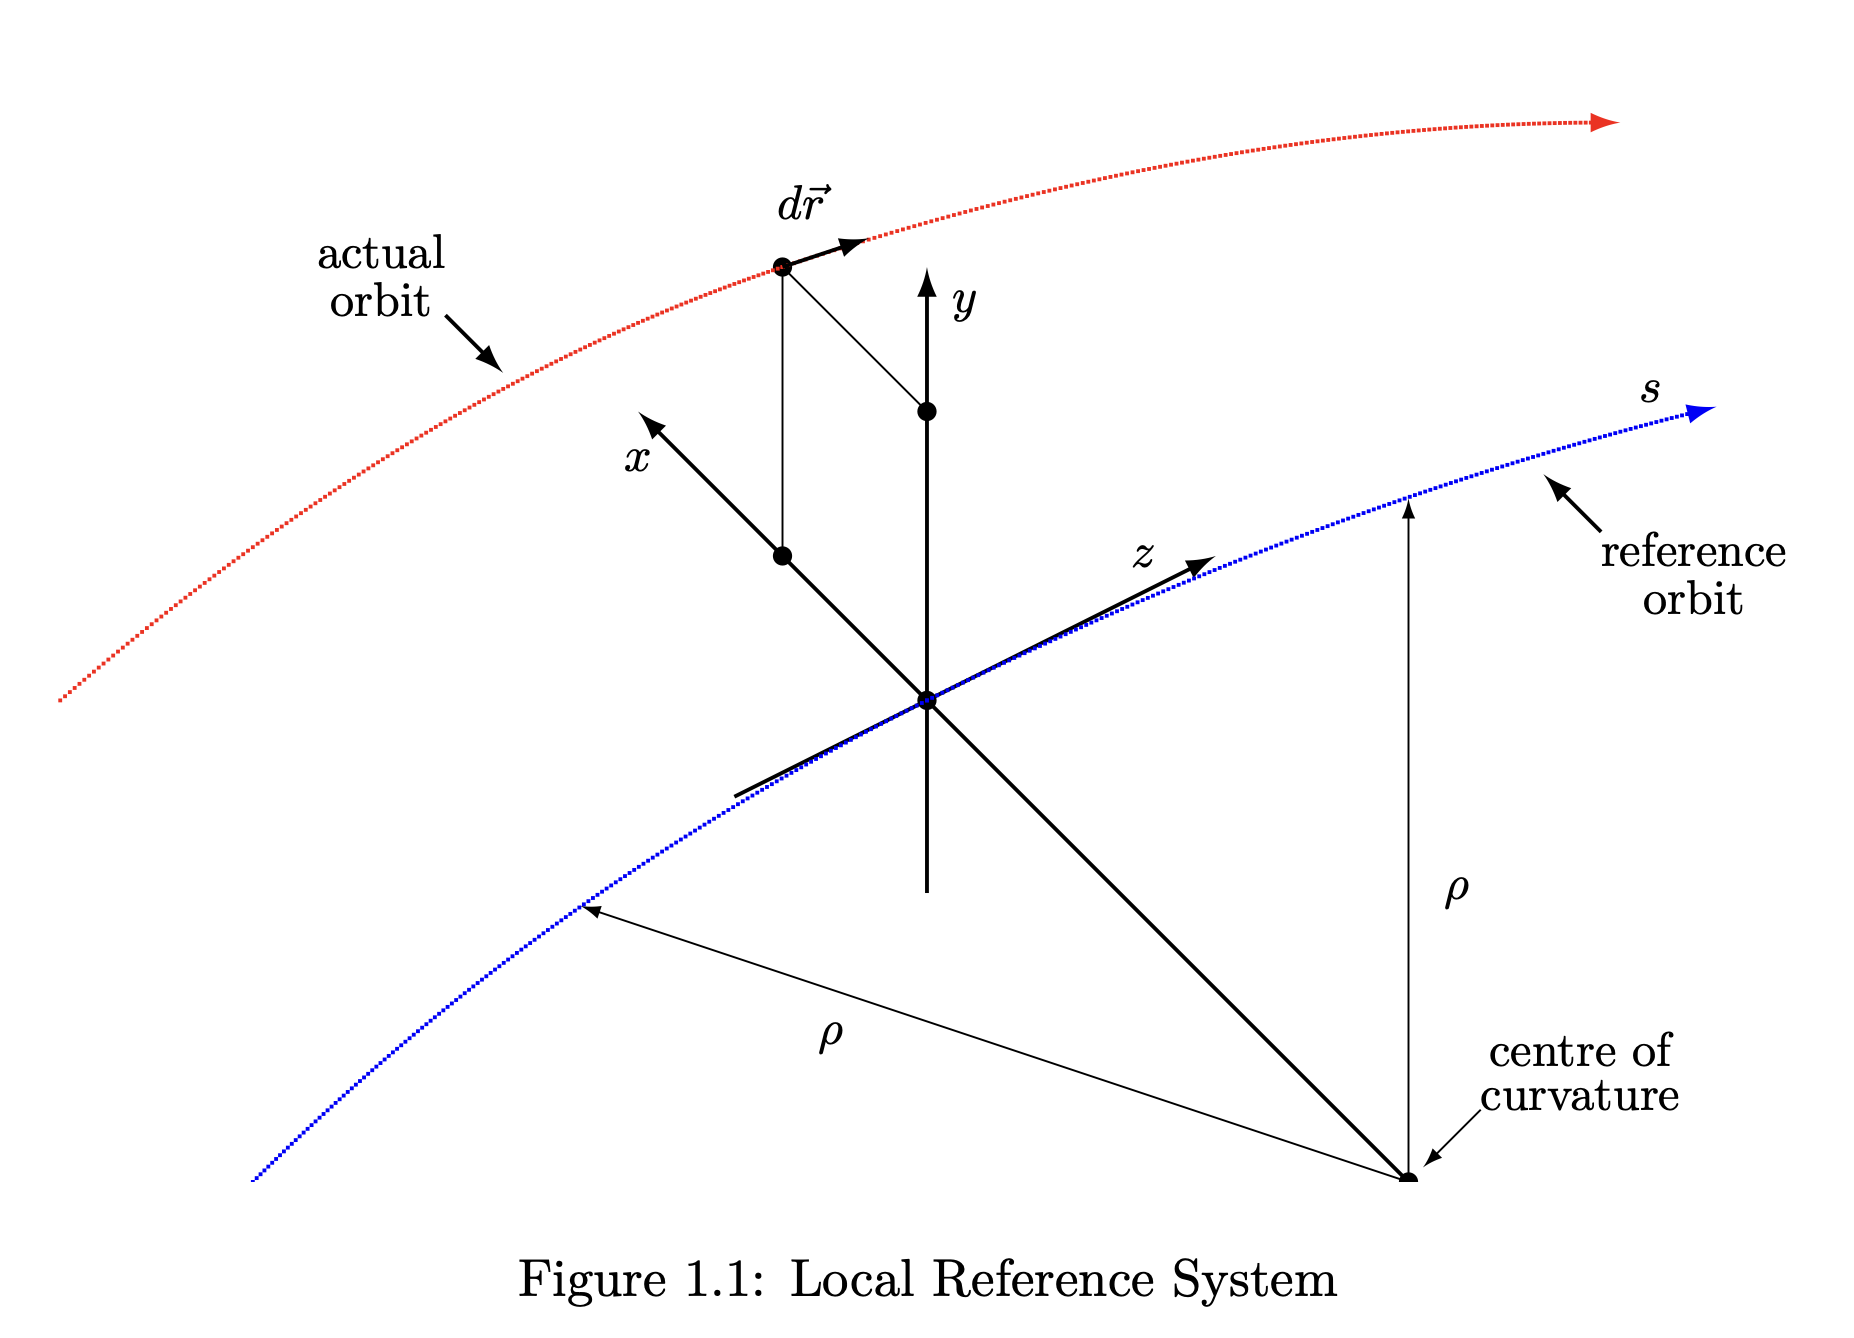
\includegraphics[width=0.80\textwidth, trim={0cm 2cm 0cm 1cm}, clip]{figures/local_frame.png}
  \caption{Local Reference System}
  \label{fig:local-frame}
\end{figure}

The beam line or ring to be studied is described as a sequence of beam elements
placed sequentially along a reference trajectory.

The reference trajectory consists of a series of straight line segments and circular arcs.
The accompanying tripod, as shown in Fig.~\ref{fig:local-frame}, spans a local curvilinear
right-handed coordinate system $(x,y,s)$. The local $s$-axis is the tangent to the reference
orbit and $x$ and $y$ are perpendicular to $s$. Typically, $x$ is horizontal and $y$ vertical.

We call $\rho$ the local radius of curvature of the reference trajectory and $h$
the local curvature defined as:
\begin{align}
  h = \frac{1}{\rho}
\end{align}

\section{Global reference system}

This section is adapted from \cite{madsite}.
~\\

The local reference system $( x, y, s )$ may thus be referred to a global Cartesian
coordinate system $( X, Y, Z )$ as shown in Fig.~\ref{fig:global-frame}.

\begin{figure}[h]
  \centering
  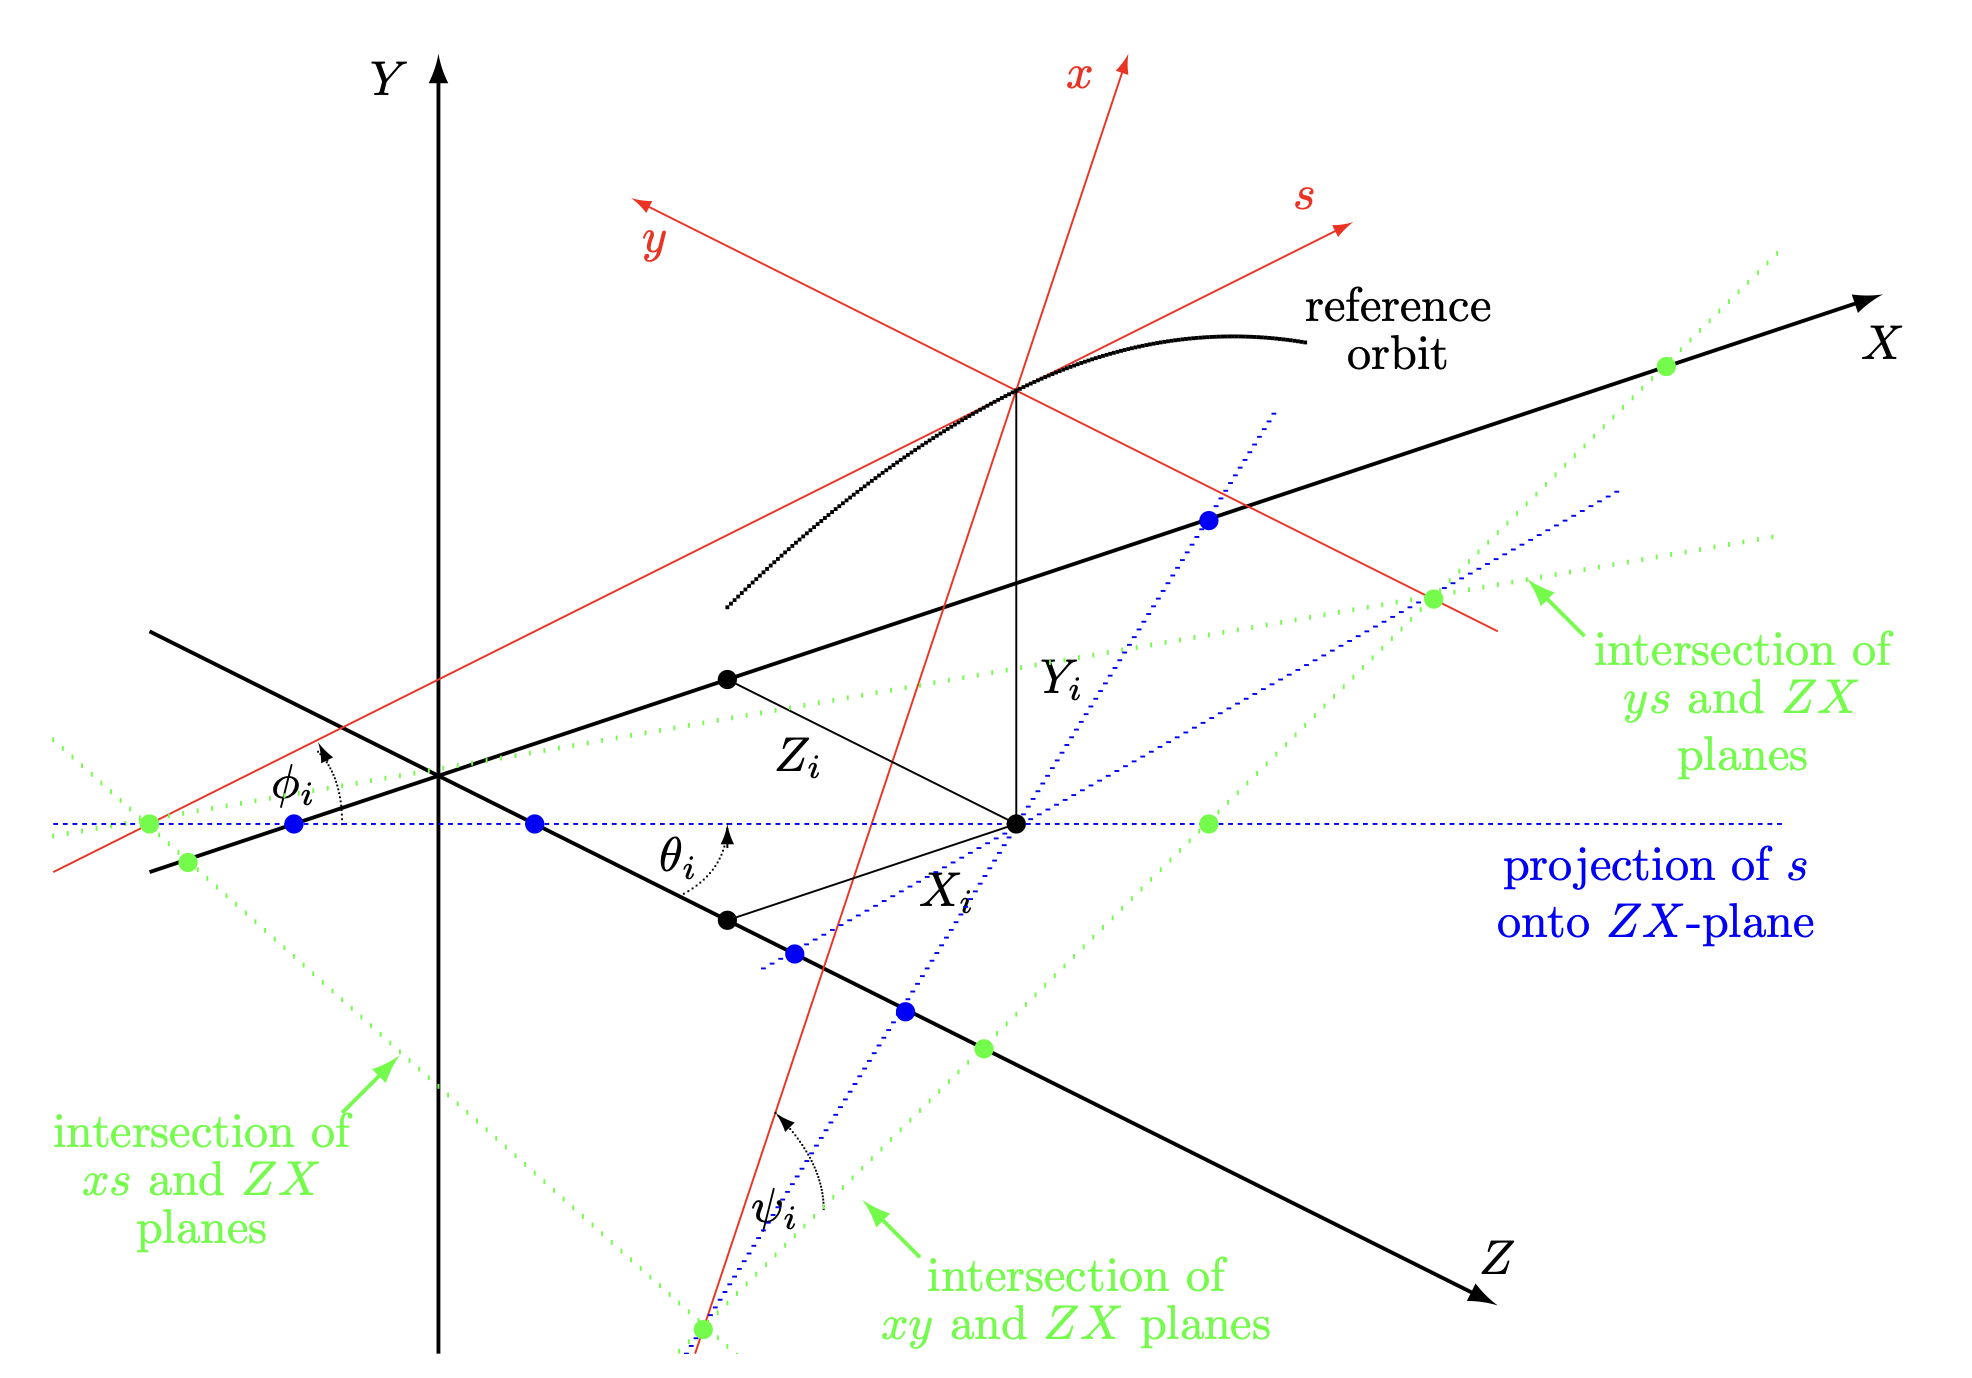
\includegraphics[width=0.9\textwidth]{figures/global_frame.png}
  \caption{Global Reference System showing the global Cartesian system $( X,Y,Z )$ in black
           and the local reference system $( x, y, s )$ in red with the translation $( X_i,Y_i,Z_i)$ and
           rotation $(\theta_i,\phi_i,\psi_i)$ relating the two.}
  \label{fig:global-frame}
\end{figure}

The positions between beam elements are indexed with $i=0,\ldots,n$. The local reference system
$(x_i,y_i,s_i)$ at position $i$, i.e. the displacement and direction of the reference orbit with respect
to the system $( X, Y, Z )$ are defined by three displacements $( X_i,Y_i,Z_i)$ and three angles
$( \theta_i,\phi_i,\psi_i)$.

The above quantities are defined more precisely as follows:

\begin{itemize}
  \item $X$ Displacement of the local origin in $X$-direction.
  \item $Y$ Displacement of the local origin in $Y$-direction.
  \item $Z$ Displacement of the local origin in $Z$-direction.
  \item $\theta$ is the angle of rotation (azimuth) about the global $Y$-axis, between the
        global $Z$-axis and the projection of the reference orbit onto the $( Z,X)$-plane.
        A positive angle $\theta$ forms a right-hand screw with the $Y$-axis.
  \item $\phi$ is the elevation angle, i.e. the angle between the reference orbit and its projection onto the $( Z,X)$-plane. A positive angle $\phi$ corresponds to increasing
        $Y$.

        If only horizontal bends are present, the reference orbit remains in the $( Z,
        X)$-plane and $\phi$ is always zero.
  \item $\psi$ is the roll angle about the local $s$-axis, i.e. the angle between the line defined
        by the intersection of the $( x, y)$-plane and $( Z, X)$-plane on one hand, and the
        local $x$-axis on the other hand. A positive angle $\psi$ forms a right-hand screw
        with the $s$-axis.
\end{itemize}

Note that the angles $( \theta, \phi, \psi)$ do not follow the usual definition of Euler angles.
The reference orbit starts at the origin and
points by default in the direction of the positive $Z$-axis.

Internally the displacement is described by a vector $\mathbf{V}$ and the orientation by a unitary matrix
$\mathbf{W}$. The column vectors of $\mathbf{W}$ are the unit vectors spanning the local coordinate axes in the
order $( x, y, s )$. $\mathbf{V}$ and $\mathbf{W}$ have the values:
\begin{align}
  \mathbf{V} &=
    \begin{bmatrix}
      X\\
      Y\\
      Z
    \end{bmatrix},
  &
  \mathbf{W} &= \Theta \Phi \Psi
\end{align}
where
\begin{align}
  \Theta &=
    \begin{bmatrix}
      \cos\theta & 0 & \sin\theta\\
      0 & 1 & 0\\
      -\sin\theta & 0 & \cos\theta
    \end{bmatrix}, &
  \Phi &=
    \begin{bmatrix}
      1 & 0 & 0\\
      0 & \cos\phi & \sin\phi\\
      0 & -\sin\phi & \cos\phi
    \end{bmatrix}, &
  \Psi &=
    \begin{bmatrix}
      \cos\psi & -\sin\psi & 0\\
      \sin\psi & \cos\psi & 0\\
      0 & 0 & 1
    \end{bmatrix}.
\end{align}

When advancing
through a beam element, Xsuite (like MAD) computes $V_i$ and $W_i$ by the recurrence relations
\begin{align}
  V_i &= W_{i-1} R_i+V_{i-1}, &
  W_i &= W_{i-1} S_i
\end{align}
The vector $R_i$ is the displacement and the matrix $S_i$ is the rotation of the local reference
system introduced by the element $i$ with respect to the entrance of the same element. The
values of $R_i$ and $S_i$ are listed below for different physical element types.

In straight elements the local reference system is simply translated by the length of the element
along the local $s$-axis.

The corresponding $R$ and $S$ are
\begin{align}
  R &=
    \begin{bmatrix}
      0\\
      0\\
      L
    \end{bmatrix},
  &
  S &=
    \begin{bmatrix}
      1 & 0 & 0\\
      0 & 1 & 0\\
      0 & 0 & 1
    \end{bmatrix}.
\end{align}
A rotation of the element about the $s$-axis has no effect on $R$ and $S$, since the rotations of
the reference system before and after the element cancel.

Bending magnets have a curved reference orbit. For both rectangular and sector bending
magnets, the $R$ and $S$ are expressed as functions of the bend angle $\alpha$:
\begin{align}
  R &=
    \begin{bmatrix}
      \rho(\cos \alpha-1)\\
      0\\
      \rho\sin\alpha
    \end{bmatrix},
  &
  S &=
    \begin{bmatrix}
      \cos\alpha & 0 & -\sin\alpha\\
      0 & 1 & 0\\
      \sin\alpha & 0 & \cos \alpha
    \end{bmatrix}
\end{align}
where we have assumed that the bending occurs in the horizontal plane.
A positive bend angle represents a bend to the right, i.e. towards negative $x$ values. For
sector bending magnets, the bend radius is given by $\rho$, and for rectangular bending magnets
it has the value $\rho=L/(2 \sin( \alpha/2))$. If the magnet is rotated about the $s$-axis by an
angle $\psi$, $R$ and $S$ are transformed by
\begin{align}
  R &= T R, &
  S &= T S T^{-1}
\end{align}
where $T$ is the orthogonal rotation matrix
\begin{align}
  T &=
    \begin{bmatrix}
      \cos \psi & -\sin \psi & 0\\
      \sin \psi & \cos \psi & 0\\
      0 & 0 & 1
    \end{bmatrix}
\end{align}
The special value $\psi=\pi/2$ represents a bend down.

\section{Reference particle}

We introduce a reference particle with rest mass $m_0$, charge $q_0$, total energy $E_0$,
momentum $P_0$, and relativistic factors $\beta_0,\gamma_0$. These quantities satisfy
\begin{align}
  E_0^2 &= (P_0 c)^2 + (m_0 c^2)^2, \\
  E_0 &=  m_0 \gamma_0 c^2, \\
  P_0 &= m_0 \beta_0 \gamma_0 c, \\
  \beta_0 &= \frac{P_0 c}{E_0} = \sqrt{1-\frac{1}{\gamma_0^2}}, \\
  \gamma_0 &= \frac{1}{\sqrt{1-\beta_0^2}} .
\end{align}
The reference particle will be used to normalize momentum and energy variables as
well as electromagnetic fields and potentials.
For this purpose we introduce the corresponding reference beam rigidity as
\begin{align}
  \label{eq:brigidity}
  \mathrm{rig}_0 = \frac{P_0}{q_0},
\end{align}
which is the momentum per unit charge used, for example, to normalize multipole strengths.

\section{Electromagnetic potentials and fields}
\label{sec:electromagnetic_potentials_and_fields}
The electromagnetic fields {\bf E} and {\bf B} can be derived from the potentials $\Phi(x,y,s,t)$ and $\mathbf{A}(x,y,s,t)$, where
\begin{align}
\mathbf{A}(x,y,s,t)=A_x(x,y,s,t) \hat x(s) + A_y(x,y,s,t) \hat y(s) + A_s(x,y,s,t) \hat z(s)
\end{align}
and for which:
\begin{align}
  \mathbf{E}  &= -\nabla \Phi - \frac{\partial \mathbf{A}}{\partial t}
               = -\partial_x \Phi \hat x - \partial_y \Phi \hat y -
  \frac{1}{1+h x}  \partial_s \Phi \hat z - \partial_t \mathbf{A}\\
  \mathbf{B} &= \nabla\times\mathbf{A}  =
  \left(\partial_y A_s - \frac{\partial_s  A_y}{1+h x} \right) \hat x
  +\left(\frac{\partial_s A_x-\partial_x (1+h x) A_s }{1+h x} \right)\hat y
  + \left(\partial_x A_y - \partial_y A_x \right) \hat z. \label{eq:Bfield_from_a_curved}
\end{align}

We use the reference particle properties to define normalized potentials:
\begin{align}
  &\mathbf{a}(x,y,s,t) = \frac{q_0}{P_0} \mathbf{A}(x,y,s,t)\\
  &\varphi(x,y,s,t) =
    \frac{q_0}{P_0c}\Phi(x,y,s,t)
\end{align}



\section{Convention for multipole expansion of magnetic fields}
\label{sec:multipole_expansion}

This section is adapted from \cite{madsite}.

\subsection{Straight magnets ($h=0$)}

Xsuite, like MAD, uses the following Taylor expansion for the magnetic field components.
Using a complex notation for the field $(B_y+i B_x)$ and the position $(x+i y)$ we write:

\begin{align}
  B_y+i B_x=\sum_{n=0}^{\infty} \frac{(B_n+i A_n)}{n !}(x+i y)^{n}
\end{align}
where, assuming that the field is piece-wise constant along $s$ and that the local
curvature $h$ is zero, the coefficients $B_n$ and $A_n$ are the on-axis
derivatives of the transverse field components:
\begin{align}
  B_n &= \left.\frac{\partial^n B_y}{\partial x^n}\right|_{x=0,\,y=0}, &
  A_n &= \left.\frac{\partial^n B_x}{\partial x^n}\right|_{x=0,\,y=0}.
\end{align}

The associated longitudinal vector potential for straight elements can be written as
\begin{align}
  A_s(x,y) = -\,\Re\left(\sum_{n=0}^{\infty} \frac{(B_n+i A_n)}{(n+1) !}(x+i y)^{n+1}\right),
\end{align}
so that $B_y+i B_x = -(\partial_x - i \partial_y) A_s$ yields the field expansion above.

We define the normal multipole coefficients $K_n$ and the skew multipole coefficients
$\hat{K}_n$ using the reference beam rigidity from Eq.~\eqref{eq:brigidity}:
\begin{align}
  K_n=\frac{B_n}{\mathrm{rig}_0}
\end{align}
and
\begin{align}
  \hat{K}_n=\frac{A_n}{\mathrm{rig}_0}
\end{align}

Using these coefficients, the field expansion and the longitudinal vector potential
can be written as
\begin{align}
  B_y+i B_x &= \mathrm{rig}_0
  \sum_{n=0}^{\infty} \frac{(K_n+i \hat{K}_n)}{n !}(x+i y)^{n}, \\
  A_s(x,y) &= -\,\mathrm{rig}_0\,\Re\left(\sum_{n=0}^{\infty}
  \frac{(K_n+i \hat{K}_n)}{(n+1) !}(x+i y)^{n+1}\right).
\end{align}
The normalized longitudinal potential $a_s$ introduced in
Sec.~\ref{sec:electromagnetic_potentials_and_fields} is then
\begin{align}
  a_s(x,y) &= \frac{q_0}{P_0} A_s(x,y)
  = -\,\Re\left(\sum_{n=0}^{\infty}
  \frac{(K_n+i \hat{K}_n)}{(n+1) !}(x+i y)^{n+1}\right).
\end{align}
In the special case where only $K_0$, $K_1$, and $K_2$ are non-zero (all $K_{n\ge3}=0$
and $\hat{K}_n=0$), the normalized longitudinal potential reduces to
\begin{align}
  a_s(x,y) &= -\left[
  K_0 x + \frac{K_1}{2}\left(x^2 - y^2\right)
  + \frac{K_2}{6}\left(x^3 - 3 x y^2\right) \right].
\end{align}

\subsection{Curved magnets ($h\neq0$)}

In the case of curved magnets ($h\neq0$), multipole components are still defined
as the derivatives at the symmetry point of the magnet:
\begin{align}
  B_n &= \left.\frac{\partial^n B_y}{\partial x^n}\right|_{x=0,\,y=0}, \label{eq:multipole_Bn} \\
  A_n &= \left.\frac{\partial^n B_x}{\partial x^n}\right|_{x=0,\,y=0} . \label{eq:multipole_An}
\end{align}
and the corresponding normalized multipole coefficients $K_n$ and $\hat{K}_n$ are defined as before:
\begin{align}
  K_n=\frac{B_n}{\mathrm{rig}_0}, \quad &
  \hat{K}_n=\frac{A_n}{\mathrm{rig}_0}.
\end{align}
The field and potential expansions are more complex than in the straight case
as they must satisfy Eq.~\ref{eq:Bfield_from_a_curved} together with the definitions \eqref{eq:multipole_Bn}
and \eqref{eq:multipole_An}.

For the special case where only $K_0$, $K_1$, and $K_2$ are non-zero, a truncated expansion
for the normalized potential is:
\begin{align}
a_s(x,y,s)
&= -K_0\left(x-\frac{h x^{2}}{2(1+h x)}\right)
 -K_1\left(\frac{1}{2}(x^{2}-y^{2})-\frac{h}{6}x^{3}\right) \nonumber\\
&\quad -K_2\left(\frac{1}{6}(x^{3}-3xy^{2})-\frac{h}{24}(x^{4}-y^{4})\right)
\label{eq:as_curved}
\end{align}


\section{Particle coordinates}

Xsuite uses as independent variable the position along the reference trajectory $s$.
We call $t$ the time coordinate, i.e. the time at which the particle passes
the position $s$.

Xsuite can track particles of different species within the same particle ensemble.
We call $m$ and $q$ the rest mass and charge of the individual particle and we introduce
the coefficient:
\begin{align}
  \chi = \frac{q}{q_0} \frac{m_0}{m}
\end{align}

In the ``longitudinal plane'', i.e. the space spanned by time and energy coordinates,
we can use any of the following pairs of conjugate variables:
\begin{align}
\xi &= s \frac{\beta}{\beta_0} - \beta c t &
\tau &= \frac{s}{\beta_0} - ct &
\zeta &= s - \beta_0 ct \label{eq:coord1}&
\delta &=
  \frac{P \frac{m_0}{m} -P_0}{P_0} \\
\delta &=
  \frac{P \frac{m_0}{m} -P_0}{P_0} &
p_\tau &=
  \frac{1}{\beta_0} \frac{E \frac{m_0}{m} -E_0}{E_0} &
p_\zeta &=
  \frac{1}{\beta_0^2}\frac{E \frac{m_0}{m} -E_0}{E_0}&
\ell &= \beta c t
  \label{eq:coord2}
\end{align}
where variables in the same column are canonically conjugate.

These variables can be easily related to each other:
\begin{align}
  &E =  m \gamma c^2 = P_0 c \left( p_\tau + \frac{1}{\beta_0}\right), \\
  &P = m \beta \gamma c = P_0 (1 + \delta) \\
  &\beta = \frac{P c}{E} = \sqrt{1-\frac{1}{\gamma^2}} =\sqrt{1 - \frac{1 - \beta_0}{\left(1 + \beta_0 p_\tau\right)^2}}, \\
  &\gamma = \frac{1}{\sqrt{1-\beta^2}} = \gamma_0 (1 + \beta_0 p_\tau)\\
  &\xi= s \frac{\beta}{\beta_0} - \ell =
      \beta\tau =
      \frac{\beta}{\beta_0}\zeta \\
  &\delta= \sqrt{p_\tau^2 + 2 \frac{p_\tau}{\beta_0} +1} - 1
       =\beta p_\tau + \frac{\beta-\beta_0}{\beta_0}\\
  &\delta= \sqrt{\beta_0^2p_\zeta^2 + 2 p_\zeta +1} - 1
      =\beta\beta_0 p_\zeta + \frac{\beta-\beta_0}{\beta_0}\\
  &(1+\delta)^2 = \frac{P^2}{P_0^2} = \frac{E^2 - m_0^2 c^4}{P_0^2 c^2}
     = \frac{E^2}{c^2 P_0^2} - \frac{1}{\beta_0^2 \gamma_0^2}
     = \left( p_\tau + \frac{1}{\beta_0}\right)^2 - \frac{1}{\beta_0^2 \gamma_0^2}
     \label{eq:one_plus_delta_squared}\\
  &p_\tau = \beta_0 p_\zeta\\
  &p_\tau = \frac{\sqrt{1 + \beta_0^2\,\delta(\delta + 2)} - 1}{\beta_0}
\end{align}
and the following derivatives:
\begin{align}
    &\frac{\partial \delta}{\partial p_\tau} =
    \frac{p_\tau+1/\beta_0}{1+\delta} = \frac{1}{\beta} \\
  &\frac{\partial}{\partial\delta}\left(
    \frac{1+\delta}{\beta\beta_0}
  \right)=
    \frac{\beta}{\beta_0}
\end{align}

For small energy deviations ($\delta \ll 1$, $p_\tau \ll 1$, $p_\zeta \ll 1$),
we can neglect the terms of order $\delta^2$, $p_\tau^2$, $p_\zeta^2$ and higher, hence
the following approximations hold:
\begin{align}
  &\delta \simeq \frac{p_\tau}{\beta_0} \\
  &\delta \simeq p_\zeta \label{eq:delta_pzeta_approx}\\
  &\beta \simeq \beta_0 + (1 - \beta_0^2) p_\tau
\end{align}

In the transverse plane we use the coordinates $x, p_x, y, p_y$. The transverse canonical
momenta are defined as:
\begin{align}
  p_x&= \frac{m_0}{m}\frac{P_x}{P_0}, &
  p_y&= \frac{m_0}{m}\frac{P_y}{P_0},
\end{align}
where:
\begin{align}
  P_x &= m \gamma \dot x + q A_x, &
  P_y &= m \gamma \dot y + q A_y
\end{align}
in which $\dot x$ and $\dot y$ are the time derivatives of $x$ and $y$.

\section{Hamiltonian and equations of motion}

The motion of a particle is described by one of the following Hamiltonian functions,
depending on the choice of longitudinal coordinates:
\begin{align}
 H_\delta   &= \frac{1+\delta}{\beta\beta_0} - (1+h x) \left(
      \sqrt{ \left(\frac{1+\delta}{\beta}-\chi\varphi\right)^2
           - \frac{1}{\beta_0^2\gamma_0^2}
           - (p_x - \chi a_x)^2
           - (p_y - \chi a_y)^2}
       + \chi a_s
    \right) \\
 H_\tau   &= \frac{p_\tau}{\beta_0} - (1+h x) \left(
      \sqrt{ \left(p_\tau+\frac{1}{\beta_0}-\chi\varphi\right)^2
           - \frac{1}{\beta_0^2\gamma_0^2}
           - (p_x - \chi a_x)^2
           - (p_y - \chi a_y)^2}
       + \chi a_s
    \right) \label{eq:hamiltonian_htau}\\
  H_\zeta &= p_\zeta - (1+h x) \left(
      \sqrt{ \left(\beta_0 p_\zeta+\frac{1}{\beta_0}-\chi\varphi\right)^2
           - \frac{1}{\beta_0^2\gamma_0^2}
           - (p_x - \chi a_x)^2
           - (p_y - \chi a_y)^2}
       + \chi a_s
    \right)
\end{align}

Using $\tau$ and $p_\tau$ as longitudinal coordinates, the equations of motion are:
\begin{align}
  \frac{\text{d} p_x}{\text{d}s} &=
    -\frac{\partial H_\tau}{\partial x} \\
  \frac{\text{d} p_y}{\text{d}s} &=
    -\frac{\partial H_\tau}{\partial y} \\
  \frac{\text{d} p_\tau}{\text{d}s} &=
    -\frac{\partial H_\tau}{\partial \tau} \\
  \frac{\text{d} x}{\text{d}s} &=
    \frac{\partial H_\tau}{\partial p_x} \\
  \frac{\text{d} y}{\text{d}s} &=
    \frac{\partial H_\tau}{\partial p_y} \\
  \frac{\text{d} \tau}{\text{d}s} &=
    \frac{\partial H_\tau}{\partial p_\tau}
\end{align}

The full derivation of the Hamiltonian and equations of motion can be found in
Wolski~\cite{wolski2014beam} (note the different notation, as the symbol $\delta$
in~\cite{wolski2014beam} denotes the quantity that here we call $p_\tau$).

\section{Expanded magnet body Hamiltonian}

For a magnet with piece-wise constant multipole components and curvature $h$, we can
set $a_x = 0$ and $a_y = 0$ in Eq.~\eqref{eq:hamiltonian_htau}:
\begin{align}
 H_\tau   &= H^\text{kin} + H^\text{magn}
\end{align}
where
\begin{align}
  &H^\text{kin} = \frac{p_\tau}{\beta_0} - (1+h x) \sqrt{ \left(p_\tau+\frac{1}{\beta_0}\right)^2
           - \frac{1}{\beta_0^2\gamma_0^2}
           - p_x^2
           - p_y^2} \label{eq:hamilt_kinetic_part}\\
  &H^\text{magn} = -(1+h x) \chi a_s
\end{align}

\subsection{Approximation of the kinetic part of the Hamiltonian}

Using Eq.~\ref{eq:one_plus_delta_squared}, the kinetic part can be rewritten as follows:
\begin{align}
  H^\text{kin}
    &= \frac{p_\tau}{\beta_0} - (1+h x) \sqrt{ (1 + \delta)^2  - p_x^2 - p_y^2}\\
    &= \frac{p_\tau}{\beta_0} - \sqrt{ (1 + \delta)^2 - p_x^2 - p_y^2}
                              - h x \sqrt{ (1 + \delta)^2  - p_x^2 - p_y^2}
\end{align}
Neglecting high-order terms $h^2 x^2 p_x^2$ and $h^2 x^2 p_y^2$ in the second
square root, we can approximate:
\begin{align}
  H^\text{kin}
    &= \frac{p_\tau}{\beta_0} - \sqrt{ (1 + \delta)^2 - p_x^2 - p_y^2} - h x (1 + \delta)\\
    &= H_D - h x (1 + \delta)
    \label{eq:hamilt_kinetic_curv_approx}
\end{align}
where
\begin{align}
  H_D = \frac{p_\tau}{\beta_0} - \sqrt{ (1 + \delta)^2 - p_x^2 - p_y^2}
\end{align}
is the Hamiltonian of a straight drift.

The Hamiltonian for the drift can in turn be expanded as follows:
\begin{align}
  H_D &= \frac{p_\tau}{\beta_0} - (1 + \delta)\sqrt{1  - \frac{p_x^2 + p_y^2}{(1 + \delta)^2}}\\
      &\simeq \frac{p_\tau}{\beta_0} - (1 + \delta) + \frac{1}{2}\frac{p_x^2 + p_y^2}{(1 + \delta)}
      \label{eq:hamilt_drift_expanded}
\end{align}

Replacing Eq.~\eqref{eq:hamilt_drift_expanded} in Eq.~\eqref{eq:hamilt_kinetic_curv_approx}
yields the following expression for the kinetic part of the Hamiltonian:
\begin{align}
  H^\text{kin}
    &\simeq  \frac{p_\tau}{\beta_0}
    - \left(1 + \delta  - \frac{1}{2}\frac{p_x^2 + p_y^2}{(1 + \delta)}\right)
    - h x \left(1 + \delta\right)
\end{align}

\subsection{Approximation of the magnetic part of the Hamiltonian}

For the common case where only $K_0$, $K_1$, and $K_2$ are non-zero, inserting
the curved-magnet potential from Eq.~\eqref{eq:as_curved} in $H^\text{magn}$ yields:
\begin{align}
  H^\text{magn} &= (1+h x)\chi \Bigg[
    K_0\left(x-\frac{h x^{2}}{2(1+h x)}\right)
    + K_1\left(\frac{1}{2}(x^{2}-y^{2})-\frac{h}{6}x^{3}\right) \nonumber\\
  &\qquad\quad
    + K_2\left(\frac{1}{6}(x^{3}-3xy^{2})-\frac{h}{24}(x^{4}-y^{4})\right)
  \Bigg].
\end{align}
Discarding all terms nonlinear in $h$ (i.e., keeping only $\mathcal{O}(h)$) yields
\begin{align}
  H^\text{magn} &\simeq \chi \Bigg[
    K_0 x
    + K_1 \frac{x^{2}-y^{2}}{2}
    + K_2 \frac{x^{3}-3xy^{2}}{6}
  \Bigg] \nonumber\\
  &\quad + \chi h \Bigg[
    \frac{K_0}{2} x^{2}
    + K_1 \left(\frac{1}{3}x^{3}-\frac{1}{2}x y^{2}\right)
    + K_2 \left(\frac{1}{8}x^{4}-\frac{1}{2}x^{2}y^{2}+\frac{1}{24}y^{4}\right)
  \Bigg].
\end{align}


\section{Symplectic integrators and magnet models}\label{sec:symplectic_integrators}

In Xsuite, magnets are modeled using symplectic integrators, splitting the Hamiltonian
into a `propagation' part and a `kick' part, for which closed-form solutions of the equations of motion
are available.

Hamiltonians for which closed-form solutions of the equations of motion exist and are
implemented in Xsuite are reported in Table~\ref{tab:maps}. The corresponding
maps are reported in Chapter~\ref{chapter:beam_element_maps}.

Different magnet models are available, which correspond to different ways of splitting
the Hamiltonian. The available models are reported in Table~\ref{tab:models} and
the available integration schemes are reported in Table~\ref{tab:integrators}.

\begin{table}[htb]
\centering
{\small
\begin{tabular}{llll}
\toprule
\textbf{Map} & \textbf{Params.} & \textbf{Description} \\
\midrule
D   &            & Drift exact   &
$H_D = \frac{p_\tau}{\beta_0} - \sqrt{(1 + \delta)^2 - p_x^2 - p_y^2}$ \\
De  &            & Drift expanded &
$H_{De} = \frac{p_\tau}{\beta_0} - (1 + \delta) + \frac{1}{2}\frac{p_x^2 + p_y^2}{(1 + \delta)}$\\
Dc  &            & Exact drift correction &
$H_{Dc} = H_D - H_{De}$\\
R   & h         & Curved drift&
$H_R = \frac{p_\tau}{\beta_0} - (1+h x) \sqrt{(1 + \delta)^2 - p_x^2 - p_y^2}$\\
Br  & $K_0$        & Rectangular bend &
$H_{Br} = H_D + \chi K_0 x$
\\
B   & $K_0$, h     & Exact Bend &
$H_{B} = H_R + \chi K_0 x + \chi h K_0 \frac{x^2}{2}$\\
K0  & $K_0$           & Dipole kick &
$H_{K0} = \chi K_0 x$\\
K1  & $K_1$       & Quadrupole kick &
$H_{K1} = \chi K_1\frac{x^2 - y^2}{2}$\\
h  & $h$         & Curvature kick &
$H_{h} = -h x (1 + \delta)$\\
K0h & $K_0$          & Weak focusing kick &
$H_{K0h} = \chi h K_0  \frac{x^2}{2}$\\
K1h & $K_1$, $h$      & Quad curv. correction &
$H_{K1h} = \chi h K_1 \frac{2 x^3 - 3 xy^2}{6}$\\
Kn  & $K_n$, $\hat{K}_n$     & Multipole &
$H_{Kn} = \chi \Re\left( \sum_{n=0}^N (K_n+i{\hat K}_n)\frac{(x+iy)^{n+1}}{(n+1)!}\right)$
\\
% Knh & kn, ks, h  & Curved Multipoles &
% Not yet available\\
M   & $K_0$, $K_1$, $h$ & Expanded bend-quad. &
$H_{M} =  H_{De} - h x (1 + \delta) + \chi K_0 x + \chi K_1\frac{x^2 - y^2}{2} + \chi h K_0 \frac{x^2}{2}$\\
S   & $K_s$          & Solenoid &
$H_{S} = \frac{p_\tau}{\beta_0} - \sqrt{(1 + \delta)^2 - \left(p_x-\frac{K_s}{2} y\right)^2 - \left(p_y+\frac{K_s}{2}\right)^2}$
\\
\bottomrule
\end{tabular}
}
\caption{Hamiltonians of the implemented maps.
        \label{tab:maps}}
\end{table}


\begin{table}[t]
\centering
\begin{tabular}{lll}
\toprule
\textbf{Model} & \textbf{Propagation part} & \textbf{Kick part} \\
\midrule
rot-kick-rot-low-order & [R] & [K0 K0h K1 K1h Kn] \\
rot-kick-rot & [R, K0] - Yoshida 4 & [K0h K1 K1h Kn] \\
rot-kick-rot-high-order & [R, K0] - Yoshida 6 & [K0h K1 K1h Kn] \\
bend-kick-bend & [B] & [K1 K1h Kn] \\
mat-kick-mat & [M] & [K1h Kn] \\
mat-kick-mat-exact ($h=0$) & [M] & [Dc/2, Kn, Dc/2] \\
drift-kick-drift-exact & [D] & [h K0 K0h K1 K1h Kn] \\
drift-kick-drift-expanded & [De] & [h K0 K0h K1 K1h Kn] \\
\bottomrule
\end{tabular}
\caption{Available magnet models. For \texttt{mat-kick-mat-exact}, the kick
is bracketed by two half-length correction maps; see
Sec.~\ref{sec:mat_kick_mat_exact}. \label{tab:models}}
\end{table}


\begin{table}[t]
\centering
\begin{tabular}{lcccp{6.5cm}}
\toprule
\textbf{Integrator} & \textbf{$n_\text{kicks}$} & \textbf{$n_\text{drifts}$} & \textbf{Order} & \textbf{Description}\\
\midrule
uniform & 1 & 2 & 2nd &
    Kicks uniformly distributed along the length of the element
    (leapfrog, eq.~(2.10) of \cite{yoshida90}) \\
teapot & 1 & 2 & 2nd &
    TEAPOT integration scheme \cite{Talman:533900, Burkhardt:2013eua} \\
yoshida-4 & 3 & 4 & 4th &
    Fourth-order Yoshida integrator, eq.~(2.11) of \cite{yoshida90} \\
yoshida-6 & 7 & 8 & 6th &
    Sixth-order Yoshida integrator, table 1, variant A, of \cite{yoshida90}.
    Default (``adaptive'') integrator \\
yoshida-8 & 15 & 16 & 8th &
    Eighth-order Yoshida integrator, table 2, variant D, of \cite{yoshida90},
    as also used by MAD-NG \cite{madng_github} \\
\bottomrule
\end{tabular}
\caption{Available integration schemes. \label{tab:integrators}}
\end{table}

\subsection{Practical recommendations}

\begin{itemize}
\item The \texttt{bend-kick-bend} model is an exact map for a pure dipole ($K_0$)
    with curvature $h$, so if there is no \texttt{K1} or higher multipole component,
    the map is exact for any \texttt{nslice}, so \texttt{nslice=1} suffices and
    increasing the order or slicing will only increase the computational cost and
    numerical error.
\item Otherwise (e.g.\ $K_1$, $K_2$, \dots, or skew components present),
    prefer a higher-order integrator (\texttt{yoshida-6} is typically best)
    with as few slices as possible over a low-order one
    (\texttt{uniform}, \texttt{teapot}) with many slices: increasing the
    order is roughly equivalent, in terms of accuracy, to increasing
    \texttt{nslice} by a factor 10 while keeping a lower order (e.g.\
    fourth order with \texttt{nslice=10} $\approx$ second order with
    \texttt{nslice=100}), but at a much lower computational cost.
\item Fewer, higher-order slices are more numerically stable as each
    drift step has some numerical error, so more slices means more
    accumulated error, not less.
\end{itemize}

\FloatBarrier



\chapter{Beam element maps}
\label{chapter:beam_element_maps}

This chapter presents the maps used to transport particles through beam
elements. Depending on the element and the chosen model, these maps are
used individually or combined by the symplectic integrators described in
Section~\ref{sec:symplectic_integrators}. In the latter case, propagation
and kick maps are composed to approximate the evolution under the full
Hamiltonian.

\section{Drift}

Implemented in the \href{https://xsuite.readthedocs.io/en/latest/apireference.html#drift}{\underline{Drift element}}.
~\\

A drift is a straight, field-free region ($h(x,y)=0$, $V=0$ and
$\mathbf{A}=0$).  The exact and expanded Hamiltonians for a drift space are
\begin{align}
  H_\tau =
    \frac{p_\tau}{\beta_0}  - \sqrt{(1+\delta)^2 - p_x^2 - p_y^2}
  &\approx
    \frac{p_\tau}{\beta_0} - \delta + \frac{1}{2}\frac{p_x^2+p_y^2}{1+\delta}.
\end{align}
% \begin{align}
%   H_\sigma = p_\sigma - \sqrt{(1+\delta)^2 - p_x^2 - p_y^2} &\approx
%   p_\sigma - \delta + \frac{1}{2}\frac{p_x^2+p_y^2}{1+\delta}.
% \end{align}

The corresponding maps can be obtained by solving the equations of motion:
\begin{align}
  \frac{\text{d} p_i}{\text{d}s} &= -\frac{\partial H}{\partial q_i} &
  \frac{\text{d} q_i}{\text{d}s} &=  \frac{\partial H}{\partial p_i}
\end{align}
As there is no explicit dependency on the position coordinates in the Hamiltonian, the
momenta remain unchanged in a drift.

For the position coordinates, we get:
\begin{align}
  \left(x\right)' &=
        \frac{p_x}{p_z}
        \approx \frac{p_x}{1+\delta} \\
  \left(y\right)' &=
        \frac{p_y}{p_z}
        \approx \frac{p_y}{1+\delta} \\
  \left(\tau\right)' &=
        \frac{1}{\beta_0} - \frac{1}{\beta}\frac{1+\delta}{p_z}
        \approx \frac{1}{\beta_0} - \frac{1}{\beta} - \frac{1}{\beta}
                \frac{p_x^2 + p_y^2}{2} \\
  p_z &=
        \sqrt{(1+\delta)^2 - p_x^2 - p_y^2}
\end{align}

Hence, the map relative to the expanded Hamiltonian for a drift of length $L$ is:
\begin{align}
  &x_p = \frac{p_x}{1+\delta} \\
  &y_p = \frac{p_y}{1+\delta}  \\
  &x  \leftarrow x + x_p L \\
  &y  \leftarrow y + y_p L \\
  &\zeta
    \leftarrow \zeta+
    l\left(1- \frac{\beta_0}{\beta}\left(1 + \frac{x_p^2+y_p^2}{2}\right)\right)
\end{align}
and the map relative to the exact Hamiltonian for a drift of length $L$ is:
\begin{align}
  &x \leftarrow x + \frac{p_x}{p_z} L\\
  &y \leftarrow y + \frac{p_y}{p_z} L\\
  &\zeta \leftarrow \zeta + L\left(
          1-\frac{\beta_0}{\beta}\frac{1+\delta}{p_z}
          \right)
\end{align}

\section{Polar drift (sector curvature $h$)}

Used in the implementation of \href{https://xsuite.readthedocs.io/en/latest/apireference.html#bend}{\underline{Bend}}
and \href{https://xsuite.readthedocs.io/en/latest/apireference.html#rbend}{\underline{RBend}} elements
when the model is ``rot-kick-rot''.
~\\
This map is ported from PTC and MAD-NG source codes.
~\\

The following map, corresponding to the motion of a particle in a field-free region
in a reference frame with horizontal curvature $h$,  is generated by the Hamiltonian:
\begin{equation}
H_R = \frac{p_\tau}{\beta_0} -(1 + hx) \left( \sqrt{(1 + \delta)^2 - p_x^2 - p_y^2}\right)
\end{equation}

We call:
\[
\delta_+ \equiv 1+\delta,\qquad \mathrm{rvv}=v/c,
\qquad s \equiv L.
\]

Define the longitudinal momentum component
\begin{equation}
p_z \equiv \sqrt{\delta_+^{\,2}-p_x^{\,2}-p_y^{\,2}} .
\end{equation}

Define the curvature radius
\begin{equation}
\rho \equiv \frac{1}{h},
\end{equation}
and the trigonometric abbreviations
\begin{equation}
c \equiv \cos(hs),\qquad
s_a \equiv \sin(hs),\qquad
s_{a2}\equiv \sin\!\left(\frac{hs}{2}\right).
\end{equation}

Introduce
\begin{equation}
\frac{1}{p_z} \equiv p_z^{-1},\qquad
p_{x,t} \equiv \frac{p_x}{p_z},
\qquad
\mathcal{D} \equiv c - s_a\, p_{x,t},
\qquad
\mathcal{D}^{-1} \equiv \frac{1}{\mathcal{D}}.
\end{equation}

Define also
\begin{equation}
p_s \equiv (x+\rho)\, s_a\, p_z^{-1}\, \mathcal{D}^{-1}.
\end{equation}

\paragraph{Transverse map}
\begin{align}
x_1 &=
\left[
x+\rho\left(2 s_{a2}^{\,2}+ s_a\, p_{x,t}\right)
\right]\mathcal{D}^{-1},
\\
p_{x1} &= c\,p_x + s_a\, p_z,
\\
y_1 &= y + p_s\, p_y.
\end{align}

\paragraph{Path length / longitudinal map}

The quantity \(\Delta \ell\) computed in the code is
\begin{equation}
\Delta \ell
=
\delta_+\,
\frac{(x+\rho)\, s_a}{c\, p_z\left(1-\dfrac{p_x s_a}{c\,p_z}\right)} .
\end{equation}

The longitudinal coordinate is updated as
\begin{equation}
\zeta_1 = \zeta + \left( L - \frac{\Delta \ell}{\mathrm{rvv}} \right),
\end{equation}
and the reference longitudinal position as
\begin{equation}
s_{\text{ref},1} = s_{\text{ref}} + L.
\end{equation}


\section{Curved exact bend}

Implemented in the \href{https://xsuite.readthedocs.io/en/latest/apireference.html#bend}{\underline{Bend element}}.
~\\

The generating Hamiltonian is:
\begin{equation}
H_{B} = \frac{p_\tau}{\beta_0} -(1 + hx) \left( \sqrt{(1 + \delta)^2 - p_x^2 - p_y^2} -K_0\left(x-\frac{hx^2}{2(1+hx)} \right) \right)
\end{equation}

For compactness, define
\begin{align}
p_w &= \sqrt{(1+\delta)^2-p_y^2}, \\
p_z(0) &= \sqrt{(1+\delta)^2-p_x(0)^2-p_y^2}, \\
p_z(s) &= \sqrt{(1+\delta)^2-p_x(s)^2-p_y^2}, \\
\Delta a(s) &=
\sin^{-1}\left(\frac{p_x(0)}{p_w}\right)
-\sin^{-1}\left(\frac{p_x(s)}{p_w}\right).
\end{align}

The corresponding map is adapted from \cite{forest99}:
\begin{align}
x(s) &= \frac{1}{hK_0 \chi} \left( h p_z(s) - \frac{dp_x(s)}{ds} - K_0 \chi \right) \\
p_x(s) &= p_x(0) \cos(h s) + \left( p_z(0) - K_0 \chi \left( \frac{1}{h} + x(0) \right) \right) \sin(h s) \\
y(s) &= y + \frac{p_y}{K_0\chi}\left[hs+\Delta a(s)\right] \\
p_y(s) &= p_y \\
\delta(s) &= \delta \\
\ell(s) &= \ell +
  \frac{1+\delta}{K_0\chi}\left[hs+\Delta a(s)\right]
\end{align}

\paragraph{Numerically stable horizontal update}

The direct evaluation of the horizontal coordinate can involve the subtraction
of large radius-like terms. In the implementation we compute the horizontal
increment
\begin{equation}
\Delta x(s) \equiv x(s)-x(0),
\end{equation}
and then update the coordinate as \(x(s)=x(0)+\Delta x(s)\). To derive a
stable expression for \(\Delta x(s)\), define
\begin{equation}
C = p_z(0)-K_0\chi\left(\frac{1}{h}+x(0)\right).
\end{equation}
Then
\begin{equation}
p_x(s)=p_x(0)\cos(hs)+C\sin(hs),
\end{equation}
and
\begin{equation}
\frac{1}{h}\frac{dp_x(s)}{ds}
=
C\cos(hs)-p_x(0)\sin(hs).
\end{equation}
The horizontal map can therefore be written as
\begin{equation}
x(s)=
\frac{p_z(s)-\left[C\cos(hs)-p_x(0)\sin(hs)\right]}{K_0\chi}
-\frac{1}{h}.
\end{equation}
Using the definition of \(C\), the initial coordinate satisfies
\begin{equation}
x(0)=
\frac{p_z(0)-C}{K_0\chi}
-\frac{1}{h}.
\end{equation}
Subtracting these two expressions gives the increment directly and avoids
reconstructing \(x(s)\) as a difference of large radius-like terms:
\begin{align}
\Delta p_z(s) &\equiv p_z(s)-p_z(0), \\
\Delta D(s) &\equiv C\cos(hs)-p_x(0)\sin(hs)-C.
\end{align}
Then
\begin{equation}
\Delta x(s)
=
\frac{\Delta p_z(s)-\Delta D(s)}{K_0\chi}.
\end{equation}
The second term is evaluated as
\begin{equation}
\Delta D(s)
=
C\left[\cos(hs)-1\right]-p_x(0)\sin(hs).
\end{equation}
For small \(hs\), the difference \(\cos(hs)-1\) is numerically inaccurate if
evaluated directly. We therefore use
\begin{equation}
\cos(hs)-1
=
-2\sin^2\left(\frac{hs}{2}\right),
\end{equation}
giving
\begin{equation}
\Delta D(s)
=
-2C\sin^2\left(\frac{hs}{2}\right)-p_x(0)\sin(hs).
\end{equation}
The first term is also evaluated without subtracting two nearly equal square
roots:
\begin{align}
\Delta p_z(s)
&=
\frac{p_z(s)^2-p_z(0)^2}{p_z(s)+p_z(0)} \\
&=
\frac{p_x(0)^2-p_x(s)^2}{p_z(s)+p_z(0)} \\
&=
\frac{\left[p_x(0)-p_x(s)\right]\left[p_x(0)+p_x(s)\right]}
{p_z(s)+p_z(0)}.
\end{align}
The implemented increment uses the expression above, with
\(\Delta p_z(s)\) and \(\Delta D(s)\) evaluated by the stable expressions
given here.
The horizontal coordinate is then updated as
\begin{equation}
x(s) = x(0) + \Delta x(s).
\end{equation}

\paragraph{Numerically stable vertical and longitudinal update}

The vertical and longitudinal maps depend on the inverse-sine difference
\(\Delta a(s)\). Directly subtracting the two inverse sines can lose precision
when their arguments are close. With
\begin{equation}
u=\frac{p_x(0)}{p_w}, \qquad v=\frac{p_x(s)}{p_w},
\end{equation}
we use
\begin{equation}
\sin^{-1}(u)-\sin^{-1}(v)
=
\operatorname{atan2}\left(
u\sqrt{1-v^2}-v\sqrt{1-u^2},
\sqrt{1-u^2}\sqrt{1-v^2}+uv
\right).
\end{equation}
Since
\begin{equation}
\sqrt{1-u^2}=\frac{p_z(0)}{p_w}, \qquad
\sqrt{1-v^2}=\frac{p_z(s)}{p_w},
\end{equation}
the common factor \(1/p_w^2\) cancels, giving
\begin{equation}
\Delta a(s)
=
\operatorname{atan2}
\left(
p_x(0)p_z(s)-p_x(s)p_z(0),
p_z(0)p_z(s)+p_x(0)p_x(s)
\right).
\end{equation}
The numerator is evaluated without subtracting two nearly equal products. Define
\begin{equation}
\Delta p_x(s) \equiv p_x(s)-p_x(0)
=
-2p_x(0)\sin^2\left(\frac{hs}{2}\right)+C\sin(hs).
\end{equation}
Then
\begin{align}
N_a(s)
&\equiv p_x(0)p_z(s)-p_x(s)p_z(0) \\
&= p_x(0)\Delta p_z(s)-p_z(0)\Delta p_x(s),
\end{align}
and
\begin{equation}
D_a(s) \equiv p_z(0)p_z(s)+p_x(0)p_x(s).
\end{equation}
The implemented inverse-sine difference is therefore
\begin{equation}
\Delta a(s)=\operatorname{atan2}\left(N_a(s),D_a(s)\right).
\end{equation}
Using
\begin{equation}
I(s)=\frac{hs+\Delta a(s)}{K_0\chi},
\end{equation}
the vertical and longitudinal updates are
\begin{align}
y(s) &= y + p_y I(s), \\
\ell(s) &= \ell + (1+\delta) I(s).
\end{align}

\section{Straight exact bend}

Implemented in the \href{https://xsuite.readthedocs.io/en/latest/apireference.html#bend}{\underline{Bend}}
and \href{https://xsuite.readthedocs.io/en/latest/apireference.html#rbend}{\underline{RBend}} elements
for specific configurations.
~\\

The generating Hamiltonian is:
\begin{equation}
H_{Br} = \frac{p_\tau}{\beta_0} -\sqrt{(1 + \delta)^2 - p_x^2 - p_y^2} - K_0 x
\end{equation}

The corresponding map is adapted from \cite{forest99}:
\begin{align}
x(L) &= x + \frac{1}{K_0 \chi} \left( \sqrt{(1 + \delta)^2 - p_x(L)^2 - p_y^2} - \sqrt{(1 + \delta)^2 - p_x^2 - p_y^2} \right)
\label{eq:straight_bend_x}\\
p_x(L) &= p_x - K_0 \chi L \label{eq:straight_bend_px}\\
y(L) &= y + \frac{p_y}{K_0 \chi} \left( \sin^{-1} \left( \frac{p_x}{\sqrt{(1 + \delta)^2 - p_y^2}} \right) - \sin^{-1} \left( \frac{p_x(L)}{\sqrt{(1 + \delta)^2 - p_y^2}} \right) \right) \\
p_y(L) &= p_y \\
\delta(L) &= \delta \\
\ell(L) &= \ell +
\frac{1 + \delta}{K_0 \chi} \left( \sin^{-1} \left( \frac{p_x}{\sqrt{(1 + \delta)^2 - p_y^2}} \right) - \sin^{-1} \left( \frac{p_x(L)}{\sqrt{(1 + \delta)^2 - p_y^2}} \right) \right)
\label{eq:straight_bend_ell}
\end{align}

\section{Rectangular bend - straight body}

Implemented in the \href{https://xsuite.readthedocs.io/en/latest/apireference.html#rbend}{\underline{RBend element}}.
~\\

Xsuite supports rectangular bends with generic shifts and angles at the
entrance and exit faces as shown in Fig.~\ref{fig:rbend}. In this section we report
relations among the quantities defining the geometry of the magnet with respect
to the reference trajectory.

The code takes as input the total bending angle $\alpha$ and the difference
$\alpha_\text{diff}$ between the angles at entrance and exit of the reference
trajectory with respect to the magnet axis:
\begin{align}
&\alpha = \alpha_\text{in} + \alpha_\text{out} \\
&\alpha_\text{diff} = \alpha_\text{out} - \alpha_\text{in}
\end{align}
from which:
\begin{align}
&\alpha_\text{in} = \frac{\alpha - \alpha_\text{diff}}{2} \\
&\alpha_\text{out} = \frac{\alpha + \alpha_\text{diff}}{2}
\end{align}

\begin{figure}[t]
  \centering
  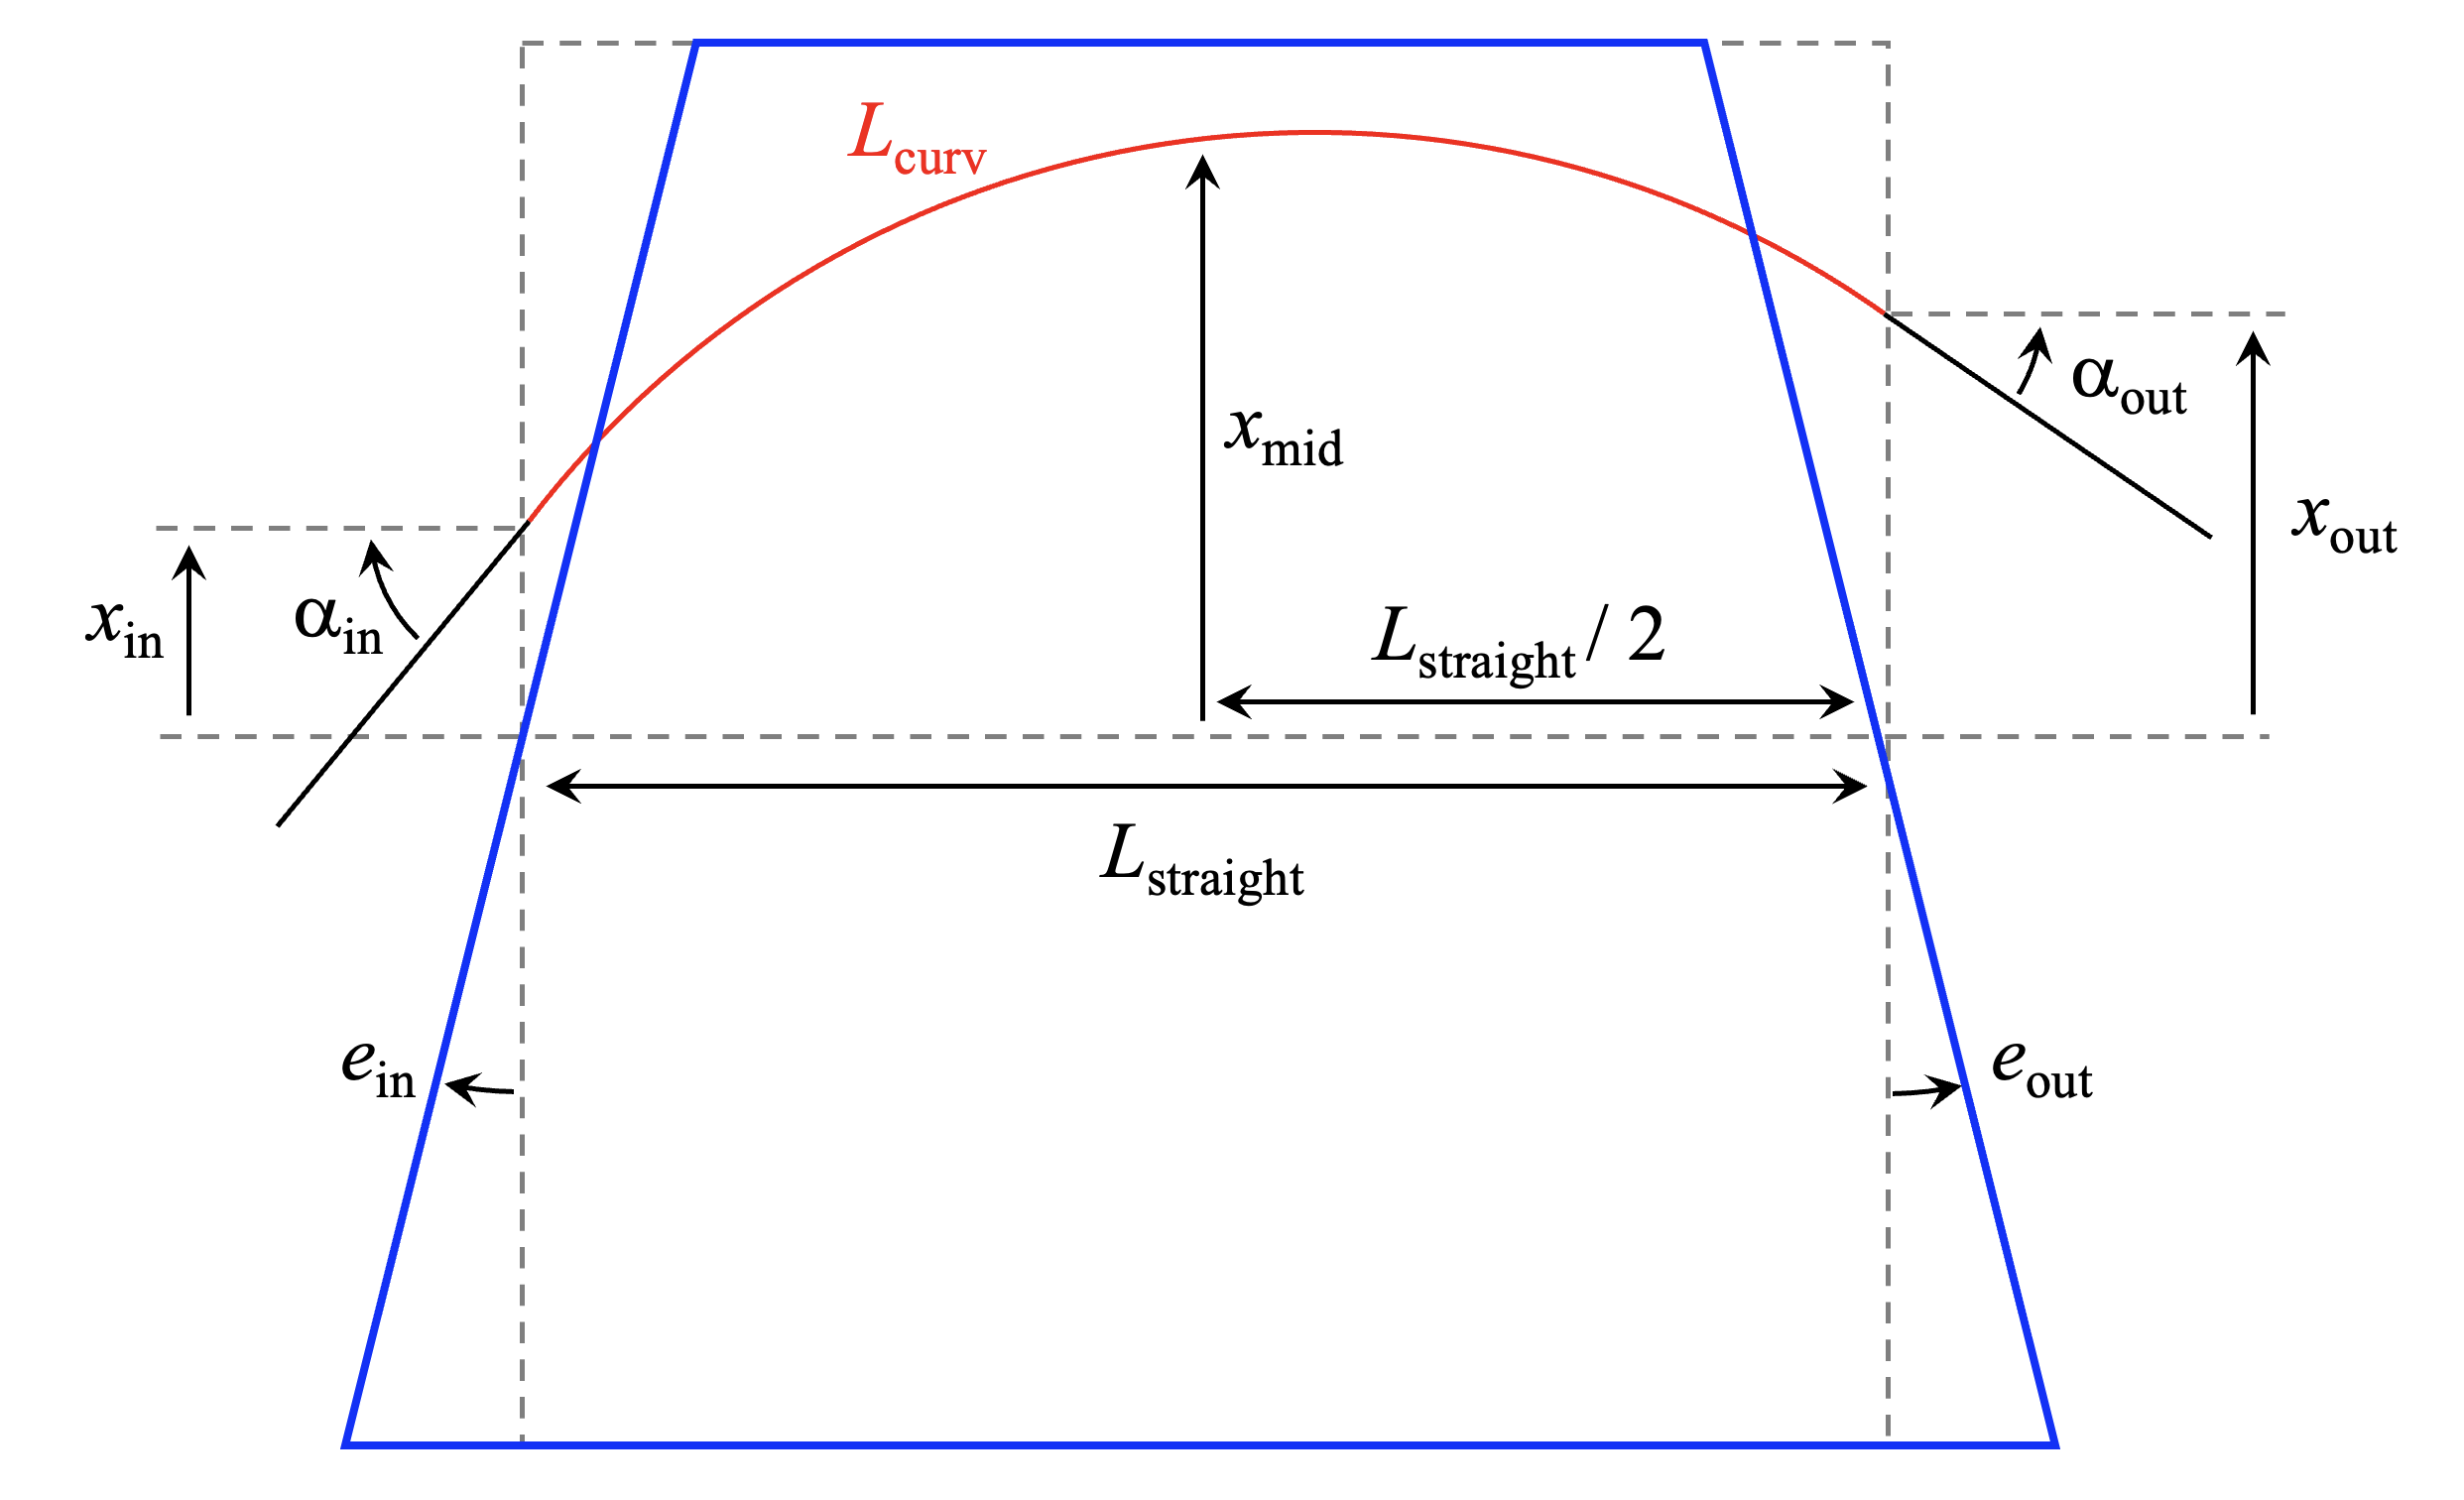
\includegraphics[height=0.40\textheight]{figures/rbend.png}
  \caption{Rectangular bend.\label{fig:rbend}}
\end{figure}

In the reference frame of the magnet body, for an on-momentum particle on the
reference trajectory we can write:
\begin{align}
&p_{x, \text{in}} = \sin(\alpha_\text{in}) \\
&p_{x, \text{out}} = -\sin(\alpha_\text{out})
\end{align}

Using Eq.~\eqref{eq:straight_bend_px} we can write:
\begin{equation}
  -\sin(\alpha_\text{out}) = \sin(\alpha_\text{in}) - h L_\text{straight}
\end{equation}
from which we can obtain the curvature of the reference trajectory:
\begin{equation}
  h = \frac{\sin(\alpha_\text{in}) + \sin(\alpha_\text{out})}{L_\text{straight}}
\end{equation}

Using Eqs.~\eqref{eq:straight_bend_x} and~\eqref{eq:straight_bend_px} we can write:
\begin{align}
  &p_{x,\text{mid}} = p_{x,\text{in}} - h L_\text{straight}/2 \label{eq:px_mid_in}\\
  &p_{x,\text{mid}} = p_{x,\text{out}} + h L_\text{straight}/2 \label{eq:px_mid_out}\\
  &x_\text{in} = x_\text{mid} - \frac{1}{h} \left(
    \sqrt{1 - p_{x,\text{mid}}^2} - \sqrt{1 - p_{x,\text{in}}^2} \right) \\
  &x_\text{out} = x_\text{mid} + \frac{1}{h} \left(
    \sqrt{1 - p_{x,\text{out}}^2} - \sqrt{1 - p_{x,\text{mid}}^2} \right)
\end{align}

Using Eq.~\eqref{eq:straight_bend_ell} we can write:
\begin{equation}
  L_\text{curv} = \frac{1}{h} \left(
    \sin^{-1} (p_{x,\text{out}}) - \sin^{-1} (p_{x,\text{in}}) \right)
    = \frac{\alpha_\text{in} + \alpha_\text{out}}{h}
    = \frac{\alpha}{h}
\end{equation}

In the special case of a sector bend ($\alpha_\text{diff} = 0$) we have, summing
Eqs.~\eqref{eq:px_mid_in} and \eqref{eq:px_mid_out}:
\begin{align}
&\alpha_\text{in} = \alpha_\text{out} = \frac{\alpha}{2} \\
&p_{x, \text{in}} = -p_{x, \text{out}} = \sin(\alpha/2) \\
&p_{x,\text{mid}} = 0 \\
&h = \frac{2 \sin(\alpha/2)}{L_\text{straight}} \\
&L_\text{curv} = \frac{\alpha}{h} = \frac{L_\text{straight}}{\text{sinc}(\alpha/2)}\\
&x_\text{in} = x_\text{out} = x_\text{mid} - \frac{1}{h} \left(
    1 - \cos(\alpha/2) \right)
\end{align}
The last gives the usual equation for the sagitta of a bending magnet.



\section{Expanded Bend-Quadrupole (also used for Quadrupole)}
\label{sec:expanded_bend_quadrupole}

Implemented in the \href{https://xsuite.readthedocs.io/en/latest/apireference.html#bend}{\underline{Bend}},
\href{https://xsuite.readthedocs.io/en/latest/apireference.html#rbend}{\underline{RBend}} and
\href{https://xsuite.readthedocs.io/en/latest/apireference.html#quadrupole}{\underline{Quadrupole}} elements,
for the ``mat-kick-mat'' model.
~\\
This map is ported from the MAD-X source code.
~\\

The following map is generated by the Hamiltonian:
\begin{equation}
  H_{M} = \frac{p_\tau}{\beta_0} +  \frac{1}{2}\frac{p_x^2 + p_y^2}{(1 + \delta)} + (K_0 -h)x + \frac{K_0hx^2}{2} + K_1 \frac{x^2-y^2}{2}
\end{equation}

We consider a particle with initial canonical coordinates
\[
(x,\, p_x,\, y,\, p_y,\, \zeta),
\]
relative momentum deviation $\delta$, velocity factor $\mathrm{rvv}=v/c$, and charge/sign factor $\chi$.
The element has length $L$, curvature $h$, and (input) strengths $K_0$ and $K_1$.

\subsection*{Definitions}

Define
\begin{align}
\delta_+ &\equiv 1+\delta, \\
x' &= \frac{p_x}{\delta_+}, \qquad
y' = \frac{p_y}{\delta_+}.
\end{align}

We introduce the momentum-scaled (effective) strengths
\begin{align}
\bar{K}_0 &= \frac{\chi\, K_0}{\delta_+}, \qquad
\bar{K}_1 = \frac{\chi\, K_1}{\delta_+},
\end{align}
and the corresponding focusing coefficients
\begin{align}
K_x &= \bar{K}_0\, h + \bar{K}_1, \\
K_y &= -\bar{K}_1 .
\end{align}

Auxiliary quantities:
\begin{align}
A &= -K_x x - \bar{K}_0 + h, \\
B &= x', \\
C &= -K_y y, \\
D &= y'.
\end{align}

\subsection*{Transport Functions}

For an element of length $L$, define
\[
(C_x,S_x)=
\begin{cases}
\left(\cos(\sqrt{K_x}L), \dfrac{\sin(\sqrt{K_x}L)}{\sqrt{K_x}}\right),
& K_x>0, \\[1em]
\left(\cosh(\sqrt{-K_x}L), \dfrac{\sinh(\sqrt{-K_x}L)}{\sqrt{-K_x}}\right),
& K_x<0, \\[1em]
(1,\,L), & K_x=0,
\end{cases}
\]
\[
(C_y,S_y)=
\begin{cases}
\left(\cos(\sqrt{K_y}L), \dfrac{\sin(\sqrt{K_y}L)}{\sqrt{K_y}}\right),
& K_y>0, \\[1em]
\left(\cosh(\sqrt{-K_y}L), \dfrac{\sinh(\sqrt{-K_y}L)}{\sqrt{-K_y}}\right),
& K_y<0, \\[1em]
(1,\,L), & K_y=0.
\end{cases}
\]

\subsection*{Transverse Map}

\paragraph{Positions}
\begin{align}
x_1 &= x C_x + x' S_x
+ \begin{cases}
\dfrac{(\bar{K}_0-h)(C_x-1)}{K_x}, & K_x\neq 0, \\[1em]
-\dfrac{1}{2}(\bar{K}_0-h)L^2, & K_x=0,
\end{cases}
\\
y_1 &= y C_y + y' S_y .
\end{align}

\paragraph{Momenta}
\begin{align}
p_{x1} &= \delta_+ \left(A S_x + B C_x\right), \\
p_{y1} &= \delta_+ \left(C S_y + D C_y\right).
\end{align}

\subsection*{Path Length}

Let $L_{\text{tot}}$ be the total path length traveled by the particle through the element.

\paragraph{Horizontal contribution}

For $K_x\neq 0$:
\begin{align}
L_{\text{tot}} &= L
- \frac{h\left[(C_x-1)x' + S_x A + L(\bar{K}_0-h)\right]}{K_x} \nonumber\\
&\quad + \frac{1}{2}\Bigg[
- \frac{A^2 C_x S_x}{2K_x}
+ \frac{B^2 C_x S_x}{2}
+ \frac{A^2 L}{2K_x}
+ \frac{B^2 L}{2} \nonumber\\
&\qquad\qquad
- \frac{A B C_x^2}{K_x}
+ \frac{A B}{K_x}
\Bigg].
\end{align}

For $K_x=0$:
\begin{equation}
L_{\text{tot}} =
L
+ \frac{hL}{6}\left(3Lx' + 6x - (\bar{K}_0-h)L^2\right)
+ \frac{1}{2}B^2 L .
\end{equation}

\paragraph{Vertical contribution}

For $K_y\neq 0$:
\begin{align}
L_{\text{tot}} \mathrel{+}= \frac{1}{2}\Bigg[
- \frac{C^2 C_y S_y}{2K_y}
+ \frac{D^2 C_y S_y}{2}
+ \frac{C^2 L}{2K_y}
+ \frac{D^2 L}{2} \nonumber\\
\qquad\qquad
- \frac{C D C_y^2}{K_y}
+ \frac{C D}{K_y}
\Bigg].
\end{align}

For $K_y=0$:
\begin{equation}
L_{\text{tot}} \mathrel{+}= \frac{1}{2}D^2 L .
\end{equation}

\subsection*{Longitudinal Map}

The longitudinal coordinate update is
\begin{equation}
\Delta\zeta = L - \frac{L_{\text{tot}}}{\mathrm{rvv}} .
\end{equation}

\subsection*{Final Map}

\begin{equation}
(x,p_x,y,p_y,\zeta)
\;\longrightarrow\;
(x_1,p_{x1},y_1,p_{y1},\zeta+\Delta\zeta),
\qquad
s \rightarrow s+L .
\end{equation}


\section{Exact path correction for mat-kick-mat}
\label{sec:mat_kick_mat_exact}

The \texttt{mat-kick-mat-exact} model extends \texttt{mat-kick-mat} for
straight magnets ($h=0$). Both propagate with the expanded bend--quadrupole
map $M$ described in Sec.~\ref{sec:expanded_bend_quadrupole}, retaining its
momentum dependence. The exact variant adds a correction depending only on momenta
that restores the square-root kinetic Hamiltonian omitted by the expansion
in transverse momentum. This follows the exact-model correction described by
Forest, Schmidt and McIntosh in the PTC report~\cite{ptc2002}, p.~69 and
Secs.~K.4.6--K.4.7, pp.~74--75.

With $p_z=\sqrt{(1+\delta)^2-p_x^2-p_y^2}$, the correction Hamiltonian is
\begin{equation}
  H_{Dc}=H_D-H_{De}
        =1+\delta-p_z-\frac{p_x^2+p_y^2}{2(1+\delta)}.
  \label{eq:mat_kick_mat_exact_correction}
\end{equation}
Thus, for $h=0$, adding $H_{Dc}$ to the expanded magnet Hamiltonian restores
the exact kinetic term while retaining the same magnetic multipole potential.
The factor $1/(1+\delta)$ in the expanded map is already retained exactly;
the correction restores the higher powers of transverse momentum.

Since $H_{Dc}$ has no position dependence, its map $C(\ell)$ over a signed
integration length $\ell$ leaves $p_x$, $p_y$ and $\delta$ unchanged. Define
\begin{equation}
  d=\ell\left(\frac{1}{p_z}-\frac{1}{1+\delta}\right).
\end{equation}
In Xtrack's longitudinal coordinate $\zeta$, the coordinate updates are
\begin{align}
  x &\leftarrow x+p_x d, \\
  y &\leftarrow y+p_y d, \\
  \zeta &\leftarrow \zeta+
    \frac{\beta_0}{\beta}\left(
       \frac{\ell(p_x^2+p_y^2)}{2(1+\delta)^2}-(1+\delta)d\right).
\end{align}
This correction does not advance $s$; that advance belongs to the propagation
map $M$.

For each multipole kick with integration length $\ell$, the implementation
applies $C(\ell/2)$, the multipole kick, and $C(\ell/2)$, in that order.
For example, one \texttt{uniform} step of length $\ell$ applies
\begin{equation}
  M(\ell/2)\;;\ C(\ell/2)\;;\ K(\ell)\;;\ C(\ell/2)\;;\ M(\ell/2).
\end{equation}
Here the operations are listed in tracking order; $K$ contains the multipole
terms not included in $M$. Other integrators use their own propagation and
kick weights, including signed lengths. An empty magnetic kick still requires
the correction: the two half-length maps combine into $C(\ell)$. With zero
field, the resulting map is an exact drift.

\section{Thin bend}

Implemented in the \href{https://xsuite.readthedocs.io/en/latest/apireference.html#multipole}{\underline{Multipole element}}.
~\\

In a curvilinear reference system with a constant curvature $h$ in the
horizontal plane a uniform magnetic field can be derived from the vector potential:
\begin{align}
  A_x & = 0, & A_y & = 0, & A_s & =
  - B_y \left(x-\frac{h x^2}{2 (1+h x)}\right).
\end{align}

With the following normalization, $K_0=\frac{q_0}{p} B_y$ is the inverse of the bending
radius of the reference particle.

The exact and expanded Hamiltonians for a horizontal bending magnet are (eq. 2.12 in
\cite{barber87})
\begin{align}
  H &= \frac{p_\tau}{\beta_0}
       - (1+h x)\sqrt{(1+\delta)^2 -p_x^2 - p_y^2}
       + \chi K_0 \left( x + \frac{h x^2}{2} \right)  \\
    &\simeq   \frac{p_\tau}{\beta_0}
    + \frac{1}{2}\frac{p_x^2+p_y^2}{1+\delta}
  - (1+h x) (1+\delta) + \chi K_0 \left( x + \frac{h x^2}{2} \right)
\end{align}


The map for a thin dipole kick (horizontal or vertical) from the expanded Hamiltonian is
(eq. 4.12 in \cite{heinemann95}):
\begin{align}
  p_x &\leftarrow p_x - \chi K_0 L + h L (1 + \delta)  - \chi K_0  h x L\\
  \tau &\leftarrow \tau - \frac{h x}{\beta}  L.
\end{align}



\section{Thin Multipole}

Implemented in the \href{https://xsuite.readthedocs.io/en/latest/apireference.html#multipole}{\underline{Multipole element}}.
~\\

Multipolar components are defined according to the definition in Sec.~\ref{sec:multipole_expansion}.


A thin multipole models the effect of the field by taking the limit of the integration
length going to zero while keeping constant the integrated strength. The Hamiltonian is:
\begin{align}
  H= \delta(s) \chi L \Re\left[\sum_{n=0} \frac{1}{(n+1)!}(K_n + i\hat K_n) (x+iy)^{n+1} \right].
\end{align}

The corresponding map is:
\begin{align}
  p_x &\leftarrow p_x - \chi L\cdot\Re\left[\sum_{n=0} \frac{1}{n!} (K_n + i\hat K_n) (x+iy)^n \right], \\
  p_y &\leftarrow p_y + \chi L\cdot\Im\left[\sum_{n=0} \frac{1}{n!} (K_n + i\hat K_n) (x+iy)^n \right],
\end{align}
where $L$ is the length of the modeled multipole element.

The other coordinates ($x$, $y$, $\delta$, $\zeta$) remain unchanged.

\section{Dipole fringe field} \label{sec:DipoleFringeField}

A dipole magnet bends a particle through its approximately uniform body
field. Near an entrance or exit, the field changes between the body value
and the external value. This transition is the \emph{fringe field}. The
transition also produces a longitudinal magnetic-field component away from
the mid-plane, and that component can change the vertical momentum.
An edge can therefore focus or defocus the vertical motion even when the
uniform dipole body has no vertical focusing in Cartesian coordinates.

This section derives that effect starting from the Lorentz force. We first
obtain the linear vertical kick of an ideal hard edge, then calculate the
leading correction for a field transition of finite width. We next introduce
a Hamiltonian description to extend the model to nonzero vertical slope and
construct a consistent map of all phase-space coordinates. Finally, we
explain the effective-angle form used in tracking, derive its corrected
coefficient, and give the generating function and tracking derivatives.

The dipole fringe field map used in Xsuite is based on
Ref.~\cite{forest-fringe-1}; additional background is given in
Refs.~\cite{silke_cap, silke_fringe}. The derivation below states the
assumptions and intermediate steps needed here. In particular, the
finite-width calculation is perturbative to second order in field strength.
The resulting symplectic tracking model extends that calculation; it is not
an exact solution for every fringe profile or every transverse amplitude.

\subsection{Geometry, coordinates and magnetic field}

We use a right-handed Cartesian frame $(x,y,s)$, with $s$ normal to the pole
face, $y$ vertical, and $x$ horizontal. The nominal edge is at $s=0$.
The mid-plane is $y=0$. A mid-plane particle trajectory lies in the
$(x,s)$ plane; to calculate its vertical focusing we consider a small
vertical displacement and momentum about that trajectory. A particle exactly
at $y=p_y=0$ receives no vertical kick.

We derive an entrance edge: the field rises from zero before the magnet
to its body value after the edge. Magnetic-field and incidence-angle signs
are defined in this fixed frame. The derivation assumes the particle has
the reference charge and mass, and there is no electric field. In the
implementation, a particle of different charge or mass sees the body field
$K_0$ multiplied by the rigidity factor $\chi=(q/q_0)(m_0/m)$ introduced
with the particle coordinates; all formulas below then apply with
$K_0\to\chi K_0$. Normalize mechanical
momenta by the reference momentum, so that
\begin{align}
 p&=1+\delta,\label{eq:fringe_coordinates}\\
 p_s&=\sqrt{p^2-p_x^2-p_y^2},\\
 x'&=\frac{dx}{ds}=\frac{p_x}{p_s},\\
 y'&=\frac{dy}{ds}=\frac{p_y}{p_s}.
\end{align}
The positive square root selects forward motion, $p_s>0$. The magnetic
field changes the direction of the mechanical momentum but not its
magnitude $p$. The slopes $x',y'$ are ratios of momentum components; they
are not angles measured in radians. Canonical momenta will be introduced
explicitly when we construct the Hamiltonian.

Let $s_-$ and $s_+$ denote positions before and after the field transition.
In the distributed-field derivation, arguments specify where a quantity is
evaluated: $p_x(s)$ and $y(s)$ vary along the trajectory, whereas
$p_x(s_-)$ and $y(s_-)$ denote their incoming values. We write the
mechanical slopes as $x_p(s)=p_x(s)/p_s(s)$ and
$y_p(s)=p_y(s)/p_s(s)$. These are particle quantities, not parameters of
a fixed reference trajectory. Normal incidence is not assumed.
For a thin map at the nominal plane, we instead use unadorned symbols
for incoming coordinates and a subscript $f$ for outgoing coordinates;
this convention will also be used when inverting the map.

Let $b(s)$ be the mid-plane vertical magnetic field divided by the reference
magnetic rigidity $(B\rho)_0$. It has units of inverse length. For an
entrance fringe, $b(s_-)=0$ and $b(s_+)=K_0$, where the endpoints lie outside
the transition and $K_0$ is the signed normalized body field. We assume the
ideal dipole field is independent of $x$, with $B_x=0$ and mid-plane
symmetry. In the current-free aperture, Maxwell's equations imply
\begin{equation}
 \partial_y B_s=\partial_s B_y,\qquad
 \partial_y B_y=-\partial_s B_s.
\end{equation}
Since $B_s(s,0)=0$ by symmetry, the first relation gives
$B_s/(B\rho)_0=y b'(s)+O(y^3)$. Inserting this in the second relation gives
$B_y/(B\rho)_0=b(s)-y^2b''(s)/2+O(y^4)$. Continuing in powers of $y$ yields
\begin{align}
 \frac{B_y}{(B\rho)_0}&=b(s)-\frac{y^2}{2}b''(s)+\cdots,
 \label{eq:fringe_fields}\\
 \frac{B_s}{(B\rho)_0}&=y b'(s)-\frac{y^3}{6}b'''(s)+\cdots.
\end{align}
Primes denote derivatives with respect to $s$. Thus a changing vertical
field necessarily produces a longitudinal field away from the mid-plane.
This longitudinal component is the origin of the vertical edge kick.

\subsection{Lorentz equations near the mid-plane}

Writing the Lorentz force with $s$ as the independent variable gives
\begin{equation}
 \frac{d\boldsymbol p}{ds}
 =\left(\frac{p_x}{p_s},\frac{p_y}{p_s},1\right)
   \mathbin{\times}\frac{\boldsymbol B}{(B\rho)_0},
\end{equation}
where $\boldsymbol p=(p_x,p_y,p_s)$ is the normalized mechanical momentum.
In particular,
\begin{align}
 \frac{dp_x}{ds}
 &=\frac{p_y}{p_s}\frac{B_s}{(B\rho)_0}
   -\frac{B_y}{(B\rho)_0},
 \label{eq:fringe_lorentz_px}\\
 \frac{dp_y}{ds}
 &=\frac{B_x}{(B\rho)_0}
   -\frac{p_x}{p_s}\frac{B_s}{(B\rho)_0}.
 \label{eq:fringe_lorentz_py}
\end{align}
Linearize in the vertical displacement and momentum, keeping the horizontal
angle exact. The product $p_y B_s$ is second order in vertical amplitude,
and $p_y^2$ does not enter $p_s$ at linear order. Using the field expansion
above gives
\begin{align}
 \frac{dp_x}{ds}&=-b(s),
 \label{eq:fringe_ode_px}\\
 \frac{dy}{ds}&=\frac{p_y}{p_s},
 \label{eq:fringe_ode_y}\\
 \frac{dp_y}{ds}&=-\frac{p_x}{p_s}\,b'(s)y,
 \label{eq:fringe_ode_py}\\
 p_s&=\sqrt{p^2-p_x^2}.
 \label{eq:fringe_longitudinal_momentum}
\end{align}
These equations are linear in the vertical variables but need not be
expanded in field strength; they can also be integrated numerically for a
specified smooth profile $b(s)$.

\subsection{Hard-edge limit and linear vertical focusing}

A hard edge idealizes the transition as having zero longitudinal width
while keeping the field jump $K_0$ fixed. To derive its kick without
multiplying singular fields, first use the linear vertical equations for a
smooth transition of width $L$, and then take $L\to0$.
Equation~\eqref{eq:fringe_ode_px} gives
\begin{equation}
 p_x(s_+)-p_x(s_-)=-\int_{s_-}^{s_+}b(s)\,ds=O(K_0L).
\end{equation}
Thus the horizontal momentum change across the shrinking transition
vanishes, so the horizontal slope tends to $x_p(s_-)$.
The vertical position remains continuous. Integrating
Eq.~\eqref{eq:fringe_ode_y} over a vanishing length gives
$y(s_+)\to y(s_-)$ for finite vertical momentum.
The vertical momentum change, however, need not vanish, because the
integral of $b'$ is the fixed field jump:
\begin{equation}
 \int_{s_-}^{s_+}b'(s)\,ds=b(s_+)-b(s_-)=K_0.
\end{equation}
Integrating Eq.~\eqref{eq:fringe_ode_py} in this limit therefore gives
\begin{align}
 \Delta p_y
 &=-x_p(s_-)y(s_-)\int_{s_-}^{s_+}b'(s)\,ds\\
 &=-K_0x_p(s_-)\,y(s_-).
 \label{eq:fringe_hard_edge_kick}
\end{align}
This is the hard-edge vertical focusing law in the pole-face frame. Its
linear map is
\begin{equation}
 \begin{pmatrix}y(s_+)\\p_y(s_+)\end{pmatrix}
 =\begin{pmatrix}1&0\\-K_0x_p(s_-)&1\end{pmatrix}
  \begin{pmatrix}y(s_-)\\p_y(s_-)\end{pmatrix}.
\end{equation}
It holds for any small incoming vertical momentum, including zero: at the
linear order in the vertical variables used here, an incoming $p_y$ does not
alter the coefficient. The dependence on the vertical slope found in the
Hamiltonian treatment below, the factor $1/(1+y_p^2)$ in
Eq.~\eqref{eq:fringe_u}, is quadratic in $y_p$ and therefore lies beyond this
linearization.
When $K_0x_p(s_-)$ is positive, a positive displacement receives a negative momentum
kick, directed toward the mid-plane: the edge focuses. Reversing the sign
of $K_0x_p(s_-)$ makes it defocusing. At normal incidence, $x_p(s_-)=0$, this
hard-edge vertical kick vanishes.

The horizontal velocity couples to the longitudinal fringe field in the
Lorentz force. Although the transition width tends to zero, that
longitudinal field grows in proportion to $b'$, so its integrated vertical
impulse stays finite. This is why a hard edge can produce a kick.
The derivation is a limit of the linearized equations; it does not assert
that the off-mid-plane field of an infinitely sharp edge is regular.

The coefficient $K_0x_p(s_-)$ has units of inverse length. At fixed incidence
angle it has no explicit dependence on $p$ when acting on the normalized
momentum $p_y$. The slope change does have momentum dependence:
\begin{equation}
 \Delta y'=\frac{\Delta p_y}{p_s(s_-)}
           =-\frac{K_0x_p(s_-)}{p_s(s_-)}y(s_-).
\end{equation}
This distinction matters when comparing formulas written in slopes and in
normalized momenta. For a falling field transition, the same integration
uses its signed field jump $-K_0$ instead of $K_0$, with the slope
$x_p(s_-)$ measured in the frame whose $s$ axis is normal to the exit face.
The treatment of the exit face in the implementation is described in
Section~\ref{sec:fringe_exit_face}.

\subsection{Finite-width correction for zero incoming vertical slope}

We take $p_y(s_-)=0$, hence zero incoming vertical slope, and retain a
small incoming vertical displacement $y(s_-)$. The mid-plane itself is
$y=0$; a trajectory confined to it has both $y=0$ and $p_y=0$ and receives
no vertical kick. Here we calculate the linear response to a displacement
from that trajectory. The coefficient multiplying $y(s_-)$ in the
resulting momentum kick is the vertical focusing coefficient. The vertical
momentum generally becomes nonzero as the particle crosses the fringe.

For a finite transition width, $p_x/p_s$ and $y$ change while the particle
crosses the fringe. Their first-order changes modify the vertical force
and give the leading correction to Eq.~\eqref{eq:fringe_hard_edge_kick}.
We now compute that correction to second order in field strength.

An equivalent thin fringe replaces the distributed transition by a map at
its nominal plane. The ordinary drift before that plane and uniform-field
bend after it are factored out. A uniform Cartesian dipole does not change
$p_y$, so its removal leaves the vertical momentum kick unchanged.

The field-profile dependence of the correction can be expressed through
\begin{equation}
 I=\int_{s_-}^{s_+}b(s)\bigl(K_0-b(s)\bigr)\,ds.
\end{equation}
The integrand vanishes both before the entrance and in the uniform body,
so only the transition contributes. For a hard edge $I\to0$; a finite
transition generally gives a nonzero value. In tracking, this quantity is
specified by the full magnet gap $g=2\,\texttt{hgap}$ and the dimensionless
fringe integral $F=\texttt{fint}$:
\begin{equation}
 F=\frac{1}{gK_0^2}\int_{s_-}^{s_+}
          b(s)\bigl(K_0-b(s)\bigr)\,ds,\qquad I=gK_0^2F.
 \label{eq:fringe_integral}
\end{equation}
The gap $g$ is a transverse distance, not the longitudinal transition width
$L$. The product $gF$ encodes the profile integral; specifying it does not
specify the complete field profile. For a fixed profile shape and width,
$I$ is proportional to $K_0^2$.

To extract the finite-width correction analytically, specify the incoming
displacement $y(s_-)$ and take $p_y(s_-)=0$. Introduce the accumulated
normalized field integral
\begin{equation}
 \mathcal{I}(s)=\int_{s_-}^{s}b(\sigma)\,d\sigma,\qquad
 p_x(s)=p_x(s_-)-\mathcal{I}(s).
\end{equation}
The second relation follows by integrating
Eq.~\eqref{eq:fringe_ode_px}, $dp_x/ds=-b(s)$, from $s_-$ to $s$,
with the incoming value $p_x(s_-)$.
The integral $\mathcal{I}(s)$ is distinct from the quadratic
fringe integral $I$ in Eq.~\eqref{eq:fringe_integral}.
Evaluating Eq.~\eqref{eq:fringe_longitudinal_momentum} at the entrance gives
the incoming longitudinal momentum; the corresponding horizontal slope is
\begin{equation}
 p_s(s_-)=\sqrt{p^2-p_x(s_-)^2},\qquad x_p(s_-)=\frac{p_x(s_-)}{p_s(s_-)}.
\end{equation}
The magnetic field preserves the total momentum $p$, but both $p_x(s)$ and
$p_s(s)$ vary along the trajectory. Using
Eq.~\eqref{eq:fringe_longitudinal_momentum} to express their ratio as a
function of $p_x(s)$, define, at fixed $p$,
\begin{equation}
 f(a)=\frac{a}{\sqrt{p^2-a^2}},\qquad
 \frac{p_x(s)}{p_s(s)}=f\bigl(p_x(s_-)-\mathcal{I}(s)\bigr).
\end{equation}
Differentiating the numerator and denominator gives
\begin{align}
 f'(a)
 &=\frac{1}{\sqrt{p^2-a^2}}
   +\frac{a^2}{(p^2-a^2)^{3/2}}\\
 &=\frac{p^2}{(p^2-a^2)^{3/2}}.
\end{align}
The first-order Taylor expansion about the incoming momentum $p_x(s_-)$ is
therefore
\begin{align}
 f\bigl(p_x(s_-)-\mathcal{I}(s)\bigr)
 &=f(p_x(s_-))-\mathcal{I}(s)f'(p_x(s_-))
   +O\bigl(\mathcal{I}(s)^2\bigr)\\
 &=x_p(s_-)-\frac{p^2}{p_s(s_-)^3}\mathcal{I}(s)
   +O\bigl(\mathcal{I}(s)^2\bigr).
\end{align}
For a fixed fringe shape and length, $b(s)=K_0\widehat b(s)$ with
$\widehat b(s)$ independent of $K_0$, so $\mathcal{I}(s)$ is proportional to
$K_0$. Holding $p$ and $p_x(s_-)$ fixed while expanding in the field strength
therefore gives
\begin{equation}
 \frac{p_x(s)}{p_s(s)}
 =x_p(s_-)-\frac{p^2}{p_s(s_-)^3}\mathcal{I}(s)+O(K_0^2).
\end{equation}
Since $b'(s)$ is already first order in $K_0$, the first-order vertical
force uses the zero-field values $p_x/p_s=x_p(s_-)$ and $y=y(s_-)$ in
Eq.~\eqref{eq:fringe_ode_py}. Integrating from $s_-$, where $p_y=0$ and
$b=0$, gives
\begin{equation}
 p_y^{(1)}(s)
 =-x_p(s_-)y(s_-)\int_{s_-}^{s}b'(\sigma)\,d\sigma
 =-x_p(s_-)b(s)y(s_-).
\end{equation}
To obtain the first-order change in position, insert this result into
Eq.~\eqref{eq:fringe_ode_y} and use the zero-field denominator $p_s(s_-)$:
\begin{equation}
 y^{(1)}(s)=\int_{s_-}^{s}\frac{p_y^{(1)}(\sigma)}{p_s(s_-)}\,d\sigma
 =-\frac{x_p(s_-)y(s_-)}{p_s(s_-)}\mathcal{I}(s).
\end{equation}
The superscript $(1)$ denotes the first-order change; the position itself
is $y(s)=y(s_-)+y^{(1)}(s)+O(K_0^2)$.
Substituting both corrections back into Eq.~\eqref{eq:fringe_ode_py},
\begin{align}
 \frac{dp_y}{ds}
 &=-x_p(s_-) b'(s)y(s_-)\nonumber\\
 &\quad+\left(\frac{p^2}{p_s(s_-)^3}+\frac{x_p(s_-)^2}{p_s(s_-)}\right)\mathcal{I}(s)b'(s)y(s_-)
   +O(K_0^3 y(s_-)),\\
 \int \mathcal{I}(s)b'(s)\,ds
 &=[\mathcal{I}(s)b(s)]_{s_-}^{s_+}-\int b(s)^2\,ds
   =\int b(s)\bigl(K_0-b(s)\bigr)\,ds=I.
\end{align}
The resulting kick coefficient is therefore
\begin{equation}
 \frac{\Delta p_y}{y(s_-)}
 =-K_0x_p(s_-)+I\frac{1+2x_p(s_-)^2}{p_s(s_-)}+O(K_0^3).
\label{eq:fringe_midplane_kick}
\end{equation}
The first term is the hard-edge focusing. The second is the leading correction
due to the finite field transition. At fixed incoming slope, the finite-gap correction scales as $1/p$,
since $p_s(s_-)=p/\sqrt{1+x_p(s_-)^2}$. Its slope dependence must be
preserved when correcting the momentum dependence.

\subsection{Momentum-dependent coefficient of the generating function}

Our aim is to determine the momentum-dependent focusing coefficient $\Phi$
of an equivalent thin fringe kick, written at the retained linear vertical
order as
\begin{equation}
 \Delta p_y=-\Phi(p_x,p_y,\delta)Y.
\end{equation}
Here $Y$ is the vertical position extrapolated to the nominal fringe plane
along an unperturbed drift; its precise definition is given below.
The preceding section obtained the kick for zero incoming vertical momentum.
We now seek the coefficient used in the operator model of
Ref.~\cite{forest-fringe-1}, which also describes nonzero incoming vertical
momentum. We construct the field Hamiltonian, remove the ordinary drift
motion, and calculate the first- and second-order contributions in the
field strength. The second-order calculation retains the terms needed for
linear mid-plane focusing; their unexpanded momentum dependence defines the
model's extension away from the mid-plane. The resulting $\Phi$ provides
the coefficient that the generating-function model must reproduce to this
order, rather than a description of every nonlinear fringe effect.

We first specify the vector potential and the momentum convention used in
the Hamiltonian. The normalized vector potential is
\begin{equation}
 \mathbf a=\frac{\mathbf A}{(B\rho)_0}.
\end{equation}
Choose its components as
\begin{align}
 a_x&=a(s,y),\label{eq:fringe_ax}\\
 a_y&=0,\label{eq:fringe_ay}\\
 a_s&=-x b(s).\label{eq:fringe_as}
\end{align}
The scalar $a(s,y)$ therefore denotes the horizontal component of the
normalized vector potential. Taking the curl in the Cartesian frame gives
\begin{align}
 \frac{B_x}{(B\rho)_0}
 &=\partial_y a_s-\partial_s a_y=0,\\
 \frac{B_y}{(B\rho)_0}
 &=\partial_s a_x-\partial_x a_s=b(s)+\partial_s a(s,y),
 \label{eq:fringe_curl_by}\\
 \frac{B_s}{(B\rho)_0}
 &=\partial_x a_y-\partial_y a_x=-\partial_y a(s,y).
 \label{eq:fringe_curl_bs}
\end{align}
Thus $a_s$ supplies the mid-plane vertical field, while $a_x$ supplies its
off-mid-plane corrections and the longitudinal fringe field.

To determine $a(s,y)$, impose Maxwell's equation
$\partial_s B_y=\partial_y B_s$ in the current-free aperture. Substituting
Eqs.~\eqref{eq:fringe_curl_by} and \eqref{eq:fringe_curl_bs} gives
\begin{equation}
 b'(s)+\partial_s^2 a+\partial_y^2 a=0.
 \label{eq:fringe_potential_pde}
\end{equation}
Mid-plane symmetry allows an even series in $y$; choose $a(s,0)=0$ and write
\begin{equation}
 a(s,y)=c_2(s)y^2+c_4(s)y^4+c_6(s)y^6+\cdots.
\end{equation}
Matching powers of $y$ in Eq.~\eqref{eq:fringe_potential_pde} yields
\begin{align}
 b'+2c_2&=0,\\
 c_2''+12c_4&=0,\\
 c_{2n}''+(2n+2)(2n+1)c_{2n+2}&=0\qquad(n\geq1).
\end{align}
Consequently $c_2=-b'/2$, $c_4=b'''/24$, and in general
\begin{equation}
 a(s,y)=\sum_{n=1}^{\infty}
 \frac{(-1)^n b^{(2n-1)}(s)}{(2n)!}\,y^{2n}
 =-\frac{b'(s)}{2}y^2+\frac{b'''(s)}{24}y^4-\cdots.
 \label{eq:fringe_ax_series}
\end{equation}
Here $b^{(n)}$ denotes the $n$-th derivative with respect to $s$.
As a check, substituting this series into
Eqs.~\eqref{eq:fringe_curl_by} and \eqref{eq:fringe_curl_bs} gives
\begin{align}
 \frac{B_y}{(B\rho)_0}
 &=b(s)-\frac{b''(s)}2y^2+\frac{b^{(4)}(s)}{24}y^4-\cdots,\\
 \frac{B_s}{(B\rho)_0}
 &=b'(s)y-\frac{b'''(s)}6y^3+\frac{b^{(5)}(s)}{120}y^5-\cdots,
\end{align}
which reproduce the field expansion in Eq.~\eqref{eq:fringe_fields}.

We now use canonical momenta in the Hamiltonian. Their relation to the
normalized mechanical momenta is
\begin{equation}
 p_x^{\mathrm{mech}}=p_x-a_x,\qquad
 p_y^{\mathrm{mech}}=p_y-a_y,\qquad
 p_s^{\mathrm{can}}=p_s^{\mathrm{mech}}+a_s.
\end{equation}
The preceding Lorentz-equation derivation used mechanical transverse
momenta. Since $a_x=O(y^2)$ and $a_y=0$, the transverse canonical and
mechanical momenta agree to the linear vertical order used there.
The symbol $p$ continues to denote the conserved total mechanical momentum.
For forward motion its longitudinal component is
\begin{equation}
 p_s^{\mathrm{mech}}
 =\sqrt{p^2-(p_x-a_x)^2-(p_y-a_y)^2}.
\end{equation}
At fixed energy, using $s$ as the independent variable gives the reduced
Hamiltonian $H=-p_s^{\mathrm{can}}=-p_s^{\mathrm{mech}}-a_s$.
Inserting the chosen vector potential therefore gives
\begin{equation}
 H=-\sqrt{p^2-(p_x-a)^2-p_y^2}+b(s)x.
 \label{eq:fringe_hamiltonian}
\end{equation}
To identify the perturbation to the drift Hamiltonian, define
\begin{equation}
 H_0=-\sqrt{p^2-p_x^2-p_y^2},\qquad
 p_s=\sqrt{p^2-p_x^2-p_y^2}.
\end{equation}
For this unperturbed drift, denote the particle's slopes by
$x_p=p_x/p_s$ and $y_p=p_y/p_s$. They are functions of the particle's
canonical momenta, not fixed slopes of a reference trajectory. They remain
constant along a free drift because its momenta are constant, but change
when the incoming momenta are varied. In particular, their momentum
derivatives must be retained in the tracking map.

Inside the magnetic field, these drift slopes must be distinguished from
the actual mechanical slopes. For the chosen gauge, the latter are
\begin{equation}
 \frac{dx}{ds}=\frac{p_x-a(s,y)}{p_s^{\mathrm{mech}}},\qquad
 \frac{dy}{ds}=\frac{p_y}{p_s^{\mathrm{mech}}}.
\end{equation}
At a field-free entrance, $x_p$ evaluated at the incoming momenta equals
the incoming mechanical slope $x_p(s_-)$ used above.
Expanding
Eq.~\eqref{eq:fringe_hamiltonian} to first order in $a$ gives
\begin{equation}
 H=H_0+b(s)x-\frac{p_x}{p_s}a(s,y)+O(a^2).
\end{equation}
We denote the part of $H-H_0$ that is first order in field strength by $V$:
\begin{equation}
 V(s,x,y,p_x,p_y)=b(s)x-x_pa(s,y),\qquad
 H=H_0+V+O(K_0^2).
 \label{eq:fringe_physical_perturbation}
\end{equation}
Both $b$ and $a$ are proportional to $K_0$ for a fixed field profile.
At this stage $V$ retains the full vertical-position series of $a(s,y)$;
the expansion in field strength has not truncated that series.

The drift interaction frame removes the motion generated by $H_0$ before
expanding in the fringe perturbation. To define it explicitly, Hamilton's
equations for the unperturbed drift are
\begin{align}
 \frac{dx}{ds}&=\frac{\partial H_0}{\partial p_x}
              =\frac{p_x}{p_s}=x_p,\label{eq:fringe_drift_x}\\
 \frac{dy}{ds}&=\frac{\partial H_0}{\partial p_y}
              =\frac{p_y}{p_s}=y_p,\label{eq:fringe_drift_y}\\
 \frac{dp_x}{ds}&=-\frac{\partial H_0}{\partial x}=0,\\
 \frac{dp_y}{ds}&=-\frac{\partial H_0}{\partial y}=0.
\end{align}
The slopes are therefore constant under this drift. Choose a reference
plane $s=s_*$ and introduce coordinates $X,Y$ by
\begin{align}
 X&=x-(s-s_*)x_p,\label{eq:fringe_interaction_x}\\
 Y&=y-(s-s_*)y_p.\label{eq:fringe_interaction_y}
\end{align}
These are the positions obtained by extrapolating the instantaneous
phase-space point back to $s_*$ along a free drift; the transformation leaves
the momenta unchanged. In the absence of the field perturbation, $X,Y$ are
constant. With the fringe present, they evolve because of that perturbation.
Thus this change of coordinates does not assume that the actual trajectory
through the fringe is a straight line.

The transformation is the inverse Hamiltonian flow of $H_0$ and is
canonical. Its explicit dependence on $s$ subtracts $H_0$ from the
transformed Hamiltonian, leaving
\begin{equation}
 H_I(s,X,Y,p_x,p_y)
 =\left.(H-H_0)\right|_{x=X+(s-s_*)x_p,\;y=Y+(s-s_*)y_p}.
\end{equation}
The subscript $I$ denotes the interaction frame. Define $V_I$ to be the
same first-order perturbation $V$, evaluated at the physical positions
corresponding to $X,Y$:
\begin{equation}
 V_I(s,X,Y,p_x,p_y)
 =V\bigl(s,X+(s-s_*)x_p,Y+(s-s_*)y_p,p_x,p_y\bigr).
\end{equation}
Substitution of Eq.~\eqref{eq:fringe_physical_perturbation} gives
\begin{equation}
 V_I=b(s)\bigl[X+(s-s_*)x_p\bigr]
     -x_p a\bigl(s,Y+(s-s_*)y_p\bigr).
 \label{eq:fringe_interaction_perturbation}
\end{equation}
Thus $H_I=V_I+O(K_0^2)$: $V_I$ is the first-order part of the
interaction-frame Hamiltonian, not its full expression to all field orders.
This explains the positive shifts in the arguments: the field perturbation
must be evaluated at the physical position corresponding to $X,Y$ at $s$.
Choose the nominal fringe plane as the origin, $s_*=0$. The physical
positions entering $V$ are then $X+s x_p$ and $Y+s y_p$.
We retain $X,Y$ for the interaction-frame positions and $x_p,y_p$
for the unperturbed drift slopes throughout the derivation.

To obtain the first-order vertical kick, use Hamilton's equation
$dp_y/ds=-\partial H_I/\partial Y$ and retain $V_I$, the part first order
in field strength. Integrating with the interaction-frame coordinates and
momenta held at their unperturbed values gives
\begin{equation}
 \Delta p_y^{(1)}
 =-\frac{\partial}{\partial Y}\int V_I\,ds.
 \label{eq:fringe_first_order_kick_integral}
\end{equation}
The term $b(s)(X+s x_p)$ has no $Y$-dependence, so it contributes no
vertical kick. Since $x_p$ is independent of $Y$, this reduces to
\begin{equation}
 \Delta p_y^{(1)}
 =x_p\frac{\partial}{\partial Y}
   \int a(s,Y+s y_p)\,ds.
 \label{eq:fringe_first_order_a_integral}
\end{equation}
The vector-potential integral is therefore an intermediate step toward
the kick: its derivative with respect to $Y$, multiplied by $x_p$,
gives the momentum change. To evaluate it, consider the $n$-th term of
the series in Eq.~\eqref{eq:fringe_ax_series}. Integrating by parts
$2n-2$ times gives
\begin{align}
 &\int_{s_-}^{s_+}
 \frac{(-1)^n b^{(2n-1)}(s)}{(2n)!}(Y+s y_p)^{2n}\,ds\nonumber\\
 &\qquad=\frac{(-1)^n y_p^{2n-2}}{2}
       \int_{s_-}^{s_+}b'(s)(Y+s y_p)^2\,ds.
\end{align}
All boundary terms contain derivatives of $b$ that vanish outside the
transition. The remaining polynomial derivative supplies the factor
$(2n)!/2$ and the power $y_p^{2n-2}$. Expanding the square gives
\begin{equation}
 \int b'(s)(Y+s y_p)^2\,ds
 =K_0Y^2+2Yy_p\int b'(s)\,s\,ds+y_p^2\int b'(s)\,s^2\,ds.
\end{equation}
The last term does not depend on $Y$ and drops out of the derivative in
Eq.~\eqref{eq:fringe_first_order_a_integral}. The middle term is removed by
the choice of the nominal plane: we place $s=0$ at the centroid of $b'$,
\begin{equation}
 \int_{s_-}^{s_+}b'(s)\,s\,ds=0,
 \label{eq:fringe_edge_position}
\end{equation}
which is the midpoint of a transition that is antisymmetric about its
centre, such as the hyperbolic-tangent profile used below. This convention
fixes where the thin map is placed; it does not require the transition
width to vanish. The part of the integral that contributes to the kick is
therefore $K_0Y^2$ for any width, and summing over $n$ gives
\begin{align}
 \int a(s,Y+s y_p)\,ds
 &\doteq\frac{K_0Y^2}{2}\sum_{n=1}^{\infty}(-1)^n y_p^{2n-2}
   =-\frac{K_0Y^2}{2(1+y_p^2)},
\end{align}
where $\doteq$ denotes equality up to terms independent of $Y$.
The sum is first obtained where the geometric series converges and then used
as its rational continuation. Substituting this result into
Eq.~\eqref{eq:fringe_first_order_a_integral} and differentiating at fixed
momenta gives
\begin{equation}
 \Delta p_y^{(1)}
 =x_p\frac{\partial}{\partial Y}
   \left[-\frac{K_0Y^2}{2(1+y_p^2)}\right]
 =-K_0uY,
\end{equation}
where the dimensionless slope combination $u$ is defined as
\begin{equation}
 u=\frac{x_p}{1+y_p^2}.
 \label{eq:fringe_u}
\end{equation}
This is an auxiliary function of the two unperturbed drift slopes, not an
independent coordinate. It is the factor entering the first-order vertical
kick, $\Delta p_y^{(1)}=-K_0uY$, and thus gives the first-order focusing
coefficient $\Phi^{(1)}=K_0u$. On the mid-plane, $y_p=0$, it reduces to
$u=x_p$. For nonzero vertical
slope, its denominator accounts for the vertical-slope dependence in this
fringe model. This first-order result reduces to the hard-edge mid-plane
kick derived directly from the Lorentz force in
Eq.~\eqref{eq:fringe_hard_edge_kick}.

To calculate the contribution $C=O(K_0^2)$ to the focusing coefficient
$\Phi=K_0u-C$, we use the ordered second-order perturbation expansion.
First expand the vertical-position dependence of $V_I$ explicitly.
Using $a(s,y)=-b'(s)y^2/2+b'''(s)y^4/24-\cdots$ in
Eq.~\eqref{eq:fringe_interaction_perturbation}, with $s_*=0$, gives
\begin{align}
 V_I={}&b(s)(X+s x_p)
       +\frac{x_p}{2}b'(s)(Y+s y_p)^2\nonumber\\
      &-\frac{x_p}{24}b'''(s)(Y+s y_p)^4+\cdots.
\end{align}
We denote by $W$ the truncation of $V_I$ that retains the horizontal term
and the leading quadratic vertical term:
\begin{equation}
 W(s)=b(s)(X+s x_p)+\frac{x_p}{2}b'(s)(Y+s y_p)^2.
 \label{eq:fringe_truncated_perturbation}
\end{equation}
Here $W(s)$ abbreviates $W(s,X,Y,p_x,p_y)$; it still depends on the
transverse coordinates and momenta. It is not an additional physical
interaction or a second-order Hamiltonian. Like $V_I$, $W$ is first order
in $K_0$, but it omits the fourth and higher powers of the physical vertical
position $Y+s y_p$.
Its two successive actions in the ordered expansion produce the
second-order contribution $C$. Thus ``second order'' refers to the field
strength, whereas ``quadratic'' refers to the vertical position.
This truncation is part of the approximation used for linear mid-plane
focusing; keeping the remaining momentum dependence unexpanded does not
recover the omitted nonlinear terms.
Define the transverse Poisson bracket by
\begin{equation}
 \{f,h\}=f_Xh_{p_x}-f_{p_x}h_X+f_Yh_{p_y}-f_{p_y}h_Y.
\end{equation}
To see why a double integral appears, consider the motion generated by
$W$ and write the interaction-frame phase-space coordinates as
$\mathbf z=(X,Y,p_x,p_y)$. Hamilton's equations are
$dz_j/ds=\{z_j,W(s)\}$, in particular
$dp_y/ds=\{p_y,W(s)\}=-\partial W(s)/\partial Y$.
At first order, the force is evaluated at the unperturbed phase-space point,
so only one integration is needed. The first-order change accumulated by
the time the particle reaches $s_1$ is
\begin{equation}
 z_j^{(1)}(s_1)=\int_{s_-}^{s_1}\{z_j,W(s_2)\}\,ds_2.
 \label{eq:fringe_first_order_trajectory}
\end{equation}
At second order, the vertical force at $s_1$ must account for this earlier
change. To make the expansion explicit, denote the vertical momentum-change
rate generated by $W$ by
\begin{equation}
 \mathcal F_y(s,\mathbf z)=\{p_y,W(s,\mathbf z)\}.
\end{equation}
Write the perturbed trajectory as
\begin{equation}
 \mathbf z(s_1)=\mathbf z^{(0)}+\mathbf z^{(1)}(s_1)+O(K_0^2).
\end{equation}
Here $\mathbf z^{(0)}$ is the constant unperturbed interaction-frame point,
and $\mathbf z^{(1)}$ is its first-order change, not the full trajectory.
A Taylor expansion of the force about $\mathbf z^{(0)}$ gives
\begin{align}
 \mathcal F_y(s_1,\mathbf z(s_1))
 ={}&\mathcal F_y(s_1,\mathbf z^{(0)})\nonumber\\
 &+\sum_j\left.
       \frac{\partial\mathcal F_y(s_1,\mathbf z)}{\partial z_j}
       \right|_{\mathbf z^{(0)}}z_j^{(1)}(s_1)+O(K_0^3).
\end{align}
The first term is the first-order force. In the second term,
$\partial\mathcal F_y/\partial z_j=O(K_0)$ and $z_j^{(1)}=O(K_0)$,
so their product is second order in field strength. This contribution is
therefore
\begin{equation}
 \left(\frac{dp_y}{ds_1}\right)^{(2)}
 =\sum_j\frac{\partial\mathcal F_y(s_1)}{\partial z_j}
                  z_j^{(1)}(s_1).
\end{equation}
From here on, all brackets and derivatives are evaluated at
$\mathbf z^{(0)}$ unless stated otherwise. Inserting
Eq.~\eqref{eq:fringe_first_order_trajectory} gives
\begin{equation}
 \left(\frac{dp_y}{ds_1}\right)^{(2)}
 =\int_{s_-}^{s_1}\sum_j
   \frac{\partial\mathcal F_y(s_1)}{\partial z_j}
   \{z_j,W(s_2)\}\,ds_2.
\end{equation}
The sum over the four coordinates is a Poisson bracket. Explicitly, writing
$W_2=W(s_2)$ and suppressing the argument $s_1$ of $\mathcal F_y$,
\begin{align}
 \sum_j\frac{\partial\mathcal F_y}{\partial z_j}\{z_j,W_2\}
 ={}&\frac{\partial\mathcal F_y}{\partial X}\frac{\partial W_2}{\partial p_x}
    +\frac{\partial\mathcal F_y}{\partial Y}\frac{\partial W_2}{\partial p_y}
       \nonumber\\
   &-\frac{\partial\mathcal F_y}{\partial p_x}\frac{\partial W_2}{\partial X}
    -\frac{\partial\mathcal F_y}{\partial p_y}\frac{\partial W_2}{\partial Y}
       \nonumber\\
 ={}&\{\mathcal F_y,W_2\}.
\end{align}
Restoring $\mathcal F_y(s_1)=\{p_y,W(s_1)\}$ then yields
\begin{align}
 \left(\frac{dp_y}{ds_1}\right)^{(2)}
 &=\int_{s_-}^{s_1}
   \bigl\{\{p_y,W(s_1)\},W(s_2)\bigr\}\,ds_2.
\end{align}
The inner bracket is the vertical force at $s_1$; the outer bracket gives
its change due to the earlier interaction at $s_2$.
Integrating the force over the later
position $s_1$ therefore produces the ordered double integral
\begin{equation}
 \Delta p_y^{(2)}
 =\int_{s_-}^{s_+}ds_1\int_{s_-}^{s_1}ds_2\,
   \bigl\{\{p_y,W(s_1)\},W(s_2)\bigr\}.
 \label{eq:fringe_ordered_second_order_kick}
\end{equation}
The inner integration sums the earlier perturbations at $s_2$; the outer
one sums their effects on the force at the later position $s_1$.
The limit $s_2<s_1$ enforces this ordering. Each occurrence of $W$ supplies
one power of $K_0$, so this contribution is second order in field strength.
It is the Hamiltonian counterpart of substituting the first-order trajectory
changes back into the Lorentz force in the preceding derivation.

By antisymmetry of the Poisson bracket,
\begin{equation}
 \bigl\{\{p_y,W(s_1)\},W(s_2)\bigr\}
 =\bigl\{W(s_2),\{W(s_1),p_y\}\bigr\}.
\end{equation}
In this integrand, the terms retained for linear mid-plane focusing are
\begin{equation}
 Y\left[b(s_2)b'(s_1)\{X,x_p\}
 +x_p^2 b'(s_2)b'(s_1)(s_1-s_2)\{Y,y_p\}\right].
\end{equation}
For example, the first term comes from the bracket of $b(s_2)X$ with
$x_p b'(s_1)Y$. The second comes from the vertical-position and
vertical-momentum derivatives of the two quadratic terms in $W$.
Terms containing additional explicit powers of the vertical displacement or
vertical slope are not retained in this step. Keeping the momentum
derivatives $\{X,x_p\}$ and $\{Y,y_p\}$ unexpanded defines the conventional
extension away from the mid-plane; it does not restore the other discarded
terms. Integrating the retained expression over the ordered pair
$(s_2,s_1)$ in Eq.~\eqref{eq:fringe_ordered_second_order_kick} gives
$\Delta p_y^{(2)}=CY$, where
\begin{equation}
 C=\{X,x_p\}J_0+x_p^2\{Y,y_p\}(J_{10}-J_{01}),
\end{equation}
where
\begin{align}
 J_0&=\int_{s_-}^{s_+} b'(s_1)\,ds_1\int_{s_-}^{s_1}b(s_2)\,ds_2=I,\\
 J_{10}-J_{01}
 &=\int_{s_-}^{s_+} b'(s_1)\,ds_1\int_{s_-}^{s_1}
       b'(s_2)(s_1-s_2)\,ds_2=I.
\end{align}
For the second identity, the inner integral equals
$\int_{s_-}^{s_1}b(s_2)\,ds_2$ by integration by parts, since $b(s_-)=0$.
The remaining momentum derivatives are explicit:
\begin{align}
 \{X,x_p\}=\frac{\partial (p_x/p_s)}{\partial p_x}
 &=\frac{p^2-p_y^2}{p_s^3}=\frac{1+x_p^2}{p_s},\\
 \{Y,y_p\}=\frac{\partial (p_y/p_s)}{\partial p_y}
 &=\frac{p^2-p_x^2}{p_s^3}=\frac{1+y_p^2}{p_s}.
\end{align}
Combining the first- and second-order kicks gives
$\Delta p_y=-K_0uY+CY=-\Phi Y$ at the retained order.
Consequently, writing $A=1+x_p^2(2+y_p^2)$, the coefficient to be matched is
\begin{equation}
 \Phi=K_0u-C=K_0u-gK_0^2F\frac{A}{p_s}.
\label{eq:fringe_phi_second_order}
\end{equation}
This is Eq.~(34) of Ref.~\cite{forest-fringe-1} in the present notation.
At $p_y=0$, it reproduces the independent derivation in
Eq.~\eqref{eq:fringe_midplane_kick}, with $\Delta p_y=-\Phi Y$.
For general vertical slopes it specifies the chosen operator approximation;
matching it does not establish an exact finite-width field map to all
transverse orders.

\subsection{Constructing the corrected tangent form}

Denote by $\psi(p_x,p_y,\delta)$ the momentum-dependent focusing coefficient
used in the tracking model. At the retained linear vertical order, its
kick is $\Delta p_y=-\psi Y$. Thus $\psi$ has units of inverse length;
it is a focusing strength, not an angle. It will also supply the coefficient
of the quadratic vertical term in the generating function below.
The coefficient $\Phi$ derived in Eq.~\eqref{eq:fringe_phi_second_order}
is the perturbative result through second order in field strength. We
require the model coefficient to reproduce that result:
\begin{equation}
 \psi=\Phi+O(K_0^3).
\end{equation}
Using distinct symbols distinguishes the derived expansion $\Phi$ from
the unexpanded tracking-model expression $\psi$.

To connect the slope-based result to the existing effective-angle model,
introduce the signed incoming mid-plane incidence angle $e$, measured
from the $s$ axis toward $+x$. For forward motion,
\begin{equation}
 p_x=p\sin e,\qquad p_s=p\cos e,\qquad x_p=\tan e,
 \qquad p_y=0.
 \label{eq:fringe_incidence_angle}
\end{equation}
Here the momenta are incoming values. At the field-free entrance,
$x_p=x_p(s_-)$, connecting to the mechanical slope used above.
Equation~\eqref{eq:fringe_hard_edge_kick} therefore has
focusing coefficient $K_0\tan e$. The finite-width result in
Eq.~\eqref{eq:fringe_midplane_kick} can likewise be written
\begin{equation}
 \frac{\Delta p_y}{y(s_-)}=-K_0\tan e
 +\frac{gK_0^2F}{p}\frac{1+\sin^2e}{\cos^3e}+O(K_0^3).
 \label{eq:fringe_angle_kick}
\end{equation}
The existing tracking model expresses the finite-fringe correction as a
shift of an effective edge angle. On the mid-plane this means replacing
$e$ by $e-\epsilon$, giving a coefficient $K_0\tan(e-\epsilon)$.
For nonzero vertical slope, the first-order result is $K_0u$, so the
corresponding effective angle is $\arctan u$: it equals $e$ on the
mid-plane for forward motion, but in general it is a function of both
slopes, not simply the geometric incidence angle.

We retain this form of the existing model and determine the angle shift
by requiring agreement with the derived focusing coefficient through
second order in field strength. For the model coefficient $\psi$, write
\begin{equation}
 \psi=K_0\tan\bigl(\arctan u-\epsilon\bigr),\qquad
 \epsilon=O(K_0).
\end{equation}
Expand the outer tangent, keeping the momenta fixed:
\begin{align}
 \tan(\arctan u-\epsilon)
 &=u-(1+u^2)\epsilon+O(\epsilon^2),\\
 \psi&=K_0u-K_0(1+u^2)\epsilon+O(K_0^3).
\end{align}
Agreement with Eq.~\eqref{eq:fringe_phi_second_order} requires
\begin{equation}
 \epsilon=gK_0F\frac{A}{p_s(1+u^2)}.
\end{equation}
Thus the corrected expression used in the map is\footnote{%
In the notation used here, the original PTC expression in Eq.~(37) of
Forest's fringe note, Ref.~\cite{forest-fringe-1}, is
\[
 \psi_{\mathrm{PTC}}=K_0\tan\!\left[\arctan u-gK_0F A p_s\right],
 \qquad A=1+x_p^2(2+y_p^2).
\]
Expanding the outer tangent gives
$\psi_{\mathrm{PTC}}=K_0u-gK_0^2F A p_s(1+u^2)+O(K_0^3)$,
whereas Eq.~(34) of that note requires
$K_0u-gK_0^2F A/p_s$ through second order. Thus Eqs.~(34) and (37)
do not agree to that order in general, contrary to the statement following
Eq.~(37). They agree for $\delta=0$ and $p_y=0$, where
$p_s^2(1+u^2)=1$. On the mid-plane at fixed incidence angle, the original
PTC second-order correction scales as $p=1+\delta$, instead of the required
$1/p$. The factor $1/[p_s(1+u^2)]$ in Eq.~\eqref{eq:fringe_psi}
restores agreement with Eq.~(34).}
\begin{equation}
 \boxed{\displaystyle
 \psi=K_0\tan\left[\arctan u-
       gK_0F\frac{1+x_p^2(2+y_p^2)}{p_s(1+u^2)}\right],
 \qquad u=\frac{x_p}{1+y_p^2}.}
\label{eq:fringe_psi}
\end{equation}
The tangent form is a model choice beyond the calculated order. The
unexpanded tangent includes terms of order $K_0^3$ and higher whose accuracy
has not been established by this matching. It is not required for
symplecticity: that follows from using a single generating function
consistently for all coordinates, as described below.

On the mid-plane, $y_p=0$, so
\begin{equation}
 \frac{1}{p_s(1+u^2)}=\frac{p_s}{p_s^2+p_x^2}
 =\frac{p_s}{(1+\delta)^2}=\frac{\cos e}{1+\delta}.
\end{equation}
The mid-plane angle shift is therefore
$\epsilon=gK_0F(1+\sin^2e)/[(1+\delta)\cos e]$, the expression of SLAC-75
and MAD-X divided by $1+\delta$.

\subsection{Generating function and forward map}

The thin map acts at the nominal plane $s=0$, where
Eqs.~\eqref{eq:fringe_interaction_x} and \eqref{eq:fringe_interaction_y}
give $X=x$ and $Y=y$. We write its incoming and outgoing physical positions
as $(x,y)$ and $(x_f,y_f)$. The coefficient $\psi$ retains the slope
notation $x_p=p_x/p_s$ and $y_p=p_y/p_s$, evaluated at the incoming
canonical momenta.

A generating function is a scalar function whose derivatives define a
canonical, and hence symplectic, transformation. Here we use a mixed
generating function: its independent arguments are the incoming momenta
and outgoing positions. With the longitudinal canonical pair
$(\ell,-\delta)$, the defining relations are
\begin{align}
 x&=\frac{\partial\mathcal G}{\partial p_x},&
 p_{x,f}&=\frac{\partial\mathcal G}{\partial x_f},\\
 y&=\frac{\partial\mathcal G}{\partial p_y},&
 p_{y,f}&=\frac{\partial\mathcal G}{\partial y_f},\\
 \ell&=-\frac{\partial\mathcal G}{\partial\delta},&
 \delta_f&=-\frac{\partial\mathcal G}{\partial\ell_f}.
\end{align}
The function $p_xx_f+p_yy_f-\delta\ell_f$ gives the identity map.
Adding $-\psi y_f^2/2$ generates the desired vertical kick, together with
the position and longitudinal changes required by the momentum dependence
of $\psi$. We first construct this map alone; the additional cubic kick
present in the implementation is described separately in
Section~\ref{sec:fringe_cubic_extension}.
We construct a symplectic thin-fringe map using the focusing coefficient
$\psi$ defined in Eq.~\eqref{eq:fringe_psi}. To generate the vertical kick
$p_{y,f}=p_y-\psi y_f$, we choose the mixed generating function
\begin{equation}
 \mathcal G=p_xx_f+p_yy_f-\delta\ell_f
             -\frac12\psi(p_x,p_y,\delta)y_f^2.
 \label{eq:fringe_generating_function}
\end{equation}
The first three terms, $p_xx_f+p_yy_f-\delta\ell_f$, generate the identity
map: without the last term, all positions and momenta remain unchanged.
The last term introduces the fringe kick and its associated coordinate changes.
Differentiating the generating function with respect to $p_y$ and $y_f$ gives
\begin{align}
 y&=\frac{\partial\mathcal G}{\partial p_y}
   =y_f-\frac12\psi_{p_y}y_f^2,\\
 p_{y,f}&=\frac{\partial\mathcal G}{\partial y_f}
         =p_y-\psi y_f.
\end{align}
Solving the quadratic equation for $y_f$ using the root continuous at $y=0$
gives the forward map:
\begin{equation}
\begin{aligned}
p_s &= \sqrt{(1+\delta)^2 - p_x^2 - p_y^2}\\
x_f &= x + \frac{1}{2} \frac{\partial \psi}{\partial p_x} y_f^2 \\
p_{x,f} &= p_x \\
y_f &= \frac{2y}{1 + \sqrt{1 - 2 \frac{\partial \psi}{\partial p_y} y}} \\
p_{y,f} &= p_y - \psi y_f \\
\ell_f &= \ell - \frac{1}{2} \frac{\partial \psi}{\partial \delta} y_f^2 \\
\delta_f &= \delta
\end{aligned}
\label{eq:fringe_map}
\end{equation}
All derivatives are evaluated at the incoming momenta. The map is symplectic where this branch
of the generating function is real and invertible; that property alone does
not make the finite-width approximation exact.

\subsection{Additional cubic kick in the implementation}
\label{sec:fringe_cubic_extension}

Xtrack also applies a cubic vertical kick. The same term appears in the
\href{https://github.com/MethodicalAcceleratorDesign/MAD-X/blob/master/libs/ptc/src/Sh_def_kind.f90}{PTC dipole-fringe implementation}.
This term is separate from the focusing coefficient $\psi$ derived above.
Its coefficient, in the present notation, is
\begin{equation}
 c_3=\frac{K_0^2}{36Fg(1+\delta)}.
 \label{eq:fringe_cubic_coefficient}
\end{equation}
The same cubic coefficient is documented for the SAD soft-edge model in
the Bmad Reference Manual~\cite{Sagan:BmadManual}.

We now derive it independently at normal incidence for a specified smooth
field profile.

Take incoming mechanical momenta $p_x(s_-)=p_y(s_-)=0$ and vertical displacement
$y(s_-)$. Retain second order in field strength and third order in $y(s_-)$.
Starting from $p_x(s_-)=0$, the horizontal Lorentz equation,
Eq.~\eqref{eq:fringe_lorentz_px}, generates $p_x=O(K_0)$.
The vertical Lorentz equation, Eq.~\eqref{eq:fringe_lorentz_py} with $B_x=0$,
contains the product $p_x B_s$. Since $B_s=O(K_0)$, the vertical force
starts at $O(K_0^2)$. With incoming $p_y=0$, the vertical momentum is
therefore $O(K_0^2)$, and Eq.~\eqref{eq:fringe_ode_y}, $dy/ds=p_y/p_s$,
shows that the vertical displacement change also starts at that order.
In the force calculation at that order we can use $y(s)=y(s_-)$
and $p_s=p=1+\delta$.

It is essential to retain the off-mid-plane correction to $B_y$, as well
as the cubic term of $B_s$:
\begin{align}
 \frac{B_y}{(B\rho)_0}&=b(s)-\frac{y(s_-)^2}{2}b''(s)+O(y(s_-)^4),\\
 \frac{B_s}{(B\rho)_0}&=y(s_-)b'(s)-\frac{y(s_-)^3}{6}b'''(s)+O(y(s_-)^5).
\end{align}
Using mechanical momenta explicitly, the horizontal Lorentz equation
at first order in field strength gives
\begin{align}
 \frac{dp_x^{\mathrm{mech}}}{ds}
 &=-b(s)+\frac{y(s_-)^2}{2}b''(s)+O(y(s_-)^4),\\
 p_x^{\mathrm{mech}}(s)
 &=-\mathcal I(s)+\frac{y(s_-)^2}{2}b'(s)+O(y(s_-)^4),
 \qquad \mathcal I(s)=\int_{s_-}^{s}b(\sigma)\,d\sigma.
\end{align}
Here $b'(s_-)=0$; the omitted field-strength orders are not needed below.
Substituting this momentum into
$dp_y^{\mathrm{mech}}/ds=-(p_x^{\mathrm{mech}}/p_s)B_s/(B\rho)_0$
gives, to second order in field strength,
\begin{equation}
 \frac{dp_y^{\mathrm{mech}}}{ds}
 =\frac{\mathcal I(s)b'(s)}{p}y(s_-)
  -\frac{y(s_-)^3}{p}\left[
       \frac{\mathcal I(s)b'''(s)}{6}
       +\frac{[b'(s)]^2}{2}\right]+O(y(s_-)^5).
\end{equation}
Define the additional field-profile integral
\begin{equation}
 J=\int_{s_-}^{s_+}[b'(s)]^2\,ds.
 \label{eq:fringe_cubic_profile_integral}
\end{equation}
With $b'$ and $b''$ vanishing at the endpoints, integration by parts twice
gives
\begin{align}
 \int_{s_-}^{s_+}\mathcal I(s)b'''(s)\,ds
 &=[\mathcal I b'']_{s_-}^{s_+}-\int_{s_-}^{s_+}b(s)b''(s)\,ds\\
 &=-[b b']_{s_-}^{s_+}+\int_{s_-}^{s_+}[b'(s)]^2\,ds=J.
\end{align}
Using also $\int\mathcal I b'\,ds=I$, we obtain the kick at the retained
orders:
\begin{equation}
 \Delta p_y=\frac{I}{p}y(s_-)-\frac{2J}{3p}y(s_-)^3.
 \label{eq:fringe_cubic_lorentz_kick}
\end{equation}
The first term is the normal-incidence finite-width focusing term already
derived. To represent the cubic term in the thin map, we add the quartic
term $-c_3y_f^4$ to the generating function. Its derivative with respect
to the outgoing position $y_f$ gives the additional momentum kick
\begin{equation}
 \Delta p_y^{\mathrm{cubic}}
 =\frac{\partial(-c_3y_f^4)}{\partial y_f}=-4c_3y_f^3.
\end{equation}
At the order retained here, $y_f$ can be replaced by the incoming
displacement $y(s_-)$: their difference is second order in field strength,
while $c_3$ is already second order. Matching this kick to the cubic
term in Eq.~\eqref{eq:fringe_cubic_lorentz_kick} therefore gives
\begin{equation}
 c_3=\frac{J}{6p}.
 \label{eq:fringe_cubic_general_coefficient}
\end{equation}
The uniform-body map factored out of the fringe does not
change $p_y$, so the derived momentum kick also applies to the equivalent
thin map.

For a hyperbolic-tangent field profile with length scale $d>0$,
\begin{equation}
 b(s)=\frac{K_0}{2}\left[1+\tanh(s/d)\right],\qquad
 b'(s)=\frac{K_0}{2d}\operatorname{sech}^2(s/d).
\end{equation}
Integrating over the full transition, with $r=s/d$, gives
\begin{align}
 gF&=\frac{d}{4}\int_{-\infty}^{\infty}\operatorname{sech}^2r\,dr
       =\frac d2,\\
 J&=\frac{K_0^2}{4d}\int_{-\infty}^{\infty}\operatorname{sech}^4r\,dr
       =\frac{K_0^2}{3d}.
\end{align}
For the second integral, $t=\tanh r$ gives
$\int_{-1}^{1}(1-t^2)\,dt=4/3$. Equation~\eqref{eq:fringe_cubic_general_coefficient}
therefore becomes
\begin{equation}
 c_3=\frac{K_0^2}{18dp}
     =\frac{K_0^2}{36gF(1+\delta)}.
\end{equation}

For a general profile, $J=\int[b']^2ds$ is not determined by
$gF=\int b(K_0-b)ds/K_0^2$. The implemented expression effectively sets
$J=K_0^2/(6gF)$, as for the hyperbolic-tangent profile. It should therefore
not be interpreted as a universal coefficient for arbitrary fringe shapes.
Nor does the normal-incidence calculation establish the complete cubic
map at finite incidence angle or nonzero incoming vertical slope.
Ref.~\cite{forest-fringe-1}, Eqs.~(21)--(22), likewise identifies additional
nonlinear profile integrals but leaves their further study aside.
For the hyperbolic-tangent profile, the cubic coefficient grows as $1/d$
when the transition narrows. The displacement expansion requires
$|y(s_-)|\ll d$, so its validity is not uniform in the limit $d\to0$ at fixed
nonzero $y(s_-)$. This nonlinear limit must be distinguished from the
linearized hard-edge calculation above.

To include the implemented cubic kick in a symplectic map, augment
Eq.~\eqref{eq:fringe_generating_function} by a quartic term:
\begin{equation}
 \mathcal G_{\mathrm{extended}}=\mathcal G-c_3y_f^4.
\end{equation}
Differentiating with respect to $y_f$ produces the extra kick
$-4c_3y_f^3$. Since $c_3$ depends on $\delta$, its derivative also produces
a longitudinal-coordinate change. The two modified lines of
Eq.~\eqref{eq:fringe_map} are
\begin{align}
 p_{y,f}&=p_y-\psi y_f-4c_3y_f^3,
 \label{eq:fringe_extended_py}\\
 \ell_f&=\ell-\frac12\psi_\delta y_f^2
                   +\frac{c_3}{1+\delta}y_f^4.
 \label{eq:fringe_extended_map}
\end{align}
Here $\partial c_3/\partial\delta=-c_3/(1+\delta)$; the quartic longitudinal
term must accompany the cubic vertical kick. All other lines of the map,
including the expression determining $y_f$, are unchanged because $c_3$
does not depend on $p_x$ or $p_y$. In the tracking coordinate $\zeta$, the
extended longitudinal update is
\begin{equation}
 \zeta_f=\zeta+\frac{\beta_0}{2}\psi_{p_\tau}y_f^2
              -\beta_0c_3\frac{T}{p^2}y_f^4.
\end{equation}
This extension does not change the linear vertical focusing about $y=0$.

\subsection{Complete generating function and forward map}
Combining the focusing coefficient $\psi$ from Eq.~\eqref{eq:fringe_psi}
with the cubic coefficient $c_3$ from
Eq.~\eqref{eq:fringe_cubic_coefficient}, the complete generating function is
\begin{equation}
 \mathcal G_{\mathrm{extended}}
 =p_xx_f+p_yy_f-\delta\ell_f
  -\frac12\psi(p_x,p_y,\delta)y_f^2-c_3(\delta)y_f^4.
 \label{eq:fringe_complete_generating_function}
\end{equation}
Its forward map is
\begin{equation}
\begin{aligned}
 y_f&=\frac{2y}{1+\sqrt{1-2\psi_{p_y}y}},\\
 x_f&=x+\frac12\psi_{p_x}y_f^2,\\
 p_{x,f}&=p_x,\\
 p_{y,f}&=p_y-\psi y_f-4c_3y_f^3,\\
 \ell_f&=\ell-\frac12\psi_\delta y_f^2
                  +\frac{c_3}{1+\delta}y_f^4,\\
 \delta_f&=\delta.
\end{aligned}
\label{eq:fringe_complete_map}
\end{equation}
All coefficients and momentum derivatives are evaluated at the incoming
momenta. Equivalently, in the longitudinal tracking coordinates,
\begin{equation}
 \zeta_f=\zeta+\frac{\beta_0}{2}\psi_{p_\tau}y_f^2
              -\beta_0c_3\frac{T}{p^2}y_f^4,
 \qquad p_{\tau,f}=p_\tau,
\end{equation}
where $p=1+\delta$ and $T=1/\beta_0+p_\tau$. The next section details
the derivatives of $\psi$; the additional coefficient satisfies
$\partial c_3/\partial\delta=-c_3/p$ and has no dependence on $p_x$ or $p_y$.

\subsection{Derivatives used in tracking}

The forward map in Eq.~\eqref{eq:fringe_map} needs three derivatives of
$\psi$: $\partial\psi/\partial p_x$ determines the horizontal position
change, $\partial\psi/\partial p_y$ enters the equation for $y_f$, and
$\partial\psi/\partial\delta$ determines the longitudinal change. All are
evaluated at the incoming momenta, holding the other incoming momenta and
the magnet parameters $K_0,g,F$ fixed.

The complication is that Eq.~\eqref{eq:fringe_psi} is expressed through
slopes and longitudinal momentum, rather than directly through
$(p_x,p_y,\delta)$. Their dependence is
\begin{equation}
 p=1+\delta,\qquad p_s=\sqrt{p^2-p_x^2-p_y^2},\qquad
 x_p=\frac{p_x}{p_s},\qquad y_p=\frac{p_y}{p_s}.
 \label{eq:fringe_derivative_inputs}
\end{equation}
Changing $p_x$, for example, changes not only $x_p$ but also $p_s$
and $y_p$. We must include all three changes. We do this in two stages:
first differentiate the focusing expression with respect to its three
intermediate arguments, then apply the chain rule to the incoming momenta.

\paragraph{1. Write the focusing coefficient as a composite function.}
For the intermediate differentiation, write
\begin{equation}
 \psi(p_x,p_y,\delta)
 =\Psi\bigl(x_p(p_x,p_y,\delta),
            y_p(p_x,p_y,\delta),p_s(p_x,p_y,\delta)\bigr).
\end{equation}
The capital $\Psi$ denotes the same focusing expression, with its three
arguments temporarily treated as independent. It is not an additional
physical coefficient. To organize its evaluation, define
\begin{align}
 u&=\frac{x_p}{1+y_p^2},\\
 A&=1+x_p^2(2+y_p^2),\\
 R&=\frac{A}{1+u^2},\\
 \phi&=\arctan u-\frac{gK_0F}{p_s}R,\\
 \Psi&=K_0\tan\phi.
 \label{eq:fringe_derivative_composition}
\end{align}
Here $u$ is the slope combination already introduced, $A$ is the numerator
of the finite-gap correction, and $R$ includes its compensating denominator
$1+u^2$. The angle $\phi$ is the argument of the outer tangent. These
quantities are only intermediate steps in evaluating Eq.~\eqref{eq:fringe_psi}.

\paragraph{2. Differentiate with respect to the intermediate arguments.}
In this paragraph a subscript denotes a partial derivative with respect to
that argument, holding the other two intermediate arguments fixed.
For example, $u_{x_p}=\partial u/\partial x_p$ at fixed
$y_p$ and $p_s$. Direct differentiation gives
\begin{align}
 u_{x_p}&=\frac{1}{1+y_p^2},\\
 u_{y_p}&=-\frac{2x_py_p}{(1+y_p^2)^2},\\
 A_{x_p}&=2x_p(2+y_p^2),\\
 A_{y_p}&=2x_p^2y_p.
\end{align}
For either slope argument $a\in\{x_p,y_p\}$, the quotient rule gives
\begin{equation}
 R_a=\frac{A_a(1+u^2)-A\,2u u_a}{(1+u^2)^2}
     =\frac{A_a-2uR u_a}{1+u^2}.
\end{equation}
Differentiating the arctangent and then the outer tangent gives
\begin{align}
 \phi_a&=\frac{u_a}{1+u^2}-\frac{gK_0F}{p_s}R_a,\\
 \Psi_a&=K_0\sec^2\phi\,\phi_a
 =K_0\sec^2\phi\left(\frac{u_a}{1+u^2}
                         -\frac{gK_0F}{p_s}R_a\right).
 \label{eq:fringe_auxiliary_slope_derivative}
\end{align}
For the remaining argument $p_s$, the slopes are held fixed, so $u$ and
$R$ are constant. Only the explicit factor $1/p_s$ changes:
\begin{equation}
 \Psi_{p_s}=K_0\sec^2\phi\,\frac{gK_0F R}{p_s^2}.
 \label{eq:fringe_auxiliary_ps_derivative}
\end{equation}
These three derivatives describe changes in the intermediate arguments.
We next convert them to derivatives with respect to the incoming momenta.

\paragraph{3. Differentiate the slopes and longitudinal momentum.}
From Eq.~\eqref{eq:fringe_derivative_inputs}, differentiation of the square
root gives
\begin{equation}
 \frac{\partial p_s}{\partial p_x}=-\frac{p_x}{p_s}=-x_p,\qquad
 \frac{\partial p_s}{\partial p_y}=-y_p,\qquad
 \frac{\partial p_s}{\partial\delta}=\frac{p}{p_s}.
\end{equation}
The slope derivatives must include these denominator changes. For example,
\begin{align}
 \frac{\partial x_p}{\partial p_x}
 &=\frac{1}{p_s}-\frac{p_x}{p_s^2}\frac{\partial p_s}{\partial p_x}
  =\frac{1+x_p^2}{p_s},\\
 \frac{\partial y_p}{\partial p_x}
 &=-\frac{p_y}{p_s^2}\frac{\partial p_s}{\partial p_x}
  =\frac{x_py_p}{p_s}.
\end{align}
All the required derivatives are collected below. Each column varies the
indicated incoming momentum while holding the other two fixed.
\begin{equation}
\begin{array}{c|ccc}
 & \partial/\partial p_x & \partial/\partial p_y & \partial/\partial\delta\\[3pt]
\hline
 x_p & (1+x_p^2)/p_s & x_py_p/p_s & -p x_p/p_s^2\\[3pt]
 y_p & x_py_p/p_s & (1+y_p^2)/p_s & -p y_p/p_s^2\\[3pt]
 p_s & -x_p & -y_p & p/p_s
\end{array}
\label{eq:fringe_intermediate_jacobian}
\end{equation}

\paragraph{4. Apply the chain rule to obtain the tracking derivatives.}
For any incoming momentum $m\in\{p_x,p_y,\delta\}$, the chain rule is
\begin{equation}
 \frac{\partial\psi}{\partial m}
 =\Psi_{x_p}\frac{\partial x_p}{\partial m}
 +\Psi_{y_p}\frac{\partial y_p}{\partial m}
 +\Psi_{p_s}\frac{\partial p_s}{\partial m}.
\end{equation}
Substituting the corresponding column of
Eq.~\eqref{eq:fringe_intermediate_jacobian} gives
\begin{align}
 \psi_{p_x}
 &=\Psi_{x_p}\frac{1+x_p^2}{p_s}
   +\Psi_{y_p}\frac{x_py_p}{p_s}-\Psi_{p_s}x_p,\\
 \psi_{p_y}
 &=\Psi_{x_p}\frac{x_py_p}{p_s}
   +\Psi_{y_p}\frac{1+y_p^2}{p_s}-\Psi_{p_s}y_p,\\
 \psi_\delta
 &=-\Psi_{x_p}\frac{p x_p}{p_s^2}
   -\Psi_{y_p}\frac{p y_p}{p_s^2}+\Psi_{p_s}\frac{p}{p_s}.
 \label{eq:fringe_momentum_derivatives}
\end{align}
These are the derivatives to insert in Eq.~\eqref{eq:fringe_map}. Every
term follows from the same coefficient $\psi$; the map's coordinate
changes must use its full momentum dependence.

\paragraph{5. Convert to the longitudinal tracking coordinates.}
The map above uses $(\ell,-\delta)$, while the tracking implementation
uses the energy coordinate $p_\tau$ and the position coordinate $\zeta$.
The normalized energy--momentum relation gives
\begin{equation}
 p^2=(1+\delta)^2=1+\frac{2p_\tau}{\beta_0}+p_\tau^2.
\end{equation}
Differentiating this equation and defining $T=1/\beta_0+p_\tau$ gives
\begin{equation}
 \frac{\partial\delta}{\partial p_\tau}=\frac{T}{p},\qquad
 \psi_{p_\tau}=\frac{T}{p}\psi_\delta.
\end{equation}
For the coordinate conversion, $\zeta=s-\beta_0ct$ and $\ell=\beta ct$
imply $\Delta\zeta=-(\beta_0/\beta)\Delta\ell$ at fixed $s$ and energy.
Using $\beta=p/T$ and the longitudinal line of Eq.~\eqref{eq:fringe_map},
\begin{equation}
 \Delta\zeta=\frac{\beta_0T}{2p}\psi_\delta y_f^2
             =\frac{\beta_0}{2}\psi_{p_\tau}y_f^2.
\end{equation}
Thus the longitudinal update for this focusing model is
\begin{equation}
 \zeta_f=\zeta+\frac{\beta_0}{2}\psi_{p_\tau}y_f^2.
\end{equation}

\subsection{Exit face}
\label{sec:fringe_exit_face}

The map above was derived for an entrance face, where the field rises from
zero to $K_0$. At the exit face the field falls from $K_0$ to zero.
For the linear hard-edge kick, the Lorentz-force integration therefore
uses $\int b'\,ds=-K_0$, giving
\begin{equation}
 \Delta p_y=+K_0x_p(s_-)y(s_-).
\end{equation}
The incoming slope here is measured in the frame whose $s$ axis is normal
to the exit face. Thus a positive body field and a negative incoming
horizontal slope give a focusing exit kick. Entrance and exit slopes must
be evaluated in their respective pole-face frames.

For tracking, the implementation uses the complete generating-function
map of Eq.~\eqref{eq:fringe_complete_map} with $K_0$ replaced by $-K_0$.
The gap $g$ and fringe integral $F$ retain their specified values. In
particular, the cubic coefficient is unchanged because it depends on
$K_0^2$. This prescription defines a symplectic nonlinear extension of the
linear exit kick. The hard-edge sign argument alone does not establish
that it is the exact nonlinear map of a finite-width exit field.

It is also important to distinguish this prescription from reversing an
entrance map. Let $R$ change the signs of $x$, $p_y$ and $\ell$, leaving
$y$, $p_x$ and $\delta$ unchanged. Although $\psi$ and $c_3$ are even in
$p_y$, the mixed generating-function map generally does not satisfy
\begin{equation}
 R\,M_{\mathrm{ent}}(-K_0)^{-1}R=M_{\mathrm{ent}}(-K_0).
\end{equation}
Inversion interchanges incoming and outgoing variables, whereas the
forward map evaluates its coefficients at incoming momenta and its kick
at the outgoing vertical position. The resulting differences can already
be second order in $K_0$ for nonzero vertical slope, even when the
finite-gap correction and cubic term are disabled. Thus the linear
hard-edge agreement must not be interpreted as exact reversibility of the
complete nonlinear extension under $R$. Backtracking instead uses the
actual inverse of the chosen map, as described below.

In the implementation, the entrance face is treated by rotating the
coordinates into the pole-face frame (Section~\ref{sec:Yrotation}),
applying the dipole fringe map, and then applying the dipole wedge
(Section~\ref{sec:DipoleWedge}), which moves the observation plane from the
pole face to the plane normal to the reference trajectory inside the body.
For the full edge model, the multipole fringe and the quadrupolar wedge
correction are applied between the dipole fringe and the wedge. The exit
face applies the same maps in the reverse order, with the exit face angle
and with $-K_0$ in the dipole fringe map. Backtracking inverts each map in
turn; the sign of $K_0$ seen by a given face does not depend on the
direction of travel.

\subsection{Backtracking}
We invert the complete forward map in Eq.~\eqref{eq:fringe_complete_map},
including the cubic kick. As in the forward map, unadorned symbols denote
incoming coordinates and the subscript $f$ denotes outgoing coordinates.
The outgoing coordinates are now known, and we recover the incoming ones.
The conserved momenta give
\begin{equation}
 p_x=p_{x,f},\qquad \delta=\delta_f.
\end{equation}
The remaining incoming momentum satisfies
\begin{equation}
 p_y=p_{y,f}
 +\psi(p_{x,f},p_y,\delta_f)y_f+4c_3(\delta_f)y_f^3.
 \label{eq:fringe_inverse_py}
\end{equation}
This equation is implicit because the corrected coefficient $\psi$ in
Eq.~\eqref{eq:fringe_psi} depends on the unknown $p_y$.
The coefficient $c_3$ is already known from $\delta_f$.

The tracking implementation solves Eq.~\eqref{eq:fringe_inverse_py}
by fixed-point iteration:
\begin{equation}
 p_y^{(n+1)}=p_{y,f}
 +\psi(p_{x,f},p_y^{(n)},\delta_f)y_f
 +4c_3(\delta_f)y_f^3,
 \qquad p_y^{(0)}=p_{y,f}.
\end{equation}
At each iteration, $\psi$ is evaluated at the current estimate of the
incoming momentum. A sufficient condition for local convergence is
\begin{equation}
 \left|y_f\frac{\partial\psi}{\partial p_y}
       (p_{x,f},p_y,\delta_f)\right|<1
\end{equation}
at the solution, with the initial estimate sufficiently close to it.
A small momentum kick alone does not guarantee this condition.

Once $p_y$ is recovered, evaluate $\psi$ and its derivatives at the
recovered incoming momenta. The remaining inverse updates are explicit:
\begin{align}
 x&=x_f-\frac12\psi_{p_x}y_f^2,\\
 y&=y_f-\frac12\psi_{p_y}y_f^2,\\
 \ell&=\ell_f+\frac12\psi_\delta y_f^2
                   -\frac{c_3}{1+\delta_f}y_f^4.
\end{align}
Equivalently, in the longitudinal tracking coordinates,
\begin{equation}
 \zeta=\zeta_f-\frac{\beta_0}{2}\psi_{p_\tau}y_f^2
                 +\beta_0c_3\frac{T}{p^2}y_f^4,
 \qquad p_\tau=p_{\tau,f},
\end{equation}
where $p=1+\delta_f$ and $T=1/\beta_0+p_{\tau,f}$.
Setting $c_3=0$ gives the inverse of the focusing-only map.
These inverse relations apply on the real, invertible branch selected
in the forward map.

The code makes at most 10 iterations, stopping when the change in $p_y$ is
at most $10^{-13}|p_y|+10^{-20}$. Failure to converge marks the particle
as lost.


\section{Dipole wedge} \label{sec:DipoleWedge}

The following map is used to move the observation plane by an angle $\theta$
around the $y$ axis in a uniform dipole field~\cite{forest99}:
\begin{align}
x(\theta) &= x \cos\theta
+ \frac{ x p_x \sin(2\theta) + \sin^2\theta \left( 2x \sqrt{(1+\delta)^2 - p_x^2 - p_y^2} - K_0 x^2 \right) }
{\sqrt{(1+\delta)^2 - p_x(\theta)^2 - p_y^2} + \sqrt{(1+\delta)^2 - p_x^2 - p_y^2} \cos\theta - p_x \sin\theta}
\\[1ex]
p_x(\theta) &= p_x \cos\theta + \left( \sqrt{(1+\delta)^2 - p_x^2 - p_y^2} - K_0 x \right) \sin\theta
\\[1ex]
y(\theta) &= y + \frac{p_y}{K_0} \theta
+ \frac{p_y}{K_0} \left(
\sin^{-1}\!\left( \frac{p_x}{\sqrt{(1+\delta)^2 - p_y^2}} \right)
- \sin^{-1}\!\left( \frac{p_x(\theta)}{\sqrt{(1+\delta)^2 - p_y^2}} \right)
\right)
\\[1ex]
p_y(\theta) &= p_y
\\[1ex]
\delta(\theta) &= \delta
\\[1ex]
\ell(\theta) &= \ell + \frac{(1+\delta)}{K_0} \theta
+ \frac{(1+\delta)}{K_0} \left(
\sin^{-1}\!\left( \frac{p_x}{\sqrt{(1+\delta)^2 - p_y^2}} \right)
- \sin^{-1}\!\left( \frac{p_x(\theta)}{\sqrt{(1+\delta)^2 - p_y^2}} \right)
\right)
\end{align}
%
where $K_0$ is the normalized magnetic field.

\section{Multipole fringe field}

The fringe field effect for multipole magnets is implemented as described in
\cite{forest99}.

We introduce the following auxiliary quantities:
\begin{align}
f_\pm &\approx
\mp \Re \frac{c_n (x + i y)^n}{4 (n+1)(1+\delta)}
\left\{ x p_x + y p_y + i \frac{n+2}{n} (x p_y - y p_x) \right\}
\label{eq:fpm}
\\[1ex]
&= \frac{p_x f^x + p_y f^y}{1+\delta}.
\nonumber
\end{align}
where $n! c_{n+1} = K_n + i \hat{K}_n$ is the complex multipole strength (see Sec.~\ref{sec:multipole_expansion}).

The functions $f^x$ and $f^y$ depend on position only.
The characteristic function is chosen so as to depend on the final momenta:
\begin{equation}
S(\vec{x}, \vec{p}^f) = \vec{x} \cdot \vec{p}^f - \frac{p_x^f f^x + p_y^f f^y}{1+\delta}.
\label{eq:characteristic}
\end{equation}
The following implicit solution is found:
\begin{subequations}
\label{eq:system}
\begin{align}
x^f &= x - \frac{f^x}{1+\delta} \label{eq:xf} \\[0.5ex]
p_x &= p_x^f - \frac{p_x^f (\partial_x f^x) + p_y^f (\partial_x f^y)}{1+\delta} \label{eq:fringe_px} \\[0.5ex]
y^f &= y - \frac{f^y}{1+\delta} \label{eq:yf} \\[0.5ex]
p_y &= p_y^f - \frac{p_x^f (\partial_y f^x) + p_y^f (\partial_y f^y)}{1+\delta} \label{eq:fringe_py} \\[0.5ex]
\delta^f &= \delta \label{eq:deltaf} \\[0.5ex]
\ell &= \ell^f + \frac{p_x^f f^x + p_y^f f^y}{(1+\delta)^2}. \label{eq:l}
\end{align}
\end{subequations}
It is solved by inverting Eqs.~\eqref{eq:fringe_px} and \eqref{eq:fringe_py}
simultaneously to obtain the final transverse momenta.

\subsection{Backtracking}
As for the dipole fringe field (Sec.~\ref{sec:DipoleFringeField}), the map relates the
entrance and exit coordinates implicitly, here in $x$ and $y$ rather than in $p_y$, and so
cannot be inverted analytically. As before, we describe the coordinates before entering the
fringe map as $(x_0, p_{x,0}, y_0, p_{y,0})$ and the coordinates after the fringe map as
$(x_1, p_{x,1}, y_1, p_{y,1})$.

The functions $f^x$, $f^y$ and their derivatives are evaluated at the entrance position
$(x_0, y_0)$, which needs to be recovered when backtracking. Since Eqs.~\eqref{eq:xf} and \eqref{eq:yf}
couple the two planes through $f^x(x_0,y_0)$ and $f^y(x_0,y_0)$, they cannot be inverted one at a time as
in the dipole fringe case, and we must instead solve the coupled system
\begin{equation}
\vec{F}(x_0, y_0) =
\begin{pmatrix}
x_0 - \dfrac{f^x(x_0,y_0)}{1+\delta} - x_1 \\[1.5ex]
y_0 - \dfrac{f^y(x_0,y_0)}{1+\delta} - y_1
\end{pmatrix}
= 0
\label{eq:mult_fringe_residual}
\end{equation}
for $(x_0, y_0)$, with $(x_1, y_1)$ known. Its Jacobian is
\begin{equation}
J = \frac{\partial \vec{F}}{\partial (x_0, y_0)} =
\begin{pmatrix}
1 - \dfrac{\partial_x f^x}{1+\delta} & -\dfrac{\partial_y f^x}{1+\delta} \\[1.5ex]
-\dfrac{\partial_x f^y}{1+\delta} & 1 - \dfrac{\partial_y f^y}{1+\delta}
\end{pmatrix},
\label{eq:mult_fringe_jacobian}
\end{equation}
which is the Jacobian of the forward position map, so that Eq.~\eqref{eq:mult_fringe_residual}
is solved by the Newton iteration
\begin{equation}
\begin{pmatrix} x_0 \\ y_0 \end{pmatrix}^{(n+1)}
=
\begin{pmatrix} x_0 \\ y_0 \end{pmatrix}^{(n)}
- \left. J^{-1} \vec{F} \right|^{(n)},
\qquad
(x_0, y_0)^{(0)} = (x_1, y_1),
\end{equation}
where $f^x$, $f^y$ and $J$ are re-evaluated at $(x_0, y_0)^{(n)}$ at every step.

Once $(x_0, y_0)$ has converged, the entrance momenta follow from Eqs.~\eqref{eq:fringe_px}
and~\eqref{eq:fringe_py}, which in matrix form read
\begin{equation}
\begin{pmatrix} p_{x,0} \\ p_{y,0} \end{pmatrix}
= J^\top
\begin{pmatrix} p_{x,1} \\ p_{y,1} \end{pmatrix},
\end{equation}
with $J$ evaluated at the recovered entrance position.

The iteration is capped at 10 steps and is taken as converged when the change in both $x_0$ and
$y_0$ between successive steps falls below a relative tolerance of $10^{-13}$. If the iteration
does not converge, an error is raised.

\section{Quadrupolar correction for wedge and Y rotation}

If a dipole wedge or rotation around the $y$ axis in a field-free region
takes place in the presence of a quadrupole field,
the following correction is applied to the transverse momenta:
\begin{align}
p_x^f &= p_x - K_1 x^2 \theta + K_1 \frac{y^2}{2} \theta
\label{eq:pxf}
\\
p_y^f &= p_y + K_1 x y \theta
\label{eq:pyf}
\end{align}
This correction is a perturbation of the wedge or Y rotation, and can in theory be applied using any integration scheme. It is currently implemented as a kick-drift approximation.

\subsection*{Derivation}
(derived by S. Van der Schueren based on the MAD-X/PTC \cite{madsite} source code)

In a curved reference frame (dropping terms of order $\mathcal{O}(y^4)$):
\begin{equation}
H_\tau = \frac{p_\tau}{\beta_0} - (1 + h x)
\left(
\sqrt{(1+\delta)^2 - p_x^2 - p_y^2}
- \frac{x + \frac{h}{2} x^2}{1 + h x} K_0 + K_1 \frac{y^2}{2} - \frac{K_1 h x^3}{3} + \frac{K_1 x^2}{2(hx+1)}
\right)
\label{eq:Htau}
\end{equation}
which we can split in perturbation theory into a drift-like part $H_0$ and a kick-like part $H_1$:
\begin{align}
H_0 &= \frac{p_\tau}{\beta_0} - (1 + h x)\sqrt{(1+\delta)^2 - p_x^2 - p_y^2} + \left( x + \frac{h}{2}x^2 \right) K_0
\label{eq:H1}
\\
H_1 &= -(1 + h x) K_1 \frac{y^2}{2} + \left( K_1 h \frac{x^3}{3} + K_1 \frac{x^2}{2} \right)
\label{eq:H2}
\end{align}

The Hamiltonian $H_0$ leads to the dipole wedge of Sec.~\ref{sec:DipoleWedge} (or to a dynamical rotation, Sec.~\ref{sec:Yrotation}, if $b_0 = 0$) when taking the limit $1/h \to 0, \, s \to 0, \, s h \to \theta$ .
The Hamiltonian $H_1$ has equations of motion:
\begin{align}
p_x' &= -\frac{\partial H_1}{\partial x}
= h K_1 \frac{y^2}{2} - h K_1 x^2 - K_1 x
\label{eq:pxprime}
\\
p_y' &= -\frac{\partial H_1}{\partial y}
= (1 + h x) K_1 y
\label{eq:pyprime}
\end{align}
which gives integrated equations:
\begin{align}
p_x(s) &= p_x + h K_1 \frac{y^2}{2} s - h K_1 x^2 s - K_1 x s
\label{eq:pxs}
\\
p_y(s) &= p_y + (1 + h x) K_1 y s
\label{eq:pys}
\end{align}
Taking the limit $1/h \to 0, \, s \to 0, \, s h \to \theta$ as for the dipole wedge we find the expressions for the quadrupole wedge.





\section{Accelerating Cavity}

Implemented in the \href{https://xsuite.readthedocs.io/en/latest/apireference.html#cavity}{\underline{Cavity element}}.
~\\

The approximated energy gain of a particle passing through an electric field of frequency $f=\frac{kc}{2\pi}$ for which:
\begin{align}
V \sin(\phi - k \tau) = \int_{-l/2}^{l/2} E_s(0,0,t,s)  {\rm \,d}s.
\end{align}

An equivalent vector potential can be derived and normalized as
\begin{align}
A_s& = - \frac{V}{\omega} \cos(\phi - k \tau ) &
V_n&=  \frac{q_0}{P_0 c} V  &
\end{align}
from which one can derive the following map
\begin{align}
p_\tau & \leftarrow p_\tau + \chi V_n \sin(\phi - k \tau).
\end{align}



\section{RF-Multipole}

Implemented in the \href{https://xsuite.readthedocs.io/en/latest/apireference.html#rfmultipole}{\underline{RFMultipole}}
and \href{https://xsuite.readthedocs.io/en/latest/apireference.html#crabcavity}{\underline{Crab Cavity}} elements.
~\\

The RF-multipole generalizes the interaction of a particle with an electromagnetic field by assuming that

\begin{align}
\Delta E(x,y,\tau) &= q \int_{-L/2}^{L/2} E_z(x,y,t)  {\rm \,d}s \\
\Delta P_x(x,y,\tau) &= q \int_{-L/2}^{L/2} E_x(x,y,t) + \beta c B_y(x,y,t) {\rm \,d}s\\
\Delta P_y(x,y,\tau) &= q \int_{-L/2}^{L/2} E_y(x,y,t) - \beta c B_x(x,y,t) {\rm \,d}s.
\end{align}
are harmonic in $x,y$ and periodic in $\tau$ of frequency $f=\frac{k}{2\pi c}$ such that:

\begin{align}
a_s(x,y,\tau)
&= \Re \left[ \sum_{n=1}^N
      \left(       k_n \cos(\phi_n -k \tau ) +
            i \hat k_n \cos(\hat \phi_n -k \tau)
      \right)
      (x+i y )^n
     \right],
\end{align}

The map then follows:
\begin{align}
    \Delta p_x &= -\sum_{n=1}^N \frac{\chi}{n!} \Re\left[ (k_n C_n + i \hat k_n \hat C_n)(x+iy)^{(n-1)}\right], \\
    \Delta p_y &=  \sum_{n=1}^N \frac{\chi}{n!} \Im\left[ (k_n C_n + i \hat k_n \hat C_n)(x+iy)^{(n-1)}\right], \\
    \Delta p_\tau &= -\chi k \sum_{n=1}^N \Re\left[( k_n S_n + i k_n \hat S_n ) (x+iy)^n\right],
\end{align}
where
\begin{align}
     C_n&=\cos(\phi_n-\omega \Delta t) &
\hat C_n&=\cos(\hat \phi_n-\omega \Delta t) \\
     S_n&=\sin(\phi_n-\omega \Delta t) &
\hat S_n&=\sin(\hat \phi_n-\omega \Delta t) .
\end{align}


\section{Solenoid}

Implemented in the \href{https://xsuite.readthedocs.io/en/latest/apireference.html#uniformsolenoid}{\underline{UniformSolenoid}}
and \href{https://xsuite.readthedocs.io/en/latest/apireference.html#variablesolenoid}{\underline{VariableSolenoid}} elements.
~\\

The derivation largely follows one by Forest~\cite{forest99}, while the final map can be verified to be the same as the one by Wolski~\cite{wolski2014beam}.

We can write the Hamiltonian for the solenoid as follows:
\begin{equation}
  H = p_\zeta -\sqrt{\left(1 + \delta \right)^2 - \left(p_x + \frac{b_z}{2}y\right)^2 - \left(p_y - \frac{b_z}{2}x\right)^2}
\end{equation}
where we have defined the normalized quantities $b_z = B_z\frac{q_0}{P_0}$, $a_x = A_x\frac{q_0}{P_0}$, $a_y = A_y\frac{q_0}{P_0}$.
This can be obtained knowing the general Hamiltonian
\begin{equation}
  H = p_\zeta -\sqrt{(1 + \delta)^2 - (p_x - a_x)^2 - (p_y - a_y)^2} - a_z,
\end{equation}
from which we can extract the magnetic field potential and convince ourselves that $H$ describes a magnetic field with only the longitudinal component equal to $B_z$, as expected of a solenoid:
\begin{equation}
  \mathbf{A} =
  \begin{bmatrix}
    A_x \\ A_y \\ A_z
  \end{bmatrix}
  = \begin{bmatrix}
    -\frac{B_z}{2}y\\
    \frac{B_z}{2}x\\
    0
  \end{bmatrix}
  %
  \implies
  %
  \mathbf{B} = \nabla \times \mathbf{A}
  = \begin{bmatrix}
    \frac{\partial A_z}{\partial y} - \frac{\partial A_y}{\partial z}\\
    \frac{\partial A_x}{\partial z} - \frac{\partial A_z}{\partial x}\\
    \frac{\partial A_y}{\partial x} - \frac{\partial A_x}{\partial y}\\
  \end{bmatrix}
  = \begin{bmatrix}
    0\\
    0\\
    B_z
  \end{bmatrix}.
\end{equation}

The Hamiltonian $H$ can be simplified, by applying the following transformation, which should be understood as the change of reference from the general coordinate system $\mathbf{X}$ to a new $\mathbf{X}_\text{new}$:
\[
  T := \begin{bmatrix}
  -\frac{1}{2} & 0 & 0 & \frac{1}{b_{z}} \\
  0 & 1 & \frac{1}{2} \, b_{z} & 0 \\
  -\frac{1}{2} & 0 & 0 & -\frac{1}{b_{z}} \\
  0 & 1 & -\frac{1}{2} \, b_{z} & 0
  \end{bmatrix}.
\]
In particular, note that if
\[
  \mathbf{X} =
  \begin{bmatrix}
    x \\ p_x \\ y \\ p_y
  \end{bmatrix}
  = T^{-1} \mathbf{X}_\text{new}
  = \begin{bmatrix}
    -x_\text{new} - y_\text{new} \\
    \frac{1}{2}(p_{x,\text{new}} + p_{y,\text{new}}) \\
    \frac{1}{b_z}(p_{x,\text{new}} - p_{y,\text{new}}) \\
    \frac{b_z}{2} (x_\text{new} - y_\text{new})
  \end{bmatrix},
\]
then we can rewrite $H$ in terms of $\mathbf{X}_\text{new}$ (dropping the `new' suffix, while keeping it in mind) as
\[
  K := -\sqrt{(1 + \delta)^2 - p_x^2 - b_z^2 x^2}.
\]
We can simplify $H$ even further, rewriting it in terms of the following action-angle variables:
\begin{equation}\label{eq:solenoid-x-px}
  x := \sqrt{\frac{2 J}{|b_z|}} \cos(\phi)
  \;\;\text{ and }\;\;
  p_x := \sqrt{2 |b_z| J} \sin(\phi).
\end{equation}
The new Hamiltonian with respect to $J$ is the following:
\begin{multline*}
  K = -\sqrt{(1 + \delta)^2 - p_x^2 - b_z^2 x^2} = \\
  %
  -\sqrt{(1 + \delta)^2 - \left(\sqrt{2 |b_z| J} \sin(\phi)\right)^2 - b_z^2 \sqrt{\frac{2 J}{|b_z|}} \cos(\phi)^2} = \\
  %
  -\sqrt{(1 + \delta)^2 - \left(\sqrt{2 |b_z| J} \sin(\phi)\right)^2 - \left(\sqrt{2 |b_z| J} \cos(\phi)\right)^2} = \\
  %
  -\sqrt{(1 + \delta)^2 - 2 |b_z| J}.
\end{multline*}
Then, using Hamilton's equations, we can solve for $\phi$:
\[
  \frac{d \phi}{d z} = \frac{\partial K}{\partial J} \implies \phi(z) = \phi(0) + z \frac{\partial K}{\partial J} = \phi(0) - z\frac{|b_z|}{K}.
\]
Let $\omega := -b_z / K$. Keeping in mind that we are still in the realm of $\mathbf{X}_\text{new}$, we can compute $x_\text{new}$ and $y_\text{new}$ substituting the above into (\ref{eq:solenoid-x-px}).
Note that we can drop the modulus on $b_z$ in both $\omega$ and the equations below, as $\cos$ is an even function and, while $\sin$ is an odd function, the signs of $\sin(\omega z)$ and $b_z$ will cancel out anyway.
\begin{multline*}
  x = \sqrt{\frac{2J}{|b_z|}} \cos\left(\phi(0) + \left(- z\frac{|b_z|}{K}\right)\right) = \\
    \sqrt{\frac{2J}{|b_z|}} \cos\phi(0) \cos(\omega z) - \frac{\sqrt{2J|b_z|}}{|b_z|} \sin\phi(0) \sin\left(- z\frac{|b_z|}{K}\right) = \\
    x_0 \cos(\omega z) - \frac{p_{x,0}}{b_z} \sin(\omega z)
\end{multline*}
\begin{multline*}
  p_x = \sqrt{2 |b_z| J} \sin\left(\phi(0) + \left(- z\frac{|b_z|}{K}\right)\right) = \\
    \sqrt{2 |b_z| J} \sin\phi(0) \cos(\omega z) + |b_z| \sqrt{\frac{2J}{|b_z|}} \cos\phi(0) \sin\left(- z\frac{|b_z|}{K}\right) = \\
    p_{x,0} \cos(\omega z) + b_z x_0 \sin(\omega z)
\end{multline*}
These equations give us the map for the solenoid in $\mathbf{X}_\text{new}$.
We can write this transformation in the form of a matrix
\[
R := \begin{bmatrix}
  \cos(\omega z) & -\frac{\sin(\omega z)}{b_z} & 0 & 0 \\
  b_z \sin(\omega z) & \cos(\omega z) & 0 & 0 \\
  0 & 0 & 1 & 0 \\
  0 & 0 & 0 & 1
\end{bmatrix},
\]
and therefore the whole solenoid map in $\mathbf{X}$ as follows (let $S := \sin(\omega z)$ and $C := \cos(\omega z)$):
\[
  M := T^{-1} R T = \begin{bmatrix}
    % 1st row
    \frac{C + 1}{2} &
    \frac{S}{b_z} &
    \frac{S}{2} &
    \frac{1 - C}{b_z} \\[6pt]
    % 2nd row
    -\frac{b_z S}{4} &
    \frac{C + 1}{2} &
    \frac{b_z (C - 1)}{4} &
    \frac{S}{2} \\[6pt]
    % 3rd row
    -\frac{S}{2} &
    \frac{C - 1}{b_z} &
    \frac{C + 1}{2} &
    \frac{S}{b_z} \\[6pt]
    % 4th row
    \frac{b_z (1 - C)}{4} &
    -\frac{S}{2} &
    -\frac{b_z S}{4} &
    \frac{C + 1}{2}
  \end{bmatrix}
\]

In the tracking procedure of Xtrack (and MAD-X) the map is implemented with respect to a different quantity \verb|sk|, which we will denote with $k$, and which represents half of the magnetic field strength $b_z$: $k = \frac{b_z}{2}$.
Let $s := \sin(\frac{z k}{H}) = \sin(\frac{\omega z}{2})$ and $c := \cos(\frac{\omega z}{2})$; then we can rewrite $M$ using the trigonometric identities:
\begin{align*}
  \cos(2 \theta) = 2 \cos^2\theta - 1 = 1 - 2 \sin^2\theta &\implies c^2 = \frac{C + 1}{2} \text{ and } s^2 = \frac{1 - C}{2}, \\
  \sin(2 \theta) = 2 \cos\theta \sin\theta &\implies sc = \frac{S}{2},
\end{align*}
as the following transfer matrix
\[
  M = \begin{bmatrix}
    c^2 & \frac{cs}{k} & cs & \frac{s^2}{k} \\
    -kcs & c^2 & -ks^2 & cs \\
    -cs & -\frac{s^2}{k} & c^2 & \frac{cs}{k} \\
    ks^2 & -cs & -kcs & c^2
  \end{bmatrix},
\]
which, with relatively little effort, can be verified to correspond to the implementation of the tracking procedure.
We have the following map (note the change in $\zeta$ is analogous to the drift):

\begin{align*}
  x &\leftarrow {\left(x \cos\left(\theta\right) + y \sin\left(\theta\right)\right)} \cos\left(\theta\right) + \frac{2}{b_{z}} {\left(p_{x} \cos\left(\theta\right) + p_{y} \sin\left(\theta\right)\right)} \sin\left(\theta\right) \\
  p_x &\leftarrow -\frac{1}{2} \, {\left(x \cos\left(\theta\right) + y \sin\left(\theta\right)\right)} b_{z} \sin\left(\theta\right) + {\left(p_{x} \cos\left(\theta\right) + p_{y} \sin\left(\theta\right)\right)} \cos\left(\theta\right) \\
  y &\leftarrow {\left(y \cos\left(\theta\right) - x \sin\left(\theta\right)\right)} \cos\left(\theta\right) + \frac{2}{b_{z}} {\left(p_{y} \cos\left(\theta\right) - p_{x} \sin\left(\theta\right)\right)} \sin\left(\theta\right) \\
  p_y &\leftarrow -\frac{1}{2} \, {\left(y \cos\left(\theta\right) - x \sin\left(\theta\right)\right)} b_{z} \sin\left(\theta\right) + {\left(p_{y} \cos\left(\theta\right) - p_{x} \sin\left(\theta\right)\right)} \cos\left(\theta\right) \\
  \zeta &\leftarrow \zeta + L \left(1 - \frac{\beta_0}{\beta} \frac{1 + \delta}{p_z}\right),
\end{align*}
where $p_z :=  \sqrt{{\left(\delta + 1\right)}^2 - {\left(\frac{b_z}{2} x - p_{y}\right)}^{2} - {\left(\frac{b_{z}}{2} y + p_{x}\right)}^{2}}$, $\theta := \frac{b_{z} L}{2 p_z} $, and $L$ is the length of the thick solenoid.

\subsection{Tilted solenoid}

From the solenoid frame (x'-z') to the beam frame (x-z) we have the following transformation:
\begin{align}
x &= x' \cos\theta - z' \sin\theta \\
z &= x' \sin\theta + z' \cos\theta
\end{align}

The inverse transformation is:
\begin{align}
x' &= x \cos\theta + z \sin\theta \\
z' &= -x \sin\theta + z \cos\theta
\end{align}

We write the potential for a solenoid with a longitudinal field dependent on $z$:
\begin{align}
A_{x'} &= -\frac{B_A(z')}{2} \, y' \\
A_{y'} &= \frac{B_A(z')}{2} \, x' \\
A_{z'} &= 0
\end{align}

We compute the components in the beam frame:
\begin{align}
&A_x = \cos\theta \cdot A_{x'} - \sin\theta \cdot A_{z'} \\
&A_y = A_{y'} \\
&A_z = \sin\theta \cdot A_{x'} + \cos\theta \cdot A_{z'}
\end{align}

Replacing the coordinates $x', y', z'$ we obtain:
\begin{align}
&A_x = -\frac{B_A(z\,/\cos \theta)}{2} \, y \cos\theta \\
&A_y = \frac{B_A(z\,/\cos \theta)}{2} x \cos\theta + \frac{B_A(z\,/\cos \theta)}{2} z \sin\theta \\
&A_z = -\frac{B_A(z\,/\cos \theta)}{2} \, y \sin\theta
\end{align}

We perform a change of gauge:
\begin{equation}
\mathbf{A}_\text{new} = \mathbf{A} + \nabla f
\end{equation}
with:
\begin{equation}
f = -\frac{B_A(z\,/\cos \theta)}{2} \, y z \sin\theta
\end{equation}
obtaining:
\begin{align}
A_x &= -\frac{B_A(z\,/\cos \theta)}{2} \, y \cos\theta \\
A_y &= \frac{B_A(z\,/\cos \theta)}{2} \, x \cos\theta \\
A_z &= -B_A(z\,/\cos \theta) \, y \sin\theta - \frac{1}{2} \frac{dB_A}{dz} \, z y \sin\theta
\end{align}

From this we compute the field $\mathbf{B} = \nabla \times \mathbf{A}$:
\begin{align}
B_x(x,y,z) &= -\frac{1}{2} \frac{d}{dz} \left[B_A(z\,/\cos \theta)\right]\, x \cos\theta - B_A(z\,/\cos \theta) \sin\theta - \frac{1}{2}  \frac{d}{dz} \left[B_A(z\,/\cos \theta)\right] \, z \sin\theta  \\
B_y(x,y,z) &= -\frac{1}{2}  \frac{d}{dz} \left[B_A(z\,/\cos \theta)\right] \, y \cos\theta \\
B_z(x,y,z) &= B_A(z\,/\cos \theta) \cos\theta
\end{align}

We call
\begin{align}
&\boxed{B_{x0}(z) = B_x(0,0,z) = -B_A(z\,/\cos \theta) \sin\theta - \frac{1}{2} \frac{d}{dz} \left[B_A(z\,/\cos \theta)\right] \, z \sin\theta }\\
&\boxed{B_{z0}(z) = B_z(0,0,z) = B_A(z\,/\cos \theta) \cos\theta}
\end{align}

We can use the above to express the field:
\begin{align}
&\boxed{B_x(x,y,z) = -\frac{1}{2} \frac{dB_{z0}}{dz} \, x  + B_{x0}(z)} \\
&\boxed{B_y(x,y,z) = -\frac{1}{2} \frac{dB_{z0}}{dz} \, y} \\
&\boxed{B_z(x,y,z) = B_{z0}(z)}
\end{align}
and to express the vector potential:
\begin{align}
&\boxed{A_x = -\frac{B_{z0}(z)}{2} \, y}\\
&\boxed{A_y = \frac{B_{z0}(z)}{2} \, x}\\
&\boxed{A_z = B_{x0}(z) y}
\end{align}

\subsection{Generalization to arbitrary tilt and dipolar components}

If the tilt is not in the $x-z$ plane, and if additional dipolar components are present,
we can generalize the above, obtaining the following vector potential:
\begin{align}
&\boxed{A_x = -\frac{B_{z0}(z)}{2} \, y}\\
&\boxed{A_y = \frac{B_{z0}(z)}{2} \, x}\\
&\boxed{A_z = B_{x0}(z) y - B_{y0}(z) x}
\end{align}
The corresponding magnetic field is:
\begin{align}
&\boxed{B_x(x,y,z) = -\frac{1}{2} \frac{dB_{z0}}{dz} \, x  + B_{x0}(z)} \\
&\boxed{B_y(x,y,z) = -\frac{1}{2} \frac{dB_{z0}}{dz} \, y + B_{y0}(z)} \\
&\boxed{B_z(x,y,z) = B_{z0}(z)}
\end{align}

\section{Wire}

Implemented in the \href{https://xsuite.readthedocs.io/en/latest/apireference.html#wire}{\underline{Wire element}}.
~\\

For each part we define $p_z=\sqrt{(1+\delta)^2-x'^2-y'^2}$, using the current values for $x'$ and $y'$.

Step 1. Initial backwards drift of length $L=\frac{embl}{2}$.
\begin{align*}
	x &\to x - L\cdot\frac{x'}{p_z} \\
    y &\to y - L\cdot\frac{y'}{p_z}
\end{align*}

Step 2.
\begin{align*}
	y &\to y - \frac{x\cdot\sin(t_x)}{
    \cos\left(\arctan\left(\frac{x'}{p_z}\right)-t_x\right)}\cdot
    \frac{y'}{\sqrt{(1+\delta)^2-y'^2}} \\
    x &\to x\cdot\left[\cos(t_x)-\sin(t_x)\cdot\tan\left(
    \arctan\left(\frac{x'}{p_z}\right)-t_x\right)\right] \\
    x' &\to \sqrt{(1+\delta)^2-y'^2}\cdot\sin\left(
    \arctan\left(\frac{x'}{p_z}\right)-t_x\right) \\
    x &\to x- \frac{y\cdot\sin(t_y)}{\cos\left(\arctan\left(\frac{y'}{p_z}\right)
    -t_y\right)} \cdot\frac{x'}{\sqrt{(1+\delta)^2-x'^2}} \\
    y &\to y \left[ \cos(t_y) - \sin(t_y)\cdot\tan\left(
    \arctan\left(\frac{y'}{p_z}\right)-t_y\right) \right] \\
    y' &\to \sqrt{(1+\delta)^2-x'^2}\sin\left(\arctan\left(
    \frac{y'}{p_z}\right)-t_y\right)
\end{align*}

Step 3. Drift part of length $L=lin$.
\begin{align*}
    x &\to x + L \cdot \frac{x'}{p_z} \\
    y &\to y + L \cdot \frac{y'}{p_z}
\end{align*}

Step 4. Here $x_i=x-r_x$ and $y=y-r_y$.
\begin{align*}
    x' &\to x' - \frac{\frac{cur\cdot10^{-7}}{chi}\cdot x_i}{x_i^2+y_i^2}
    \left[\sqrt{(lin+l)^2+x_i^2+y_i^2}-\sqrt{(lin-l)^2+x_i^2+y_i^2} \right] \\
    y' &\to y' - \frac{\frac{cur\cdot10^{-7}}{chi}\cdot y_i}{x_i^2+y_i^2}
    \left[\sqrt{(lin+l)^2+x_i^2+y_i^2}-\sqrt{(lin-l)^2+x_i^2+y_i^2} \right]
\end{align*}

Step 5. Drift of length $L=leff-lin$.
\begin{align*}
    x &\to x + L \frac{x'}{p_z} \\
    y &\to y + L \frac{y'}{p_z}
\end{align*}

Step 6.
\begin{align*}
	x &\to x - \frac{y\cdot\sin(-t_y)}{
    \cos\left(\arctan\left(\frac{y'}{p_z}\right)+t_y\right)}\cdot
    \frac{x'}{\sqrt{(1+\delta)^2-x'^2}} \\
    y &\to y\cdot\left[\cos(-t_y)-\sin(-t_y)\cdot\tan\left(
    \arctan\left(\frac{y'}{p_z}\right)+t_y\right)\right] \\
    y' &\to \sqrt{(1+\delta)^2-x'^2}\cdot\sin\left(
    \arctan\left(\frac{y'}{p_z}\right)+t_y\right) \\
    y &\to y- \frac{x\cdot\sin(-t_x)}{\cos\left(\arctan\left(\frac{x'}{p_z}\right)
    +t_x\right)} \cdot\frac{y'}{\sqrt{(1+\delta)^2-y'^2}} \\
    x &\to x \left[ \cos(-t_x) - \sin(-t_x)\cdot\tan\left(
    \arctan\left(\frac{x'}{p_z}\right)+t_x\right) \right] \\
    x' &\to \sqrt{(1+\delta)^2-y'^2}\cdot\sin\left(\arctan\left(
    \frac{x'}{p_z}\right)+t_x\right)
\end{align*}

Step 7. Shift.
\begin{align*}
    x &\to x + embl\cdot \tan(t_x) \\
    y &\to y + embl\cdot\frac{\tan(t_y)}{\cos(t_x)}
\end{align*}

Step 8. Negative drift of length $L=\frac{embl}{2}$.
\begin{align*}
    x &\to x - L\cdot \frac{x'}{p_z} \\
    y &\to y - L\cdot \frac{y'}{p_z}
\end{align*}


\section{Electron Lens}

Implemented in the \href{https://xsuite.readthedocs.io/en/latest/apireference.html#elens}{\underline{Elens element}}.

\label{elense}
\subsection{Hollow electron lens - uniform annular profile}
For a uniform distribution of the electron beam between $R_1$ and $R_2$, the radial kick can be described by a shape function $f(r)$ and a maximum kick strength $\theta_{\rm max}$:
\begin{equation}
\theta(r)=\frac{f(r)}{(r/R_2)}\cdot \theta_{\rm max}
\end{equation}
with $r=\sqrt{x^2+y^2}$ and $\theta_{\rm max}$ independent of $r$. The shape function $f(r)$ is defined as
\begin{equation}
f(r) = \frac{I(r)}{I_T}=\frac{2\pi}{I_T}\int_{0}^r r\rho(r) dr
\end{equation}
where $I_T$ is the total electron beam current, $I(r)$ is the current enclosed in a radius $r$ and $\rho(r)$ is the electron beam density distribution.

For a uniform profile one then obtains:
\begin{equation}
\begin{cases} 0 &,\quad r< R_1\\
\frac{r^2-R_1^2}{R_2^2-R_1^2} &,\quad R_1 \leq r < R_2\\
1 &,\quad R_2 \leq r
\end{cases}
\end{equation}
and
\begin{equation}
\theta_{\rm max} = \theta(R_2) = \frac{2LI_T(1\pm\beta_e\beta_p)}{4\pi\epsilon_0  \left(B\rho\right)_p\beta_e\beta_p c^2}\cdot\frac{1}{R_2}
\end{equation}
where $L$ is the length of the e-lens, $I_T$ the total electron beam current, $\beta_{e/p}$ the relativistic $\beta$ of the electron/proton beam, $B\rho$ the magnetic rigidity, $c$ the speed of light and $\epsilon_0$ the vacuum permittivity. The $\pm$-sign represents the two cases of the electron beam traveling in the direction of the proton beam ($+$) or in the opposite direction ($-$). For hollow electron beam collimation, electron and proton beams travel in the same direction.

The kick in $(x',y')$ can then be expressed as (note $\frac{x}{r}=\cos(\phi),\frac{y}{r}=\sin(\phi)$):
\begin{align}
x'&=x'-\theta_{\rm max}\cdot\frac{r_2}{r^2}\cdot f(r)\cdot x\\
y'&=y'-\theta_{\rm max}\cdot\frac{r_2}{r^2}\cdot f(r)\cdot y
\end{align}
If the electron lens is offset by $(x_{\rm offset},y_{\rm offset})$, the coordinates $(x,y)$ are simply transformed to:
\begin{align}
\tilde x&=x+x_{\rm offset}\\
\tilde y&=y+y_{\rm offset}\\
\tilde r&=\sqrt{\tilde x^2+\tilde y^2}
\end{align}
and the kick is then given by:
\begin{align}
x'&=x'-\theta_{\rm max}\cdot\frac{r_2}{\tilde r^2}\cdot f(\tilde r)\cdot \tilde x\\
y'&=y'-\theta_{\rm max}\cdot\frac{r_2}{\tilde r^2}\cdot f(\tilde r)\cdot \tilde y
\end{align}

\section{Electron Cooler}

Implemented in the \href{https://xsuite.readthedocs.io/en/latest/apireference.html#electroncooler}{\underline{ElectronCooler element}}.
~\\

The Parkhomchuk electron cooler in Xsuite applies a kick to the circulating ion based on the following equation:
%
\begin{equation}
\vec{F} = -\frac{n_e q^2 e^4}{4 \pi^2 \epsilon_0^2 m_e} \cdot \frac{d\vec{V}}{V^3_\text{tot}} \ln\left(\frac{\rho_{\max} + \rho_{\min} + \rho_{\mathrm{L}}}{\rho_{\min} + \rho_{\mathrm{L}}}\right),
\label{eq: parkhomchuk}
\end{equation}
%
where \( \vec{F} \) is the friction force acting on the circulating particle, \( n_{e} \) is the electron density (per unit volume), \( q \) is the charge of the circulating particle, \( e \) is the elementary charge, \( m_e \) is the electron mass, \( d\vec{V} \) is the velocity difference between the circulating particle and the local electron velocity. \( \rho_{\max} \) and \( \rho_{\min} \) are the maximum and minimum impact parameters, respectively, and \( \rho_{\mathrm{L}} \) is the Larmor radius of the electrons (also known as the radius of gyration). $V_{\text{tot}}$ represents the total velocity difference between the electrons and ion, which is given by:
%
\begin{equation}
V_{\text{tot}} = \sqrt{dV^2 + \Delta_{\parallel}^2 + \Delta_\text{magnet}^2},
\label{eq: total_velocity_difference}
\end{equation}
%
where \( dV^2 = dV_x^2 + dV_y^2 + dV_z^2 \) is the squared norm of the relative velocity difference between the ion and electron. To prevent the cooling force from diverging as \( dV \to 0 \), regularization terms are added. The most logical approach is to add the temperatures as regularization terms because they provide the RMS velocity difference when \( dV = 0 \). This is why \( \Delta_{\parallel} \), the longitudinal electron velocity spread associated with their temperature, is added to Equation~\eqref{eq: total_velocity_difference}. Lastly, \( \Delta_\text{magnet} \) is the additional velocity spread induced by imperfections in the magnetic field of the electron cooler solenoid, which is given by:
\begin{equation}
\Delta_\text{magnet} = c \gamma \frac{B_\perp}{B_\parallel}
\end{equation}
where \( \frac{B_\perp}{B_\parallel} \) is the ratio of the transverse component of the magnetic field to the longitudinal component. The transverse temperature is not included in Equation~\eqref{eq: total_velocity_difference} because it is suppressed due to the gyration motion of the electrons in the magnetic field. The transverse temperature indirectly plays a role in the Parkhomchuk model via the Larmor radius \( \rho_\text{L} \), which is given by:
%
\begin{equation}
\rho_{\text{L}} = \frac{m_e \Delta_{\perp}}{e B}
\label{eq: larmor_radius}
\end{equation}
%
where \(\Delta_{\perp}\) is the transverse velocity due to the transverse electron temperature and \(B\) is the magnetic field.
%
The minimum impact parameter \( \rho_{\text{min}} \) is given by:
\begin{equation}
\rho_{\text{min}} = \frac{Z e^2}{4 \pi \varepsilon_0 m_e \vec{V}^2}
\label{eq: minimum_impact_parameter}
\end{equation}
%
The maximum impact parameter determines the maximum length scale at which a Coulomb interaction takes place, which can be limited by various physical effects, such as the Debye length, which is given by:
%
\begin{equation}
    \rho_d = \frac{\Delta_{\parallel}}{\omega_p},
\end{equation}
%
where the longitudinal velocity spread of the electrons \( \Delta_{\parallel}  \) is given by:
%
\begin{equation}
   \Delta_{\parallel} = \sqrt{\frac{k_B T}{m_e}}
\end{equation}
%
The plasma frequency \( \omega_\text{p} \)  represents the natural oscillation frequency of the electron due to a perturbation in its charge distribution, which is given by:
%
\begin{equation}
\omega_\text{p} = \sqrt{\frac{n_e e^2}{m_e \epsilon_0}}.
\end{equation}
%
The Debye radius is not the only limitation for the maximum interaction length. In the case where the velocity difference between the ion and electron \( d\vec{V} \) is sufficiently larger than the velocity spread of the electron \( \Delta_{\parallel} \), then the maximum shielding radius \( \rho_\text{s} \) is given by:
%
\begin{equation}
    \rho_\text{s} = \frac{d\vec{V}}{\omega_p}.
\end{equation}
%
In principle, it is necessary to compute both \( \rho_\text{d} \) and \( \rho_\text{s} \) and compare them to see which one is the bottleneck and use that as the maximum impact parameter, which is given by:
%
\[
\rho_\text{max} = \text{min}(\rho_\text{d},\rho_\text{s})
\]
%
However, in the code, the two shielding impact parameters are merged into a single effective impact parameter, given by:
%
\begin{equation}
\rho_\text{shield} = \frac{V_{\text{tot}}}{\omega_p}.
\label{eq: rho_shield_combined}
\end{equation}
%
Here, \( V_{\text{tot}} \) is the total velocity difference between the electron and ion from Equation~\ref{eq: total_velocity_difference}. Combining these effects in one term ensures that the shielding parameter reflects the combined influence of the ion’s motion and the internal velocity distribution of the electron beam, which is affected by the temperature of the electrons as well as the imperfections in the magnetic field.
%
An advantage of this formulation is that it ensures that the impact parameter varies smoothly as a function of the relative ion velocity \( d\vec{V} \), which changes continuously throughout the cooling process. By using the combined expression for \( \rho_{\text{shield}} \) from Equation~\eqref{eq: rho_shield_combined}, the code avoids any abrupt changes in the friction force that could arise from sharp transitions in the shielding distance.

In addition to \( \rho_{\text{shield}} \), the maximum impact parameter can also be limited by the distance an ion travels inside the electron cooler. This distance-based limit is expressed as:
%
\begin{equation}
\rho_{\text{interaction}} = V_{\text{tot}} \tau
\end{equation}
%
where \( \tau \) is \( \frac{L}{\beta_0 c \gamma_0} \), which is the time it takes for the ion to pass through the electron cooler.
%
Finally, the maximum impact parameter in the Xsuite implementation is the minimum of \( \rho_{\text{interaction}} \) and \( \rho_{\text{shield}} \), which is given by:
%
\begin{equation}
\rho_\text{max} = \text{min}(\rho_{\text{shield}}, \rho_{\text{interaction}})
\label{eq: max_impact_parameter}
\end{equation}
%
\subsection{Electron beam space charge}

An additional effect of electron cooling that needs to be taken into consideration is the space charge of the electron beam. Moreover, the electron beam will assume a parabolic profile with respect to the radius, which is given by \cite{poth1990electron}:
\begin{equation}
\frac{\Delta E(r)}{E_0}
=\frac{I r_{\mathrm{e}}}{e c} \frac{\gamma+1}{\beta_0^3 \gamma^2}\left(\frac{r}{r_0}\right)^2
\approx 1.2 \times 10^{-4} \frac{I}{\beta_0^3}\left(\frac{r}{r_{e-beam}}\right)^2
\label{Eq:space_charge_electron_beam}
\end{equation}
Equation \ref{Eq:space_charge_electron_beam} says that the electrons at the edge of the electron beam have a larger momentum than the electrons at the center. This means that the ions at the edge of the beam pipe will reach a larger equilibrium momentum than the ions at the core because the ions will assume the momentum of the electrons.

The Xsuite electron cooler allows for the inclusion of an optional effect called ``space charge neutralization,'' which is determined by the parameter ``space charge factor.'' A value of 0 for this parameter indicates that there is no space charge in the electron beam, while a value of 1 indicates that the electron beam will follow a parabolic profile as described in Equation \ref{Eq:space_charge_electron_beam}.

An additional effect due to space charge is the rotation of the electron beam around the beam axis due to the magnetic field of the electron cooler. The angular velocity of the rotation is given by \cite{poth1990electron}:
\begin{equation}
\omega
=\frac{\vec{F} \times \vec{B}}{e r|B|^2}
=\frac{I}{2 \pi \epsilon_0 c r_{\mathrm{e}-\text { beam }}^2 \beta \gamma^2 B_{\|}}
\approx 60 \frac{I}{r_{\mathrm{e} \text {-beam }}^2 \beta \gamma^2 B_{\|}}
\label{Eq:rotation_electron_beam}
\end{equation}
This effect can also be disabled by setting ``space charge factor'' to zero. A value of 0 indicates that there is no rotation of the electron beam, while a value of 1 indicates that the electron beam will rotate with the angular frequency described in Equation \ref{Eq:rotation_electron_beam}.


\section{Rotations}

We assume the conventions for the directions of rotation for compatibility with \mbox{MAD-X}, as visualized in Fig.~\ref{fig:beam-rotations}, and give the maps to convert the particle coordinates to the reference frames rotated by $\phi$, $\theta$, and $\psi$, respectively.

\begin{figure}[H]
	\centering
	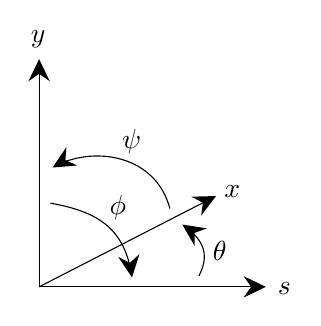
\begin{tikzpicture}[x=0.75pt,y=0.75pt,yscale=-1,xscale=1]
		%uncomment if require: \path (0,232); %set diagram left start at 0, and has height of 232

		%Straight Lines [id:da20170232008889133]
		\draw    (30.75,200.25) -- (30.75,93.5) ;
		\draw [shift={(30.75,90.5)}, rotate = 90] [fill={rgb, 255:red, 0; green, 0; blue, 0 }  ][line width=0.08]  [draw opacity=0] (10.72,-5.15) -- (0,0) -- (10.72,5.15) -- (7.12,0) -- cycle    ;
		%Straight Lines [id:da7586738429193832]
		\draw    (30.75,200.25) -- (137,200.25) ;
		\draw [shift={(140,200.25)}, rotate = 180] [fill={rgb, 255:red, 0; green, 0; blue, 0 }  ][line width=0.08]  [draw opacity=0] (10.72,-5.15) -- (0,0) -- (10.72,5.15) -- (7.12,0) -- cycle    ;
		%Straight Lines [id:da8289354712219019]
		\draw    (30.75,200.25) -- (113.33,157.87) ;
		\draw [shift={(116,156.5)}, rotate = 152.83] [fill={rgb, 255:red, 0; green, 0; blue, 0 }  ][line width=0.08]  [draw opacity=0] (10.72,-5.15) -- (0,0) -- (10.72,5.15) -- (7.12,0) -- cycle    ;
		%Curve Lines [id:da8619095365842171]
		\draw    (107.75,195) .. controls (111.49,187.52) and (112.39,180.04) .. (102.07,171.95) ;
		\draw [shift={(99.75,170.25)}, rotate = 34.46] [fill={rgb, 255:red, 0; green, 0; blue, 0 }  ][line width=0.08]  [draw opacity=0] (10.72,-5.15) -- (0,0) -- (10.72,5.15) -- (7.12,0) -- cycle    ;
		%Curve Lines [id:da14562765286410684]
		\draw    (93.75,162.5) .. controls (86.83,136.71) and (58.01,132.59) .. (39.76,141.42) ;
		\draw [shift={(37.25,142.75)}, rotate = 329.74] [fill={rgb, 255:red, 0; green, 0; blue, 0 }  ][line width=0.08]  [draw opacity=0] (10.72,-5.15) -- (0,0) -- (10.72,5.15) -- (7.12,0) -- cycle    ;
		%Curve Lines [id:da5921182448586806]
		\draw    (75.01,192.73) .. controls (71.13,171.98) and (58.98,163.96) .. (36.25,159.95) ;
		\draw [shift={(75.5,195.75)}, rotate = 261.96] [fill={rgb, 255:red, 0; green, 0; blue, 0 }  ][line width=0.08]  [draw opacity=0] (10.72,-5.15) -- (0,0) -- (10.72,5.15) -- (7.12,0) -- cycle    ;

		% Text Node
		\draw (113.25,177.15) node [anchor=north west][inner sep=0.75pt]    {$\theta $};
		% Text Node
		\draw (25.5,75.65) node [anchor=north west][inner sep=0.75pt]    {$y$};
		% Text Node
		\draw (118.75,150.15) node [anchor=north west][inner sep=0.75pt]    {$x$};
		% Text Node
		\draw (144.5,197.15) node [anchor=north west][inner sep=0.75pt]    {$s$};
		% Text Node
		\draw (69.5,123.19) node [anchor=north west][inner sep=0.75pt]    {$\psi $};
		% Text Node
		\draw (63.48,154.9) node [anchor=north west][inner sep=0.75pt]    {$\phi $};
	\end{tikzpicture}
	\caption{Rotation directions in the beam coordinate system (right-handed system).}\label{fig:beam-rotations}
\end{figure}

The longitudinal momentum is
\[
	p_z = \sqrt{(1 + \delta)^2 - p_x^2 - p_y^2}.
\]

\subsection{X Rotation}

We define a scaling factor $\kappa$ arising from the coordinate system being tilted by $\phi$ about the $x$-axis:
\[
\kappa := 1 - \frac{\tan\phi \; p_y}{p_z}.
\]
The coordinate updates can be described as follows:
\[
y \leftarrow \frac{y}{\kappa \cos\phi}, \quad p_y \leftarrow p_y \cos\phi + p_z \sin\phi,
\]

\[
x \leftarrow x + \frac{y p_x \tan\phi}{\kappa p_z}, \quad \zeta \leftarrow \zeta - \frac{y \tan\phi \left(1 + \beta_0 p_\tau \right)}{\kappa p_z}.
\]

\subsection{Y Rotation}\label{sec:Yrotation}

We define a scaling factor $\kappa$ arising from the coordinate system being tilted by $\theta$ about the $y$-axis:

\[
\kappa := 1 + \frac{\tan\theta \; p_x}{p_z}.
\]

The coordinate updates can be described as follows (which can be verified with \cite{forest99}, noting the opposite convention of the angle $\theta$):

\[
x \leftarrow \frac{x}{\kappa \cos\theta},
\quad
p_x \leftarrow p_x \cos\theta - p_z \sin\theta,
\]

\[
y \leftarrow y - \frac{x\,p_y\,\tan\theta}{\kappa\,p_z},
\quad
\zeta \leftarrow \zeta + \frac{x\,\tan\theta\,(1 + \beta_0 p_\tau)}{\kappa\,p_z}.
\]

\subsection{S Rotation}

We perform a rotation in the $x$-$y$ plane by an angle $\psi$:

\[
x \leftarrow x \cos\psi + y \sin\psi,
\quad
y \leftarrow -x \sin\psi + y \cos\psi,
\]

\[
p_x \leftarrow p_x \cos\psi + p_y \sin\psi,
\quad
p_y \leftarrow -p_x \sin\psi + p_y \cos\psi.
\]


\section{Cavity time, energy errors and acceleration}

A cavity kick depends on:

\begin{equation}
\sin(2 \pi f T + \phi)
\end{equation}

where T is laboratory time.


For the most general case:

\begin{equation}
\sin(2 \pi f T + \phi) = \sin\left(2 \pi f \frac{s-\zeta}{\beta_0 c}  + \phi \right)
\end{equation}

Most codes drop the term $2 \pi f s / (\beta_0 c)$ that is

\begin{equation}
\sin(2 \pi f T + \phi) \to  \sin\left(- 2 \pi f \frac{\zeta}{\beta_0 c} + \phi\right)
\end{equation}

to make sure that a particle that is synchronous to the reference trajectory is in phase with the cavity.


\subsection{Implementing energy errors}

One can define

\begin{equation}
\begin{aligned}
s &= s_0 + n (L_0-L) + n L\\
f_{\rm rev} &= \beta_0 c / L\\
f &= h f_{\rm rev}
\end{aligned}
\end{equation}

where $s_0$ is the path length at the cavity turn at 0, $L_0$ is the design circumference, $n$ is the turn number, $h$ is the harmonic number, L is the new path length with an energy error. Indeed one could write $L=L_0(1 +\eta \delta_s)$ where $\eta$ is a constant property of the lattice.

Multiple cavities can have their own defined $L$.

Using these definitions, then


\begin{align}
\sin(2 \pi f T + \phi) =
&\sin\left(2 \pi h f_{\rm rev} \frac{s_0 + n(L_0-L) -\zeta}{\beta_0 c}  + \phi\right)\\
=&\sin\left(2 \pi h f_{\rm rev} \frac{n(L_0-L) -\zeta}{\beta_0 c}  + \phi'\right)
\end{align}


where $\phi'=\frac{2\pi h s_0}{L} + \phi$.


In MAD-X Twiss and MAD8, the longitudinal coordinate is directly $\zeta'=n(L_0-L) -\zeta$ and the term $n(L_0-L)$ is added smoothly in each thick element. This forces all the cavities to share the same $L$ or $f_{\rm rev}$.

In SixTrack or MAD-X track, one could simply define a turn-dependent phase
\begin{equation}
\phi=\phi_0 + 2 \pi h f_{\rm rev} n(L_0-L)
\end{equation}
which is very general, or alternatively add a special element that performs at each turn the following transformation:

\begin{equation}
\zeta_{\rm new}=(L_0-L) -\zeta_{\rm old}
\end{equation}

\subsection{Acceleration}

Acceleration can be achieved by renormalizing the relative variables using a new momentum reference. This has the side effect that the fields of the magnets (expressed in normalized strength) follow the energy ramp and that the cavity frequency (if expressed in terms of the harmonic number; NB we should perhaps change this in the Xtrack interface) is updated.

The re-normalization, if done once at each turn, is:

\begin{align}
p_{x,\rm new} &= p_{x,\rm old} \frac{P_{0,\rm old}}{P_{0,\rm new}} &
p_{y,\rm new} &= p_{y,\rm old} \frac{P_{0,\rm old}}{P_{0,\rm new}} \\
\delta_{\rm new}&= (\delta_{\rm old}+1) \frac{P_{0,\rm old}}{P_{0,\rm new}} -1 &
p_{\tau,\rm new} &= \frac{p_{\tau,\rm old}\, P_{0,\rm old}\,c + E_{0,\rm old} - E_{0,\rm new}}{P_{0,\rm new}c} \\
\zeta_{\rm new} &= s\beta_0 \left(\frac{1}{\beta_{0,\rm new}} -
\frac{1}{\beta_{0,\rm old}}\right) - \zeta_{\rm old} &
\tau_{\rm new} &= s\left(\frac{1}{\beta_{0,\rm new}} -  \frac{1}{\beta_{0,\rm old}}\right) - \tau_{\rm old} \\
\end{align}


\chapter{Misalignments}\label{chapter:misalignments}

\section{Definitions}\label{section:definitions}

For defining the misalignments, we use the MAD-like coordinate system, where $s$
is the axis tangent to the reference trajectory at the entrance to the element,
and $x$ and $y$ are the transverse beam coordinates.

A misalignment of an element is characterized by seven quantities, as illustrated in
Figs.~\ref{fig:misalignment_yaw}, \ref{fig:misalignment_pitch}, and \ref{fig:misalignment_roll}:
\begin{itemize}
	\item A reference point (anchor) along the reference trajectory through the unperturbed element;
	\item 6 parameters specifying the shifts and rotations of the element with respect
        to the reference frame defined at the anchor point.
\end{itemize}

In the derivation we omit $\Delta$ in the naming of shifts and drifts and we call
\begin{equation}
  f = \frac{\Delta s_\text{anchor}}{L}
\end{equation}
the relative position of the anchor along the element of length $L$.

Note that the rotation about the $y$ axis does not follow the classical right-handed approach:
a positive $\phi$ rotation is clockwise when viewed from the positive $x$ side, i.e., it goes from the $s$ to the $y$ axis, as opposed to from $y$ to $s$.

\begin{figure}
  \centering
  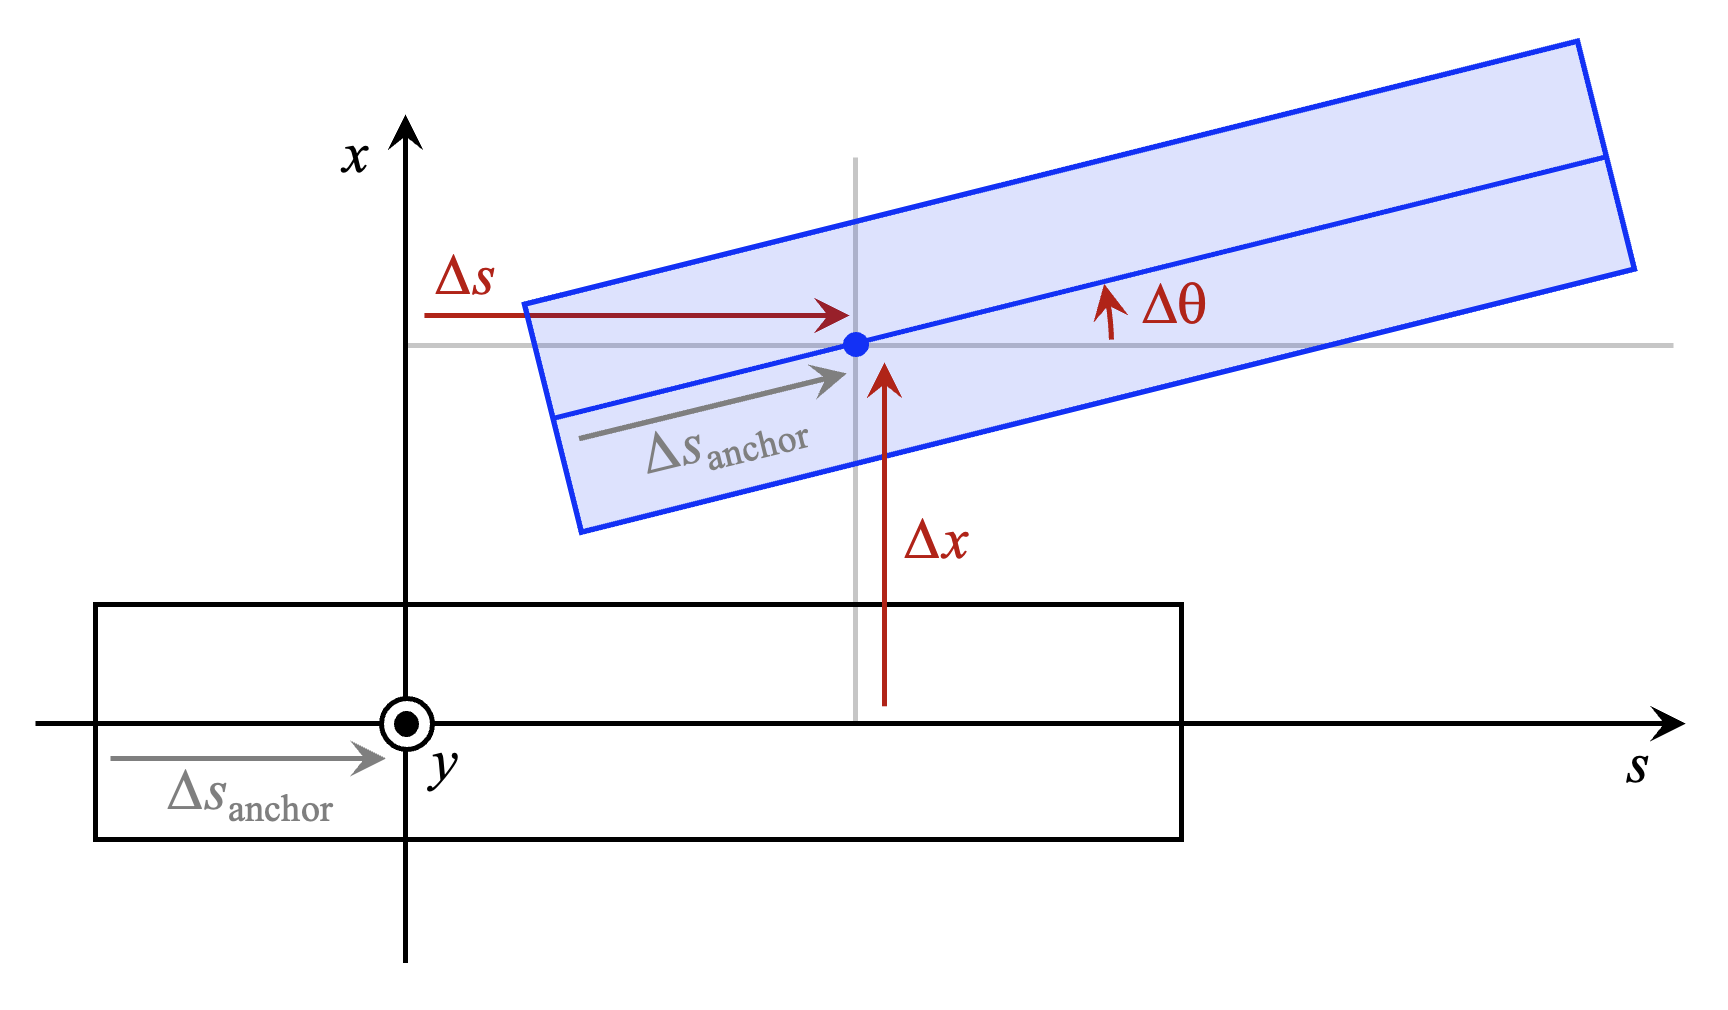
\includegraphics[width=0.8\textwidth]{figures/align_yaw.png}
  \caption{Misalignment in the s-x plane. \label{fig:misalignment_yaw}}
  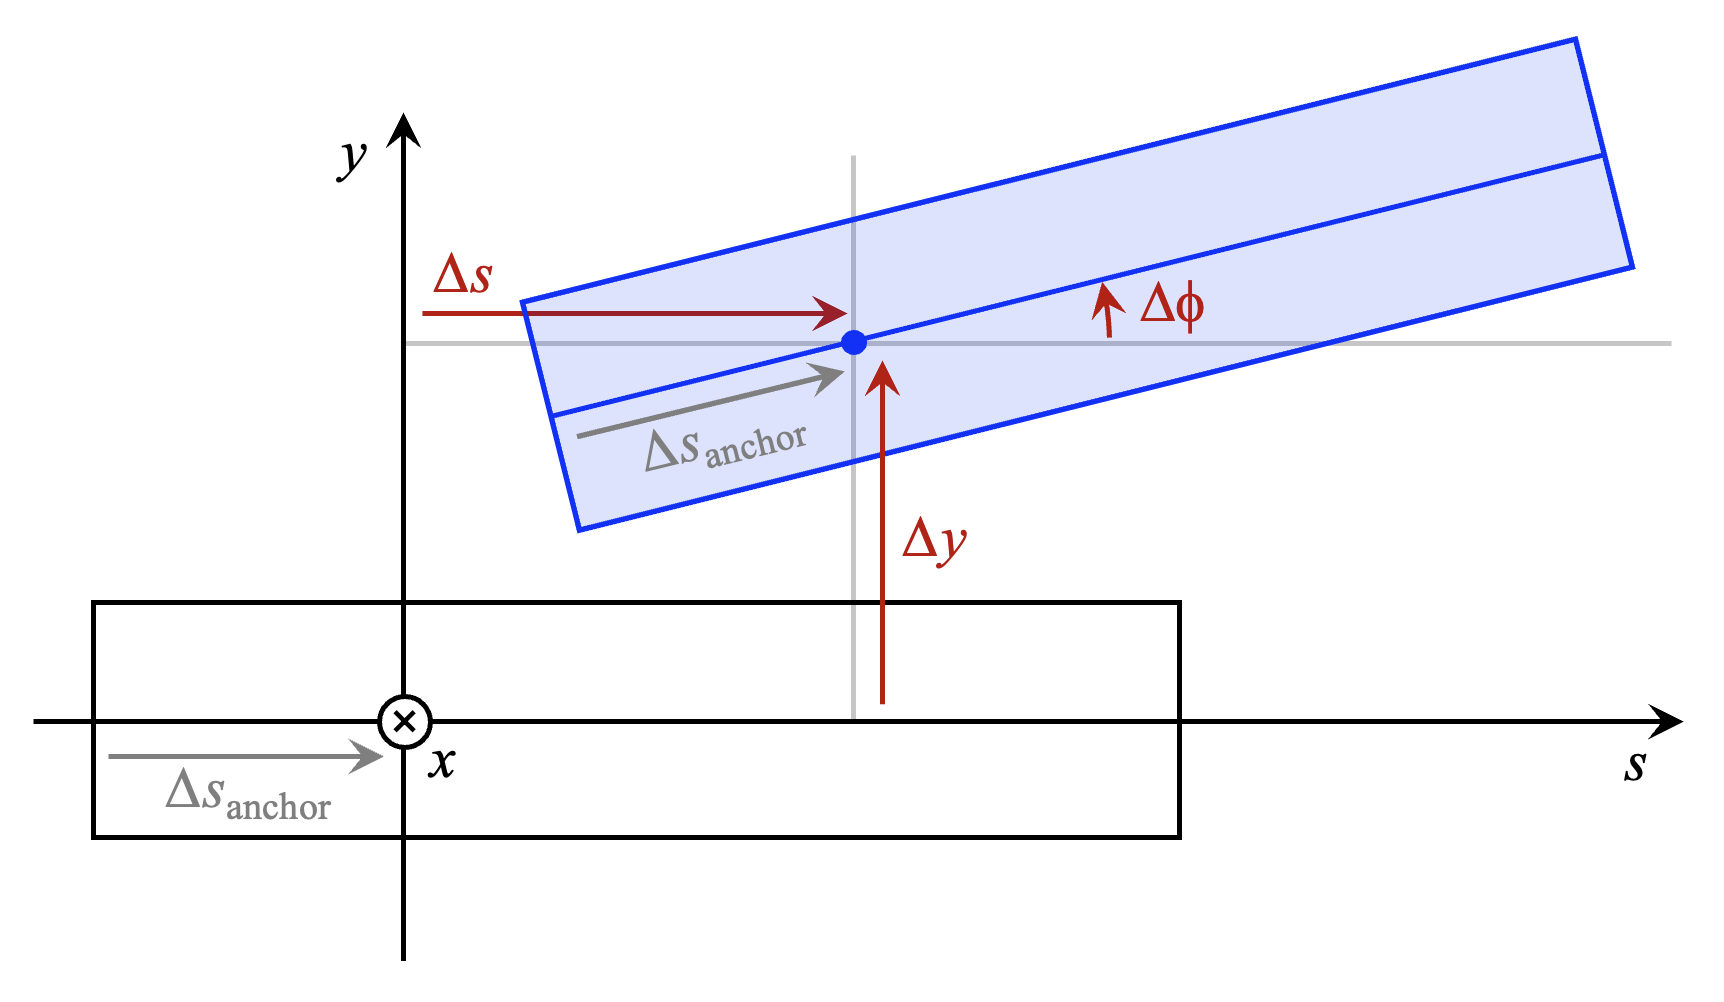
\includegraphics[width=0.8\textwidth]{figures/align_pitch.png}
  \caption{Misalignment in the s-y plane. \label{fig:misalignment_pitch}}
  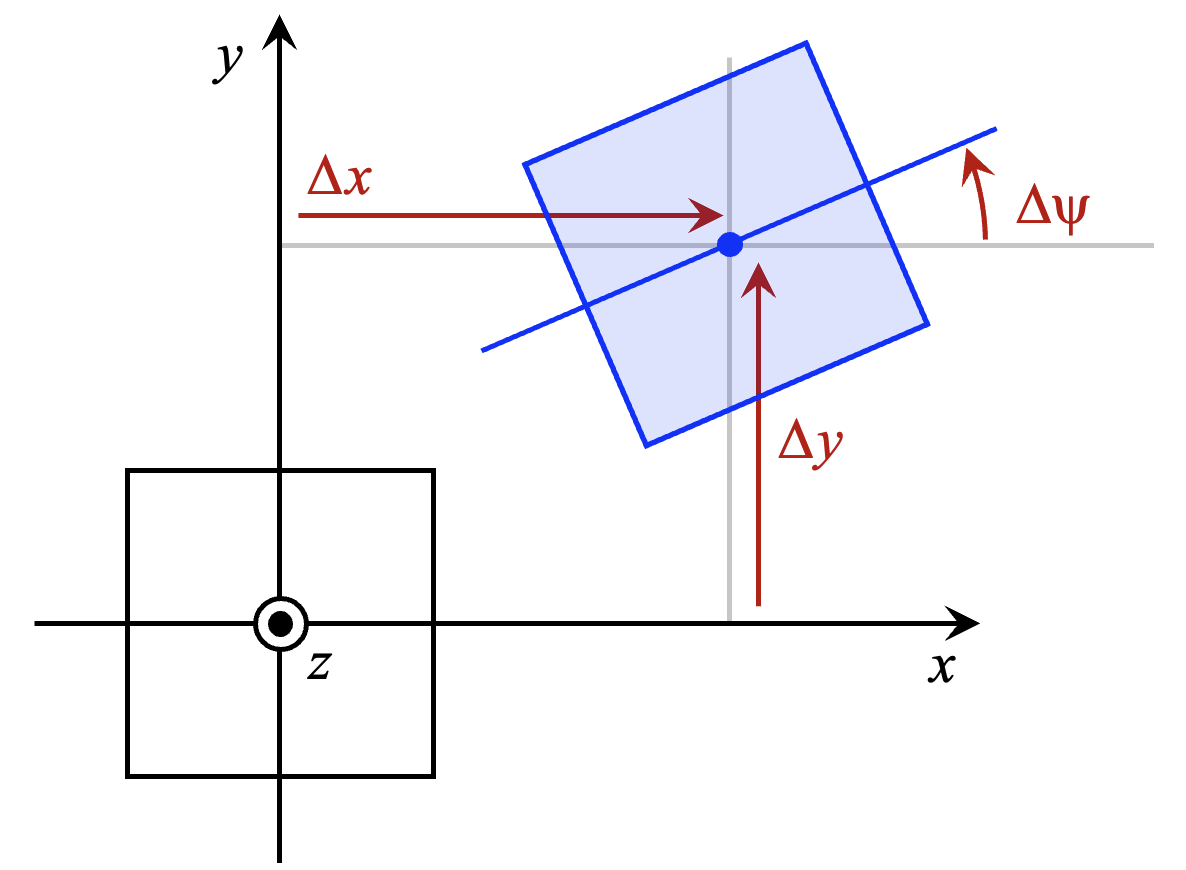
\includegraphics[width=0.5\textwidth]{figures/align_roll.png}
  \caption{Misalignment in the x-y plane. \label{fig:misalignment_roll}}
\end{figure}

For our calculations, we will represent the reference frame transformations using $4 \times 4$ augmented matrices.
We shall assume the following notation convention: each matrix $M$ consists of entries from $M_{00}$ (top left corner), through $M_{03}$ (top right corner), to $M_{33}$ (bottom right corner).
In particular, we distinguish 4 basic transformations:

\[
	\mathrm{T}(x, y, s) := \begin{bmatrix}
		1 & 0 & 0 & x \\
		0 & 1 & 0 & y \\
		0 & 0 & 1 & s \\
		0 & 0 & 0 & 1
	\end{bmatrix} \;\;\text{(translation)}
\]

\[
	\mathrm{R}_x(\phi) := \begin{bmatrix}
		1 & 0 & 0 & 0 \\
		0 & \cos(\phi) & \sin(\phi) & 0 \\
		0 & -\sin(\phi) & \cos(\phi) & 0 \\
		0 & 0 & 0 & 1
	\end{bmatrix} \;\;\text{(rotation around the $x$ axis)}
\]

\[
	\mathrm{R}_y(\theta) := \begin{bmatrix}
		\cos(\theta) & 0 & \sin(\theta) & 0 \\
		0 & 1 & 0 & 0 \\
		-\sin(\theta) & 0 & \cos(\theta) & 0 \\
		0 & 0 & 0 & 1
	\end{bmatrix} \;\;\text{(rotation around the $y$ axis)}
\]

\[
	\mathrm{R}_s(\psi) := \begin{bmatrix}
		\cos(\psi) & -\sin(\psi) & 0 & 0 \\
		\sin(\psi) & \cos(\psi) & 0 & 0 \\
		0 & 0 & 1 & 0 \\
		0 & 0 & 0 & 1
	\end{bmatrix} \;\;\text{(rotation around the $s$ axis)}
\]
We allow the notation $T_x(\Delta x)$ to mean $T(\Delta x, 0, 0)$, and so on, for $T_y(\Delta y)$ and $T_s(\Delta s)$.


\begin{figure}[H]
	\centering
	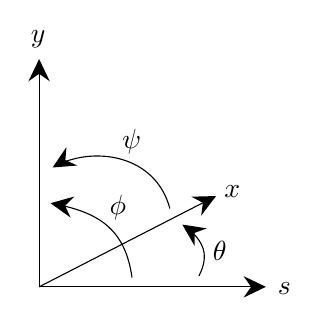
\begin{tikzpicture}[x=0.75pt,y=0.75pt,yscale=-1,xscale=1]
		%uncomment if require: \path (0,232); %set diagram left start at 0, and has height of 232

		%Straight Lines [id:da20170232008889133]
		\draw    (30.75,200.25) -- (30.75,93.5) ;
		\draw [shift={(30.75,90.5)}, rotate = 90] [fill={rgb, 255:red, 0; green, 0; blue, 0 }  ][line width=0.08]  [draw opacity=0] (10.72,-5.15) -- (0,0) -- (10.72,5.15) -- (7.12,0) -- cycle    ;
		%Straight Lines [id:da7586738429193832]
		\draw    (30.75,200.25) -- (137,200.25) ;
		\draw [shift={(140,200.25)}, rotate = 180] [fill={rgb, 255:red, 0; green, 0; blue, 0 }  ][line width=0.08]  [draw opacity=0] (10.72,-5.15) -- (0,0) -- (10.72,5.15) -- (7.12,0) -- cycle    ;
		%Straight Lines [id:da8289354712219019]
		\draw    (30.75,200.25) -- (113.33,157.87) ;
		\draw [shift={(116,156.5)}, rotate = 152.83] [fill={rgb, 255:red, 0; green, 0; blue, 0 }  ][line width=0.08]  [draw opacity=0] (10.72,-5.15) -- (0,0) -- (10.72,5.15) -- (7.12,0) -- cycle    ;
		%Curve Lines [id:da8619095365842171]
		\draw    (107.75,195) .. controls (111.49,187.52) and (112.39,180.04) .. (102.07,171.95) ;
		\draw [shift={(99.75,170.25)}, rotate = 34.46] [fill={rgb, 255:red, 0; green, 0; blue, 0 }  ][line width=0.08]  [draw opacity=0] (10.72,-5.15) -- (0,0) -- (10.72,5.15) -- (7.12,0) -- cycle    ;
		%Curve Lines [id:da14562765286410684]
		\draw    (93.75,162.5) .. controls (86.83,136.71) and (58.01,132.59) .. (39.76,141.42) ;
		\draw [shift={(37.25,142.75)}, rotate = 329.74] [fill={rgb, 255:red, 0; green, 0; blue, 0 }  ][line width=0.08]  [draw opacity=0] (10.72,-5.15) -- (0,0) -- (10.72,5.15) -- (7.12,0) -- cycle    ;
		%Curve Lines [id:da5921182448586806]
		\draw    (75.5,195.75) .. controls (72.38,173.67) and (61.01,164.86) .. (39.05,160.48) ;
		\draw [shift={(36.25,159.95)}, rotate = 10.01] [fill={rgb, 255:red, 0; green, 0; blue, 0 }  ][line width=0.08]  [draw opacity=0] (10.72,-5.15) -- (0,0) -- (10.72,5.15) -- (7.12,0) -- cycle    ;

		% Text Node
		\draw (113.25,177.15) node [anchor=north west][inner sep=0.75pt]    {$\theta $};
		% Text Node
		\draw (25.5,75.65) node [anchor=north west][inner sep=0.75pt]    {$y$};
		% Text Node
		\draw (118.75,150.15) node [anchor=north west][inner sep=0.75pt]    {$x$};
		% Text Node
		\draw (144.5,197.15) node [anchor=north west][inner sep=0.75pt]    {$s$};
		% Text Node
		\draw (69.5,123.19) node [anchor=north west][inner sep=0.75pt]    {$\psi $};
		% Text Node
		\draw (63.48,154.9) node [anchor=north west][inner sep=0.75pt]    {$\phi $};
	\end{tikzpicture}
	\caption{MAD-like coordinate system}\label{fig:mad-like-coordinates}
\end{figure}

\section{Misalignment at arbitrary $s$ without a tilt}\label{section:curved-no-roll}

We consider a potentially curved element misaligned with respect to an arbitrary position along its length.

\begin{figure}[H]
	\centering
	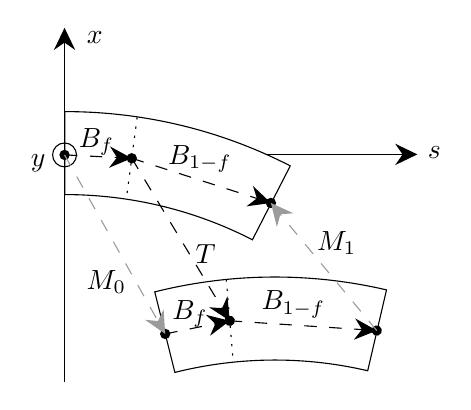
\begin{tikzpicture}[x=0.75pt,y=0.75pt,yscale=-1,xscale=1]
		%uncomment if require: \path (0,300); %set diagram left start at 0, and has height of 300

		%Straight Lines [id:da797458358196216]
		\draw    (121.25,70.82) -- (191.11,70.82) ;
		\draw [shift={(194.11,70.82)}, rotate = 180] [fill={rgb, 255:red, 0; green, 0; blue, 0 }  ][line width=0.08]  [draw opacity=0] (10.72,-5.15) -- (0,0) -- (10.72,5.15) -- (7.12,0) -- cycle    ;
		%Straight Lines [id:da5268015128426032]
		\draw    (24.11,180.32) -- (24.11,12.82) ;
		\draw [shift={(24.11,9.82)}, rotate = 90] [fill={rgb, 255:red, 0; green, 0; blue, 0 }  ][line width=0.08]  [draw opacity=0] (10.72,-5.15) -- (0,0) -- (10.72,5.15) -- (7.12,0) -- cycle    ;
		%Shape: Ellipse [id:dp6042944787247156]
		\draw   (20.02,75.11) .. controls (17.78,72.86) and (17.8,69.22) .. (20.06,66.98) .. controls (22.32,64.75) and (25.96,64.77) .. (28.19,67.02) .. controls (30.43,69.28) and (30.41,72.92) .. (28.15,75.16) .. controls (25.89,77.39) and (22.25,77.37) .. (20.02,75.11) -- cycle ;
		%Flowchart: Connector [id:dp3071692594828601]
		\draw  [draw opacity=0][fill={rgb, 255:red, 0; green, 0; blue, 0 }  ,fill opacity=1 ] (21.61,71.07) .. controls (21.61,69.69) and (22.72,68.57) .. (24.11,68.57) .. controls (25.49,68.57) and (26.61,69.69) .. (26.61,71.07) .. controls (26.61,72.45) and (25.49,73.57) .. (24.11,73.57) .. controls (22.72,73.57) and (21.61,72.45) .. (21.61,71.07) -- cycle ;

		%Shape: Block Arc [id:dp07942148731975829]
		\draw   (24.3,50.19) .. controls (24.5,50.19) and (24.69,50.19) .. (24.89,50.2) .. controls (63.78,50.3) and (100.48,59.73) .. (132.86,76.36) -- (114.62,111.95) .. controls (87.67,98.12) and (57.14,90.27) .. (24.77,90.18) .. controls (24.61,90.18) and (24.45,90.18) .. (24.29,90.18) -- cycle ;
		%Flowchart: Connector [id:dp3735648309295102]
		\draw  [draw opacity=0][fill={rgb, 255:red, 0; green, 0; blue, 0 }  ,fill opacity=1 ] (121.04,94.28) .. controls (121.01,92.9) and (122.1,91.75) .. (123.48,91.72) .. controls (124.86,91.69) and (126.01,92.78) .. (126.04,94.16) .. controls (126.07,95.54) and (124.98,96.69) .. (123.6,96.72) .. controls (122.22,96.75) and (121.07,95.66) .. (121.04,94.28) -- cycle ;
		%Straight Lines [id:da2366039478899269]
		\draw  [dash pattern={on 4.5pt off 4.5pt}]  (24.28,71.06) -- (53.48,72.52) ;
		\draw [shift={(56.48,72.67)}, rotate = 182.86] [fill={rgb, 255:red, 0; green, 0; blue, 0 }  ][line width=0.08]  [draw opacity=0] (10.72,-5.15) -- (0,0) -- (10.72,5.15) -- (7.12,0) -- cycle    ;
		%Flowchart: Connector [id:dp8051968426783745]
		\draw  [draw opacity=0][fill={rgb, 255:red, 0; green, 0; blue, 0 }  ,fill opacity=1 ] (53.98,72.73) .. controls (53.95,71.35) and (55.04,70.21) .. (56.42,70.18) .. controls (57.8,70.14) and (58.95,71.24) .. (58.98,72.62) .. controls (59.01,74) and (57.92,75.14) .. (56.54,75.17) .. controls (55.16,75.21) and (54.01,74.11) .. (53.98,72.73) -- cycle ;
		%Straight Lines [id:da5904317932248363]
		\draw  [dash pattern={on 4.5pt off 4.5pt}]  (56.48,72.67) -- (120.68,93.3) ;
		\draw [shift={(123.54,94.22)}, rotate = 197.81] [fill={rgb, 255:red, 0; green, 0; blue, 0 }  ][line width=0.08]  [draw opacity=0] (10.72,-5.15) -- (0,0) -- (10.72,5.15) -- (7.12,0) -- cycle    ;
		%Shape: Block Arc [id:dp3422197187906486]
		\draw   (67.57,137.06) .. controls (67.76,137.01) and (67.94,136.96) .. (68.13,136.92) .. controls (105.89,127.58) and (143.78,127.83) .. (179.23,136.1) -- (170.17,175.06) .. controls (140.67,168.17) and (109.15,167.97) .. (77.73,175.74) .. controls (77.57,175.77) and (77.41,175.81) .. (77.26,175.85) -- cycle ;
		%Flowchart: Connector [id:dp3058023403472935]
		\draw  [draw opacity=0][fill={rgb, 255:red, 0; green, 0; blue, 0 }  ,fill opacity=1 ] (172.11,156.36) .. controls (171.74,155.03) and (172.53,153.65) .. (173.86,153.28) .. controls (175.19,152.92) and (176.56,153.7) .. (176.93,155.03) .. controls (177.3,156.36) and (176.51,157.74) .. (175.18,158.11) .. controls (173.85,158.47) and (172.48,157.69) .. (172.11,156.36) -- cycle ;
		%Straight Lines [id:da06890321170988856]
		\draw  [dash pattern={on 4.5pt off 4.5pt}]  (72.6,157.31) -- (100.77,151.6) ;
		\draw [shift={(103.71,151)}, rotate = 168.53] [fill={rgb, 255:red, 0; green, 0; blue, 0 }  ][line width=0.08]  [draw opacity=0] (10.72,-5.15) -- (0,0) -- (10.72,5.15) -- (7.12,0) -- cycle    ;
		%Flowchart: Connector [id:dp2878241642690408]
		\draw  [draw opacity=0][fill={rgb, 255:red, 0; green, 0; blue, 0 }  ,fill opacity=1 ] (101.3,151.66) .. controls (100.93,150.33) and (101.71,148.96) .. (103.04,148.59) .. controls (104.38,148.22) and (105.75,149.01) .. (106.12,150.34) .. controls (106.48,151.67) and (105.7,153.05) .. (104.37,153.41) .. controls (103.04,153.78) and (101.66,153) .. (101.3,151.66) -- cycle ;
		%Straight Lines [id:da3521010885853867]
		\draw  [dash pattern={on 4.5pt off 4.5pt}]  (103.71,151) -- (171.53,155.5) ;
		\draw [shift={(174.52,155.69)}, rotate = 183.79] [fill={rgb, 255:red, 0; green, 0; blue, 0 }  ][line width=0.08]  [draw opacity=0] (10.72,-5.15) -- (0,0) -- (10.72,5.15) -- (7.12,0) -- cycle    ;
		%Flowchart: Connector [id:dp35613516370993914]
		\draw  [draw opacity=0][fill={rgb, 255:red, 0; green, 0; blue, 0 }  ,fill opacity=1 ] (70.1,157.37) .. controls (70.07,155.99) and (71.17,154.84) .. (72.55,154.81) .. controls (73.93,154.78) and (75.07,155.87) .. (75.1,157.25) .. controls (75.14,158.63) and (74.04,159.78) .. (72.66,159.81) .. controls (71.28,159.84) and (70.14,158.75) .. (70.1,157.37) -- cycle ;
		%Straight Lines [id:da881388803539509]
		\draw  [dash pattern={on 4.5pt off 4.5pt}]  (56.48,72.67) -- (102.16,148.43) ;
		\draw [shift={(103.71,151)}, rotate = 238.91] [fill={rgb, 255:red, 0; green, 0; blue, 0 }  ][line width=0.08]  [draw opacity=0] (10.72,-5.15) -- (0,0) -- (10.72,5.15) -- (7.12,0) -- cycle    ;
		%Straight Lines [id:da07326003199202691]
		\draw [color={rgb, 255:red, 155; green, 155; blue, 155 }  ,draw opacity=1 ] [dash pattern={on 4.5pt off 4.5pt}]  (24.11,71.07) -- (71.13,154.7) ;
		\draw [shift={(72.6,157.31)}, rotate = 240.65] [fill={rgb, 255:red, 155; green, 155; blue, 155 }  ,fill opacity=1 ][line width=0.08]  [draw opacity=0] (10.72,-5.15) -- (0,0) -- (10.72,5.15) -- (7.12,0) -- cycle    ;
		%Straight Lines [id:da5449253722191645]
		\draw [color={rgb, 255:red, 155; green, 155; blue, 155 }  ,draw opacity=1 ] [dash pattern={on 4.5pt off 4.5pt}]  (174.52,155.69) -- (125.45,96.53) ;
		\draw [shift={(123.54,94.22)}, rotate = 50.33] [fill={rgb, 255:red, 155; green, 155; blue, 155 }  ,fill opacity=1 ][line width=0.08]  [draw opacity=0] (10.72,-5.15) -- (0,0) -- (10.72,5.15) -- (7.12,0) -- cycle    ;
		%Straight Lines [id:da0006877697562143181]
		\draw  [dash pattern={on 0.84pt off 2.51pt}]  (59.1,52.92) -- (53.85,92.42) ;
		%Straight Lines [id:da06332771626503675]
		\draw  [dash pattern={on 0.84pt off 2.51pt}]  (102.03,131.04) -- (105.38,170.96) ;

		% Text Node
		\draw (33.61,10.47) node [anchor=north west][inner sep=0.75pt]    {$x$};
		% Text Node
		\draw (197.86,65.97) node [anchor=north west][inner sep=0.75pt]    {$s$};
		% Text Node
		\draw (6.61,69.72) node [anchor=north west][inner sep=0.75pt]    {$y$};
		% Text Node
		\draw (29.75,57.15) node [anchor=north west][inner sep=0.75pt]    {$B_{f}$};
		% Text Node
		\draw (72.75,65.4) node [anchor=north west][inner sep=0.75pt]    {$B_{1-f}$};
		% Text Node
		\draw (74.75,140.15) node [anchor=north west][inner sep=0.75pt]    {$B_{f}$};
		% Text Node
		\draw (117.75,135.4) node [anchor=north west][inner sep=0.75pt]    {$B_{1-f}$};
		% Text Node
		\draw (86,112.9) node [anchor=north west][inner sep=0.75pt]    {$T$};
		% Text Node
		\draw (33.5,125.4) node [anchor=north west][inner sep=0.75pt]    {$M_{0}$};
		% Text Node
		\draw (144.5,106.65) node [anchor=north west][inner sep=0.75pt]    {$M_{1}$};
	\end{tikzpicture}
	\caption{Transformations for a curved element misaligned at an arbitrary $s$.}
\end{figure}

Assuming a curved element of length $L$ that bends the reference frame by $\alpha$ (and therefore a radius of curvature $\rho = L / \alpha$), we can represent $B$ as a combination of a translation and a rotation, $B := T(\Delta x, 0, \Delta s) R_y(-\alpha)$, where
\begin{equation}\label{eq:curved-frame-change}
	\begin{aligned}
		\Delta x &= \rho (\cos(\alpha) - 1) = - L \mathrm{sinc}(\alpha / 2) \sin(\alpha / 2), \\
		\Delta s &= \rho \sin(\alpha) = L \mathrm{sinc}(\alpha).
	\end{aligned}
\end{equation}
Note that the second formulations of $\Delta x$ and $\Delta s$ let us avoid division by zero if $\alpha = 0$, catering also to the case of a straight element for a truly general case.

Let us say that our element is misaligned at position $\Delta L$ along its length $L$.
Then we can decompose our reference-frame-bending transformation $B$ into parts $B_f$ and $B_{1-f}$ so that $B = B_f B_{1-f}$.
The respective bending angles of the two parts are simply $f \alpha$ and $(1 - f) \alpha$, where $f := \Delta L/L = \Delta L / (\rho \alpha)$ and $\rho$ is the radius of curvature.
Knowing these parameters, it is trivial to construct $B_f$ and $B_{1 - f}$ analogously to $B$, as shown in Eq.~\ref{eq:curved-frame-change}.

Then, we compute the following transformation, which will take us from the normal to the misaligned element entry frame:
\[
	M_0 = B_f T B_f^{-1},
\]
whereas for returning to the normal frame from the exit
\[
	\begin{aligned}
		B_f T B_{1 - f} M_1 &= B = B_f B_{1-f}, \\
		M_1 &= (T B_{1 - f})^{-1} B_{1-f} = B_{1 - f}^{-1} T^{-1} B_{1-f}.
	\end{aligned}
\]

When evaluated, the matrix for the curved element in the general case is
\[
	B_f := \begin{bmatrix}
		\cos\left(\alpha f\right) & 0 & -\sin\left(\alpha f\right) & \rho (\cos\left(\alpha f\right) - 1) \\
		0 & 1 & 0 & 0 \\
		\sin\left(\alpha f\right) & 0 & \cos\left(\alpha f\right) & \rho \sin(\alpha f) \\
		0 & 0 & 0 & 1
	\end{bmatrix},
\]
and so
\[
	B_f^{-1} := \begin{bmatrix}
			\cos\left(\alpha f\right) & 0 & \sin\left(\alpha f\right) & \rho (\cos\left(\alpha f\right) - 1) \\
		0 & 1 & 0 & 0 \\
		-\sin\left(\alpha f\right) & 0 & \cos\left(\alpha f\right) & - \rho \sin(\alpha f) \\
		0 & 0 & 0 & 1
		\end{bmatrix}.
\]
Note that $B_{f,03} = (B_f^{-1})_{03} = -L f \mathrm{sinc}(\alpha f / 2) \sin(\alpha f / 2)$ and $B_{f,23} = -(B_f^{-1})_{23} = L f \mathrm{sinc}(\alpha f)$.

Meanwhile, the misalignment matrix is (let $s_\phi := \sin(\phi)$, $c_\psi := \cos(\psi)$, etc., for space-saving reasons)
\[
	T = \begin{bmatrix}
		-s_\phi s_\psi s_\theta + c_\psi c_\theta & -c_\psi s_\phi s_\theta - c_\theta s_\psi & c_\phi s_\theta & x \\
		c_\phi s_\psi & c_\phi c_\psi & s_\phi & y \\
		-c_\theta s_\phi s_\psi - c_\psi s_\theta & -c_\psi c_\theta s_\phi + s_\psi s_\theta & c_\phi c_\theta & s \\
		0 & 0 & 0 & 1
	\end{bmatrix}
\]
and its inverse, since $T$ is a rigid affine transformation, can be computed with
\[
	T^{-1} = \begin{bmatrix}
			R^T & -R^T t \\
			0 & 1
		\end{bmatrix}, \text{ given } \begin{bmatrix}
			R & t \\
			0 & 1
		\end{bmatrix} := T.
\]
%which expands into the matrix
%\[
%	\begin{bmatrix}
%		-s_\phi s_\psi s_\theta + c_\psi c_\theta & c_\phi s_\psi & -c_\theta s_\phi s_\psi - c_\psi s_\theta & (s_\phi s_\psi s - c_\psi x) c_\theta + (s_\phi s_\psi x + c_\psi s) s_\theta - c_\phi s_\psi y \\
%		-c_\psi s_\phi s_\theta - c_\theta s_\psi & c_\phi c_\psi & -c_\psi c_\theta s_\phi + s_\psi s_\theta & (c_\psi s_\phi s + s_\psi x) c_\theta + (c_\psi s_\phi x - s_\psi s) s_\theta - c_\phi c_\psi y \\
%		c_\phi s_\theta & s_\phi & c_\phi c_\theta & -c_\phi c_\theta s - c_\phi s_\theta x - s_\phi y \\
%		0 & 0 & 0 & 1
%	\end{bmatrix}.
%\]

For the conversion from $M_0$ and $M_1$ to the basic tracking transformations, we can use the decomposition, $M_0 = T(x_0, y_0, s_0) R_y(\theta_0) R_x(\phi_0) R_s(\psi_0)$, for which the parameters are as follows
\[
	\begin{aligned}
		\theta_0 &= \arctan_2(M_{0,02}, M_{0,22}), \\
		\phi_0 &= \arctan_2(M_{0,12}, \sqrt{M_{0,10}^2 + M_{0,11}^2}), \\
		\psi_0 &= \arctan_2(M_{0,10}, M_{0,11}), \\
		x_0 &= M_{0,03}, \\
		y_0 &= M_{0,13}, \\
		s_0 &= M_{0,23},
	\end{aligned}
\]
and for the exit, $M_1 = T(x_1, y_1, s_1) R_y(\theta_1) R_x(\phi_1) R_s(\psi_1)$,
\[
	\begin{aligned}
		\theta_1 &= \arctan_2(M_{1,02}, M_{1,22}), \\
		\phi_1 &= \arctan_2(M_{1,12}, \sqrt{M_{1,10}^2 + M_{1,11}^2}), \\
		\psi_1 &= \arctan_2(M_{1,10}, M_{1,11}), \\
		x_1 &= M_{1,03}, \\
		y_1 &= M_{1,13}, \\
		s_1 &= M_{1,23}.
	\end{aligned}
\]
Note that many decompositions are possible, and their order can lead to more or less clean closed formulae for the parameters; in this case, however, we do not expect any `nice' closed-form solutions (as opposed to the case of the subsequent section!).
The above decomposition corresponds to the following tracking sequence:
\begin{itemize}
	\item ($M_0$:) XYShift($x_0$, $y_0$), SShift($s_0$), YRot($\theta_0$), XRot($\phi_0$), SRot($\psi_0$),
	\item ($B$:) Element($L$, $\alpha$),
	\item ($M_1$:) XYShift($x_1$, $y_1$), SShift($s_1$), YRot($\theta_1$), XRot($\phi_1$), SRot($\psi_1$).
\end{itemize}


\section{Misalignment at arbitrary $s$ (the straight case)}\label{section:straight}

Analogously to the previous section, we split $D$ into $D_f D_{1-f}$:
\begin{figure}[H]
	\centering
	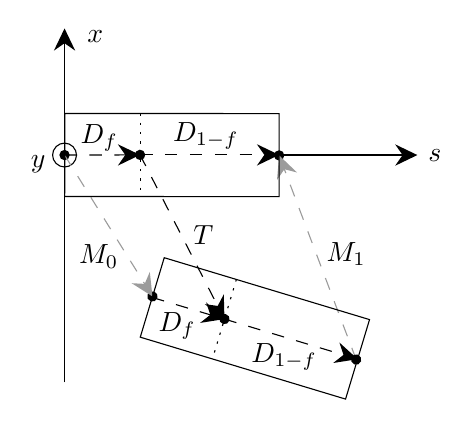
\begin{tikzpicture}[x=0.75pt,y=0.75pt,yscale=-1,xscale=1]
		%uncomment if require: \path (0,300); %set diagram left start at 0, and has height of 300

		%Straight Lines [id:da35507818785418455]
		\draw    (127.5,70.82) -- (191.11,70.82) ;
		\draw [shift={(194.11,70.82)}, rotate = 180] [fill={rgb, 255:red, 0; green, 0; blue, 0 }  ][line width=0.08]  [draw opacity=0] (10.72,-5.15) -- (0,0) -- (10.72,5.15) -- (7.12,0) -- cycle    ;
		%Straight Lines [id:da8526813980418886]
		\draw    (24.11,180.32) -- (24.11,12.82) ;
		\draw [shift={(24.11,9.82)}, rotate = 90] [fill={rgb, 255:red, 0; green, 0; blue, 0 }  ][line width=0.08]  [draw opacity=0] (10.72,-5.15) -- (0,0) -- (10.72,5.15) -- (7.12,0) -- cycle    ;
		%Flowchart: Connector [id:dp5359668052415314]
		\draw  [draw opacity=0][fill={rgb, 255:red, 0; green, 0; blue, 0 }  ,fill opacity=1 ] (125,71) .. controls (125,69.62) and (126.12,68.5) .. (127.5,68.5) .. controls (128.88,68.5) and (130,69.62) .. (130,71) .. controls (130,72.38) and (128.88,73.5) .. (127.5,73.5) .. controls (126.12,73.5) and (125,72.38) .. (125,71) -- cycle ;
		%Straight Lines [id:da6177744279918915]
		\draw [color={rgb, 255:red, 155; green, 155; blue, 155 }  ,draw opacity=1 ] [dash pattern={on 4.5pt off 4.5pt}]  (164.61,169.34) -- (128.56,73.81) ;
		\draw [shift={(127.5,71)}, rotate = 69.32] [fill={rgb, 255:red, 155; green, 155; blue, 155 }  ,fill opacity=1 ][line width=0.08]  [draw opacity=0] (10.72,-5.15) -- (0,0) -- (10.72,5.15) -- (7.12,0) -- cycle    ;
		%Flowchart: Connector [id:dp7969702218848098]
		\draw  [draw opacity=0][fill={rgb, 255:red, 0; green, 0; blue, 0 }  ,fill opacity=1 ] (64.14,138.06) .. controls (64.63,136.77) and (66.07,136.12) .. (67.36,136.62) .. controls (68.65,137.11) and (69.3,138.55) .. (68.81,139.84) .. controls (68.32,141.13) and (66.87,141.78) .. (65.58,141.29) .. controls (64.29,140.8) and (63.65,139.35) .. (64.14,138.06) -- cycle ;
		%Flowchart: Connector [id:dp09475937969231463]
		\draw  [draw opacity=0][fill={rgb, 255:red, 0; green, 0; blue, 0 }  ,fill opacity=1 ] (162.27,168.45) .. controls (162.77,167.16) and (164.21,166.51) .. (165.5,167) .. controls (166.79,167.49) and (167.44,168.94) .. (166.95,170.23) .. controls (166.45,171.52) and (165.01,172.16) .. (163.72,171.67) .. controls (162.43,171.18) and (161.78,169.74) .. (162.27,168.45) -- cycle ;
		%Shape: Ellipse [id:dp5244406786344289]
		\draw   (20.02,74.86) .. controls (17.78,72.61) and (17.8,68.97) .. (20.06,66.73) .. controls (22.32,64.5) and (25.96,64.52) .. (28.19,66.77) .. controls (30.43,69.03) and (30.41,72.67) .. (28.15,74.91) .. controls (25.89,77.14) and (22.25,77.12) .. (20.02,74.86) -- cycle ;
		%Flowchart: Connector [id:dp7900569932281408]
		\draw  [draw opacity=0][fill={rgb, 255:red, 0; green, 0; blue, 0 }  ,fill opacity=1 ] (21.61,70.82) .. controls (21.61,69.44) and (22.72,68.32) .. (24.11,68.32) .. controls (25.49,68.32) and (26.61,69.44) .. (26.61,70.82) .. controls (26.61,72.2) and (25.49,73.32) .. (24.11,73.32) .. controls (22.72,73.32) and (21.61,72.2) .. (21.61,70.82) -- cycle ;

		%Straight Lines [id:da20442801210117567]
		\draw [color={rgb, 255:red, 155; green, 155; blue, 155 }  ,draw opacity=1 ] [dash pattern={on 4.5pt off 4.5pt}]  (24.11,70.82) -- (64.89,136.4) ;
		\draw [shift={(66.47,138.95)}, rotate = 238.12] [fill={rgb, 255:red, 155; green, 155; blue, 155 }  ,fill opacity=1 ][line width=0.08]  [draw opacity=0] (10.72,-5.15) -- (0,0) -- (10.72,5.15) -- (7.12,0) -- cycle    ;
		%Straight Lines [id:da774139029064869]
		\draw  [dash pattern={on 4.5pt off 4.5pt}]  (24.11,70.82) -- (57.5,70.76) ;
		\draw [shift={(60.5,70.75)}, rotate = 179.89] [fill={rgb, 255:red, 0; green, 0; blue, 0 }  ][line width=0.08]  [draw opacity=0] (10.72,-5.15) -- (0,0) -- (10.72,5.15) -- (7.12,0) -- cycle    ;
		%Flowchart: Connector [id:dp1702286240852332]
		\draw  [draw opacity=0][fill={rgb, 255:red, 0; green, 0; blue, 0 }  ,fill opacity=1 ] (58.01,70.93) .. controls (57.91,69.55) and (58.94,68.36) .. (60.32,68.26) .. controls (61.7,68.16) and (62.89,69.19) .. (62.99,70.57) .. controls (63.09,71.95) and (62.06,73.14) .. (60.68,73.24) .. controls (59.3,73.34) and (58.11,72.31) .. (58.01,70.93) -- cycle ;
		%Straight Lines [id:da6390869763810431]
		\draw  [dash pattern={on 4.5pt off 4.5pt}]  (60.5,70.75) -- (124.5,70.75) ;
		\draw [shift={(127.5,70.75)}, rotate = 180] [fill={rgb, 255:red, 0; green, 0; blue, 0 }  ][line width=0.08]  [draw opacity=0] (10.72,-5.15) -- (0,0) -- (10.72,5.15) -- (7.12,0) -- cycle    ;
		%Shape: Rectangle [id:dp5029720108971986]
		\draw   (24.19,50.8) -- (127.5,50.84) -- (127.49,90.84) -- (24.18,90.8) -- cycle ;
		%Straight Lines [id:da5919731693823477]
		\draw  [dash pattern={on 0.84pt off 2.51pt}]  (60.5,50.75) -- (60.5,90.75) ;
		%Straight Lines [id:da7746066807011568]
		\draw  [dash pattern={on 4.5pt off 4.5pt}]  (66.29,139.41) -- (98.28,148.98) ;
		\draw [shift={(101.15,149.84)}, rotate = 196.65] [fill={rgb, 255:red, 0; green, 0; blue, 0 }  ][line width=0.08]  [draw opacity=0] (10.72,-5.15) -- (0,0) -- (10.72,5.15) -- (7.12,0) -- cycle    ;
		%Flowchart: Connector [id:dp7156618154401919]
		\draw  [draw opacity=0][fill={rgb, 255:red, 0; green, 0; blue, 0 }  ,fill opacity=1 ] (98.71,149.3) .. controls (99.02,147.95) and (100.35,147.1) .. (101.7,147.4) .. controls (103.05,147.7) and (103.9,149.04) .. (103.59,150.39) .. controls (103.29,151.74) and (101.96,152.58) .. (100.61,152.28) .. controls (99.26,151.98) and (98.41,150.65) .. (98.71,149.3) -- cycle ;
		%Straight Lines [id:da69262585053882]
		\draw  [dash pattern={on 4.5pt off 4.5pt}]  (101.15,149.84) -- (162.44,168.3) ;
		\draw [shift={(165.31,169.16)}, rotate = 196.76] [fill={rgb, 255:red, 0; green, 0; blue, 0 }  ][line width=0.08]  [draw opacity=0] (10.72,-5.15) -- (0,0) -- (10.72,5.15) -- (7.12,0) -- cycle    ;
		%Shape: Rectangle [id:dp06216288058859021]
		\draw   (72.14,120.28) -- (171.05,150.1) -- (159.5,188.4) -- (60.59,158.57) -- cycle ;
		%Straight Lines [id:da15643091065704995]
		\draw  [dash pattern={on 0.84pt off 2.51pt}]  (106.92,130.69) -- (95.39,168.99) ;
		%Straight Lines [id:da3239479052474509]
		\draw  [dash pattern={on 4.5pt off 4.5pt}]  (60.5,70.75) -- (99.78,147.18) ;
		\draw [shift={(101.15,149.84)}, rotate = 242.8] [fill={rgb, 255:red, 0; green, 0; blue, 0 }  ][line width=0.08]  [draw opacity=0] (10.72,-5.15) -- (0,0) -- (10.72,5.15) -- (7.12,0) -- cycle    ;

		% Text Node
		\draw (33.86,9.72) node [anchor=north west][inner sep=0.75pt]    {$x$};
		% Text Node
		\draw (198.11,66.72) node [anchor=north west][inner sep=0.75pt]    {$s$};
		% Text Node
		\draw (29.86,112.89) node [anchor=north west][inner sep=0.75pt]    {$M_{0}$};
		% Text Node
		\draw (149.11,111.72) node [anchor=north west][inner sep=0.75pt]    {$M_{1}$};
		% Text Node
		\draw (6.61,69.72) node [anchor=north west][inner sep=0.75pt]    {$y$};
		% Text Node
		\draw (84.86,103.47) node [anchor=north west][inner sep=0.75pt]    {$T$};
		% Text Node
		\draw (30.61,54.72) node [anchor=north west][inner sep=0.75pt]    {$D_{f}$};
		% Text Node
		\draw (68.11,145.22) node [anchor=north west][inner sep=0.75pt]    {$D_{f}$};
		% Text Node
		\draw (75.11,53.97) node [anchor=north west][inner sep=0.75pt]    {$D_{1-f}$};
		% Text Node
		\draw (112.86,160.22) node [anchor=north west][inner sep=0.75pt]    {$D_{1-f}$};
	\end{tikzpicture}
	\caption{A straight element misaligned at an arbitrary location.}
\end{figure}

We simply have that $D_f := T(0, 0, fL)$ and $D_{1-f} := T(0, 0, (1-f)L)$.
To get to the misaligned entry frame we have
\[
	M_0 := D_f T D_f^{-1} = T_s(fL) \; T \; T_s(-fL),
\]
whereas for returning to the normal frame from the exit
\[
	\begin{aligned}
		M_1 := D_{1-f}^{-1} T^{-1} D_{1-f} = T_s((f-1)L) \; T^{-1} \; T_s((1-f)L).
	\end{aligned}
\]

It is intuitively obvious that, due to the lack of curvature, the entry and exit transformations should be possible to simplify.
Specifically, we would want $M_0$ to involve some translation followed by rotations $R_y(\theta) R_x(\phi) R_s(\psi)$, and $M_1$, since it `undoes' the effect of $M_0$, to involve rotations $R_s(-\psi) R_x(-\phi) R_y(-\theta)$ followed by some other translation.

First we decompose the entry matrix $M_0 = T(x_0, y_0, s_0) R_y(\theta_0) R_x(\phi_0) R_s(\psi_0)$, i.e.~with the same method as in the previous section.
After some algebra we observe that the angles and shifts indeed simplify:
\[
	\begin{aligned}
		\theta_0 &= \arctan_2(M_{0,02}, M_{0,22}) = \theta, \\
		\phi_0 &= \arctan_2(M_{0,12}, \sqrt{M_{0,10}^2 + M_{0,11}^2}) = \phi, \\
		\psi_0 &= \arctan_2(M_{0,10}, M_{0,11}) = \psi, \\
		x_0 &= T_{0,03} = x - L f \cos(\phi)\sin(\theta), \\
		y_0 &= T_{0,13} = y - L f \sin(\phi), \\
		s_0 &= T_{0,23} = s - L f (\cos(\phi)\cos(\theta) - 1).
	\end{aligned}
\]

Let us now decompose the matrix $M_1$ into $R_s(\psi_1) R_x(\phi_1) R_y(\theta_1) T(x_1, y_1, s_1)$.
To this end, let us write separately as $M_{rot}$ and $M_{tr}$ the rotation and translation part of the above decomposition, i.e.~let $M_{rot} = R_s(\psi_1) R_x(\phi_1) R_y(\theta_1)$ and let $M_{tr} := T(x_1, y_1, s_1)$.
In such a decomposition, the rotation part of $M_{rot}$ is the same as that of $M_1$, and so we can simply extract it from there.
Afterwards, knowing $M_{rot}$ we can compute $M_{tr} = M_{rot}^{-1} M_1$ to get the shifts.
We indeed observe the angles and shifts simplifying:
\[
	\begin{aligned}
		\theta_1 &= -\arctan_2(M_{1,20}, M_{1,22}) = -\theta, \\
		\phi_1 &= -\arctan_2(M_{1,21}, \sqrt{M_{1,01}^2 + M_{1,11}^2}) = -\phi, \\
		\psi_1 &= \arctan_2(M_{1,01}, M_{1,11}) = -\psi, \\
		x_1 &= M_{tr,03} = (f - 1) L \cos(\phi) \sin(\theta) - x, \\
		y_1 &= M_{tr,13} = (f - 1) L \sin(\phi) - y, \\
		s_1 &= M_{tr,23} = (f - 1) L (\cos(\phi) \cos(\theta) - 1) - s.
	\end{aligned}
\]
This way, our tracking procedure can be significantly less computationally expensive, compared to that of the preceding section, as no matrix operations are required:
	\begin{itemize}
	\item XYShift($x - L f \cos(\phi)\sin(\theta)$, $y - L f \sin(\phi)$)
	\item SShift($s - L f (1 - \cos(\phi)\cos(\theta))$)
	\item YRot($\theta$), XRot($\phi$), SRot($\psi$),
	\item Element($L$),
	\item SRot($-\psi$), XRot($-\phi$), YRot($-\theta$),
	\item SShift($(f - 1) L (\cos(\phi) \cos(\theta) - 1) - s$),
	\item XYShift($(f - 1) L \cos(\phi) \sin(\theta) - x$, $(f - 1) L \sin(\phi) - y$).
\end{itemize}


\section{Misalignment at arbitrary $s$ with a tilt}

We consider a tilted curved element misaligned with respect to an arbitrary position along its length.

\begin{figure}[H]
	\centering
	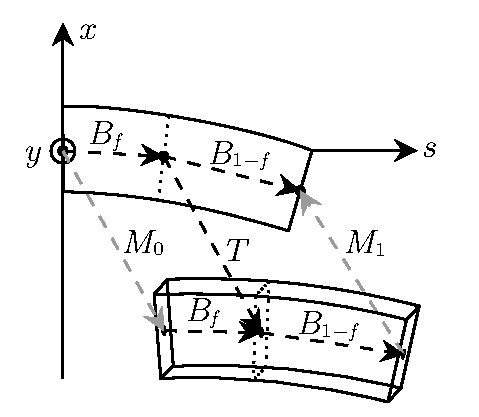
\includegraphics[scale=0.75]{figures/bend-roll.pdf}
	\caption{A tilted curved element misaligned at an arbitrary location.}
	\label{fig:bend-roll}
\end{figure}

Compared with the earlier discussion of misaligned curved elements (see Section~\ref{section:curved-no-roll}), when considering a tilted element, we need to include the tilting in our transformation $B$ (which, as before, is decomposed as $B_f B_{1-f}$ in Figure~\ref{fig:bend-roll}).

In order to include this effect we need to realize that in the previous case the curvature of the reference frame was only applied in the $s{-}x$ plane, whereas in the case of Figure~\ref{fig:bend-roll}, it will be applied in the plane obtained by tilting $s{-}x$ by some angle $\kappa$.

Therefore, taking $B_{sx}$ as the earlier transformation, i.e.,
\[
	B_{sx} := \begin{bmatrix}
		\cos\left(\alpha\right) & 0 & -\sin\left(\alpha\right) & \rho (\cos\left(\alpha\right) - 1) \\
		0 & 1 & 0 & 0 \\
		\sin\left(\alpha\right) & 0 & \cos\left(\alpha\right) & \rho \sin(\alpha) \\
		0 & 0 & 0 & 1
	\end{bmatrix},
\]
and taking $s_\alpha = \sin(\alpha)$, $c_\alpha = \cos(\alpha)$, etc.~for space-saving reasons, we can express $B$ as $R_s(\kappa) \; B_{sx} \; R_s(-\kappa)$, which evaluates to
\[
	B := \begin{bmatrix}
		{\left(c_\alpha - 1\right)} c_\kappa^{2} + 1 & {\left(c_\alpha - 1\right)} c_\kappa s_\kappa & -c_\kappa s_\alpha & \rho {\left(c_\alpha - 1\right)} c_\kappa \\
		{\left(c_\alpha - 1\right)} c_\kappa s_\kappa & {\left(c_\alpha - 1\right)} s_\kappa^{2} + 1 & -s_\alpha s_\kappa & \rho {\left(c_\alpha - 1\right)} s_\kappa \\
		c_\kappa s_\alpha & s_\alpha s_\kappa & c_\alpha & \rho s_\alpha \\
		0 & 0 & 0 & 1
	\end{bmatrix}.
\]
We can obtain the matrices $B_f$ and $B_{1-f}$ by substituting $f \alpha$ and $(1 - f) \alpha$ for $\alpha$ in the above.
To obtain the tracking procedure in this case it suffices to follow the steps of Section~\ref{section:curved-no-roll}, substituting the new matrices.


\section{Misalignment at arbitrary $s$ with a tilt (straight case)}\label{section:straight-roll}

We can generalize the matrix of the above section to a straight case by recalling that $\rho(\cos(\alpha) - 1) = -L \mathrm{sinc}(\alpha / 2) \sin(\alpha / 2)$ and $\rho \sin(\alpha) = L \mathrm{sinc}(\alpha)$.
Then, we can see that when $\alpha = 0$, the matrix $B$ of the preceding section simplifies to
\[
	B \rvert_{\alpha=0} = \begin{bmatrix}
		1 & 0 & 0 & 0 \\
		0 & 1 & 0 & 0 \\
		0 & 0 & 1 & L \\
		0 & 0 & 0 & 1
	\end{bmatrix} = T_s(L) = D.
\]
This means that the effect of the roll is disregarded in the calculation of the reference frame change for the purposes of a misalignment, and, therefore, that we can apply the exact procedure outlined in Section~\ref{section:straight} also for tilted elements.
This makes intuitive sense, as, in our setup, the tilt indeed only affects the direction of curvature of the element: if the element is straight, there is no work to be done for the misalignment, and the element map alone fully describes the effect of the tilt on the particles.


\section{S Shift -- $\zeta$ correction}

In the tracking procedures shown in the preceding sections, we use the tracking map we refer to as an SShift, which we use to transport the particles in a straight line by a displacement in $s$.
We can presume the SShift to be a variant of DriftExact; however, there are special considerations that we need to take here, with respect to the path length $s$ and the delay $\zeta$ of our particles.

\begin{figure}[H]
	\centering
	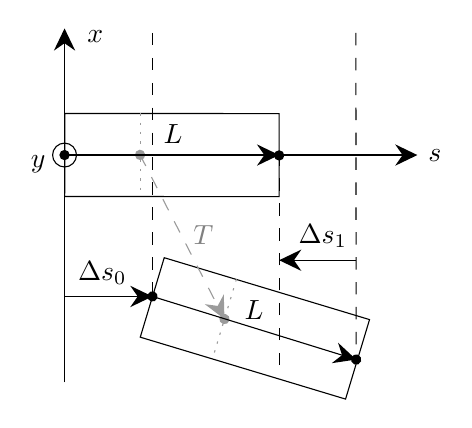
\begin{tikzpicture}[x=0.75pt,y=0.75pt,yscale=-1,xscale=1]
		%Straight Lines [id:da35507818785418455]
		\draw    (127.75,70.82) -- (191.11,70.82) ;
		\draw [shift={(194.11,70.82)}, rotate = 180] [fill={rgb, 255:red, 0; green, 0; blue, 0 }  ][line width=0.08]  [draw opacity=0] (10.72,-5.15) -- (0,0) -- (10.72,5.15) -- (7.12,0) -- cycle    ;
		%Straight Lines [id:da8526813980418886]
		\draw    (24.11,180.32) -- (24.11,12.82) ;
		\draw [shift={(24.11,9.82)}, rotate = 90] [fill={rgb, 255:red, 0; green, 0; blue, 0 }  ][line width=0.08]  [draw opacity=0] (10.72,-5.15) -- (0,0) -- (10.72,5.15) -- (7.12,0) -- cycle    ;
		%Flowchart: Connector [id:dp5359668052415314]
		\draw  [draw opacity=0][fill={rgb, 255:red, 0; green, 0; blue, 0 }  ,fill opacity=1 ] (125,71) .. controls (125,69.62) and (126.12,68.5) .. (127.5,68.5) .. controls (128.88,68.5) and (130,69.62) .. (130,71) .. controls (130,72.38) and (128.88,73.5) .. (127.5,73.5) .. controls (126.12,73.5) and (125,72.38) .. (125,71) -- cycle ;
		%Flowchart: Connector [id:dp7969702218848098]
		\draw  [draw opacity=0][fill={rgb, 255:red, 0; green, 0; blue, 0 }  ,fill opacity=1 ] (64.14,138.06) .. controls (64.63,136.77) and (66.07,136.12) .. (67.36,136.62) .. controls (68.65,137.11) and (69.3,138.55) .. (68.81,139.84) .. controls (68.32,141.13) and (66.87,141.78) .. (65.58,141.29) .. controls (64.29,140.8) and (63.65,139.35) .. (64.14,138.06) -- cycle ;
		%Flowchart: Connector [id:dp09475937969231463]
		\draw  [draw opacity=0][fill={rgb, 255:red, 0; green, 0; blue, 0 }  ,fill opacity=1 ] (162.27,168.45) .. controls (162.77,167.16) and (164.21,166.51) .. (165.5,167) .. controls (166.79,167.49) and (167.44,168.94) .. (166.95,170.23) .. controls (166.45,171.52) and (165.01,172.16) .. (163.72,171.67) .. controls (162.43,171.18) and (161.78,169.74) .. (162.27,168.45) -- cycle ;
		%Shape: Ellipse [id:dp5244406786344289]
		\draw   (20.02,74.86) .. controls (17.78,72.61) and (17.8,68.97) .. (20.06,66.73) .. controls (22.32,64.5) and (25.96,64.52) .. (28.19,66.77) .. controls (30.43,69.03) and (30.41,72.67) .. (28.15,74.91) .. controls (25.89,77.14) and (22.25,77.12) .. (20.02,74.86) -- cycle ;
		%Flowchart: Connector [id:dp7900569932281408]
		\draw  [draw opacity=0][fill={rgb, 255:red, 0; green, 0; blue, 0 }  ,fill opacity=1 ] (21.61,70.82) .. controls (21.61,69.44) and (22.72,68.32) .. (24.11,68.32) .. controls (25.49,68.32) and (26.61,69.44) .. (26.61,70.82) .. controls (26.61,72.2) and (25.49,73.32) .. (24.11,73.32) .. controls (22.72,73.32) and (21.61,72.2) .. (21.61,70.82) -- cycle ;

		%Flowchart: Connector [id:dp1702286240852332]
		\draw  [draw opacity=0][fill={rgb, 255:red, 155; green, 155; blue, 155 }  ,fill opacity=1 ] (58.01,70.93) .. controls (57.91,69.55) and (58.94,68.36) .. (60.32,68.26) .. controls (61.7,68.16) and (62.89,69.19) .. (62.99,70.57) .. controls (63.09,71.95) and (62.06,73.14) .. (60.68,73.24) .. controls (59.3,73.34) and (58.11,72.31) .. (58.01,70.93) -- cycle ;
		%Shape: Rectangle [id:dp5029720108971986]
		\draw   (24.19,50.8) -- (127.5,50.84) -- (127.49,90.84) -- (24.18,90.8) -- cycle ;
		%Straight Lines [id:da5919731693823477]
		\draw [color={rgb, 255:red, 155; green, 155; blue, 155 }  ,draw opacity=1 ] [dash pattern={on 0.84pt off 2.51pt}]  (60.5,50.75) -- (60.5,90.75) ;
		%Flowchart: Connector [id:dp7156618154401919]
		\draw  [draw opacity=0][fill={rgb, 255:red, 155; green, 155; blue, 155 }  ,fill opacity=1 ] (98.71,149.3) .. controls (99.02,147.95) and (100.35,147.1) .. (101.7,147.4) .. controls (103.05,147.7) and (103.9,149.04) .. (103.59,150.39) .. controls (103.29,151.74) and (101.96,152.58) .. (100.61,152.28) .. controls (99.26,151.98) and (98.41,150.65) .. (98.71,149.3) -- cycle ;
		%Shape: Rectangle [id:dp06216288058859021]
		\draw   (72.14,120.28) -- (171.05,150.1) -- (159.5,188.4) -- (60.59,158.57) -- cycle ;
		%Straight Lines [id:da15643091065704995]
		\draw [color={rgb, 255:red, 155; green, 155; blue, 155 }  ,draw opacity=1 ] [dash pattern={on 0.84pt off 2.51pt}]  (106.92,130.69) -- (95.39,168.99) ;
		%Straight Lines [id:da3239479052474509]
		\draw [color={rgb, 255:red, 155; green, 155; blue, 155 }  ,draw opacity=1 ] [dash pattern={on 4.5pt off 4.5pt}]  (60.5,70.75) -- (99.78,147.18) ;
		\draw [shift={(101.15,149.84)}, rotate = 242.8] [fill={rgb, 255:red, 155; green, 155; blue, 155 }  ,fill opacity=1 ][line width=0.08]  [draw opacity=0] (10.72,-5.15) -- (0,0) -- (10.72,5.15) -- (7.12,0) -- cycle    ;
		%Straight Lines [id:da4836988544272087]
		\draw  [dash pattern={on 4.5pt off 4.5pt}]  (66.47,12) -- (66.47,138.95) ;
		%Straight Lines [id:da5330246211677179]
		\draw  [dash pattern={on 4.5pt off 4.5pt}]  (127.5,172) -- (127.5,71) ;
		%Straight Lines [id:da5582054958236305]
		\draw  [dash pattern={on 4.5pt off 4.5pt}]  (164.47,12) -- (164.61,169.34) ;
		%Straight Lines [id:da2986734039407184]
		\draw    (23.97,138.95) -- (63.47,138.95) ;
		\draw [shift={(66.47,138.95)}, rotate = 180] [fill={rgb, 255:red, 0; green, 0; blue, 0 }  ][line width=0.08]  [draw opacity=0] (10.72,-5.15) -- (0,0) -- (10.72,5.15) -- (7.12,0) -- cycle    ;
		%Straight Lines [id:da8950058864242387]
		\draw    (66.47,138.95) -- (161.74,168.45) ;
		\draw [shift={(164.61,169.34)}, rotate = 197.2] [fill={rgb, 255:red, 0; green, 0; blue, 0 }  ][line width=0.08]  [draw opacity=0] (10.72,-5.15) -- (0,0) -- (10.72,5.15) -- (7.12,0) -- cycle    ;
		%Straight Lines [id:da776090670545246]
		\draw    (164.61,121.5) -- (130.5,121.5) ;
		\draw [shift={(127.5,121.5)}, rotate = 360] [fill={rgb, 255:red, 0; green, 0; blue, 0 }  ][line width=0.08]  [draw opacity=0] (10.72,-5.15) -- (0,0) -- (10.72,5.15) -- (7.12,0) -- cycle    ;
		%Straight Lines [id:da6954530061787899]
		\draw    (24.11,70.82) -- (124.5,70.82) ;
		\draw [shift={(127.5,70.82)}, rotate = 180] [fill={rgb, 255:red, 0; green, 0; blue, 0 }  ][line width=0.08]  [draw opacity=0] (10.72,-5.15) -- (0,0) -- (10.72,5.15) -- (7.12,0) -- cycle    ;

		% Text Node
		\draw (33.86,9.72) node [anchor=north west][inner sep=0.75pt]    {$x$};
		% Text Node
		\draw (198.11,66.72) node [anchor=north west][inner sep=0.75pt]    {$s$};
		% Text Node
		\draw (6.61,69.72) node [anchor=north west][inner sep=0.75pt]    {$y$};
		% Text Node
		\draw (84.86,103.47) node [anchor=north west][inner sep=0.75pt]  {\textcolor{gray}{$T$}};
		% Text Node
		\draw (70.61,54.9) node [anchor=north west][inner sep=0.75pt]    {$L$};
		% Text Node
		\draw (109.61,139.9) node [anchor=north west][inner sep=0.75pt]    {$L$};
		% Text Node
		\draw (29.36,120.9) node [anchor=north west][inner sep=0.75pt]    {$\Delta s_{0}$};
		% Text Node
		\draw (135.61,102.9) node [anchor=north west][inner sep=0.75pt]    {$\Delta s_{1}$};
	\end{tikzpicture}
	\caption{Visualization of the $s$-coordinate transformations without correction.}\label{fig:no-s-no-zeta-correction}
\end{figure}

In the visualization in Fig.~\ref{fig:no-s-no-zeta-correction} we can see the different $s$-coordinate updates taking place when we track through a misalignment: in particular, we can see that the total path of the particle traveled, should SShift be simply a drift, is $\Delta s = \Delta s_0 + L + \Delta s_1$.
Clearly, $\Delta s_0 \neq -\Delta s_1$, and so the path length changes between the aligned and misaligned element.
However, what we desire is the opposite, i.e.~that the path length does not change: it is inconvenient to have the length of our accelerator change due to a misalignment.
Therefore, the simplest correction we can make in this instance is to disregard the update of the $s$ coordinate in our drift/$s$-shift.

A further correction needs to be made with respect to the $\zeta$ coordinate.
Since $\zeta$ is related to the path length by $\zeta = s - \beta_0 c t$, and since, in our setup, the synchronous particle arrival time is not expected to change between the normal and misaligned entry to the element, we expect that $\Delta \zeta = \Delta s$ between those two points.
However, as we have already established for our correction of $s$, we expect the $s$ coordinate to be unchanged, so we can adjust $\zeta$ in exactly the same fashion as we do $s$:

\[
	\text{SShift}(\Delta s) := ( \text{DriftExact}(\Delta s),\;\; s \leftarrow s - \Delta s,\;\; \zeta \leftarrow \zeta - \Delta s ).
\]


% \section{Other notes}

% The rotation direction conventions differ between the MAD-X survey coordinate system and the beam coordinate system, in that the $y$-rotation of the beam is opposite to the one described by YRot in the tracking procedures above. This sign difference is taken into account in the Xsuite implementation.




\chapter{Linear optics}
\label{opt}
We define $z$ as the vector of $2 k$ coordinates,
\begin{align}\label{opt:eqn:1}
z&=(z_1,\ldots,z_{2k})^T=(x-x_0,p_x-p_{x0},y-y_0,p_y-p_{y0},\zeta-\zeta_0,p_\zeta-p_{\zeta0})^T
\end{align}
One can define linear transfer maps (e.g. $R_{1\to 2}$ that propagates coordinates between two points $s_1$, $s_2$) and the one-turn map (e.g. $R_1$ that combines the effects for one turn starting from $s_1$):
\begin{align}\label{opt:eqn:2}
z(s_2)&= R_{1\to 2} z(s_1) & z(C+s_1) &= R_1 z(s_1).
\end{align}
In the following we will describe the optics calculation based on the Ripken formalism described in \cite{willeke88}. A good summary is also given in the MAD8 physics manual \cite{mad8phys}.

\section{Linear normal form}
\label{opt:sec:1}
Since the matrices derive from symplectic maps, the eigenvalue spectrum of the one-turn map $R$ consists of 2$k$ distinct eigenvalues and linearly independent eigenvectors. In addition, for the motion to be stable the eigenvalues $\lambda_k^{\pm}$ with eigenvectors $v_k^{\pm}$ have to be complex \cite{willeke88}:
\begin{align}
R v_k^\pm  =  \lambda_k^\pm v_k^\pm, \ k=1,\ldots, 3 \\
v_k^+=(v_k^-)^*, \quad \lambda_k^+=(\lambda_k^-)^*, \quad |\lambda_k^{\pm}|=1
\end{align}
As the eigenvectors are linearly independent, $R$ can be diagonalized with
\begin{align}
R &= V \Lambda V^{-1},
\end{align}
where $V$ consists of the eigenvectors and $\Lambda$ of the eigenvalues:
\begin{align}
V=&\left(
\begin{array}{cccc}
v^+_{1,1} & v^-_{1,1} & \cdots & v^-_{3,1}\\
v^+_{1,2} & v^-_{1,2} & \cdots & v^-_{3,2}\\
\vdots    & \vdots    & \vdots & \vdots \\
\end{array}
\right)  &
\Lambda=&\left(
\begin{array}{cccc}
\lambda^+_1 &    & &\\
& \lambda^-_1 & &\\
& & \ddots & \\
& & & \lambda^-_3
\end{array}
\right)
\end{align}
for which $v^{\pm}_{i,j}$ is the component $j$ of eigenvector $v_i^{\pm}$.

The same calculation can be carried out with real numbers by the following definitions:
\begin{align}\
v_k^\pm &= a_k\pm ib_k, & \lambda_k^\pm &= \cos \mu_k \pm i \sin \mu_k, &
\mu_k, a_k, b_k \in \mathbb{R}
\end{align}
such that:
\begin{align}\label{eq:lin_norm_form}
R=&W R_{\mathrm{rot}} W^{-1}
\end{align}
with
\begin{align}
R_{\mathrm{rot}}=R_{\mathrm{rot}}(\mu_k)=&\left(
\begin{array}{ccccc}
\cos \mu_1 & \sin \mu_1  &  & &\\
-\sin \mu_1 & \cos \mu_1 &  & &\\
&    & \ddots & &\\
& & & \cos \mu_3 & \sin \mu_3 \\
& & & -\sin \mu_3 & \cos \mu_3 \\
\end{array}
\right), \\
W=&\left(
\begin{array}{ccccc}
a_{1,1} & b_{1,1} & \cdots & a_{3,1} & b_{3,1} \\
a_{1,2} & b_{1,2} & \cdots & a_{3,2} & b_{3,2} \\
\vdots    & \vdots    & \vdots & \vdots\\
a_{1,6} & b_{1,6} & \cdots & a_{3,6} & b_{3,6} \\
\end{array}
\right)
\end{align}
Equation~\ref{eq:lin_norm_form} is called the linear normal form of the one-turn map $R$.
The matrix $R_{\mathrm{rot}}$ describes a rotation in the 3 planes by angles $\mu_k$.

Usually $\mu_k$ is written as $\mu_k=2\pi Q_k$, where $Q_k$ is then the tune of the mode $k$.
By convention, the eigenvectors and values are normalized, sorted and rotated so that the following three conditions are fulfilled:
\begin{enumerate}
\item Plane 1 is associated with the horizontal, plane 2 with the vertical and plane 3 with the longitudinal plane. This is achieved by first normalizing the eigenvectors $v_k^{\pm}$ and then sorting them so that:
\begin{align}\label{opt:eqn:2:1}
|v_{j,2j-1}^{+}| =|v_{j,2j-1}^{-}| = \max_{k=1,2,3} v_{k,j}, \quad j=1,\ldots, 3
\end{align}
\item The eigenvectors are then rotated with a phase term $\psi_k$
\begin{align}
v_k& \to v_k \exp(i \psi_k)
\end{align}
such that
\begin{align}\label{opt:eqn:2:2}
\mathrm{angle}(v_{k,2k-1}^{+})=0 \leftrightarrow \psi_k=-\mathrm{angle}(v_{k,2k-1}^{+})
\end{align}
In real space, Eqns.~\ref{opt:eqn:2:1} and \ref{opt:eqn:2:2} then become equivalent to:
\begin{align}
|a_{j,2j-1}| &=\max_{k=1,2,3} |a_{k,j}|,& b_{j,2 j-1}&=0, & j=1,\ldots, 3
\end{align}
This has the effect that a particle with $x=0$ is transformed to $\tilde x$ in the normalized phase space.
\item The sign of $b_{k,j}$ is fixed by the symplectic condition on $W$
\begin{align}
W^T S W = S
\end{align}
with $S$ defined as
\begin{align}
S&=\left(
\begin{array}{cccccc}
0 & 1 & 0 & 0 & 0 & 0\\
-1 & 0 & 0 & 0 & 0 & 0\\
0 & 0 & 0 & 1 & 0 & 0\\
0 & 0 & -1 & 0 & 0 & 0\\
0 & 0 & 0 & 0 & 0 & 1\\
0 & 0 & 0 & 0 & -1 & 0
\end{array}
\right)
\label{eq:symplectic_matrix}
\end{align}
which is equivalent to:
\begin{align}\label{opt:eqn:2:3}
a_k^T \cdot S \cdot b_k &=1, \quad b_k^T \cdot S \cdot a_k =-1, & \text{ for } k=l\nonumber\\
a_k^T \cdot S \cdot b_l &=0, & \text{ for }  k\not=l\\
a_k^T \cdot S \cdot a_l &=0, \quad b_k^T \cdot S \cdot b_l =0,  & k,l=1,\ldots,3 \nonumber
\end{align}
Eqn.~\ref{opt:eqn:2:3} yields that in phase space $a_k$ is thus obtained by an anticlockwise rotation of $b_k$ by $\pi/2$ and a scaling of its length with $|a_k|=\frac{1}{|b_k|}$.
\end{enumerate}

We will show in the following that in the normalized phase space the propagation of particle coordinates $z(s)$ from $s_1$ to $s_2$ is just a rotation by an angle $\phi_k$ in the $k=1,\ldots,3$ planes, while the amplitude $I_k$ and initial phase $\phi_{k,0}$ stay constant, explicitly $z(s)$ is then given by:
\begin{align}\label{opt:eqn:3:3}
z(s)=\sum_{k=1}^3 \sqrt{2I_k}\left(
a_k(s) \cos \left(\phi_{k,0} + \phi_k(s)\right) -
b_k(s) \sin \left(\phi_{k,0} + \phi_k(s)\right)
\right)
\end{align}
and
\begin{align}
z(s_2)&=W(s_2)R_{\mathrm{rot}}(\phi_k)W(s_1)^{-1}z(s_1), \\
&\hspace{30pt} \text{ with } \phi_k=\phi_k(s_2)-\phi_k(s_1)\nonumber
\end{align}
This implies that one turn is simply a rotation by $\phi_k=2\pi Q_k$ where $Q_k$ is the tune of the mode $k$. In the transverse plane the tune ($Q_{I,II}$) is usually positive and the particles rotate clockwise, while in the longitudinal plane the tune ($Q_{III}$) is negative above $\gamma_T$ leading to an anticlockwise rotation.

For the derivation the following steps are needed:
\begin{enumerate}
\item The effect of one turn on the normalized variable $\tilde z(s)=W^{-1}(s) z(s)$ is a rotation:
\begin{align}\label{opt:eqn:3:1}
\tilde z(C+s) = W^{-1}z(s+C)\overset{(\rm Eqn.\ref{eq:lin_norm_form})}{=}W^{-1}W R_{\mathrm{rot}} W^{-1}z(s)= R_{\mathrm{rot}}\tilde z(s),
\end{align}
As $R$ and $R_{\mathrm{rot}}$ are symplectic, $W$ is also symplectic, and its inverse is thus given by $S^{-1}W^{T}S$, explicitly:
\begin{align}
W^{-1}&=
\left(
\begin{array}{cccccc}
b_{12} & - b_{11} &   b_{14} & - b_{13} &   b_{16} & - b_{15}\\
- a_{12} &   a_{11} & - a_{14} &   a_{13} & - a_{16} &   a_{15}\\
b_{22} & - b_{21} &   b_{24} & - b_{23} &   b_{26} & - b_{25}\\
- a_{22} &   a_{21} & - a_{24} &   a_{23} & - a_{26} &   a_{25}\\
b_{32} & - b_{31} &   b_{34} & - b_{33} &   b_{36} & - b_{35}\\
- a_{32} &   a_{31} & - a_{34} &   a_{33} & - a_{36} &   a_{35}\\
\end{array}
\right)
\label{eq:winv}
\end{align}
\item The one-turn map and $W$-matrix can be propagated from $s_1$ to $s_2$ by
\begin{align}
R_2&=R_{1 \to 2} R_1 R^{-1}_{1 \to 2}  &
W_2&=R_{1 \to 2} W_1
\end{align}
As Eqn.~\ref{opt:eqn:3:1} represents a similarity transformation, the eigenvalues are thus independent of the position $s$ and as the rotation matrix $R_{\mathrm{rot}}$ consists of the eigenvalues of $R$, the angle of the rotation $\mu_k=2\pi Q_k$ is thus also independent of $s$.

\item As Eqn.~\ref{eq:lin_norm_form} represents a basis transformation from the standard $\mathbb{R}^2$ basis to the eigenvector basis, the vectors $a_k$ and $b_k$ are projected onto (Eqn.~\ref{opt:eqn:2:3}):
\begin{align}\label{opt:eqn:3:2}
\tilde a_1=W^{-1}a_1&=-SW^TSa_1\nonumber\\
&=-S(a_1Sa_1,b_1Sa_1,\ldots,b_3Sa_1)^T=(1,0,\ldots,0)\nonumber\\
\tilde b_1=W^{-1}b_1&=-SW^TSb_1\nonumber\\
&=-S(a_1Sb_1,b_1Sb_1,\ldots,b_3Sb_1)^T=(0,1,\ldots,0)\\
\cdots & \nonumber\\
\tilde b_3=W^{-1}b_3&=-SW^TSb_3\nonumber\\
&=-S(a_1Sb_3,b_1Sb_3,\ldots,b_3Sb_3)^T=(0,0,\ldots,1)\nonumber
\end{align}
in the normalized phase space.
\item From Eqn.~\ref{opt:eqn:3:1} it follows that the amplitude $I_k$ and initial phase $\phi_{k0}$ of $\tilde z=W^{-1}z=(\tilde z_{a_1},\tilde z_{b_1},\ldots,\tilde z_{b_3})$
\begin{align}
I_k&=\frac{(\tilde z_{a_k})^2 +(\tilde z_{b_k})^2}{2}, \quad k=1,\ldots,3\label{opt:eqn:20a}\\
\tan\phi_{k0}&=-\frac{\tilde z_{b_k}}{\tilde z_{a_k}} \label{opt:eqn:20b}
\end{align}
are constants of the motion.
%, which is illustrated in Fig.~\ref{opt:fig:1}.
%\begin{figure}[h]
%	\centering
%	\includegraphics{normalized_phase_space_cropped.pdf}
%	\caption{Normalized phase space.\label{opt:fig:1}}
%\end{figure}
The initial phase is defined with a minus sign in view of the definition of the Twiss parameters, where the initial phase is then added (and not subtracted) to the phase advance. The components of $\tilde z$ are then explicitly given by:
\begin{align}
\tilde z_{a_k}&= \sum_{j=1}^3  b_{k,2j} z_{2j-1}- b_{k,2j-1} z_{2j}, \quad k=1,\ldots,3\\
\tilde z_{b_k}&= \sum_{j=1}^3 a_{k,2j-1} z_{2j}- a_{k,2j} z_{2j-1}, \quad k=1,\ldots,3.
\end{align}
An arbitrary vector $z(s)$ can thus be written in the following form:
\begin{align}
 z(s)&=W(s)\tilde z(s)\nonumber\\
 &=W(s)\left(\sum_{k=1}^{3}\tilde z_{a_k}\tilde a_k + \tilde z_{b_k}\tilde b_k\right)\nonumber\\
 &=\sum_{k=1}^{3}\tilde z_{a_k}W(s)\tilde a_k + \tilde z_{b_k}W(s)\tilde b_k\overset{\rm Eqn.~\ref{opt:eqn:3:2}}{=}\sum_{k=1}^{3}\tilde z_{a_k}a_k + \tilde z_{b_k}b_k\nonumber\\
 &\overset{\rm Eqns.~\ref
 	{opt:eqn:20a},\ref{opt:eqn:20b}}=\sum_{k=1}^{3}\sqrt{2I_k}\left(a_k\cos{\phi_{k0}}-b_k\sin{\phi_{k0}}\right)
\end{align}
\end{enumerate}

\section{Twiss parameters}
\label{opt:sec:4}
In the following the parameter $k$ will always be used for the mode $k$ and the parameter
$j=1,2,3$ for the horizontal ($x,p_x$), vertical ($y,p_y$) and longitudinal plane
$(\zeta,p_\zeta)$ in the phase space. $z_{2j-1}$ then stands for the coordinates $(x,y,\zeta$)
and $z_{2j}$ for $(p_x,_y,p_\zeta$).

The Twiss parameters can be introduced by writing the components of the eigenvector basis
$(a_k(s),b_k(s))$ as the product of two envelope functions $\sqrt{\beta_{k,j}(s)}$,
$\sqrt{\gamma_{k,j}(s)}$ and phase functions $\phi_{k,j}(s)$, $\bar\phi_{k,j}(s) = \phi_{k,j}(s) - \arctan(1/\alpha_{k,j})$,
also called Twiss parameters or lattice functions, with
\begin{align}
a_{k,2j-1}(s)&=\sqrt{\beta_{k,j}(s)}\cos{\phi_{k,j}(s)},\nonumber\\ b_{k,2j-1}(s)&=\sqrt{\beta_{k,j}(s)}\sin{\phi_{k,j}(s)}, \ k,j=1,\ldots,3, \label{opt:eqn:4:1}\\
a_{k,2j}(s)&=\sqrt{\gamma_{k,j}(s)}\cos{\bar\phi_{k,j}(s)}, \nonumber\\
b_{k,2j}(s)&=\sqrt{\gamma_{k,j}(s)}\sin{\bar\phi_{k,j}(s)}, \ k,j=1,\ldots,3 \label{opt:eqn:4:2}
\end{align}
where $\beta_{k,j}(s), \alpha_{k,j}(s), \gamma_{k,j}(s)$ represent the projection of the ellipse of mode $k$ on the plane of coordinates $z_{2k-1}-z_{2k}$.
%(see Fig.~\ref{opt:fig:2})
%\begin{figure}[!ht]
%	\centering
%	\includegraphics[width=1.0\linewidth]{ripken_phase_space_ellipse.png}
%	\caption{Projection of lattice function in the $z-z'$ plane.\label{opt:fig:2}}
%\end{figure}

Using Eqns.~\ref{opt:eqn:3:3}, \ref{opt:eqn:4:1}, \ref{opt:eqn:4:2} and $\cos(x+y)=\cos x\cos y-\sin x\sin y$, the coordinates $z(s)$ can be expressed by:
\begin{align}
z_{2j-1}(s)&=\sum_{k=1}^3 \sqrt{2I_k
\beta_{k,j}(s)}\cos{(\phi_{k,j}(s)+\phi_{k,0})}\\
z_{2j}(s)&=\sum_{k=1}^3 \sqrt{2I_k
\gamma_{k,j}(s)}\cos{(\bar\phi_{k,j}(s)+\phi_{k,0})}, \ j=1,\ldots,3
\end{align}
Conversely the lattice functions can also be expressed by $a_k$ and $b_k$ with
\begin{align}
\beta_{k,j}(s)&=a_{k,2j-1}(s)^2 +b_{k,2j-1}(s)^2 \\
\alpha_{k,j}(s)&=- a_{k,2j-1}(s)a_{k,2j}(s) -b_{k,2j-1}(s)b_{k,2j}(s) \\
\gamma_{k,j}(s)&=a_{k,2j}(s)^2 +b_{k,2j}(s)^2,
\end{align}
The well-known relations between the lattice functions
\begin{align}
\sum_{j=1}^3\beta_{k,j}\phi_{k,j}'&=1 \\
\gamma_{k,j}&=\frac{\beta_{k,j}^2\phi_{k,j}'^2+\alpha_{k,j}^2}{\beta_{k,j}}, \text{ with  }\\
\alpha_{k,j}&:=-\frac{1}{2}\beta_{k,j}'
\end{align}
can then be derived with the help of the normalization condition (Eqn.~\ref{opt:eqn:2:3})
\begin{align}
a_k^TSb_k=1
\end{align}
by the following steps:
\begin{enumerate}
\item As $x'=\frac{dx}{ds},\ y'=\frac{dy}{ds}$ the following relations hold also for $a_k$ and $b_k$:
\begin{align}
a_{k,2j}=a_{k,2j-1}'&=\frac{d}{ds}(a_{k,2j-1}), \\
b_{k,2j}=b_{k,2j-1}'&=\frac{d}{ds}(b_{k,2j-1}),\ k,j=1,\ldots,3
\end{align}
\item The normalization condition Eqn.~\ref{opt:eqn:2:3} can then be written as
\begin{align}
a_k^TSb_k&=\sum_{j=1}^3\sqrt{\beta_{k,j}}\cos{\phi_{k,j}}\left(\sqrt{\beta_{k,j}}\sin{\phi_{k,j}}\right)'\nonumber\\
& \qquad -\left(\sqrt{\beta_{k,j}}\cos{\phi_{k,j}}\right)'\sqrt{\beta_{k,j}}\sin{\phi_{k,j}}\nonumber\\
&=\sum_{j=1}^3\beta_{k,j}\phi_{k,j}'\nonumber\\
&=1 \label{opt:eqn:4:3}
\end{align}
Note that Eqn.~\ref{opt:eqn:4:3} yields the following relation between the phase advance $\phi$ and $\beta$ in 2D:
\begin{align}
\phi(s)=\phi(0)+\int_{s_0}^s\frac{1}{\beta(\bar s)}d\bar s
\end{align}
\item Using the abbreviation $\alpha_{k,j}:=-\frac{1}{2}\beta_{k,j}$, one finds for each mode $k$ and plane $j$
\begin{align}
\sqrt{\gamma_{k,j}}\cos{\phi_{k,j}}&=a_{k,2j}=a_{k,2j-1}'=(\sqrt{\beta_{k,j}}\cos{\phi_{k,j}})' &\quad (1)\nonumber\\
\sqrt{\gamma_{k,j}}\sin{\phi_{k,j}}&=b_{k,2j}=b_{k,2j-1}'=(\sqrt{\beta_{k,j}}\sin{\phi_{k,j}})' &\quad (2)\nonumber\\
\overset{(1)^2+(2)^2}{\Rightarrow} \gamma_{k,j}&=\frac{\beta_{k,j}^2\phi_{k,j}'^2+\alpha_{k,j}^2}{\beta_{k,j}}, \quad k,j=1,\ldots,3 &
\end{align}
which simplifies in the 2D case to:
\begin{align}
\gamma\overset{\rm Eqn.~\ref{opt:eqn:4:3}}{=}\frac{1+\alpha^2}{\beta}
\end{align}
\end{enumerate}

\section{Transformation to normalized coordinates}

The $W$ matrix can be used to transform normalized coordinates into physical
coordinates relative to the closed orbit and vice versa:

\begin{equation}
\left(\begin{array}{l}
x - x_0\\
p_x - p_{x0}\\
y - y_0\\
p_y - p_{y0}\\
\zeta - \zeta_0\\
p_\zeta - p_{\zeta0}
\end{array}\right)
=
W
\left(\begin{array}{l}
\hat{x} \\
\hat{p}_x \\
\hat{y} \\
\hat{p}_y \\
\hat{\zeta} \\
\hat{p}_\zeta
\end{array}\right)
=
W
\left(\begin{array}{l}
\sqrt{\varepsilon_x} \tilde{x} \\
\sqrt{\varepsilon_x} \tilde{p}_x \\
\sqrt{\varepsilon_y} \tilde{y} \\
\sqrt{\varepsilon_y} \tilde{p}_y \\
\sqrt{\varepsilon_\zeta} \tilde{\zeta} \\
\sqrt{\varepsilon_\zeta} \tilde{p}_\zeta
\end{array}\right)
\label{eq:norm_coord}
\end{equation}
where the subscript $0$ denotes the closed orbit at the observation point, and
\begin{equation}
\left(\begin{array}{llllll}\tilde{x} & \tilde{p}_x & \tilde{y} & \tilde{p}_y & \tilde{\zeta} & \tilde{p}_\zeta\end{array}\right)
\end{equation}
are normalized coordinates in sigmas and $\varepsilon_x$, $\varepsilon_y$ and $\varepsilon_\zeta$ are the geometric emittances.

\section{Covariance matrix}
\label{opt:sec:covariance}

The beam covariance matrix is defined from the central second moments of the
phase-space coordinates
\begin{equation}
z =
\left(\begin{array}{llllll}
x & p_x & y & p_y & \zeta & p_\zeta
\end{array}\right)^T
\end{equation}
as
\begin{equation}
\Sigma = \left<\left(z-\left<z\right>\right)
\left(z-\left<z\right>\right)^T\right>.
\label{eq:covariance_definition}
\end{equation}
The subtraction of the centroid makes $\Sigma$ independent of the closed-orbit
offset of the distribution.

\subsection{Normal-mode emittances}

Let
\begin{equation}
\hat{z} =
\left(\begin{array}{llllll}
\hat{x} & \hat{p}_x & \hat{y} & \hat{p}_y &
\hat{\zeta} & \hat{p}_\zeta
\end{array}\right)^T
\end{equation}
be the normalized coordinates appearing in Eq.~\ref{eq:norm_coord}, so that
$z-z_0=W\hat{z}$, where $z_0$ is the closed orbit. We define
$\Delta\hat{z}=\hat{z}-\left<\hat{z}\right>$ and group the normalized
coordinates by mode as
\begin{equation}
\Delta\hat{z}_x =
\left(\begin{array}{c}
\Delta\hat{x}\\
\Delta\hat{p}_x
\end{array}\right),\quad
\Delta\hat{z}_y =
\left(\begin{array}{c}
\Delta\hat{y}\\
\Delta\hat{p}_y
\end{array}\right),\quad
\Delta\hat{z}_\zeta =
\left(\begin{array}{c}
\Delta\hat{\zeta}\\
\Delta\hat{p}_\zeta
\end{array}\right).
\end{equation}
For a beam matched to the linear optics, the particles are distributed in each
normal-mode plane with no preferred betatron phase. We write the
centroid-subtracted coordinates of mode $k$ as
\begin{equation}
\Delta\hat{q}_k = A_k \cos\phi_k,\qquad
\Delta\hat{p}_k = -A_k \sin\phi_k,
\end{equation}
where $(\Delta\hat{q}_k,\Delta\hat{p}_k)$ stands for
$(\Delta\hat{x},\Delta\hat{p}_x)$,
$(\Delta\hat{y},\Delta\hat{p}_y)$, or
$(\Delta\hat{\zeta},\Delta\hat{p}_\zeta)$. If the phase distribution is uniform
and independent of the amplitude, then
\begin{equation}
\left<\cos^2\phi_k\right> = \left<\sin^2\phi_k\right> = \frac{1}{2},
\qquad
\left<\sin\phi_k\cos\phi_k\right> = 0,
\end{equation}
and the covariance block of mode $k$ is
\begin{align}
C_k
&= \left<\Delta\hat{z}_k\Delta\hat{z}_k^T\right>\nonumber\\
&=
\left(\begin{array}{cc}
\left<A_k^2\cos^2\phi_k\right> &
-\left<A_k^2\sin\phi_k\cos\phi_k\right>\\
-\left<A_k^2\sin\phi_k\cos\phi_k\right> &
\left<A_k^2\sin^2\phi_k\right>
\end{array}\right)\nonumber\\
&=
\frac{\left<A_k^2\right>}{2}
\left(\begin{array}{cc}
1 & 0\\
0 & 1
\end{array}\right).
\end{align}
Defining $\varepsilon_k=\left<A_k^2\right>/2$, each normal-mode block is
$C_k=\varepsilon_k I$. If the normal-mode variables are statistically
independent, then the cross-covariances between different modes vanish:
\begin{equation}
\left<\Delta\hat{z}_j\Delta\hat{z}_k^T\right> = 0,
\qquad j\ne k.
\end{equation}
It follows that the covariance of the normalized coordinates is
\begin{equation}
\left<\Delta\hat{z}\Delta\hat{z}^T\right> = E,
\label{eq:covariance_normalized_coordinates}
\end{equation}
with
\begin{equation}
E =
\left(\begin{array}{cccccc}
\varepsilon_x & 0 & 0 & 0 & 0 & 0\\
0 & \varepsilon_x & 0 & 0 & 0 & 0\\
0 & 0 & \varepsilon_y & 0 & 0 & 0\\
0 & 0 & 0 & \varepsilon_y & 0 & 0\\
0 & 0 & 0 & 0 & \varepsilon_\zeta & 0\\
0 & 0 & 0 & 0 & 0 & \varepsilon_\zeta
\end{array}\right).
\label{eq:covariance_emittance_matrix}
\end{equation}
Since $W$ is a linear transformation, Eq.~\ref{eq:norm_coord} gives
\begin{equation}
z-\left<z\right> = W\left(\hat{z}-\left<\hat{z}\right>\right).
\end{equation}
Substituting this expression in Eq.~\ref{eq:covariance_definition} gives
\begin{align}
\Sigma
&= \left< W\left(\hat{z}-\left<\hat{z}\right>\right)
\left(W\left(\hat{z}-\left<\hat{z}\right>\right)\right)^T \right>\nonumber\\
&= W\left<\left(\hat{z}-\left<\hat{z}\right>\right)
\left(\hat{z}-\left<\hat{z}\right>\right)^T\right>W^T\nonumber\\
&= W E W^T.
\label{eq:sigma_wewt}
\end{align}
Since $W$ is symplectic,
\begin{equation}
W^T S W = S,
\end{equation}
and therefore
\begin{equation}
W^T S = S W^{-1}.
\end{equation}
Multiplying Eq.~\ref{eq:sigma_wewt} by $S$ on the right gives
\begin{equation}
\Sigma S = W E W^T S = W E S W^{-1}.
\label{eq:sigma_s_similarity}
\end{equation}
Thus $\Sigma S$ is obtained from $ES$ by a change of basis with matrix $W$.
This implies that the two matrices have the same eigenvalues: if $q$ is an
eigenvector of $ES$ with eigenvalue $\lambda$, then
\begin{equation}
\Sigma S\, Wq = W E S W^{-1} Wq = W E S q = \lambda Wq.
\end{equation}
Therefore $Wq$ is an eigenvector of $\Sigma S$ with the same eigenvalue
$\lambda$. Combining Eqs.~\ref{eq:covariance_emittance_matrix} and
\ref{eq:symplectic_matrix} gives
\begin{equation}
E S =
\left(\begin{array}{cccccc}
0 & \varepsilon_x & 0 & 0 & 0 & 0\\
-\varepsilon_x & 0 & 0 & 0 & 0 & 0\\
0 & 0 & 0 & \varepsilon_y & 0 & 0\\
0 & 0 & -\varepsilon_y & 0 & 0 & 0\\
0 & 0 & 0 & 0 & 0 & \varepsilon_\zeta\\
0 & 0 & 0 & 0 & -\varepsilon_\zeta & 0
\end{array}\right),
\end{equation}
which is block diagonal, with one block
\begin{equation}
\left(\begin{array}{cc}
0 & \varepsilon_k\\
-\varepsilon_k & 0
\end{array}\right)
\end{equation}
for each normal mode $k=x,y,\zeta$. Each block has eigenvalues
$\pm i\varepsilon_k$. The eigenvalues of $ES$ in normalized coordinates, and
equivalently of $\Sigma S$ in physical coordinates, are therefore
\begin{equation}
\lambda_k^\pm(ES) = \lambda_k^\pm(\Sigma S) = \pm i \varepsilon_k.
\label{eq:emittance_from_sigma_s}
\end{equation}
The quantities $\varepsilon_k$ are called \textbf{normal-mode emittances}.
Their relation to the action variables is discussed in the following section.

\subsection{Eigenvectors of the covariance matrix}
\label{opt:sec:covariance_eigenvectors}

The eigenvectors of $\Sigma S$ are the same eigenvectors as those of the
one-turn matrix $R$. This can be seen mode by mode. First work in normalized
coordinates, where both $R_{\mathrm{rot}}$ and $ES$ are block diagonal. Let
$q_k^+$ be the vector whose only non-zero normal-mode block is
\begin{equation}
\left(\begin{array}{c}
1\\
i
\end{array}\right)
\end{equation}
in plane $k$. In this plane, the corresponding block of $R_{\mathrm{rot}}$ is
\begin{equation}
\left(\begin{array}{cc}
\cos \mu_k & \sin \mu_k\\
-\sin \mu_k & \cos \mu_k
\end{array}\right),
\end{equation}
and
\begin{equation}
\left(\begin{array}{cc}
\cos \mu_k & \sin \mu_k\\
-\sin \mu_k & \cos \mu_k
\end{array}\right)
\left(\begin{array}{c}
1\\
i
\end{array}\right)
=
\left(\begin{array}{c}
\cos \mu_k+i\sin \mu_k\\
-\sin \mu_k+i\cos \mu_k
\end{array}\right)
=
\exp(i\mu_k)
\left(\begin{array}{c}
1\\
i
\end{array}\right).
\end{equation}
Therefore $R_{\mathrm{rot}} q_k^+ = \exp(i\mu_k)q_k^+$. The corresponding block of $ES$ is
\begin{equation}
\left(\begin{array}{cc}
0 & \varepsilon_k\\
-\varepsilon_k & 0
\end{array}\right),
\end{equation}
and
\begin{equation}
\left(\begin{array}{cc}
0 & \varepsilon_k\\
-\varepsilon_k & 0
\end{array}\right)
\left(\begin{array}{c}
1\\
i
\end{array}\right)
=
\left(\begin{array}{c}
i\varepsilon_k\\
-\varepsilon_k
\end{array}\right)
=
i\varepsilon_k
\left(\begin{array}{c}
1\\
i
\end{array}\right).
\end{equation}
Therefore $ESq_k^+ = i\varepsilon_k q_k^+$. Hence $q_k^+$ is an eigenvector of
both $R_{\mathrm{rot}}$ and $ES$, with different eigenvalues.

Using
\begin{equation}
R = W R_{\mathrm{rot}} W^{-1}, \qquad \Sigma S = W E S W^{-1},
\end{equation}
define $v_k^+=W q_k^+$. Then
\begin{align}
R v_k^+
&= W R_{\mathrm{rot}} W^{-1} W q_k^+ \nonumber\\
&= W R_{\mathrm{rot}} q_k^+ \nonumber\\
&= W \exp(i\mu_k) q_k^+ \nonumber\\
&= \exp(i\mu_k) v_k^+,
\end{align}
and, in the same way,
\begin{align}
\Sigma S v_k^+
&= W E S W^{-1} W q_k^+ \nonumber\\
&= W E S q_k^+ \nonumber\\
&= W i\varepsilon_k q_k^+ \nonumber\\
&= i\varepsilon_k v_k^+.
\end{align}
Thus the same physical vector $v_k^+$ is an eigenvector of both $R$ and
$\Sigma S$. The $W$ matrix can therefore be obtained from the eigenvectors of
$\Sigma S$ by applying the same sorting, phase, and symplectic-normalization
conventions described in Section~\ref{opt:sec:1}. Once this $W$ is known, the
Twiss parameters and dispersions are obtained from the expressions in
Sections~\ref{opt:sec:4} and \ref{opt:sec:dispersion_crab_dispersion}.

\section{Action, amplitude and emittance}

We define the action associated with the three modes:
\begin{align}
J_x = \frac{\hat{x}^2 + \hat{p}^2_x}{2},
\quad
J_y = \frac{\hat{y}^2 + \hat{p}^2_y}{2},
\quad
J_\zeta = \frac{\hat{\zeta}^2 + \hat{p}^2_\zeta}{2}
\label{eq:action}
\end{align}

The corresponding amplitudes are defined such that:
\begin{align}
A_x &= \sqrt{\hat{x}^2 + \hat{p}^2_x} = \sqrt{2J_x}, \label{eq:ampl_x}\\
A_y &= \sqrt{\hat{y}^2 + \hat{p}^2_y} = \sqrt{2J_y}\\
A_\zeta &= \sqrt{\hat{\zeta}^2 + \hat{p}^2_\zeta} = \sqrt{2J_\zeta}
\end{align}

A Gaussian distribution is defined such that the density with respect to each action can be written as:
\begin{equation}
f(J_x) = K e^{-J_x/\varepsilon_x}
\end{equation}
The parameter $\varepsilon_x$ is the same emittance defined from the eigenvalues
of $\Sigma S$ in Eq.~\ref{eq:emittance_from_sigma_s}. This can be seen from the
covariance in normalized coordinates. Let
$\Delta\hat{x}=\hat{x}-\left<\hat{x}\right>$ and
$\Delta\hat{p}_x=\hat{p}_x-\left<\hat{p}_x\right>$. The $x$-mode block of
Eq.~\ref{eq:covariance_normalized_coordinates} is
\begin{equation}
\left<
\left(\begin{array}{c}
\Delta\hat{x}\\
\Delta\hat{p}_x
\end{array}\right)
\left(\begin{array}{cc}
\Delta\hat{x} & \Delta\hat{p}_x
\end{array}\right)
\right>
=
\left(\begin{array}{cc}
\varepsilon_x & 0\\
0 & \varepsilon_x
\end{array}\right).
\end{equation}
Reading the entries of this matrix gives
\begin{equation}
\left<\Delta\hat{x}^2\right> = \varepsilon_x,\qquad
\left<\Delta\hat{p}_x^2\right> = \varepsilon_x,\qquad
\left<\Delta\hat{x}\Delta\hat{p}_x\right> = 0.
\end{equation}
Therefore
\begin{align}
\left<\frac{\Delta\hat{x}^2+\Delta\hat{p}_x^2}{2}\right>
&= \frac{\left<\Delta\hat{x}^2\right>
+\left<\Delta\hat{p}_x^2\right>}{2}\nonumber\\
&= \varepsilon_x.
\end{align}
For a distribution centered on the closed orbit, this is simply
$\left<J_x\right>=\varepsilon_x$. If the beam centroid is offset, the emittance
is obtained from the centroid-subtracted action above, while the raw average
action also contains the coherent centroid contribution.
Equivalently, for the exponential action density above,
\begin{equation}
\varepsilon_x = \left<J_x\right> = \int J_x f(J_x) \,dJ_x.
\end{equation}
The same argument applies to the other two normal modes.


\section{Dispersion and crab dispersion}
\label{opt:sec:dispersion_crab_dispersion}

For a particle having no betatron amplitude ($\hat{x} = \hat{p}_x =\hat{y} =\hat{p}_y=0$) we can write:

\begin{align}
x &= W_{15}\hat{\zeta} + W_{16}\hat{p}_\zeta \label{eq:crab_x}\\
\zeta &= W_{55}\hat{\zeta} + W_{56}\hat{p}_\zeta \label{eq:crab_zeta}\\
p_\zeta &= W_{65}\hat{\zeta} + W_{66}\hat{p}_\zeta \label{eq:crab_pzeta}
\end{align}


\subsection{Dispersion}
The dispersion is:
\begin{equation}
D_{x}^{p_\zeta} = \frac{dx}{d p_\zeta} \quad \text{for } \zeta=0
\end{equation}

By imposing $\zeta = 0$ in Eq.\,\ref{eq:crab_zeta} we obtain:

\begin{equation}
\hat{\zeta} = - \frac{W_{56}}{W_{55}}\hat{p_\zeta}
\label{eq:crab_zeta_pzeta}
\end{equation}

We replace in Eq.\,\ref{eq:crab_pzeta}:

\begin{equation}
  \hat{p}_\zeta = \left( W_{66}\ -  \frac{W_{65}W_{56}}{W_{55}} \right)^{-1}p_\zeta
\end{equation}

From Eq.\,\ref{eq:crab_zeta_pzeta} we obtain:
\begin{equation}
\hat{\zeta} = - \frac{W_{56}}{W_{55}}\left( W_{66}\ -  \frac{W_{65}W_{56}}{W_{55}} \right)^{-1} p_\zeta
\end{equation}

Replacing the last two into Eq.\,\ref{eq:crab_x} we obtain:

\begin{equation}
x = \left(W_{16} -\frac{W_{15}W_{56}}{W_{55}}\right)\left( W_{66}\ -  \frac{W_{65}W_{56}}{W_{55}} \right)^{-1} p_\zeta
\end{equation}

which gives the dispersion:
\begin{equation}
D_{x}^{p_\zeta} = \left(W_{16} -\frac{W_{15}W_{56}}{W_{55}}\right)\left( W_{66}\ -  \frac{W_{65}W_{56}}{W_{55}} \right)^{-1}
\end{equation}

A similar type of calculation can be done for the other planes, and for the transverse momentum dispersion, obtaining $D_{px}^{p_\zeta}$:
\begin{equation}
D_{px}^{p_\zeta} = \left(W_{26} -\frac{W_{25}W_{56}}{W_{55}}\right)\left( W_{66}\ -  \frac{W_{65}W_{56}}{W_{55}} \right)^{-1}
\end{equation}

\begin{equation}
D_{y}^{p_\zeta} = \left(W_{36} -\frac{W_{35}W_{56}}{W_{55}}\right)\left( W_{66}\ -  \frac{W_{65}W_{56}}{W_{55}} \right)^{-1}
\end{equation}

\begin{equation}
D_{py}^{p_\zeta} = \left(W_{46} -\frac{W_{45}W_{56}}{W_{55}}\right)\left( W_{66}\ -  \frac{W_{65}W_{56}}{W_{55}} \right)^{-1}
\end{equation}

\subsection{Crab dispersion}

The crab dispersion is:
\begin{equation}
D_x^\zeta = \frac{dx}{dz} \quad \text{for } p_\zeta=0
\end{equation}

By imposing $p_\zeta = 0$ in Eq.\,\ref{eq:crab_pzeta} we obtain:

\begin{equation}
\hat{p}_\zeta = - \frac{W_{65}}{W_{66}}\hat{\zeta}
\label{eq:crab_pzeta_zeta}
\end{equation}

We replace in Eq.\,\ref{eq:crab_zeta}:

\begin{equation}
\hat{\zeta} = \left( W_{55}\ -  \frac{W_{56}W_{65}}{W_{66}} \right)^{-1}\zeta
\end{equation}

From Eq.\,\ref{eq:crab_pzeta_zeta} we obtain:
\begin{equation}
\hat{p}_\zeta = - \frac{W_{65}}{W_{66}}\left( W_{55}\ -  \frac{W_{56}W_{65}}{W_{66}} \right)^{-1} \zeta
\end{equation}

Replacing the last two into Eq.\,\ref{eq:crab_x} we obtain:

\begin{equation}
x = \left(W_{15} -\frac{W_{16}W_{65}}{W_{66}}\right)\left( W_{55}\ -  \frac{W_{56}W_{65}}{W_{66}} \right)^{-1} \zeta
\end{equation}

which gives the crab dispersion:
\begin{equation}
D_x^\zeta = \left(W_{15} -\frac{W_{16}W_{65}}{W_{66}}\right)\left( W_{55}\ -  \frac{W_{56}W_{65}}{W_{66}} \right)^{-1}
\end{equation}

A similar type of calculation can be done for the other planes, and for the transverse momentum crab dispersion, obtaining:
\begin{equation}
D_{p_x}^\zeta = \left(W_{25} -\frac{W_{26}W_{65}}{W_{66}}\right)\left( W_{55}\ -  \frac{W_{56}W_{65}}{W_{66}} \right)^{-1}
\end{equation}
\begin{equation}
D_{y}^\zeta = \left(W_{35} -\frac{W_{36}W_{65}}{W_{66}}\right)\left( W_{55}\ -  \frac{W_{56}W_{65}}{W_{66}} \right)^{-1}
\end{equation}
\begin{equation}
D_{p_y}^\zeta = \left(W_{45} -\frac{W_{46}W_{65}}{W_{66}}\right)\left( W_{55}\ -  \frac{W_{56}W_{65}}{W_{66}} \right)^{-1}
\end{equation}

\chapter{Resonance Driving Terms}
\label{ch:rdt}

This chapter follows the formulation in \cite{PhysRevSTAB.17.074001,franchi2023analyticformulasrapidevaluation}.

\section{Courant--Snyder normalized coordinates}

We work in Courant--Snyder normalized transverse coordinates $(\tilde u,\tilde p_u)$ with $u \in \{x,y\}$, obtained from $(u,p_u)$ via
\begin{equation}
\begin{pmatrix}
\tilde u\\
\tilde p_u
\end{pmatrix}
=
\begin{pmatrix}
\beta_u^{-1/2} & 0\\
\alpha_u \beta_u^{-1/2} & \beta_u^{1/2}
\end{pmatrix}
\begin{pmatrix}
u\\
p_u
\end{pmatrix},
\end{equation}
where the Twiss parameters $(\alpha_u,\beta_u)$ are evaluated at the observation point $s$.

\section{Complex Courant--Snyder coordinates}

For $q \in \{x,y\}$ we introduce the complex Courant--Snyder coordinates
\begin{equation}
h_{q,\pm} = \tilde q \pm i \tilde p_q = \sqrt{2 I_q}\; e^{\mp i (\psi_q + \psi_{q,0})},
\end{equation}
where $I_q$ is the action and $\psi_q$ the betatron phase advance (with initial phase $\psi_{q,0}$).
From $\tilde q$ and $\tilde p_q$ we recover
\begin{align}
I_q &= \frac{\tilde q^{\,2} + \tilde p_q^{\,2}}{2}, \\
\psi_q &= -\,\psi_{q,0} - \operatorname{atan2}\!\left(\tilde p_q,\,\tilde q\right).
\end{align}

\section{Motion expressed through resonance driving terms}

The transverse motion written in terms of resonance driving terms (RDTs) reads
\begin{align}
h_{x,-}(s,N) &= \sqrt{2 I_x}\, e^{i\left(2\pi Q_x N + \psi_{s,x,0}\right)}
- 2i \sum_{pqrt} p\, f^{(s)}_{pqrt}\, (2 I_x)^{\frac{p+q-1}{2}} (2 I_y)^{\frac{r+t}{2}} \nonumber\\
&\hspace{36pt}\times e^{i\left[(1-p+q)\left(2\pi Q_x N + \psi_{s,x,0}\right) + (t-r)\left(2\pi Q_y N + \psi_{s,y,0}\right)\right]}, \label{eq:rdt_hx}\\
h_{y,-}(s,N) &= \sqrt{2 I_y}\, e^{i\left(2\pi Q_y N + \psi_{s,y,0}\right)}
- 2i \sum_{pqrt} r\, f^{(s)}_{pqrt}\, (2 I_x)^{\frac{p+q}{2}} (2 I_y)^{\frac{r+t-1}{2}} \nonumber\\
&\hspace{36pt}\times e^{i\left[(q-p)\left(2\pi Q_x N + \psi_{s,x,0}\right) + (1-r+t)\left(2\pi Q_y N + \psi_{s,y,0}\right)\right]}, \label{eq:rdt_hy}
\end{align}
where $N$ is the turn number, $Q_{x,y}$ the tunes, $I_{x,y}$ the invariants and $\psi_{s,x,0}$, $\psi_{s,y,0}$ the initial phases at the observation point $s$.

\section{Expression of RDTs from first-order perturbation theory}

The coefficients $f_{pqrt}$ at the element $j$ are computed from first-order perturbation theory
obtaining:
\begin{equation}
f_{pqrt}(j) = \frac{\displaystyle \sum_{m=1}^{M} h_{m,pqrt}\, e^{i\left[(p-q)\Delta\phi_{x,mj} + (r-t)\Delta\phi_{y,mj}\right]}}{1 - e^{2\pi i\left[(p-q)Q_x + (r-t)Q_y\right]}},
\label{eq:rdt_def}
\end{equation}
where the numerator runs over the $M$ elements of the ring and where
\begin{equation}
h_{m,pqrt} = -\,\frac{K_{m,n-1}\,\Omega(r+t) + i\, \hat{K}_{m,n-1}\,\Omega(r+t+1)}{p!\,q!\,r!\,t!\; 2^{p+q+r+t}}\;
i^{\,r+t}\, (\beta_{m,x})^{\frac{p+q}{2}} (\beta_{m,y})^{\frac{r+t}{2}},
\label{eq:hamiltonian_terms}
\end{equation}
with $n = p+q+r+t$ and where $K_{m,n-1}$ and $\hat{K}_{m,n-1}$ are the normal and skew multipole strengths of order $n-1$ in element $m$. The parity selector is
\begin{equation}
\Omega(i)=
\begin{cases}
1, & \text{if $i$ is even},\\
0, & \text{if $i$ is odd}.
\end{cases}
\end{equation}
The phase advances between element $m$ and observation point $j$ follow
\begin{equation}
\Delta\phi_{x,mj} =
\begin{cases}
\phi_{x,j} - \phi_{x,m}, & \phi_{x,j} > \phi_{x,m},\\
\phi_{x,j} - \phi_{x,m} + 2\pi Q_x, & \phi_{x,j} < \phi_{x,m},
\end{cases}
\end{equation}
\begin{equation}
\Delta\phi_{y,mj} =
\begin{cases}
\phi_{y,j} - \phi_{y,m}, & \phi_{y,j} > \phi_{y,m},\\
\phi_{y,j} - \phi_{y,m} + 2\pi Q_y, & \phi_{y,j} < \phi_{y,m}.
\end{cases}
\end{equation}
Note that $h_{m,pqrt}$ in Eq.~\eqref{eq:hamiltonian_terms} is a Hamiltonian coefficient and shall not be confused with the complex Courant--Snyder coordinates $h_{x,y}$ appearing in Eqs.~\eqref{eq:rdt_hx}--\eqref{eq:rdt_hy}.

\section{Feed-down and misalignments}

When evaluating RDTs, the multipole strengths must be taken on the closed orbit and corrected for magnet tilts and transverse shifts. Using the complex transverse coordinate \(z = x + i y\) (lab frame), the normalized longitudinal potential is
\begin{equation}
  a_s(z) = - \Re \left[ \sum_{n=0}^{\infty} \frac{K_n + i \hat K_n}{(n+1)!} \, z^{\,n+1} \right],
  \label{eq:potential}
\end{equation}
where \(K_n\) and \(\hat K_n\) are the normal and skew multipole coefficients of order \(n\) (dipole \(n=0\), quadrupole \(n=1\), etc.) in the magnet reference frame. We consider a magnet whose center is transversely shifted by \(\Delta = \Delta x + i \Delta y\) and tilted by an angle \(\psi\) around the longitudinal axis (positive \(\psi\) rotates the magnet frame counter-clockwise relative to the lab frame).

\subsection{Coordinate transformation}
From the lab coordinate \(z\), the coordinate in the magnet frame is obtained by first translating by \(-\Delta\) and then rotating by \(-\psi\):
\begin{equation}
  z_{\mathrm{mag}} = e^{-i\psi}\,(z - \Delta).
  \label{eq:zmag}
\end{equation}
Substituting \eqref{eq:zmag} into \eqref{eq:potential} gives
\begin{equation}
  a_s(z) = - \Re \left[ \sum_{n=0}^{\infty} \frac{K_n + i \hat K_n}{(n+1)!} \, e^{-i (n+1)\psi}\, (z - \Delta)^{n+1} \right].
  \label{eq:potential_transformed}
\end{equation}

\subsection{Feed-down expansion}
Expanding the shifted power with the binomial theorem,
\begin{equation}
  (z - \Delta)^{n+1} = \sum_{m=0}^{n+1} \binom{n+1}{m+1} z^{\,m+1} (-\Delta)^{n-m},
\end{equation}
and re-collecting terms proportional to \(z^{\,m+1}\), we write
\begin{equation}
  a_s(z) = - \Re \left[ \sum_{m=0}^{\infty} \frac{K_m' + i \hat K_m'}{(m+1)!} \, z^{\,m+1} \right],
  \label{eq:potential_effective}
\end{equation}
with effective (feed-down) multipole coefficients
\begin{equation}
  K_m' + i \hat K_m' = \sum_{n=m}^{\infty} \frac{K_n + i \hat K_n}{(n-m)!} \, (-\Delta)^{\,n-m} \, e^{-i (n+1)\psi}.
  \label{eq:feeddown_raw}
\end{equation}
Expressing the transverse shift in the magnet frame, \(\tilde\Delta = e^{-i\psi} \Delta\), and using \(n = m + p\) gives
\begin{equation}
  K_m' + i \hat K_m' = e^{-i (m+1)\psi} \sum_{p=0}^{\infty} \frac{K_{m+p} + i \hat K_{m+p}}{p!} \, (-\tilde\Delta)^{\,p}.
  \label{eq:feeddown_final}
\end{equation}

\subsection{Expansion around a closed orbit \(x_0, y_0\)}
Let \(z_0 = x_0 + i y_0\) denote the closed orbit in the lab frame and write \(z = z_0 + u\), where \(u\) is the small transverse excursion. The magnet-frame coordinate becomes
\begin{equation}
  z_{\mathrm{mag}} = e^{-i\psi}\,(z_0 - \Delta + u) = \tilde b + e^{-i\psi} u,
  \quad \text{with} \quad \tilde b \equiv e^{-i\psi}(z_0 - \Delta).
\end{equation}
Expanding the potential in powers of \(u\) as in \eqref{eq:potential_effective} yields effective multipoles around the closed orbit:
\begin{equation}
  K_m^{(\mathrm{orb})} + i \hat K_m^{(\mathrm{orb})}
  = e^{-i (m+1)\psi} \sum_{p=0}^{\infty} \frac{K_{m+p} + i \hat K_{m+p}}{p!} \, (\tilde b)^{\,p}.
  \label{eq:feeddown_orbit}
\end{equation}
This is the same feed-down structure as \eqref{eq:feeddown_final}, with \(\tilde\Delta\) replaced by the orbit-corrected offset \(\tilde b = e^{-i\psi}(z_0 - \Delta)\). For \(z_0 = 0\) the result reduces to \eqref{eq:feeddown_final}; for a centered magnet (\(\Delta = 0\)), \(\tilde b\) captures the intrinsic feed-down from the closed-orbit displacement.


\chapter{Linear coupling}
\label{ch:linear-coupling}

\section{Scope and conventions}

We restrict the discussion to the transverse canonical phase-space vector
\begin{equation}
 \mat z=(x,p_x,y,p_y)^T,
\end{equation}
with symplectic matrix
\begin{equation}
 \mat S=\diag(\mat J,\mat J),
 \qquad
 \mat J=\begin{pmatrix}0&1\\-1&0\end{pmatrix}.
\end{equation}
The one-turn map is assumed stable and symplectic.  Mode 1 is labeled horizontal-like and mode 2 vertical-like.  A superscript $*$ denotes complex conjugation.  Following the notation of the Xsuite physics manual, for a real $2\times2$ matrix $A$ we write
\begin{equation}
 \bar A\equiv-\mat J A^T\mat J
\end{equation}
for its symplectic conjugate; the overbar must not be confused with complex
conjugation.

The exact matrix relations below apply to a purely transverse $4\times4$ symplectic problem.  Longitudinal coupling, radiation damping, non-symplectic maps, and the distinction between canonical momentum and geometric slope require additional terms.  The complex-variable and RDT signs follow the convention introduced in \cref{ch:rdt}.

\section{Turn-by-turn motion in the Mais--Ripken formalism}
\label{sec:mr}

\subsection{Linear normal form and the $W$ matrix}

At observation point $s$, let $R(s)$ be the one-turn map.  Its real linear normal form is written as
\begin{equation}
 R(s)=W(s)\,R_{\mathrm{rot}}(\mu_1,\mu_2)\,W^{-1}(s),
 \label{eq:normal-form}
\end{equation}
where
\begin{equation}
 R_{\mathrm{rot}}(\mu_1,\mu_2)
 =\diag\!\left(R_2(\mu_1),R_2(\mu_2)\right),
 \qquad
 R_2(\mu)=
 \begin{pmatrix}
  \cos\mu&\sin\mu\\
  -\sin\mu&\cos\mu
 \end{pmatrix},
\end{equation}
and
\begin{equation}
 W^T\mat S W=\mat S.
\end{equation}
The normal-mode phases at turn $N$ are
\begin{equation}
 \Phi_j(N)=2\pi Q_jN+\phi_{j0},
 \qquad j=1,2.
\end{equation}
Using actions $J_j$, the normalized mode coordinates are chosen as
\begin{equation}
 \widehat{\mat z}(N)=
 \begin{pmatrix}
  \sqrt{2J_1}\cos\Phi_1\\
  -\sqrt{2J_1}\sin\Phi_1\\
  \sqrt{2J_2}\cos\Phi_2\\
  -\sqrt{2J_2}\sin\Phi_2
 \end{pmatrix},
 \qquad
 \mat z(N)=W\widehat{\mat z}(N).
 \label{eq:mr-orbit-matrix}
\end{equation}

Define the complex eigenvectors
\begin{equation}
 \mat v_j=W_{:,2j-1}+\ii W_{:,2j}.
\end{equation}
Then the complete turn-by-turn orbit is
\begin{equation}
 \boxed{
 \mat z(N)=\sum_{j=1}^{2}\sqrt{2J_j}\,
 \Ree\!\left[\mat v_j\e^{\ii\Phi_j(N)}\right].
 }
 \label{eq:mr-orbit-complex}
\end{equation}
This form is independent of the phase gauge used for each eigenvector, provided the same gauge is used consistently in $W$ and in $\Phi_j$.

\subsection{Mais--Ripken lattice functions from $W$}

Partition $W$ into $2\times2$ blocks by physical plane and normal mode,
\begin{equation}
 W=
 \begin{pmatrix}
  W_{x1}&W_{x2}\\
  W_{y1}&W_{y2}
 \end{pmatrix}.
\end{equation}
For $q\in\{x,y\}$ and $j\in\{1,2\}$, define the projected mode matrix
\begin{equation}
 \Sigma_{qj}\equiv W_{qj}W_{qj}^T
 =
 \begin{pmatrix}
  \beta_{qj}&-\alpha_{qj}\\
  -\alpha_{qj}&\gamma_{qj}
 \end{pmatrix}.
 \label{eq:mr-sigma}
\end{equation}
Equivalently, if the two columns of $W_{qj}$ are denoted by $(w_{q,2j-1},w_{q,2j})$ and $(w_{p_q,2j-1},w_{p_q,2j})$, then
\begin{align}
 \beta_{qj}&=w_{q,2j-1}^2+w_{q,2j}^2,\\
 \alpha_{qj}&=-w_{q,2j-1}w_{p_q,2j-1}
               -w_{q,2j}w_{p_q,2j},\\
 \gamma_{qj}&=w_{p_q,2j-1}^2+w_{p_q,2j}^2.
 \label{eq:mr-functions-from-w}
\end{align}
Unlike an uncoupled Courant--Snyder triplet, an individual projected triplet need not satisfy $\beta\gamma-\alpha^2=1$.
These projected functions are the Mais--Ripken lattice functions~\cite{MaisRipken,LebedevBogacz}.

Writing
\begin{equation}
 v_{qj}=W_{q,2j-1}+\ii W_{q,2j}
       =\sqrt{\beta_{qj}}\e^{\ii\chi_{qj}},
\end{equation}
the position and canonical-momentum signals are
\begin{align}
 q(N)&=\sum_{j=1}^{2}\sqrt{2J_j\beta_{qj}}
       \cos\!\left(\Phi_j+\chi_{qj}\right),
 \label{eq:mr-position}\\
 p_q(N)&=\sum_{j=1}^{2}\sqrt{2J_j\gamma_{qj}}
       \cos\!\left(\Phi_j+\chi_{p_qj}\right),
 \label{eq:mr-momentum}
\end{align}
where $\chi_{p_qj}=\arg(W_{p_q,2j-1}+\ii W_{p_q,2j})$.  To avoid confusion
with the ET normalizing matrices $A_q$, let $\mathcal A_u(Q_j)$ denote the
amplitude of the Fourier line at tune $Q_j$ in a signal $u(N)$.  The position
and canonical-momentum line amplitudes are therefore
\begin{equation}
 \mathcal A_q(Q_j)=\sqrt{2J_j\beta_{qj}},
 \qquad
 \mathcal A_{p_q}(Q_j)=\sqrt{2J_j\gamma_{qj}}.
 \label{eq:mr-line-amplitudes}
\end{equation}

\subsection{Closest-tune-approach indicator}

A commonly used global coupling indicator can be obtained from the relative
amplitudes and phases of the two tune lines~\cite{luo2004phase,Jones:2020hhl}.
For the horizontal-like and vertical-like modes, respectively, define
\begin{equation}
 r_1\equiv
 \frac{\mathcal A_y(Q_1)}{\mathcal A_x(Q_1)}
 =\sqrt{\frac{\beta_{y1}}{\beta_{x1}}},
 \qquad
 r_2\equiv
 \frac{\mathcal A_x(Q_2)}{\mathcal A_y(Q_2)}
 =\sqrt{\frac{\beta_{x2}}{\beta_{y2}}},
\end{equation}
and the cross-plane phase differences
\begin{equation}
 \Delta\phi_1=\chi_{y1}-\chi_{x1},
 \qquad
 \Delta\phi_2=\chi_{x2}-\chi_{y2}.
\end{equation}
The closest-tune-approach magnitude is then~\cite{Jones:2020hhl}
\begin{equation}
 \left|C^-\right|
 =\frac{2\sqrt{r_1r_2}\,|Q_1-Q_2|}{1+r_1r_2}.
 \label{eq:cmin}
\end{equation}
Together with $\chi(s)=\Delta\phi_1(s)$, this defines the local complex
quantity
\begin{equation}
 C^-(s)=|C^-|\e^{\ii\chi(s)}.
\end{equation}
Only its phase depends on the observation point $s$.  In first-order
perturbation theory it is related to the skew-quadrupole distribution by
\begin{equation}
 C^-=\frac{1}{2\pi}\int_0^L
 \sqrt{\beta_x\beta_y}\,k_s
 \e^{\ii[\Phi_x-\Phi_y-2\pi\Delta s/L]}\,\dee l,
\end{equation}
where $\Delta$ is the difference of the uncoupled fractional tunes.  For a
more robust scalar estimate, \cref{eq:cmin} can be evaluated at every
observation point and averaged around the ring~\cite{tobias_coupling_note}.

\section{Edwards--Teng decoupling and modal Twiss parameters}
\label{sec:et-twiss}

\subsection{Decoupled modal maps}

The Edwards--Teng construction decouples the physical four-dimensional map
into two stable two-dimensional modal maps~\cite{EdwardsTeng,laurent_coupling_1,laurent_coupling_2}.
Following the notation used throughout this manual,
partition the one-turn map as
\begin{equation}
 R=\begin{pmatrix}A&B\\C&D\end{pmatrix},
\end{equation}
and denote the horizontal-like and vertical-like decoupled maps by $E$ and
$F$, respectively.  The purpose of the Edwards--Teng transformation is to
find a symplectic matrix $T_{\mathrm{ET}}$ such that
\begin{equation}
 T_{\mathrm{ET}}^{-1}RT_{\mathrm{ET}}
 =\begin{pmatrix}E&0\\0&F\end{pmatrix},
 \label{eq:et-decoupled-map}
\end{equation}
or, equivalently,
\begin{equation}
 R=T_{\mathrm{ET}}
 \begin{pmatrix}E&0\\0&F\end{pmatrix}
 T_{\mathrm{ET}}^{-1}.
 \label{eq:et-map-reconstruction}
\end{equation}
Thus $E$ and $F$ are the diagonal blocks of the transformed, decoupled map;
in a coupled lattice they are not the physical diagonal blocks $A$ and $D$ of
$R$.

Here and below,
\begin{equation}
 I_2=\begin{pmatrix}1&0\\0&1\end{pmatrix}
\end{equation}
denotes the $2\times2$ identity matrix.  In the Edwards--Teng convention used
here~\cite{EdwardsTeng}, the decoupling matrix is parametrized as
\begin{equation}
 T_{\mathrm{ET}}
 =g
 \begin{pmatrix}
  I_2&\bar R_{\mathrm{ET}}\\
  -R_{\mathrm{ET}}&I_2
 \end{pmatrix},
 \qquad
 g=\frac{1}{\sqrt{1+\det R_{\mathrm{ET}}}}>0.
 \label{eq:tet}
\end{equation}
We now derive $R_{\mathrm{ET}}$ from the physical map.  Extend the symplectic
conjugate to the full four-dimensional map.  Since $R$ is symplectic,
\begin{equation}
 \overline R\equiv-\mat S R^T\mat S=R^{-1}.
\end{equation}
For any real $2\times2$ matrix $Z$,
\begin{equation}
 Z+\bar Z=(\Tr Z)I_2,
 \qquad
 \bar Z Z=Z\bar Z=(\det Z)I_2.
 \label{eq:two-by-two-conjugate-identities}
\end{equation}
The reason for considering $R+\overline R$ is that it exposes the ET modal
planes.  Indeed, using \cref{eq:et-map-reconstruction} and
$\overline R=R^{-1}$ gives
\begin{equation}
 R+\overline R
 =T_{\mathrm{ET}}
  \begin{pmatrix}
   E+E^{-1}&0\\0&F+F^{-1}
  \end{pmatrix}
  T_{\mathrm{ET}}^{-1}.
 \label{eq:R-plus-Rbar-et-basis}
\end{equation}
Because $E$ and $F$ are $2\times2$ symplectic matrices,
\cref{eq:two-by-two-conjugate-identities} implies
\begin{equation}
 E+E^{-1}=(\Tr E)I_2,
 \qquad
 F+F^{-1}=(\Tr F)I_2.
 \label{eq:modal-map-plus-inverse}
\end{equation}
Consequently, provided $\Tr E\ne\Tr F$, the two eigenspaces of
$R+\overline R$ are precisely the two ET modal planes.  The first block
column of \cref{eq:tet} shows that every vector in the horizontal-like plane
has the form
\begin{equation}
 T_{\mathrm{ET}}
 \begin{pmatrix}\mat x\\0\end{pmatrix}
 =g\begin{pmatrix}\mat x\\-R_{\mathrm{ET}}\mat x\end{pmatrix}.
 \label{eq:first-et-plane-from-tet}
\end{equation}
Thus, if an eigenvector of $R+\overline R$ in this plane is written as
$(\mat x,\mat y)^T$, its two blocks satisfy
\begin{equation}
 \mat y=-R_{\mathrm{ET}}\mat x.
 \label{eq:ret-as-modal-plane-slope}
\end{equation}
We can therefore obtain $R_{\mathrm{ET}}$ by calculating the same eigenspace
directly from the physical blocks of $R$ and comparing its $\mat y$ and
$\mat x$ components.

Therefore, on defining
\begin{equation}
 a\equiv\Tr A,
 \qquad d\equiv\Tr D,
 \qquad X\equiv C+\bar B,
 \label{eq:et-a-d-X}
\end{equation}
one obtains
\begin{equation}
 R+\overline R
 =\begin{pmatrix}
   A+\bar A&B+\bar C\\
   C+\bar B&D+\bar D
  \end{pmatrix}
 =\begin{pmatrix}
   aI_2&\bar X\\X&dI_2
  \end{pmatrix}.
 \label{eq:R-plus-Rbar}
\end{equation}

Let $\Lambda$ be an eigenvalue of $R+\overline R$ and write a corresponding
two-block eigenvector as $(\mat x,\mat y)^T$.  Equation~\eqref{eq:R-plus-Rbar}
gives
\begin{align}
 (a-\Lambda)\mat x+\bar X\mat y&=0,
 \label{eq:et-eigenvector-upper}\\
 X\mat x+(d-\Lambda)\mat y&=0.
 \label{eq:et-eigenvector-lower}
\end{align}
For $\Lambda\ne d$, the second equation gives
\begin{equation}
 \mat y=\frac{X}{\Lambda-d}\mat x.
 \label{eq:y-from-x-et}
\end{equation}
Substitution into the first equation, together with
$\bar X X=(\det X)I_2$, yields the scalar characteristic equation
\begin{equation}
 (a-\Lambda)(d-\Lambda)-\det X=0.
 \label{eq:et-lambda-characteristic}
\end{equation}
Expanding the product makes this an ordinary quadratic equation in
$\Lambda$:
\begin{equation}
 \Lambda^2-(a+d)\Lambda+ad-\det X=0.
 \label{eq:et-lambda-quadratic}
\end{equation}
The quadratic formula therefore gives
\begin{align}
 \Lambda_{\pm}
 &=\frac{a+d\mathbin{\pm}
  \sqrt{(a+d)^2-4(ad-\det X)}}{2} \notag\\
 &=\frac{a+d}{2}\mathbin{\pm}\sqrt{\Delta},
 \qquad
 \Delta\equiv\frac14(a-d)^2+\det X,
 \label{eq:et-delta}
\end{align}
where the second line follows because
\begin{equation}
 (a+d)^2-4(ad-\det X)
 =(a-d)^2+4\det X
 =4\Delta.
 \label{eq:et-discriminant}
\end{equation}

The horizontal-like root must approach $a=\Tr A$ when the coupling block
$X$ tends to zero.  In that limit $\det X\to0$ and hence
\begin{equation}
 \sqrt{\Delta}\longrightarrow\frac{|a-d|}{2}.
 \label{eq:et-uncoupled-discriminant}
\end{equation}
Consequently, the sign that selects the horizontal-like root depends on
the ordering of $a$ and $d$:
\begin{equation}
 \begin{aligned}
  a>d:&\qquad \Lambda_+\longrightarrow a,
                    &\Lambda_-\longrightarrow d,\\
  a<d:&\qquad \Lambda_-\longrightarrow a,
                    &\Lambda_+\longrightarrow d.
 \end{aligned}
 \label{eq:et-uncoupled-root-selection}
\end{equation}
Both cases are encoded by $\operatorname{sign}(a-d)$.  Thus, for $a\ne d$,
\begin{equation}
 \begin{aligned}
  \Lambda_1
  &=\frac{a+d}{2}
    +\operatorname{sign}(a-d)\sqrt{\Delta},
  &\Lambda_1-d
  &=\frac{a-d}{2}
    +\operatorname{sign}(a-d)\sqrt{\Delta},\\
  \Lambda_2
  &=\frac{a+d}{2}
    -\operatorname{sign}(a-d)\sqrt{\Delta},
  &\Lambda_2-a
  &=\frac{d-a}{2}
    -\operatorname{sign}(a-d)\sqrt{\Delta}.
 \end{aligned}
 \label{eq:horizontal-et-root}
\end{equation}
The first modal subspace in $T_{\mathrm{ET}}$ consists of vectors
$(\mat x,-R_{\mathrm{ET}}\mat x)^T$.  Comparing this with
\cref{eq:y-from-x-et} for $\Lambda=\Lambda_1$ therefore gives
\begin{equation}
 \boxed{
 R_{\mathrm{ET}}
 =-\left[
  \frac12\left(\Tr A-\Tr D\right)
  +\operatorname{sign}\!\left(\Tr A-\Tr D\right)\sqrt{\Delta}
 \right]^{-1}
 \left(C+\bar B\right).
 }
 \label{eq:ret-from-map-blocks}
\end{equation}

This eigenvector construction also proves the block diagonalization.  Indeed,
$R$ commutes with $R+R^{-1}$, so each nondegenerate eigenspace of
$R+R^{-1}$ is invariant under $R$.  Writing $K=R_{\mathrm{ET}}$, invariance
of the first subspace gives
\begin{equation}
 R\begin{pmatrix}I_2\\-K\end{pmatrix}
 =\begin{pmatrix}I_2\\-K\end{pmatrix}E,
 \qquad
 E=A-BK,
 \label{eq:first-et-invariant-subspace}
\end{equation}
whose lower block is the matrix Riccati equation
\begin{equation}
 C+KA-DK-KBK=0.
 \label{eq:et-riccati}
\end{equation}
The second modal eigenspace similarly gives
\begin{equation}
 R\begin{pmatrix}\bar K\\I_2\end{pmatrix}
 =\begin{pmatrix}\bar K\\I_2\end{pmatrix}F,
 \qquad
 F=D+C\bar K=D+KB.
 \label{eq:second-et-invariant-subspace}
\end{equation}
The equality $C\bar K=KB$ follows from
$K=-X/(\Lambda_1-d)$ and $\det B=\det C$.  The latter is itself an immediate
consequence of the symplectic block identities
$A\bar A+B\bar B=I_2=A\bar A+C\bar C$ and
\cref{eq:two-by-two-conjugate-identities}.
The two block columns in these equations are precisely the two block columns
of $T_{\mathrm{ET}}/g$, so together they imply
\cref{eq:et-decoupled-map}.  Moreover,
\begin{equation}
 \left(\frac{T_{\mathrm{ET}}}{g}\right)^T
 \mat S
 \left(\frac{T_{\mathrm{ET}}}{g}\right)
 =\left(1+\det K\right)\mat S,
\end{equation}
which explains the normalization $g=(1+\det K)^{-1/2}$ in
\cref{eq:tet}.  At a degeneracy the separation into the two modal subspaces
is not unique, and the branch must instead be selected by continuity from a
neighboring lattice point.
By construction, $T_{\mathrm{ET}}$ maps modal coordinates
$\mat z_{\mathrm{ET}}$ to physical coordinates $\mat z$:
\begin{equation}
 \mat z=T_{\mathrm{ET}}\mat z_{\mathrm{ET}}.
\end{equation}

Write the two stable modal maps as
\begin{equation}
 E=A_xR_2(\mu_1)A_x^{-1},
 \qquad
 F=A_yR_2(\mu_2)A_y^{-1},
 \label{eq:et-modal-map}
\end{equation}
where $R_2$ is the rotation matrix defined above and
\begin{equation}
 A_q=
 \begin{pmatrix}
  \sqrt{\beta_q}&0\\
  -\alpha_q/\sqrt{\beta_q}&1/\sqrt{\beta_q}
 \end{pmatrix}.
 \label{eq:Aq}
\end{equation}
For $q\in\{x,y\}$, set $\gamma_q=(1+\alpha_q^2)/\beta_q$.  The entries of
the horizontal-like map are then
\begin{equation}
 E=
 \begin{pmatrix}
  E_{11}&E_{12}\\E_{21}&E_{22}
 \end{pmatrix}
 =
 \begin{pmatrix}
  \cos\mu_1+\alpha_x\sin\mu_1&\beta_x\sin\mu_1\\
  -\gamma_x\sin\mu_1&\cos\mu_1-\alpha_x\sin\mu_1
 \end{pmatrix}.
 \label{eq:E-twiss-form}
\end{equation}
Consequently, its phase advance and Twiss parameters can be recovered
directly from $E$:
\begin{align}
 \cos\mu_1
 &=\frac12\Tr E,
 \label{eq:cosmu1-from-E}\\
 \sin\mu_1
 &=\operatorname{sign}(E_{12})
   \sqrt{-E_{12}E_{21}
   -\left(\frac{E_{11}-E_{22}}{2}\right)^2},
 \label{eq:sinmu1-from-E}\\
 \beta_x&=\frac{E_{12}}{\sin\mu_1},
 &\gamma_x&=-\frac{E_{21}}{\sin\mu_1},
 &\alpha_x&=\frac{E_{11}-E_{22}}{2\sin\mu_1}.
 \label{eq:et-twiss-from-E}
\end{align}
The vertical-like quantities follow from the same equations with
$E\to F$, $(\beta_x,\alpha_x,\gamma_x)\to
(\beta_y,\alpha_y,\gamma_y)$, and $\mu_1\to\mu_2$.

Following the propagation subsection of the Xsuite physics manual, the
Edwards--Teng Twiss parameters are denoted by $(\beta_x,\alpha_x)$ for the
horizontal-like mode and $(\beta_y,\alpha_y)$ for the vertical-like mode.
They are not the projected Mais--Ripken functions
$(\beta_{x1},\alpha_{x1})$ and $(\beta_{y2},\alpha_{y2})$.

The inverse of the normalizing matrix is
\begin{equation}
 A_q^{-1}=
 \begin{pmatrix}
  \beta_q^{-1/2}&0\\
  \alpha_q\beta_q^{-1/2}&\beta_q^{1/2}
 \end{pmatrix}
 \label{eq:Aq-inverse}
\end{equation}
and maps physical modal coordinates in plane $q$ to Edwards--Teng normalized
coordinates:
\begin{equation}
 \begin{pmatrix}\widetilde q\\\widetilde p_q\end{pmatrix}
 =A_q^{-1}\begin{pmatrix}q\\p_q\end{pmatrix}.
 \label{eq:cs-normalization}
\end{equation}
In the uncoupled limit, these modal Twiss parameters reduce to the usual
horizontal and vertical Courant--Snyder Twiss parameters.

\subsection{Relation between $W$ and the Edwards--Teng transformation}

The matrix $A_q^{-1}$ maps modal coordinates to normalized coordinates,
whereas $A_q$ performs the inverse operation.  Throughout this subsection and
all that follows, we assume that the phases of the two transverse eigenvectors
of $W$ have already been chosen such that $v_{1,x}$ and $v_{2,y}$ are real and
positive.  With
\begin{equation}
 \mat v_1=W_{:,1}+\ii W_{:,2},
 \qquad
 \mat v_2=W_{:,3}+\ii W_{:,4},
\end{equation}
this means explicitly
\begin{equation}
 \Imm(v_{1,x})=0,
 \qquad
 \Ree(v_{1,x})>0,
 \qquad
 \Imm(v_{2,y})=0,
 \qquad
 \Ree(v_{2,y})>0.
 \label{eq:et-rephasing-of-w}
\end{equation}
This is the Edwards--Teng phase gauge used in the implementation.

We shall now prove that this phase choice makes the normalized coordinates
associated with $W$ and with the ET construction identical.  Initially denote
them separately by
\begin{equation}
 \widehat{\mat z}_W=W^{-1}\mat z,
 \qquad
 \widehat{\mat z}_{\mathrm{ET}}
 =\diag(A_x^{-1},A_y^{-1})T_{\mathrm{ET}}^{-1}\mat z.
 \label{eq:two-normalized-coordinates}
\end{equation}
Define
\begin{equation}
 \mathcal A\equiv\diag(A_x,A_y),
 \qquad
 U\equiv T_{\mathrm{ET}}\mathcal A.
 \label{eq:U-definition}
\end{equation}
The second definition in \cref{eq:two-normalized-coordinates} is then
equivalent to
\begin{equation}
 \mat z=U\widehat{\mat z}_{\mathrm{ET}}.
 \label{eq:z-from-et-normalized}
\end{equation}

Both $U$ and $W$ reduce the physical map to the same block rotation.  To see
this explicitly, use
$U^{-1}=\mathcal A^{-1}T_{\mathrm{ET}}^{-1}$ and substitute the ET
block-diagonalization from \cref{eq:et-decoupled-map}:
\begin{align}
 U^{-1}RU
 &=\mathcal A^{-1}T_{\mathrm{ET}}^{-1}
   RT_{\mathrm{ET}}\mathcal A
 \nonumber\\
 &=\mathcal A^{-1}\diag(E,F)\mathcal A
 \nonumber\\
 &=\diag(A_x^{-1}EA_x,A_y^{-1}FA_y)
 \nonumber\\
 &=\diag(R_2(\mu_1),R_2(\mu_2))
 \nonumber\\
 &=R_{\mathrm{rot}}(\mu_1,\mu_2).
 \label{eq:U-normalizes-R}
\end{align}
The penultimate equality follows directly from
$E=A_xR_2(\mu_1)A_x^{-1}$ and $F=A_yR_2(\mu_2)A_y^{-1}$ in
\cref{eq:et-modal-map}.
Likewise, \cref{eq:normal-form} gives
\begin{equation}
 W^{-1}RW=R_{\mathrm{rot}}(\mu_1,\mu_2).
\end{equation}
Define the change of normalized basis
\begin{equation}
 D\equiv U^{-1}W
 \label{eq:D-definition}
\end{equation}
so that $W=UD$.  Substituting this relation into the preceding normal-form
equation gives
\begin{align}
 R_{\mathrm{rot}}(\mu_1,\mu_2)
 &=W^{-1}RW \nonumber\\
 &=(UD)^{-1}R(UD) \nonumber\\
 &=D^{-1}(U^{-1}RU)D \nonumber\\
 &=D^{-1}R_{\mathrm{rot}}(\mu_1,\mu_2)D.
\end{align}
Multiplication from the left by $D$ therefore shows explicitly that $D$
commutes with the block rotation:
\begin{equation}
 DR_{\mathrm{rot}}(\mu_1,\mu_2)
 =R_{\mathrm{rot}}(\mu_1,\mu_2)D.
\end{equation}
For distinct, nondegenerate tunes and a fixed ordering of the two modes, a
symplectic matrix with this property consists of an independent phase rotation
in each mode:
\begin{equation}
 D=\diag\!\left(R_2(\delta_1),R_2(\delta_2)\right).
 \label{eq:D-phase-rotations}
\end{equation}
It follows from $W=UD$ that the two normalized vectors are related by
\begin{equation}
 \widehat{\mat z}_{\mathrm{ET}}=D\widehat{\mat z}_W.
 \label{eq:normalized-coordinate-gauges}
\end{equation}
It remains to use the phase convention in \cref{eq:et-rephasing-of-w} to
determine $D$.

Substituting the explicit form of $T_{\mathrm{ET}}$ from \cref{eq:tet} into
the definition of $U$ in \cref{eq:U-definition} shows that its upper-left and
lower-right blocks are $gA_x$ and $gA_y$, respectively.
Because the first row of each $A_q$ is $(\sqrt{\beta_q},0)$, the corresponding
complex position components of $U$ are the positive real numbers
$g\sqrt{\beta_x}$ and $g\sqrt{\beta_y}$.  Right multiplication of a real
column pair by $R_2(\delta)$ multiplies its associated complex vector by
$e^{\ii\delta}$.  Since $W=UD$, it follows that
\begin{equation}
 v_{1,x}=g\sqrt{\beta_x}\,e^{\ii\delta_1},
 \qquad
 v_{2,y}=g\sqrt{\beta_y}\,e^{\ii\delta_2}.
 \label{eq:principal-components-with-D}
\end{equation}
The factors $g\sqrt{\beta_x}$ and $g\sqrt{\beta_y}$ are positive.  Since the
left-hand sides are also real and positive by \cref{eq:et-rephasing-of-w},
\begin{equation}
 e^{\ii\delta_1}=e^{\ii\delta_2}=1,
 \qquad
 D=\diag(I_2,I_2).
 \label{eq:et-gauge-fixes-D}
\end{equation}
Therefore $W=UD=U$, and \cref{eq:normalized-coordinate-gauges} gives
\begin{equation}
 \boxed{
 \widehat{\mat z}_{\mathrm{ET}}=\widehat{\mat z}_W
 \equiv\widehat{\mat z}.
 }
 \label{eq:equal-normalized-coordinates}
\end{equation}
Finally, $W=U$ and \cref{eq:U-definition} give
\begin{equation}
 \boxed{
 W=T_{\mathrm{ET}}\diag(A_x,A_y).
 }
 \label{eq:w-from-tet}
\end{equation}
All equations below that involve the individual columns or blocks of $W$ use
this explicitly rephased matrix.
Substituting the explicit ET matrix from \cref{eq:tet} into
\cref{eq:w-from-tet} first gives
\begin{equation}
 \begin{aligned}
 W
 &=g
 \begin{pmatrix}
  I_2&\bar R_{\mathrm{ET}}\\
  -R_{\mathrm{ET}}&I_2
 \end{pmatrix}
 \begin{pmatrix}A_x&0\\0&A_y\end{pmatrix}\\
 &=\begin{pmatrix}
  g A_x&g\bar R_{\mathrm{ET}}A_y\\
  -g R_{\mathrm{ET}}A_x&g A_y
 \end{pmatrix}.
 \end{aligned}
 \label{eq:w-et-block-product}
\end{equation}
To factor the modal normalizers $A_x$ and $A_y$ from the left, define the
ET-normalized coupling matrix
\begin{equation}
 \boxed{
 \mathcal C=g A_x^{-1}\bar R_{\mathrm{ET}}A_y.
 }
 \label{eq:c-from-ret}
\end{equation}
The upper-right block in \cref{eq:w-et-block-product} is consequently
\begin{equation}
 A_x\mathcal C=g\bar R_{\mathrm{ET}}A_y.
\end{equation}
For the lower-left block, use
\begin{equation}
 \overline{PQ}=\bar Q\,\bar P,
 \qquad
 \overline{\bar R_{\mathrm{ET}}}=R_{\mathrm{ET}},
 \qquad
 \bar A_q=A_q^{-1},
\end{equation}
where the last identity follows because $A_q$ is symplectic.  Taking the
symplectic conjugate of \cref{eq:c-from-ret} gives
\begin{align}
 \bar{\mathcal C}
 &=g
 \overline{A_x^{-1}\bar R_{\mathrm{ET}}A_y}
 \nonumber\\
 &=g A_y^{-1}R_{\mathrm{ET}}A_x,
\end{align}
and therefore
\begin{equation}
 A_y\bar{\mathcal C}=g R_{\mathrm{ET}}A_x.
\end{equation}
Using these two block identities, \cref{eq:w-et-block-product} becomes
\begin{equation}
 \boxed{
 W=
 \begin{pmatrix}A_x&0\\0&A_y\end{pmatrix}
 \begin{pmatrix}
  g I_2&\mathcal C\\
  -\bar{\mathcal C}&g I_2
 \end{pmatrix}.
 }
 \label{eq:w-factorization}
\end{equation}
Symplecticity requires
\begin{equation}
 g^2+\det\mathcal C=1.
 \label{eq:g-c-condition}
\end{equation}
Equivalently, if $W$ is partitioned as in \cref{eq:w-factorization}, its
phase-gauged blocks obey
\begin{equation}
 \boxed{
 A_x^{-1}W_{x1}=g I_2,\qquad
 A_x^{-1}W_{x2}=\mathcal C,\qquad
 A_y^{-1}W_{y1}=-\bar{\mathcal C},\qquad
 A_y^{-1}W_{y2}=g I_2.
 }
 \label{eq:w-blocks-normalized}
\end{equation}
For later use, define
\begin{equation}
 u\equiv\det\mathcal C
 =\frac{\det R_{\mathrm{ET}}}{1+\det R_{\mathrm{ET}}}
 =1-g^2.
 \label{eq:u-def}
\end{equation}
For the ordinary trigonometric ET branch, $u=\sin^2\phi$ and
$g^2=\cos^2\phi$, where $\phi$ is the Teng rotation angle.

\subsection{Relation between Edwards--Teng and Mais--Ripken functions}

Using the definition $\Sigma_{qj}=W_{qj}W_{qj}^T$ from
\cref{eq:mr-sigma} and substituting the four blocks of $W$ from
\cref{eq:w-factorization} gives
\begin{align}
 \Sigma_{x1}&=g^2 A_xA_x^T,
 &\Sigma_{x2}&=A_x\mathcal C\mathcal C^TA_x^T,
 \label{eq:sigmax-factorization}\\
 \Sigma_{y1}&=A_y\bar{\mathcal C}(\bar{\mathcal C})^TA_y^T,
 &\Sigma_{y2}&=g^2 A_yA_y^T.
 \label{eq:sigmay-factorization}
\end{align}
The principal Mais--Ripken functions are therefore
\begin{align}
 \beta_{x1}&=g^2\beta_x,
 &\alpha_{x1}&=g^2\alpha_x,
 &\gamma_{x1}&=g^2\gamma_x,
 \label{eq:mr-et-main-x}\\
 \beta_{y2}&=g^2\beta_y,
 &\alpha_{y2}&=g^2\alpha_y,
 &\gamma_{y2}&=g^2\gamma_y.
 \label{eq:mr-et-main-y}
\end{align}
The determinant of either principal projected block is therefore
\begin{equation}
 \beta_{x1}\gamma_{x1}-\alpha_{x1}^2
 =\beta_{y2}\gamma_{y2}-\alpha_{y2}^2
 =g^4.
 \label{eq:main-determinants}
\end{equation}
Consequently, $g$ is obtained directly from the principal Mais--Ripken functions:
\begin{equation}
 \boxed{
 g^2
 =\sqrt{\beta_{x1}\gamma_{x1}-\alpha_{x1}^2}
 =\sqrt{\beta_{y2}\gamma_{y2}-\alpha_{y2}^2}.
 }
 \label{eq:g-from-mr}
\end{equation}
The ET modal Twiss parameters then follow by division by $g^2$:
\begin{equation}
 \boxed{
 \beta_x=\frac{\beta_{x1}}{g^2},\quad
 \alpha_x=\frac{\alpha_{x1}}{g^2},\qquad
 \beta_y=\frac{\beta_{y2}}{g^2},\quad
 \alpha_y=\frac{\alpha_{y2}}{g^2}.
 }
 \label{eq:et-from-main-mr}
\end{equation}

To make the remaining Mais--Ripken functions equally explicit, write
\begin{equation}
 \mathcal C=
 \begin{pmatrix}
  c_{11}&c_{12}\\c_{21}&c_{22}
 \end{pmatrix}.
 \label{eq:c-components}
\end{equation}
Then
\begin{align}
 \beta_{x2}
 &=\beta_x(c_{11}^2+c_{12}^2),
 \label{eq:betax2-et}\\
 \alpha_{x2}
 &=\alpha_x(c_{11}^2+c_{12}^2)
   -(c_{11}c_{21}+c_{12}c_{22}),
 \label{eq:alphax2-et}\\
 \gamma_{x2}
 &=\frac{
  (c_{21}-\alpha_xc_{11})^2
  +(c_{22}-\alpha_xc_{12})^2
 }{\beta_x},
 \label{eq:gammax2-et}
\end{align}
and, since
\begin{equation}
 -\bar{\mathcal C}
 =
 \begin{pmatrix}
  -c_{22}&c_{12}\\
  c_{21}&-c_{11}
 \end{pmatrix},
\end{equation}
one also has
\begin{align}
 \beta_{y1}
 &=\beta_y(c_{22}^2+c_{12}^2),
 \label{eq:betay1-et}\\
 \alpha_{y1}
 &=\alpha_y(c_{22}^2+c_{12}^2)
   +c_{21}c_{22}+c_{11}c_{12},
 \label{eq:alphay1-et}\\
 \gamma_{y1}
 &=\frac{
  (c_{21}+\alpha_yc_{22})^2
  +(c_{11}+\alpha_yc_{12})^2
 }{\beta_y}.
 \label{eq:gammay1-et}
\end{align}
The cross-plane projected determinants satisfy
\begin{equation}
 \begin{aligned}
 \beta_{x2}\gamma_{x2}-\alpha_{x2}^2
 &=\beta_{y1}\gamma_{y1}-\alpha_{y1}^2\\
 &=(1-g^2)^2.
 \end{aligned}
 \label{eq:cross-determinants}
\end{equation}

\subsection{Propagation of Edwards--Teng parameters}
\label{sec:et-propagation}

Let the transfer map from location $a$ to location $b$ be partitioned as
\begin{equation}
 R^{ab}=
 \begin{pmatrix}
  A^{ab}&B^{ab}\\C^{ab}&D^{ab}
 \end{pmatrix}.
 \label{eq:Rab-blocks}
\end{equation}
Given the ET quantities $E^a$, $F^a$, and $R_{\mathrm{ET}}^a$ at $a$, define
the two effective modal transfer matrices
\begin{align}
 E^{ab}&=A^{ab}-B^{ab}R_{\mathrm{ET}}^a,
 \label{eq:Eab-definition}\\
 F^{ab}&=D^{ab}+C^{ab}\bar R_{\mathrm{ET}}^a.
 \label{eq:Fab-definition}
\end{align}
The decoupled one-turn maps and the ET coupling matrix at $b$ are then
\begin{align}
 E^b
 &=E^{ab}E^a\bar E^{ab}/\det E^{ab},
 \label{eq:E-propagation}\\
 F^b
 &=F^{ab}F^a\bar F^{ab}/\det F^{ab},
 \label{eq:F-propagation}\\
 R_{\mathrm{ET}}^b
 &=-\left(C^{ab}-D^{ab}R_{\mathrm{ET}}^a\right)
   \bar E^{ab}/\det E^{ab}.
 \label{eq:ret-propagation}
\end{align}
The factors $\bar E^{ab}/\det E^{ab}$ and
$\bar F^{ab}/\det F^{ab}$ are simply $(E^{ab})^{-1}$ and
$(F^{ab})^{-1}$, respectively.

Writing $E^{ab}_{ij}$ for the entries of $E^{ab}$, the horizontal ET Twiss
parameters and phase propagate according to
\begin{align}
 \beta_x^b
 &=\frac{
   \left(E^{ab}_{11}\beta_x^a-E^{ab}_{12}\alpha_x^a\right)^2
   +\left(E^{ab}_{12}\right)^2
  }{\det(E^{ab})\,\beta_x^a},
 \label{eq:et-beta-propagation}\\
 \alpha_x^b
 &=-\frac{1}{\det(E^{ab})\,\beta_x^a}
 \Big[
  \left(E^{ab}_{21}\beta_x^a-E^{ab}_{22}\alpha_x^a\right)
  \left(E^{ab}_{11}\beta_x^a-E^{ab}_{12}\alpha_x^a\right)
  +E^{ab}_{12}E^{ab}_{22}
 \Big],
 \label{eq:et-alpha-propagation}\\
 \mu_1^b
 &=\mu_1^a+operatorname{atan2}\!\left(
  E^{ab}_{12},
  E^{ab}_{11}\beta_x^a-E^{ab}_{12}\alpha_x^a
 \right),
 \label{eq:et-mu-propagation}\\
 \gamma_x^b&=\frac{1+(\alpha_x^b)^2}{\beta_x^b}.
 \label{eq:et-gamma-propagation}
\end{align}
The vertical formulas follow by replacing $E^{ab}$ with $F^{ab}$,
$x$ with $y$, and mode 1 with mode 2.

\section{Turn-by-turn motion in the RDT formalism}
\label{sec:rdt}

\subsection{Complex Courant--Snyder coordinates}

Using the Edwards--Teng normalized coordinates defined in
\cref{eq:cs-normalization}, the complex Courant--Snyder variables are
\begin{equation}
 h_{q,\pm}=\widetilde q\pm\ii\widetilde p_q
 =\sqrt{2I_q}\e^{\mp\ii\Phi_q}.
 \label{eq:complex-cs}
\end{equation}
Thus $h_{q,-}=\widetilde q-\ii\widetilde p_q$ and
\begin{equation}
 \widetilde q=\Ree(h_{q,-}),
 \qquad
 \widetilde p_q=-\Imm(h_{q,-}).
\end{equation}

The normal-form generating function is expanded as
\begin{equation}
 F=\sum_{jklm}f_{jklm}
 h_{x,+}^{j}h_{x,-}^{k}h_{y,+}^{l}h_{y,-}^{m}.
\end{equation}
To first order in the RDTs, the turn-by-turn motion is
\begin{align}
 h_{x,-}(s,N)
 &=\sqrt{2I_x}\e^{\ii\Phi_x}
 -2\ii\sum_{jklm}j f_{jklm}^{(s)}
 (2I_x)^{(j+k-1)/2}(2I_y)^{(l+m)/2}
 \nonumber\\[-0.2em]
 &\hspace{3.2cm}\times
 \e^{\ii[(1-j+k)\Phi_x+(m-l)\Phi_y]},
 \label{eq:general-hx-rdt}\\
 h_{y,-}(s,N)
 &=\sqrt{2I_y}\e^{\ii\Phi_y}
 -2\ii\sum_{jklm}l f_{jklm}^{(s)}
 (2I_x)^{(j+k)/2}(2I_y)^{(l+m-1)/2}
 \nonumber\\[-0.2em]
 &\hspace{3.2cm}\times
 \e^{\ii[(k-j)\Phi_x+(1-l+m)\Phi_y]}.
 \label{eq:general-hy-rdt}
\end{align}
Here $\Phi_x=2\pi Q_xN+\psi_{x,s,0}$ and similarly for $y$.

At first order in lattice perturbation theory, the local RDT at observation point $s$ can be written as
\begin{equation}
 f_{jklm}(s)=
 \frac{
  \displaystyle\sum_{w}h_{w,jklm}
  \e^{\ii[(j-k)\Delta\phi_{x,w\to s}+(l-m)\Delta\phi_{y,w\to s}]}
 }{
  1-\e^{2\pi\ii[(j-k)Q_x+(l-m)Q_y]}
 }.
 \label{eq:general-local-rdt}
\end{equation}
The coefficient $h_{w,jklm}$ is the corresponding Hamiltonian coefficient of source $w$.  For a thin skew quadrupole, $h_{w,1001}$ and $h_{w,1010}$ have the same local strength factor, proportional to
\[
 K_{1s,w}\sqrt{\beta_{x,w}\beta_{y,w}}/4;
\]
their different global behavior comes from their phase factors and resonance denominators in \cref{eq:rdt_def}.

In particular,
\begin{align}
 f_{1001}(s)&=
 \frac{\displaystyle\sum_w h_{w,1001}
 \e^{\ii(\Delta\phi_{x,w\to s}-\Delta\phi_{y,w\to s})}}
 {1-\e^{2\pi\ii(Q_x-Q_y)}},
 \label{eq:f1001-source}\\
 f_{1010}(s)&=
 \frac{\displaystyle\sum_w h_{w,1010}
 \e^{\ii(\Delta\phi_{x,w\to s}+\Delta\phi_{y,w\to s})}}
 {1-\e^{2\pi\ii(Q_x+Q_y)}}.
 \label{eq:f1010-source}
\end{align}

\subsection{The four linear-coupling monomials}

Reality of the Hamiltonian implies
\begin{equation}
 f_{jklm}^{*}=f_{kjml}.
\end{equation}
Hence
\begin{equation}
 \boxed{
 f_{0110}=f_{1001}^{*},
 \qquad
 f_{0101}=f_{1010}^{*}.
 }
 \label{eq:rdt-conjugates}
\end{equation}
In the reversed local reference frame used by Xtrack,
$x\mapsto-x$, $p_x\mapsto p_x$, $y\mapsto y$, and $p_y\mapsto-p_y$.
Reversal conjugates the phase factors in \cref{eq:f1001-source,eq:f1010-source};
at the same time the skew-quadrupole strength changes sign,
$K_{1s}^{\mathrm{rev}}=-K_{1s}$.  This second sign cancels the minus sign
arising from the conjugated resonance denominator.  Therefore
\begin{equation}
 \begin{aligned}
 f_{1001}^{\mathrm{rev}}&=f_{1001}^{*}=f_{0110},
 &\qquad f_{1010}^{\mathrm{rev}}&=f_{1010}^{*}=f_{0101},\\
 f_{0110}^{\mathrm{rev}}&=f_{1001},
 & f_{0101}^{\mathrm{rev}}&=f_{1010}.
 \end{aligned}
 \label{eq:rdt-reverse}
\end{equation}
Only terms with $j>0$ enter $h_{x,-}$, whereas only terms with $l>0$ enter
$h_{y,-}$.  Equations~\eqref{eq:general-hx-rdt} and
\eqref{eq:general-hy-rdt} give
\begin{align}
 \boxed{
 h_{x,-}=\sqrt{2I_x}\e^{\ii\Phi_x}
 -2\ii\sqrt{2I_y}
 \left(\fminus\e^{\ii\Phi_y}+\fplus\e^{-\ii\Phi_y}\right)
 }
 \label{eq:hx-linear-coupling}\\
 \boxed{
 h_{y,-}=\sqrt{2I_y}\e^{\ii\Phi_y}
 -2\ii\sqrt{2I_x}
 \left(\fminus^{*}\e^{\ii\Phi_x}+\fplus\e^{-\ii\Phi_x}\right).
 }
 \label{eq:hy-linear-coupling}
\end{align}
The difference-resonance term $f_{1001}$ produces the opposite-plane line with the same sign of frequency; the sum-resonance term $f_{1010}$ produces the negative-frequency contribution.  In a real position signal these two contributions interfere at the same observed tune line.

\section{Observable position and momentum amplitudes}
\label{sec:observables}

\subsection{Normalized-coordinate signals}

Using $\widetilde q=\Ree h_{q,-}$ and $\widetilde p_q=-\Imm h_{q,-}$, the horizontal signal becomes
\begin{align}
 \widetilde x(N)
 &=\sqrt{2I_x}\cos\Phi_x
 +2\sqrt{2I_y}\,
 \Imm\!\left[(\fminus-\fplus^{*})\e^{\ii\Phi_y}\right],
 \label{eq:xtilde-rdt}\\
 \widetilde p_x(N)
 &=-\sqrt{2I_x}\sin\Phi_x
 +2\sqrt{2I_y}\,
 \Ree\!\left[(\fminus+\fplus^{*})\e^{\ii\Phi_y}\right].
 \label{eq:pxtilde-rdt}
\end{align}
Similarly,
\begin{align}
 \widetilde y(N)
 &=\sqrt{2I_y}\cos\Phi_y
 +2\sqrt{2I_x}\,
 \Imm\!\left[(\fminus^{*}-\fplus^{*})\e^{\ii\Phi_x}\right],
 \label{eq:ytilde-rdt}\\
 \widetilde p_y(N)
 &=-\sqrt{2I_y}\sin\Phi_y
 +2\sqrt{2I_x}\,
 \Ree\!\left[(\fminus^{*}+\fplus^{*})\e^{\ii\Phi_x}\right].
 \label{eq:pytilde-rdt}
\end{align}
The four basic combinations are summarized in \cref{tab:rdt-combinations}.

\begin{table}[htbp]
\centering
\caption{RDT combinations controlling the cross-plane mode projection.}
\label{tab:rdt-combinations}
\begin{tabular}{@{}ll@{}}
\toprule
Observable & Cross-mode complex coefficient\\
\midrule
$x$ from mode 2 & $\fminus-\fplus^{*}$\\
$\widetilde p_x$ from mode 2 & $\fminus+\fplus^{*}$\\
$y$ from mode 1 & $(\fminus-\fplus)^{*}$\\
$\widetilde p_y$ from mode 1 & $(\fminus+\fplus)^{*}$\\
\bottomrule
\end{tabular}
\end{table}

For a particle carrying both mode actions, the measured position-line ratios are therefore
\begin{align}
 \frac{\mathcal A_x(Q_2)}{\mathcal A_x(Q_1)}
 &=2\sqrt{\frac{I_y}{I_x}}\,|\fminus-\fplus^{*}|,
 \label{eq:measured-x-rdt-ratio}\\
 \frac{\mathcal A_y(Q_1)}{\mathcal A_y(Q_2)}
 &=2\sqrt{\frac{I_x}{I_y}}\,|\fminus-\fplus|.
 \label{eq:measured-y-rdt-ratio}
\end{align}
The corresponding normalized-momentum ratios are
\begin{align}
 \frac{\mathcal A_{\widetilde p_x}(Q_2)}{\mathcal A_{\widetilde p_x}(Q_1)}
 &=2\sqrt{\frac{I_y}{I_x}}\,|\fminus+\fplus^{*}|,
 \label{eq:measured-px-rdt-ratio}\\
 \frac{\mathcal A_{\widetilde p_y}(Q_1)}{\mathcal A_{\widetilde p_y}(Q_2)}
 &=2\sqrt{\frac{I_x}{I_y}}\,|\fminus+\fplus|.
 \label{eq:measured-py-rdt-ratio}
\end{align}

\subsection{Mais--Ripken and RDT amplitude identities}

From \cref{eq:mr-line-amplitudes},
\begin{align}
 \frac{\mathcal A_x(Q_2)}{\mathcal A_x(Q_1)}
 &=\sqrt{\frac{J_2}{J_1}}
   \sqrt{\frac{\beta_{x2}}{\beta_{x1}}},\\
 \frac{\mathcal A_y(Q_1)}{\mathcal A_y(Q_2)}
 &=\sqrt{\frac{J_1}{J_2}}
   \sqrt{\frac{\beta_{y1}}{\beta_{y2}}}.
\end{align}
Identifying $J_1=I_x$ and $J_2=I_y$ to the working order gives
\begin{align}
 \boxed{
 r_x\equiv\frac12\sqrt{\frac{\beta_{x2}}{\beta_{x1}}}
 =|f_{1001}-f_{1010}^{*}|
 }
 \label{eq:rx-main}\\
 \boxed{
 r_y\equiv\frac12\sqrt{\frac{\beta_{y1}}{\beta_{y2}}}
 =|f_{1001}-f_{1010}|
 .}
 \label{eq:ry-main}
\end{align}
These are exact identities for the matrix-equivalent RDTs defined in \cref{sec:matrix-rdt}; for the source-summed perturbative RDTs they hold to first order in the coupling.

The normalized momentum in plane $q$ is
\begin{equation}
 \widetilde p_q=\frac{\alpha_q q+\beta_q p_q}{\sqrt{\beta_q}}.
\end{equation}
Using the Mais--Ripken projection matrices, define
\begin{align}
 r_{\widetilde p_x}
 &\equiv\frac12
 \sqrt{
  \frac{
   \alpha_x^2\beta_{x2}
   -2\alpha_x\beta_x\alpha_{x2}
   +\beta_x^2\gamma_{x2}
  }{\beta_{x1}}
 },
 \label{eq:rpx-mr}\\
 r_{\widetilde p_y}
 &\equiv\frac12
 \sqrt{
  \frac{
   \alpha_y^2\beta_{y1}
   -2\alpha_y\beta_y\alpha_{y1}
   +\beta_y^2\gamma_{y1}
  }{\beta_{y2}}
 }.
 \label{eq:rpy-mr}
\end{align}
Then
\begin{align}
 \boxed{r_{\widetilde p_x}=|f_{1001}+f_{1010}^{*}|,}
 \label{eq:rpx-rdt}\\
 \boxed{r_{\widetilde p_y}=|f_{1001}+f_{1010}|.}
 \label{eq:rpy-rdt}
\end{align}
Thus the position projection selects the difference of the two complex coupling terms, while the normalized-momentum projection selects their sum.

The interference structure is explicit:
\begin{align}
 r_x^2&=|\fminus|^2+|\fplus|^2-2\Ree(\fminus\fplus),\\
 r_{\widetilde p_x}^2&=|\fminus|^2+|\fplus|^2+2\Ree(\fminus\fplus),\\
 r_y^2&=|\fminus|^2+|\fplus|^2-2\Ree(\fminus\fplus^{*}),\\
 r_{\widetilde p_y}^2&=|\fminus|^2+|\fplus|^2+2\Ree(\fminus\fplus^{*}).
 \label{eq:interference-identities}
\end{align}
Consequently, even a relatively small $f_{1010}$ produces a first-order modulation of a Mais--Ripken position ratio around $|f_{1001}|$.

\subsection{Physical canonical-momentum ratios}

The Mais--Ripken functions give directly
\begin{align}
 \frac{\mathcal A_{p_x}(Q_2)}{\mathcal A_{p_x}(Q_1)}
 &=\sqrt{\frac{J_2}{J_1}}
   \sqrt{\frac{\gamma_{x2}}{\gamma_{x1}}},\\
 \frac{\mathcal A_{p_y}(Q_1)}{\mathcal A_{p_y}(Q_2)}
 &=\sqrt{\frac{J_1}{J_2}}
   \sqrt{\frac{\gamma_{y1}}{\gamma_{y2}}}.
\end{align}
Because $p_q=(\widetilde p_q-\alpha_q\widetilde q)/\sqrt{\beta_q}$, the pure RDT combinations are mixed by $\alpha_q$.  The corresponding lattice ratios are
\begin{align}
 \boxed{
 \frac12\sqrt{\frac{\gamma_{x2}}{\gamma_{x1}}}
 =\frac{
  \left|\fminus+\fplus^{*}+\ii\alpha_x(\fminus-\fplus^{*})\right|
 }{\sqrt{1+\alpha_x^2}}
 }
 \label{eq:physical-px-ratio}\\
 \boxed{
 \frac12\sqrt{\frac{\gamma_{y1}}{\gamma_{y2}}}
 =\frac{
  \left|\fminus+\fplus-\ii\alpha_y(\fminus-\fplus)\right|
 }{\sqrt{1+\alpha_y^2}}
 .}
 \label{eq:physical-py-ratio}
\end{align}
At an ET waist, where $\alpha_q=0$, the physical and normalized momentum ratios coincide.

\section{Exact matrix-equivalent RDTs from $W$}
\label{sec:matrix-rdt}

\subsection{Definition from the normalized coupling matrix}

The Edwards--Teng construction in \cref{sec:et-twiss} provides $g$ and the
normalized coupling matrix $\mathcal C$ directly from $W$, before any RDT is
introduced.  In the Xsuite RDT convention, the corresponding exact
matrix-equivalent linear coupling RDTs are
\begin{align}
 \boxed{
 f_{1001}=\frac{
  c_{21}-c_{12}+\ii(c_{11}+c_{22})
 }{4g}
 }
 \label{eq:f1001-from-c}\\
 \boxed{
 f_{1010}=\frac{
  c_{12}+c_{21}+\ii(c_{11}-c_{22})
 }{4g}.
 }
 \label{eq:f1010-from-c}
\end{align}
Relative to the convention used in the original matrix--Hamiltonian formulas of Calaga, Tom\'as, and Franchi~\cite{CalagaTomasFranchi}, the Xsuite convention applies an overall minus complex conjugation to each of these two RDTs.

Conversely,
\begin{equation}
 \boxed{
 \mathcal C=2g
 \begin{pmatrix}
  \Imm(\fminus+\fplus)&\Ree(\fplus-\fminus)\\
  \Ree(\fminus+\fplus)&\Imm(\fminus-\fplus)
 \end{pmatrix}.
 }
 \label{eq:c-from-rdts}
\end{equation}
Its complex row combinations are
\begin{align}
 c_{11}+\ii c_{12}&=-2\ii g(\fminus-\fplus^{*}),
 \label{eq:c-row1-complex}\\
 c_{21}+\ii c_{22}&= 2g(\fminus+\fplus^{*}),
 \label{eq:c-row2-complex}\\
 (-\bar{\mathcal C})_{11}
 +\ii(-\bar{\mathcal C})_{12}
 &=-2\ii g(\fminus^{*}-\fplus^{*}),
 \label{eq:cbar-row1-complex}\\
 (-\bar{\mathcal C})_{21}
 +\ii(-\bar{\mathcal C})_{22}
 &=2g(\fminus^{*}+\fplus^{*}).
 \label{eq:cbar-row2-complex}
\end{align}
These four identities are the matrix counterpart of \cref{eq:xtilde-rdt,eq:pxtilde-rdt,eq:ytilde-rdt,eq:pytilde-rdt}.

Equation~\eqref{eq:g-c-condition} becomes
\begin{equation}
 \det\mathcal C=4g^2\left(|\fminus|^2-|\fplus|^2\right),
 \qquad
 \boxed{
 g^2=\frac{1}{1+4(|\fminus|^2-|\fplus|^2)}.
 }
 \label{eq:g-from-rdts}
\end{equation}
Thus $g=1+\mathcal O(\fminus^2,\fplus^2)$, explaining why it is absent in the
first-order orbit formulas while canceling exactly from the amplitude ratios.
Combining \cref{eq:sigmax-factorization,eq:sigmay-factorization} with
\cref{eq:c-row1-complex,eq:c-row2-complex,eq:cbar-row1-complex,eq:cbar-row2-complex}
immediately yields the exact amplitude identities in
\cref{eq:rx-main,eq:ry-main,eq:rpx-rdt,eq:rpy-rdt}.

\subsection{Direct extraction of the coupling RDTs from the normal-form matrix}
\label{sec:direct-rdts-from-w}

The matrix-equivalent RDTs can be obtained directly from $W$ without first
reconstructing all four real entries of $\mathcal C$.  Assume the coordinate
order $(x,p_x,y,p_y)$ and that columns 3 and 4 of $W$ belong to the
vertical-like mode 2.  As stated in \cref{eq:et-rephasing-of-w}, $W$ is already
assumed to be in the ET phase gauge.

The complex mode-2 eigenvector is therefore
\begin{equation}
 \mat v_2=W_{:,3}+\ii W_{:,4},
 \qquad v_{2,y}>0,
 \label{eq:v2-et-phase-gauge}
\end{equation}
with a real, positive physical $y$ component.  The mode-1 phase does not enter
the following calculation because its Mais--Ripken functions are phase invariant.

Next obtain $g$ from the principal horizontal Mais--Ripken functions and recover the
horizontal ET Twiss parameters:
\begin{align}
 g^2
 &=\sqrt{\beta_{x1}\gamma_{x1}-\alpha_{x1}^2},
 &g&=\sqrt{g^2},
 \label{eq:direct-g-from-w}\\
 \beta_x&=\frac{\beta_{x1}}{g^2},
 &\alpha_x&=\frac{\alpha_{x1}}{g^2}.
 \label{eq:direct-et-twiss-from-w}
\end{align}
The quantities $\beta_{x1}$, $\alpha_{x1}$, and $\gamma_{x1}$ are obtained
from the first two columns of $W$ through
\cref{eq:mr-functions-from-w}.

Apply the inverse horizontal ET normalizer to the horizontal components of
$\mat v_2$:
\begin{equation}
 \begin{pmatrix}u_x\\u_{p_x}\end{pmatrix}
 =A_x^{-1}
 \begin{pmatrix}v_{2,x}\\v_{2,p_x}\end{pmatrix}
 =\begin{pmatrix}
  v_{2,x}/\sqrt{\beta_x}\\[0.3em]
  (\alpha_xv_{2,x}+\beta_xv_{2,p_x})/\sqrt{\beta_x}
 \end{pmatrix}.
 \label{eq:direct-normalized-v2}
\end{equation}
By \cref{eq:w-blocks-normalized}, $A_x^{-1}W_{x2}=\mathcal C$, so these two
complex numbers are
\begin{equation}
 u_x=c_{11}+\ii c_{12},
 \qquad
 u_{p_x}=c_{21}+\ii c_{22}.
 \label{eq:direct-c-rows}
\end{equation}
Substitution into \cref{eq:f1001-from-c,eq:f1010-from-c} finally gives
\begin{align}
 \boxed{
 f_{1001}=\frac{u_{p_x}+\ii u_x}{4g}
 }
 \label{eq:direct-f1001-from-w}\\
 \boxed{
 f_{1010}=\frac{(u_{p_x}-\ii u_x)^{*}}{4g}.
 }
 \label{eq:direct-f1010-from-w}
\end{align}
This is the direct route used by an implementation based on the complex
mode-2 eigenvector of $W$.


\chapter{Synchrotron motion}
\label{ch:synchmon}

We collect here some relevant properties and quantities of the longitudinal particle motion.
Unless stated otherwise, we consider particles with the same mass and charge as
the reference particle. The extension of momentum compaction and slip factor to
other species is discussed in Section~\ref{sec:synchrotron_different_species}.

To first order in the momentum deviation, the momentum compaction factor is defined as:
\begin{equation}
\alpha_c =
\frac{\Delta C/C}\delta
\end{equation}
%
where $C$ is the closed orbit path length.
The slip factor is defined as (positive above transition):
\begin{equation}
\eta = -\frac{\Delta f/f_0}{\delta} = \alpha_c - \frac{1}{\gamma_0^2}
= \frac{1}{\gamma_t^2}- \frac{1}{\gamma_0^2}
\end{equation}
%
The slippage over a single turn is given by:
\begin{align}
\Delta \zeta
& = -\beta_0 c \Delta T
= -\beta_0 c (T - T_0)
= -\beta_0 c \left(\frac{1}{f} - \frac{1}{f_0}\right) \\
&= -\frac{\beta_0 c}{f_0} \left(\frac{1}{1 + {\Delta f}/{f_0}} - 1\right)
\simeq \frac{\beta_0 c}{f_0}\frac{\Delta f}{f_0}
= -\eta \frac{\beta_0 c}{f_0}\delta
= -\eta C \delta
\end{align}
%
The kick in energy from an RF cavity is given by:
\begin{align}
\Delta E
& = q V_{RF} \sin\left( 2 \pi h_{RF} f_0 t + \phi_{RF} \right)\\
& = q V_{RF} \sin\left(-2 \pi h_{RF} \frac{\zeta}{C} + \phi_{RF} \right)\\
& = q V_{RF} \sin\left(-2 \pi f_{RF} \frac{\zeta}{\beta_0 c} + \phi_{RF} \right)
\end{align}
from which:
\begin{align}
\Delta p_\zeta = \frac{\Delta E}{\beta_0^2E_0}
= \frac{q V_{RF}}{\beta_0^2E_0}\sin\left(-2 \pi f_{RF} \frac{\zeta}{\beta_0 c} + \phi_{RF}\right)
\end{align}

\section{Turn slippage for different particle species}
\label{sec:synchrotron_different_species}

For a particle with mass $m$ and charge $q$ different from those of the reference
particle, the turn slippage depends on both $\delta$ and $\chi$. Recalling
\begin{equation}
1+\delta=\frac{P}{P_0}\frac{m_0}{m}
=\frac{\beta\gamma}{\beta_0\gamma_0},
\qquad
\chi=\frac{q}{q_0}\frac{m_0}{m},
\end{equation}
the relative rigidity offset is exactly
\begin{equation}
\delta_{\mathrm{rig}}
=\frac{P/q}{P_0/q_0}-1
=\frac{1+\delta}{\chi}-1.
\label{eq:species_rigidity_offset}
\end{equation}
We assume a static magnetic lattice with constant momentum around the orbit.
The magnetic force changes the direction of the momentum but not its magnitude.
In a transverse magnetic field, the local bending radius satisfies
$\rho=P/(|q|B_\perp)$, while the sign of $q$ determines the bending direction.
The closed-orbit length $C$ is therefore determined by
$P/q$. In Xsuite coordinates, this ratio is
\begin{equation*}
\frac{P}{q}=\frac{P_0}{q_0}\frac{1+\delta}{\chi}.
\end{equation*}

The transverse closed orbit is also determined by the rigidity. Let $x_0(s)$
be the reference closed orbit and $D_x(s)$ the horizontal dispersion evaluated
for the reference species on that orbit at $\delta=0$. To first order in the
rigidity offset,
\begin{equation}
x(s)-x_0(s)\simeq D_x(s)\delta_{\mathrm{rig}}
=D_x(s)\left(\frac{1+\delta}{\chi}-1\right).
\label{eq:species_closed_orbit_rigidity}
\end{equation}
Expanding also in $\delta$ and $\chi-1$, and assuming a centered reference
orbit, $x_0(s)=0$, gives
\begin{equation}
x(s)\simeq D_x(s)\big[\delta-(\chi-1)\big].
\label{eq:species_closed_orbit_first_order}
\end{equation}
Both $|\delta|\ll1$ and $|\chi-1|\ll1$ are required for this expansion.

The speed, on the other hand, follows from $P=mc\beta\gamma$, or
\begin{equation*}
\beta=\frac{P/(mc)}{\sqrt{1+[P/(mc)]^2}},
\qquad
\frac{P}{m}=\frac{P_0}{m_0}(1+\delta).
\end{equation*}
It therefore depends on $P/m$, independently of the charge: particles with
the same $\delta$ have the same speed, even if their masses and charges differ.
In particular, at $\delta=0$ the speed is $\beta_0 c$, but the rigidity differs
from the reference value when $\chi\ne1$. Such a particle can take a different
time to complete a turn because its closed orbit has a different length.
Both effects enter the revolution period $T=C/(\beta c)$ and frequency $f=1/T$.

Let $C_0$ be the reference closed-orbit length, $T_0=C_0/(\beta_0 c)$, and
$f_0=1/T_0$. Denote by $\alpha_{c0}$ and
$\eta_0=\alpha_{c0}-1/\gamma_0^2$ the coefficients evaluated for the reference
species on that orbit. To first order in both $\delta$ and $\chi-1$,
\begin{align}
\frac{C-C_0}{C_0}
&\simeq\alpha_{c0}\delta_{\mathrm{rig}}
\simeq\alpha_{c0}\big[\delta-(\chi-1)\big],
\\
\frac{\beta-\beta_0}{\beta_0}
&\simeq\frac{\delta}{\gamma_0^2}.
\end{align}
Combining the changes in orbit length and speed gives
\begin{equation}
\boxed{
\frac{T-T_0}{T_0}
\simeq-\frac{f-f_0}{f_0}
\simeq\eta_0\delta-\alpha_{c0}(\chi-1).}
\label{eq:species_revolution_time_offset}
\end{equation}
and the slippage over one turn is
\begin{equation}
\boxed{
\Delta\zeta=-\beta_0 c(T-T_0)
\simeq-C_0\big[\eta_0\delta-\alpha_{c0}(\chi-1)\big].}
\label{eq:species_turn_slippage}
\end{equation}

The momentum offset for which the particle has the same revolution period as
the reference particle is obtained by setting $T=T_0$, or equivalently
$\Delta\zeta=0$:
\begin{equation}
\boxed{
\delta_{T=T_0}\simeq\frac{\alpha_{c0}}{\eta_0}(\chi-1)
=\frac{\alpha_{c0}}{\eta_0}
\left(\frac{q}{q_0}\frac{m_0}{m}-1\right).}
\label{eq:species_equal_revolution_period}
\end{equation}
This result requires $\eta_0\ne0$ and a sufficiently small resulting $\delta$.
At transition ($\eta_0=0$), the term proportional to $\delta$ in the first-order
slippage vanishes, so this approximation cannot determine the required
momentum offset.

For $\chi=1$, the usual first-order expressions for orbit length and slippage
therefore apply even when $m\ne m_0$ and $q\ne q_0$, provided mass and charge
scale by the same factor. For $\chi\ne1$, a particle at $\delta=0$ has the
reference speed but a different rigidity, giving a turn slippage through the
change in orbit length. These expressions require both $|\delta|\ll1$ and
$|\chi-1|\ll1$; larger offsets require evaluating the actual closed-orbit
length and revolution period.

\section{Linearized motion}

We expand around the synchronous fixed point at longitudinal position $\zeta_0$, where the RF frequency is $f_{RF} = h_{RF} f_0 = h_{RF}\beta_0 c/C$:
\begin{align}
\Delta p_\zeta \approx \frac{q V_{RF}}{\beta_0^2E_0}\sin\left(-2 \pi f_{RF} \frac{\zeta_0}{\beta_0 c} + \phi_{RF}\right) -\frac{2\pi q f_{RF}V_{RF}}{\beta_0^3 E_0 c}(\zeta-\zeta_0)\cos\left(-2\pi f_{RF} \frac{\zeta_0}{\beta_0 c} + \phi_{RF}\right)
\end{align}

We define the synchronous phase as
\begin{align}
\phi_s = -2 \pi f_{RF} \frac{\zeta_0}{\beta_0 c} + \phi_{RF}
\end{align}
and the longitudinal displacement as
\begin{align}
\bar{\zeta}= \zeta - \zeta_0
\end{align}
obtaining:
\begin{align}
\Delta p_\zeta \approx \frac{q V_{RF}}{\beta_0^2E_0}\sin{\phi_s} -\frac{2\pi q f_{RF} V_{RF}}{\beta_0^3 E_0 c}\bar{\zeta}\cos{\phi_s}
\end{align}

We assume that the energy deviation of the stable fixed point is zero, giving
\begin{align}
\Delta {p}_\zeta \approx -\frac{2\pi q f_{RF} V_{RF}}{\beta_0^3 E_0 c}\cos{\phi_s}\bar{\zeta}
\label{eq:deltapzeta}
\end{align}





\section{Smooth approximation}

In the smooth approximation we smear the RF kicks and the slippage uniformly along the ring. The equations of motion become:
\begin{align}
\frac{dp_\zeta}{d s} &= \frac{\Delta {p}_\zeta}{C}
=K_s \bar{\zeta}
\\
\frac{d\bar{\zeta}}{d s} &= \frac{\Delta \zeta}{C} = -\eta p_\zeta
\label{eg:dzeta_ds}
\end{align}
where we have used the approximation from Eq.~\ref{eq:delta_pzeta_approx}:
\begin{align}
\delta \ll 1  \Rightarrow \delta \simeq p_\zeta
\end{align}
and we have defined the smooth-approximation longitudinal focusing factor:
\begin{align}
K_s = -\frac{2\pi q V_{RF} f_{RF}}{\beta_0^3 C E_0 c}\cos{\phi_s}
\end{align}

We differentiate the second equation and substitute the first:
\begin{align}
\frac{d^2\bar{\zeta}}{d s^2}  +  \eta K_s \bar{\zeta} = 0
\end{align}

The motion is stable if
\begin{align}
\eta K_s > 0 \quad \Leftrightarrow \quad \eta \cos{\phi_s} < 0
\end{align}

In that case the solution is harmonic:
\begin{align}
\bar{\zeta}(s) &= \bar{\zeta}_A \cos\left( \sqrt{ \eta K_s}\, s\right) + B \sin\left( \sqrt{ \eta K_s}\, s \right) \nonumber\\
               &= \bar{\zeta}_A \cos\left( 2 \pi Q_s s/C\right) + B \sin\left( 2 \pi Q_s s/C \right)
\label{eq:zetasolution_B}
\end{align}
where $\bar{\zeta}_A = \bar{\zeta}(0)$ and $p_{\zeta_A} = p_\zeta(0)$ denote the initial conditions. The synchrotron tune is
\begin{align}
Q_s = \sqrt{ \eta K_s} \frac{C}{2\pi}
= \sqrt{-  \frac{ q \eta f_{RF} C V_{RF}}{2\pi\beta_0^3 E_0 c}\cos{\phi_s}}
\end{align}
We replace
\begin{align}
f_{RF} =
\frac{h_{RF} {\beta_0 c}}{C}
\end{align}
obtaining:

\begin{align}
Q_s
= \sqrt{-  \frac{ q \eta h_{RF} V_{RF}}{2\pi\beta_0^2 E_0}\cos{\phi_s}}
\end{align}

Replacing Eq.~\ref{eq:zetasolution_B} in Eq.~\ref{eg:dzeta_ds}:
\begin{align}
p_\zeta = - \frac{2\pi Q_s} {\eta C} \left( -\bar{\zeta}_A \sin\left( 2 \pi Q_s s/C\right) + B \cos\left( 2 \pi Q_s s/C \right)\right)
\end{align}
Replacing $s=0$:

\begin{align}
p_{\zeta_A} = - \frac{2\pi Q_s} {\eta C} B
\end{align}

from which:
\begin{align}
B = -\frac{\eta C}{2\pi Q_s}p_{\zeta_A} = -\beta_\zeta p_{\zeta_A},
\end{align}

where we have defined:
\begin{align}
\beta_\zeta = \frac{\eta C}{2\pi Q_s}
\end{align}

Replacing
\begin{align}
\bar{\zeta}(s) &= \bar{\zeta}_A \cos\left( 2 \pi Q_s \frac{s}{C}\right) -p_{\zeta_A} \beta_\zeta \sin\left( 2 \pi Q_s \frac{s}{C} \right)\\
p_\zeta(s) &= \frac{\bar{\zeta}_A}{\beta_\zeta} \sin\left( 2 \pi Q_s \frac{s}{C}\right)
           + p_{\zeta_A} \cos\left( 2 \pi Q_s \frac{s}{C}\right)
\end{align}
These expressions can be recast in Courant--Snyder form:
\begin{align}
\bar{\zeta}(s) &= \sqrt{\beta_\zeta\,\varepsilon_s}\;\cos\left(2 \pi Q_s \frac{s}{C} + \Phi_{s,\bar{\zeta}}\right)\\
p_\zeta(s) &= \sqrt{\frac{\varepsilon_s}{\beta_\zeta}}\;\cos\left(2 \pi Q_s \frac{s}{C} + \Phi_{s,p_\zeta}\right)
\end{align}
with the longitudinal emittance and phases determined by the initial conditions $\bar{\zeta}_A=\bar{\zeta}(0)$ and $p_{\zeta_A}=p_\zeta(0)$:
\begin{align}
\varepsilon_s &= \frac{\bar{\zeta}_A^2}{\beta_\zeta} + \beta_\zeta p_{\zeta_A}^2\\
\Phi_{s,\bar{\zeta}} &= \operatorname{atan2}\!\left(\beta_\zeta p_{\zeta_A},\,\bar{\zeta}_A\right)\\
\Phi_{s,p_\zeta} &= \operatorname{atan2}\!\left(-\bar{\zeta}_A/\beta_\zeta,\, p_{\zeta_A}\right)
\end{align}
The two phase offsets differ by $\pi/2$ (modulo $2\pi$), consistently with the sine/cosine quadrature between coordinate and momentum in a simple harmonic oscillator.

In the longitudinal plane we can take the Twiss parameter $\alpha_\zeta = 0$, since the longitudinal focusing is weak compared to the revolution scale and can be treated as constant around the ring.

For a matched bunch with longitudinal emittance $\varepsilon_s$, the rms beam sizes read
\begin{align}
\sigma_{\bar{\zeta}} &= \sqrt{\beta_\zeta\,\varepsilon_s}\\
\sigma_{p_\zeta} &= \sqrt{\frac{\varepsilon_s}{\beta_\zeta}}
\end{align}
so that
\begin{align}
\sigma_{\bar{\zeta}}\sigma_{p_\zeta} &= \varepsilon_s
\label{eq:rms_emittance_relation}
\end{align}
and equivalently
\begin{align}
\beta_\zeta &= \frac{\sigma_{\bar{\zeta}}}{\sigma_{p_\zeta}}
\label{eq:beta_from_rms}
\end{align}
and the longitudinal envelope rotates in phase space with tune $Q_s$.

\section{Kick-drift model}
For the kick-drift model we want to rewrite Eq.~\ref{eq:deltapzeta}:
\begin{align}
\Delta {p}_\zeta = C K_s \bar{\zeta}
\end{align}

\section{Hamiltonian of the synchrotron motion}

In this section we use the time in the laboratory frame as independent variable as
done in the PyHEADTAIL longitudinal treatment. In this section we also include
the effect of a reference momentum change of $\Delta P_0$ per turn.

We assume small energy deviations, hence we can consider the coordinates
$(\zeta, \delta)$ to be canonically conjugate
($\delta \ll 1 \Rightarrow \delta \simeq p_\zeta$  -- see Eq.~\ref{eq:delta_pzeta_approx}).

The longitudinal motion can be described by the following Hamiltonian:
\begin{equation}
H(\zeta, \delta) = -\frac{1}{2} \eta \beta_0 c \delta^2
                   + \frac{\beta_0 c}{C}\frac{\Delta P_0}{P_0} \zeta
                   - \frac{q_0}{P_0}\sum_i \frac{1}{2\pi h_i}V_i \cos\left(
                   		-2 \pi h_i \frac{\zeta}{C} + \phi_i \right)
\end{equation}

This can be proven using Hamilton's equations:
\begin{align}
&\frac{d\zeta}{dt} = \frac{\partial H}{\partial \delta} = -\eta \beta_0 c \delta\\
&\frac{d\delta}{dt} = -\frac{\partial H}{\partial \zeta} =
	- \frac{\beta_0 c}{C}\frac{\Delta P_0}{P_0}
                   + \frac{q_0}{P_0 C} \sum_i
                   V_i \sin\left(
                   	-2 \pi h_i \frac{\zeta}{C} + \phi_i \right)
\end{align}

The coordinate change over one revolution is:
\begin{align}
&\Delta \zeta = \frac{d\zeta}{dt}\frac{C}{\beta_0 c}
	= -\eta C \delta\\
&\Delta \delta =\frac{d\delta}{dt} \frac{C}{\beta_0 c}=
	- \frac{\Delta P_0}{P_0}
                   + \frac{q_0}{\beta_0 c P_0} \sum_i
                   V_i \sin\left(
                   	-2 \pi h_i \frac{\zeta}{C} + \phi_i \right)
\end{align}
which are consistent with those found in Sec.\,\ref{ch:synchmon}.

\subsection{Fixed points}

The fixed points can be found by imposing $\Delta\zeta = 0$ and $\Delta\delta = 0$.
If only a single harmonic is present a closed solution can be found:

\begin{equation}
- \frac{\Delta P_0}{P_0}
+ \frac{q_0}{\beta_0 c P_0}
V_\text{RF} \sin\left(
-2 \pi h_\text{RF} \frac{\zeta}{C} + \phi_i \right) = 0
\end{equation}

We want to get an explicit expression for $\zeta$:
\begin{equation}
 \frac{\Delta P_0\beta_0 c }{q_0 V_\text{RF}}
 =
\sin\left(
-2 \pi h_\text{RF} \frac{\zeta}{C} + \phi_i \right)
\end{equation}
There are two families of solutions:
\begin{align}
 &\arcsin\left(\frac{\Delta P_0\beta_0 c }{q_0 V_\text{RF}} \right)
 + 2 n \pi
 =
-2 \pi h_\text{RF} \frac{\zeta}{C} + \phi_\text{RF} \\
 &\pi - \arcsin\left(\frac{\Delta P_0\beta_0 c }{q_0 V_\text{RF}} \right)
 + 2 n \pi
 =
-2 \pi h_\text{RF} \frac{\zeta}{C} + \phi_\text{RF}
\end{align}
where $n$ is an integer number. Depending on the sign of $\eta$ only one family of fixed points is stable.

We solve for $\zeta$:
\begin{align}
&\zeta =
 \frac{C}{2 \pi h_\text{RF}} \left(
 \phi_\text{RF}
 -\arcsin\left(\frac{\Delta P_0\beta_0 c }{q_0 V_\text{RF}} \right)
 +2 n \pi
 \right)\\
 &\zeta =
 \frac{C}{2 \pi h_\text{RF}} \left(
 \phi_\text{RF} + \pi
 +\arcsin\left(\frac{\Delta P_0\beta_0 c }{q_0 V_\text{RF}} \right)
 +2 n \pi
 \right)
\end{align}
It is possible to set $\phi_\text{RF}$ to place a fixed point of either family at $\zeta = 0$:
\begin{align}
&\phi_\text{RF} =
 \arcsin\left(\frac{\Delta P_0\beta_0 c }{q_0 V_\text{RF}} \right)
 \label{eq:phibelowtr}
 \\
 & \phi_\text{RF} =
 \pi
 - \arcsin\left(\frac{\Delta P_0\beta_0 c }{q_0 V_\text{RF}} \right)
  \label{eq:phiabovetr}
\end{align}
It can be shown that, to have a stable fixed point at $\zeta=0$, one needs to use Eq.\,\ref{eq:phibelowtr} when $\eta<0$ (below transition) and Eq.\,\ref{eq:phiabovetr} when $\eta>0$ (above transition).


\section{RF-frequency change modeled as a shift in $\zeta$}

The standard cavity map is synchronized with the reference particle on every
turn. Consequently, changing the frequency in this map changes the variation of
the RF phase within the bunch, but does not by itself introduce the turn-by-turn
phase slip associated with an RF-frequency change. This phase slip can be
represented by a shift in $\zeta$.

Let $m$ be the turn number and let
\begin{equation}
T_0=\frac{C}{\beta_0 c}=\frac{1}{f_0}.
\end{equation}
At a cavity located at $s=s_{RF}$, the definition
\begin{equation}
\zeta=s-\beta_0c\left(t-mT_0\right)
\end{equation}
gives
\begin{equation}
t=\frac{s_{RF}-\zeta}{\beta_0c}+mT_0.
\end{equation}
The energy kick from a cavity with frequency $f_{RF}$ can therefore be written as
\begin{align}
\Delta E
&=qV_{RF}\sin\left(2\pi f_{RF}t+\widetilde{\phi}_{RF}\right)\\
&=qV_{RF}\sin\left(
-2\pi f_{RF}\frac{\zeta}{\beta_0c}
+2\pi m\frac{f_{RF}}{f_0}+\phi_{RF}\right),
\label{eq:rf_kick_absolute_time}
\end{align}
where the phase at the cavity location has been absorbed into
\begin{equation}
\phi_{RF}=\widetilde{\phi}_{RF}
+2\pi f_{RF}\frac{s_{RF}}{\beta_0c}.
\end{equation}

For $f_{RF}=h_{RF}f_0$, with integer $h_{RF}$, the turn-dependent term in
Eq.~\ref{eq:rf_kick_absolute_time} is an integer multiple of $2\pi$ and the
standard cavity map is recovered:
\begin{equation}
\Delta E=qV_{RF}
\sin\left(-2\pi f_{RF}\frac{\zeta}{\beta_0c}+\phi_{RF}\right).
\label{eq:standard_cavity_map_rf_frequency}
\end{equation}
Consider instead the frequency change
\begin{equation}
f_{RF}=h_{RF}f_0+\Delta f_{RF}.
\end{equation}
Substituting this expression into Eq.~\ref{eq:rf_kick_absolute_time} gives
\begin{align}
\Delta E
&=qV_{RF}\sin\left(
-2\pi f_{RF}\frac{\zeta}{\beta_0c}
+2\pi m\frac{h_{RF}f_0+\Delta f_{RF}}{f_0}
+\phi_{RF}\right)\\
&=qV_{RF}\sin\left(
-2\pi f_{RF}\frac{\zeta}{\beta_0c}
+2\pi m h_{RF}
+2\pi m\frac{\Delta f_{RF}}{f_0}
+\phi_{RF}\right)\\
&=qV_{RF}\sin\left(
-2\pi f_{RF}\frac{\zeta}{\beta_0c}
+2\pi m\frac{\Delta f_{RF}}{f_0}
+\phi_{RF}\right).
\label{eq:rf_kick_frequency_offset}
\end{align}
where the third line follows from $m,h_{RF}\in\mathbb{Z}$ and the
$2\pi$-periodicity of the sine. We define
\begin{equation}
\boxed{
\Delta\zeta_{RF}
=\frac{\beta_0c}{f_0}\frac{\Delta f_{RF}}{f_{RF}}
=C\frac{\Delta f_{RF}}{f_{RF}}.}
\label{eq:zeta_shift_from_rf_frequency}
\end{equation}
Replacing Eq.~\ref{eq:zeta_shift_from_rf_frequency} in
Eq.~\ref{eq:rf_kick_frequency_offset} gives
\begin{equation}
\Delta E=qV_{RF}\sin\left[
-2\pi f_{RF}\frac{\zeta-m\Delta\zeta_{RF}}{\beta_0c}
+\phi_{RF}\right].
\end{equation}
We therefore find that the RF phase slip accumulated over $m$ turns is
equivalent to applying the following transformation once per turn, immediately
before a cavity using the standard relative-time map:
\begin{equation}
\boxed{\zeta\longleftarrow\zeta-\Delta\zeta_{RF}.}
\label{eq:zeta_shift_map_rf_frequency}
\end{equation}
In Xtrack, the \texttt{TimeDelay} element implements this transformation. Its
\texttt{shift\_zeta} parameter is set to $\Delta\zeta_{RF}$.

For a small frequency change,
\begin{equation}
\Delta\zeta_{RF}
\simeq C\frac{\Delta f_{RF}}{h_{RF}f_0}.
\end{equation}
Since the RF frequency and revolution frequency have the same fractional change,
the definition of the slip factor gives
\begin{equation}
\frac{\Delta f_{RF}}{f_{RF}}
=\frac{\Delta f}{f_0}
=-\eta\delta.
\end{equation}
The corresponding equilibrium momentum offset is therefore
\begin{equation}
\boxed{
\delta=-\frac{1}{\eta}\frac{\Delta f_{RF}}{f_{RF}},}
\end{equation}
and Eq.~\ref{eq:zeta_shift_from_rf_frequency} can equivalently be written as
\begin{equation}
\Delta\zeta_{RF}=-\eta C\delta.
\end{equation}


\chapter{Counter-rotating beams}

In machines having counter-rotating beams, such as the LHC, it is useful to be able
to express beam coordinates for one of the beams in the reference frame of the other.
Furthermore it is also useful to be able to define the two sequences using the same
orientation. For the LHC, for example, the sequence of the LHC Beam 2 is defined
following the orientation of the LHC Beam 1. In this case the properties of the
elements are specified in such a way that the built sequence is able to backtrack
the physical beam and the sequence required to track the physical beam (usually called
Beam 4 sequence) can be obtained with suitable transformations.

\section{Reversed reference frame}
The reference frames for Beam 4 and Beam 2 are related by the following transformations:
\begin{align}
&\tilde{x} = -x \label{eq:rev_x}\\
&\tilde{y} = y \label{eq:rev_y}\\
&\tilde{s} = -s \label{eq:rev_s}\\
&\tilde{t} = -t \label{eq:rev_t}\\
&\tilde{\zeta} = -\zeta \label{eq:rev_zeta}\\
&\tilde{p_x} = p_x \label{eq:rev_px}\\
&\tilde{p_y} = -p_y \label{eq:rev_py}\\
&\tilde{p_\zeta} = p_\zeta \label{eq:rev_pzeta}\\
&\tilde{\delta} = \delta \label{eq:rev_delta}
\end{align}
where the tilde indicates the coordinates in the reversed reference frame.

\section{Transformation of beam elements}

The elements are transformed in such a way that the map implements the backtrack of
the physical beam as seen in the reversed reference frame.

\subsection{Horizontal deflecting cavity}

In the case of a horizontal deflecting cavity we can proceed as follows.

For Beam 4 we can write:
\begin{equation}
\Delta p_x = V_x \sin(\phi - \omega t)
\end{equation}
and for Beam 2 we can write:
\begin{equation}
\Delta\tilde{p}_x = \tilde{V}_x \sin(\tilde{\phi} - \omega \tilde{t}),\\[4pt]
\end{equation}
Since we define the element as backtracking we can write:
\begin{equation}
\Delta \tilde{p}_x = -\,\Delta p_x
\end{equation}
where the minus sign comes from the backtracking and no additional sign change
comes from the reference frame transformation (see Eq.\,\ref{eq:rev_px}).

Combining the equations above we obtain:
\begin{equation}
\tilde{V}_x \sin(\tilde{\phi} - \omega \tilde{t}) = -\,V_x \sin(\phi - \omega t)
\end{equation}
Using Eq.\,\ref{eq:rev_t} we can write:
\begin{equation}
\tilde{V}_x \sin(\tilde{\phi} + \omega t) = -\,V_x \sin(\phi - \omega t)
\end{equation}
We choose to reverse the voltage definition since the electric field is also
expressed in the reversed reference frame:
\begin{equation}
\boxed{
\tilde{V}_x = -\,V_x
}
\end{equation}
obtaining:
\begin{equation}
\sin(\tilde{\phi} + \omega t) = \sin(\phi - \omega t)
\end{equation}
Using trigonometric properties we can write:
\begin{equation}
-\sin(-\tilde{\phi} - \omega t) = \sin(\phi - \omega t)
\end{equation}
and then:
\begin{equation}
\sin(\pi - \tilde{\phi} - \omega t) = \sin(\phi - \omega t)
\end{equation}
From this we obtain:
\begin{equation}
\boxed{
\tilde{\phi} = \pi - \phi
}
\end{equation}

\subsection{Vertical deflecting cavity}

The case of a vertical deflecting cavity is similar but not identical.

For Beam 4 we can write:
\begin{equation}
\Delta p_y = V_y \sin(\phi - \omega t)
\end{equation}
and for Beam 2 we can write:
\begin{equation}
\Delta\tilde{p}_y = \tilde{V}_y \sin(\tilde{\phi} - \omega \tilde{t}),\\[4pt]
\end{equation}
Since we define the element as backtracking we can write:
\begin{equation}
\Delta \tilde{p}_y = -(-\Delta p_y)
\end{equation}
where one minus sign comes from the backtracking and an additional sign change
comes from the reference frame transformation (see Eq.\,\ref{eq:rev_py}).

Combining the equations above we obtain:
\begin{equation}
\tilde{V}_y \sin(\tilde{\phi} - \omega \tilde{t}) = V_y \sin(\phi - \omega t)
\end{equation}
Using Eq.\,\ref{eq:rev_t} we can write:
\begin{equation}
\tilde{V}_y \sin(\tilde{\phi} + \omega t) = -V_y \sin(\phi - \omega t)
\end{equation}
We do not reverse the voltage definition as the vertical component of the electric
field does not change sign due to the reference frame transformation:
\begin{equation}
\boxed{
\tilde{V}_y = \,V_y
}
\end{equation}
Hence we obtain:
\begin{equation}
\sin(\tilde{\phi} + \omega t) = \sin(\phi - \omega t)
\end{equation}
Using trigonometric properties we can write:
\begin{equation}
-\sin(-\tilde{\phi} - \omega t) = \sin(\phi - \omega t)
\end{equation}
and then:
\begin{equation}
\sin(\pi - \tilde{\phi} - \omega t) = \sin(\phi - \omega t)
\end{equation}
From this we obtain:
\begin{equation}
\boxed{
\tilde{\phi} = \pi - \phi
}
\end{equation}







\chapter{Synchrotron radiation}

We collect here some relevant properties of synchrotron radiation~\cite{hofmann_2004}:

We assume $B = |B_\perp|$.

Classical particle radius:
\begin{equation}
r_0=Q^2 /\left(4 \pi \epsilon_0 m_0 c^2\right)
\end{equation}

Curvature, rigidity, field:
\begin{equation}
\frac{1}{\rho}=\frac{Q B}{p}=\frac{Q B}{m_0 c \beta \gamma}
\end{equation}

Emitted power:
\begin{equation}
P_{\mathrm{s}}=\frac{2 r_0 c^3 Q^2 \beta^2 \gamma^2 B^2}{3 m_0 c^2}
\end{equation}



Critical frequency:
\begin{equation}
\omega_{\mathrm{c}}=\frac{3 Q \beta^2 \gamma^2 B }{2 m_0}
\end{equation}

Critical energy:
\begin{equation}
E_{\gamma \mathrm{c}}=\hbar \omega_{\mathrm{c}}
=\frac{3 Q \hbar\beta^2 \gamma^2 B }{2 m_0}
\end{equation}

Number of photons per unit time:
\begin{equation}
\dot{n}_{\mathrm{s}}=\frac{15 \sqrt{3}}{8}\frac{P_{\mathrm{s}}}{E_{\gamma \mathrm{c}}}
=\frac{60 \sqrt{3}}{72}
\frac{ r_0 c Q B}{\hbar}
\end{equation}

Average photon energy:
\begin{equation}
\left\langle E_\gamma\right\rangle=\frac{8 \sqrt{3}}{45} E_{\gamma \mathrm{c}}
=\frac{8 \sqrt{3}}{15}
\frac{ Q \hbar\beta^2 \gamma^2 B }{2 m_0}
\end{equation}

Photon energy variance:
\begin{equation}
\left\langle E_\gamma^2\right\rangle=\frac{11}{27} E_{\gamma \mathrm{c}}^2
=
\frac{11}{12}\frac{ Q^2\hbar^2\beta^4\gamma^4 B^2 }{ m_0^2}
\end{equation}

\begin{equation}
\left\langle \dot{n}_{\mathrm{s}} \Delta \delta ^2\right\rangle
=
\frac{\left\langle \dot{n}_{\mathrm{s}} {E_\gamma^2}
 \right\rangle} {E_0^2}
=
\frac{11}{12}
\frac{1}{m_0^2 c^4 \gamma_0^2 }
\frac{ Q^2\hbar^2\beta^4\gamma^4 B^2 }{ m_0^2}
\frac{60 \sqrt{3}}{72}
\frac{ c Q B}{\hbar}
\frac{Q^2}{4 \pi \epsilon_0 m_0 c^2}
\end{equation}

The algorithm to generate photon energies with the appropriate distribution is described in~\cite{helmut_synrad_90}.



\section{Damping from synchrotron radiation}
\label{section:sr_damping_times}

The damping constants from synchrotron radiation can be easily obtained from the magnitude of the eigenvalues of the one-turn matrix:
\begin{align}
\alpha_x &= -\log( \lvert \lambda_x \rvert)\\
\alpha_y &= -\log( \lvert \lambda_y \rvert)\\
\alpha_\zeta &= -\log( \lvert \lambda_\zeta \rvert)
\end{align}

The damping acts such that:
\begin{equation}
\frac{1}{A_x} \frac{dA_x}{dt} = - \frac{\alpha_x}{T_0}
\end{equation}
where $T_0$ is the revolution period.
From Eq.\,\ref{eq:ampl_x} we obtain:
\begin{equation}
\frac{dJ_x}{dt} = - \frac{2\alpha_x}{T_0}  J_x
\end{equation}
By averaging over the beam distribution we obtain:
\begin{equation}
\frac{d\varepsilon_x}{dt} = - \frac{2\alpha_x}{T_0}  \varepsilon_x
\label{eq:grate_rad_damp}
\end{equation}

\section{Equilibrium emittance}

This section is based on the approach described in \cite{chao_eq_emit}.

To account for the kicks experienced by the particles due to quantum excitation we note that the transverse momentum change due to an energy kick in the direction of the particle motion can be written as:
\begin{align}
P_{x,y}^\text{new} = P_{x,y}^\text{old}  \frac{P^\text{new}}{P^\text{old}}
\end{align}

From this:
\begin{align}
P_{x,y}^\text{new} - P_{x,y}^\text{old} = P_{x,y}^\text{old}  \left(\frac{P^\text{new} - P^\text{old}}{P^\text{old}} \right)
\end{align}

Dividing by $P_0$:
\begin{align}
\frac{P_{x,y}^\text{new} - P_{x,y}^\text{old}}{P_0} =
\frac{P_{x,y}^\text{old}}{P_0}
\left(\frac{P^\text{new} - P^\text{old}}{P_0} \right)
\frac{P_0}{P^\text{old}}
\end{align}

Using the accelerator coordinates definitions (Eqs.\,\ref{eq:coord1} and \ref{eq:coord2}), we obtain:
\begin{align}
\Delta p_{x,y} = \frac{p_{x,y}}{1 + \delta} \Delta \delta
\end{align}

The corresponding change in normalized coordinates can be computed from Eq.\,\ref{eq:norm_coord}:

\begin{equation}
\left(\begin{array}{l}
\Delta \tilde{x} \\
\Delta \tilde{p}_x\\
\Delta \tilde{y} \\
\Delta \tilde{p}_y \\
\Delta \tilde{\zeta} \\
\Delta \tilde{p}_\zeta
\end{array}\right)
=
W^{-1}
\left(\begin{array}{c}
0 \\
\cfrac{p_{x}}{1 + \delta} \Delta \delta \\
0 \\
\cfrac{p_{y}}{1 + \delta} \Delta \delta \\
0 \\
\Delta \delta
\end{array}\right)
\end{equation}

Using Eq.\,\ref{eq:winv} we obtain:
\begin{align}
&\Delta \hat{x} = \mathcal{K}_x \Delta \delta \label{eq:sr_dxhat}\\
&\Delta \hat{p}_x = \mathcal{K}_{p_x} \Delta \delta \label{eq:sr_dxphat}\\
&\Delta \hat{y} = \mathcal{K}_{y} \Delta \delta \\
&\Delta \hat{p}_y = \mathcal{K}_{p_y} \Delta \delta\\
&\Delta \hat{\zeta} = \mathcal{K}_{\zeta} \Delta \delta \\
&\Delta \hat{p}_\zeta = \mathcal{K}_{p_{\zeta}}\Delta \delta
\end{align}
where:
\begin{align}
\mathcal{K}_x &=
\left( \cfrac{a_{11}p_{x} + a_{13}p_{y} }{1 + \delta} + a_{15}\right)\\
\mathcal{K}_{p_x} &=
\left( \cfrac{b_{11}p_{x} + b_{13}p_{y} }{1 + \delta} + b_{15}\right)\\
\mathcal{K}_y &=
\left( \cfrac{a_{21}p_{x} + a_{23}p_{y} }{1 + \delta} + a_{25}\right)\\
\mathcal{K}_{{p}_y} &=
\left( \cfrac{b_{21}p_{x} + b_{23}p_{y} }{1 + \delta} + b_{25}\right)\\
\mathcal{K}_{\zeta} &=
\left( \cfrac{a_{31}p_{x} + a_{33}p_{y} }{1 + \delta} + a_{35}\right)\\
\mathcal{K}_{p_\zeta} &=
\left( \cfrac{b_{31}p_{x} + b_{33}p_{y} }{1 + \delta} + b_{35}\right)
\end{align}

The change in action (see Eq.\,\ref{eq:action}) associated with the first mode, due to the emission of a photon, can be written as:
\begin{align}
\Delta J_x &= \frac{1}{2}\left[
 \left(\hat{x} +\Delta \hat{x}\right)^2
+ \left(\hat{p}_x +\Delta \hat{p}_x \right)^2
 -\hat{x}^2 - \hat{p}_x^2
 \right]\\
&= \frac{1}{2}\left[
\Delta \hat{x}^2 + \Delta \hat{p}_{x}^2
+ 2 \hat{x} \Delta \hat{x} + 2 \hat{p}_{x} \Delta \hat{p}_{x}
\right]
\end{align}

Averaging over all particles in the beam we obtain:
\begin{align}
\Delta \varepsilon_x = \langle\Delta J_x\rangle =
\frac{1}{2}\left( \langle\Delta \hat{x}^2\rangle + \langle\Delta \hat{p}_{x}^2\rangle \right)
\end{align}

Using Eqs.\,\ref{eq:sr_dxhat} and \ref{eq:sr_dxphat} we obtain:
\begin{align}
\Delta \varepsilon_x = \langle\Delta J_x\rangle =
\frac{1}{2}\left(\mathcal{K}^2_x + \mathcal{K}^2_{p_x}\right)\langle\Delta \delta^2\rangle
\end{align}

Assuming that the kicks are uncorrelated we can obtain the emittance growth rate from quantum excitation by integrating over a full turn:
\begin{align}
\left(\frac {d\varepsilon_x}{dt} \right)_\text{quant}=
\frac{1}{2T_0c}\int_0^C\left(\mathcal{K}^2_x + \mathcal{K}^2_{p_x}\right)\langle\dot{N} \Delta \delta^2\rangle \,ds
\label{eq:grate_quantum}
\end{align}
where $\dot{N}$ is the photon emission rate (number of photons per unit time), $T_0$ is the revolution period, and C is the circumference.

By summing Eqs.\,\ref{eq:grate_rad_damp} and \ref{eq:grate_quantum} we obtain the total instantaneous growth rate:
\begin{align}
\frac {d\varepsilon_x}{dt} =
\left(\frac {d\varepsilon_x}{dt}\right)_\text{damp}
+
\left(\frac {d\varepsilon_x}{dt}\right)_\text{quant}
=
- \frac{2\alpha_x}{T_0}  \varepsilon_x
+
\frac{1}{2T_0c}\int_0^C\left(\mathcal{K}^2_x + \mathcal{K}^2_{p_x}\right)\langle\dot{N} \Delta \delta^2\rangle \,ds
\end{align}

By setting the derivative to zero we obtain the value of the equilibrium emittance:
\begin{align}
\varepsilon_x=
\frac{1}{4\alpha_xc}\int_0^C\left(\mathcal{K}^2_x + \mathcal{K}^2_{p_x}\right)\langle\dot{N} \Delta \delta^2\rangle \,ds
\label{eq:equilemi1}
\end{align}

In the ultra-relativistic approximation:
\begin{align}
\langle\dot{N} \Delta \delta^2\rangle =
\frac{\langle\dot{N} (\Delta E)^2\rangle}{E_0^2}
\label{eq:equilemi2}
\end{align}

\section{Radiation integrals}

Xsuite can compute the following radiation integrals:
\begin{align}
    &I_1 = \oint \left( h_{0x} D_x + h_{0y} D_y \right)\ \dee s\\
    &I_2 = \oint |h|^2 \ \dee s\\
    &I_3 = \oint |h|^3 \ \dee s\\
    &I_{4x} = \oint \left( |h|^2 h_{0x} + 2 h_x k_1 \right) D_x\ \dee s\\
    &I_{4y} = \oint \left( |h|^2 h_{0y} - 2 h_y k_1 \right) D_y\ \dee s\\
    &I_4 = I_{4x} + I_{4y} = \oint \left[ 2k_1 \left( h_x D_x - h_y D_y \right) + |h|^2 (h_{0x}D_x + h_{0y} D_y) \right] \ \dee s\\
    &I_{5x} = \oint h^3 \curlyH_x\ \dee s\\
    &I_{5y} = \oint h^3 \curlyH_y\ \dee s
\end{align}

The following quantities are used in the calculation.
\begin{itemize}
\item Horizontal and vertical curvature of the particle trajectory:
\begin{align}
    &h_x = \frac{B_y Q}{m_0 c \gamma}    \label{eq:curvx}\\
    &h_y = -\frac{B_x Q}{m_0 c \gamma}   \label{eq:curvy}
\end{align}
\item Total transverse curvature and relation to the transverse magnetic field:
\begin{equation}
    h = \sqrt{h_x^2 + h_y^2}
\end{equation}
which is related to the transverse magnetic field by:
\begin{equation}
    B = \sqrt{B_x^2 + B_y^2}  = h  \frac{m_0 \beta c \gamma}{Q}
    \label{eq:btocurv}
\end{equation}
\item ``Curly H'' functions:
\begin{align}
    \curlyH_x = \gamma_x D_x^2 + 2 \alpha_x D_x D_x' + \beta_x D_x'^2\\
    \curlyH_y = \gamma_y D_y^2 + 2 \alpha_y D_y D_y' + \beta_y D_y'^2
\end{align}
\item The derivative of the dispersion $D'_{x,y}$ can be obtained from the transverse
momentum dispersion $D_{p_{x,y}}$ using the relation:
\begin{equation}
    D'_{x,y} = \totder{D_{x,y}}{s} = \totder{x'}{\delta} =
      \totder{~}{\delta} \frac{p_{x,y}}{1+\delta} = (1 - \delta)D_{p_{x,y}} - p_{x,y}
    \label{eq:ddispder}
\end{equation}
\item $h_{0x}$ and $h_{0y}$ are the curvatures of the reference trajectory. The path
length on the particle trajectory is related to the path length on the reference trajectory by:
\begin{equation}
    \dee s' = (1 + h_{0x}x + h_{0y}y)\ \dee s
    \label{eq:pathlength}
\end{equation}
\end{itemize}

The radiation integrals can be used to compute the following quantities
  (where
   %$m_0$ is the particle rest mass, $Q$ is the charge of the particle, , $E_0$ is the reference energy, $\gamma$ is the relativistic gamma factor, $\delta$ is the relative deviation from the reference energy,
   $C_0$ is the ring circumference, $r_0$ is the classical particle radius, $\hbar$ is the reduced Planck's constant)
  %  $s'$ is the arclength along the particle orbit, $s$ is the arclength along the reference orbit, $x$ ($y$) is the horizontal (vertical) coordinate, $D_x$ ($D_y$) is the dispersion in the horizontal (vertical) plane, $D_x'$ ($D_y'$) is its derivative, $h_{0x}$ ($h_{0y}$) is the curvature of the reference orbit in the horizontal (vertical) plane, $h_x$ ($h_y$) is the curvature of the particle orbit in the horizontal (vertical) plane, $k_1$ is the normalised normal quadrupole strength, $\alpha_x$, $\beta_x$ and $\gamma_x$ ($\alpha_y$, $\beta_y$ and $\gamma_y$) are the betatron functions in the horizontal (vertical) plane, $c$ is the speed of light and )
:
\begin{itemize}
    \item Momentum compaction factor (unitless):
    \begin{equation}
        \alpha_c = \frac{I_1}{C_0}
    \end{equation}

    \item Energy loss per turn:
    \begin{equation}
        U_s = \frac{2}{3} r_0 E_0 \gamma^3 I_2
    \end{equation}

    \item Damping partition numbers:
    \begin{align}
        J_x &= 1 - \frac{I_{4x}}{I_2}\\
        J_y &= 1 - \frac{I_{4y}}{I_2}\\
        J_z &= 2 + \frac{I_4}{I_2}
    \end{align}
    which satisfy Robinson's theorem:
    \begin{equation}
        J_x + J_y + J_z = 4
    \end{equation}

    \item Longitudinal damping rate in [s$^{-1}$]:
    \begin{equation}
        \alpha_\epsilon = \frac{c r_0 \gamma^3}{3 C_0} (2I_2 + I_4)
    \end{equation}

    \item Transverse damping rates in [s$^{-1}$]:
    \begin{align}
        \alpha_x &= \frac{c r_0 \gamma^3}{3C_0} (I_2 - I_{4x})\\
        \alpha_y &= \frac{c r_0 \gamma^3}{3C_0} (I_2 - I_{4y})
    \end{align}

    \item Energy spread (unitless):
    \begin{equation}
        \sigma_\delta^2 = \frac{55 \sqrt{3}}{96} \frac{\hbar \gamma^2}{m_0 c} \frac{I_3}{2I_2 + I_4}
    \end{equation}

    \item Transverse equilibrium emittances in [m rad]:
    \begin{align}
        {\epsilon_x} &= \frac{55 \sqrt{3}}{96} \frac{\hbar \gamma^2}{m_0 c} \frac{I_{5x}}{I_2 - I_{4x}}\\
        {\epsilon_y} &= \frac{55 \sqrt{3}}{96} \frac{\hbar \gamma^2}{m_0 c} \frac{I_{5y}}{I_2 - I_{4y}}
    \end{align}


\end{itemize}

\subsection{Derivations}
\subsubsection{Energy Loss and Second Radiation Integral}
\label{sec:enelossandi2}

From the instantaneous radiated power,

\begin{equation}
    P_s = \frac{2}{3}\frac{c^3 r_0 Q^2 E^2 B^2}{(m_0 c^2)^3} = \frac{2}{3} c r_0 E \gamma^3 |h|^2
    \label{eq:instpower}
\end{equation}

The energy loss per turn is obtained by integration around one turn.
\begin{equation}
U_s = \int P_s(t) \ \dee t \approx \frac{1}{c} \oint P_s(s') \ \dee s'
= \frac{2}{3} r_0 E \gamma^3 \oint |h|^2 \ \dee s'
\end{equation}
We can assume $(h_{0x}x + h_{0y}y) \ll 1$, obtaining:
\begin{equation}
\label{eq:enelossturn}
U_s =\frac{2}{3} r_0 E \gamma^3 I_{2}
\end{equation}
where we have defined the second radiation integral:
\begin{equation}
I_2     = \oint |h|^2 \ \dee s
\end{equation}

\subsubsection{Longitudinal Damping Rate and Fourth Radiation Integral}
\label{sec:longdampandi4}

Following Hofmann's analysis, the longitudinal damping rate can be written as \cite{hofmann_2004}:
\begin{equation}
    \alpha_\epsilon = \frac{1}{2} \frac{1}{T_\text{rev}} \totder{U_s}{E}
    \label{eq:alphadamp}
\end{equation}

We calculate:
\begin{equation}
    \totder{U_s}{E} = \frac{1}{c} \totder{}{E} \oint P_s(s') \ \dee s' = \frac{1}{c} \totder{}{E} \oint P_s \ (1 + h_{0x}x(E) + h_{0y}y(E))\ \dee s
    \label{eq:dUdEoint}
\end{equation}

Using the dispersion to express $x(E)$ and $y(E)$:
\begin{equation}
    \totder{U_s}{E} = \totder{}{E} \frac{1}{c} \oint P_s \ (1 + h_{0x}D_x \delta + h_{0y} D_y \delta)\ \dee s
\end{equation}

The derivative w.r.t. $E$ is related to the derivative w.r.t. $\delta$ by:
\begin{equation}
    \totder{}{E} = \totder{\delta}{E} \totder{}{\delta} = \totder{}{E} \left( \frac{E - E_0}{E_0} \right) \totder{}{\delta} = \frac{1}{E_0} \totder{}{\delta}
    \label{eq:ddEtodddelta}
\end{equation}

Writing out the derivative then gives:
\begin{align}
    \totder{U_s}{E} &= \frac{1}{c} \oint \totder{P_s}{E} (1 + h_{0x}D_x \delta + h_{0y} D_y \delta) + \frac{P_s}{E_0} \totder{}{\delta}(1 + h_{0x}D_x \delta + h_{0y} D_y \delta)\ \dee s \notag \\
                    &= \frac{1}{c} \oint \totder{P_s}{E} (1 + h_{0x}D_x \delta + h_{0y} D_y \delta) + \frac{P_s}{E_0} (h_{0x}D_x + h_{0y} D_y)\ \dee s
\end{align}

The derivative of $P_s$ w.r.t. $E$ can be rewritten as:
\begin{equation}
    \totder{P_s}{E} = 2 P_s \left[ \frac{1}{E} + \frac{1}{B} \left( \partder{B}{x} \totder{x}{E} + \partder{B}{y} \totder{y}{E} \right) \right]
\end{equation}

The derivatives of the positions w.r.t. $E$ are related to the dispersions through Eq.\,\ref{eq:ddEtodddelta}
\begin{align}
    \totder{x}{E} &= \frac{1}{E_0} \totder{x}{\delta} = \frac{1}{E_0} D_x\\
    \totder{y}{E} &= \frac{1}{E_0} \totder{y}{\delta} = \frac{1}{E_0} D_y
\end{align}

Using the fact that $B = \sqrt{B_x^2 + B_y^2}$, the derivatives of $B$ w.r.t. $x$ and $y$ are:
\begin{align}
    \partder{B}{x} &= \frac{B_x}{B} \partder{B_x}{x} + \frac{B_y}{B} \partder{B_y}{x}\\
    \partder{B}{y} &= \frac{B_x}{B} \partder{B_x}{y} + \frac{B_y}{B} \partder{B_y}{y}
\end{align}
The magnetic field gradients are defined as:
\begin{align}
    &\partder{B_y}{x} = \partder{B_x}{y}  = G       = \frac{\gamma_0 m_0 c}{Q_0} k_1\\
    &\partder{B_x}{x} = -\partder{B_y}{y} = \bar{G} = \frac{\gamma_0 m_0 c}{Q_0} \bar{K}_1
\end{align}

Here, $k_1$ is the normalized normal quadrupole strength and $\bar{K}_1$ is the normalized skew quadrupole strength, both in units of $1/m^2$. In the following we neglect the skew quadrupole component and we assume that for the closed orbit $\gamma\simeq\gamma_0$, obtaining:
\begin{equation}
    \totder{P_s}{E} = 2 P_s \left[ \frac{1}{E} + \frac{1}{E_0} \frac{\gamma m_0 c}{Q_0} \frac{k_1}{B^2} \left( B_y D_x + B_x D_y \right) \right]
\end{equation}

The curvatures in Eqs.\,\eqref{eq:curvx}, \eqref{eq:curvy} and \eqref{eq:btocurv} can be substituted, which gives:
\begin{equation}
    \totder{P_s}{E}
    %= 2 P_s \left[ \frac{1}{E} + \frac{1}{E_0}\frac{\gamma m_0 c}{Q} \frac{Q^2}{(\gamma m_0 c)^2} \frac{k_1}{h^2} \frac{\gamma m_0 c}{Q} \left( h_x D_x - h_y D_y \right) \right]
    = 2 \frac{P_s}{E} \left[ \frac{1}{E} + \frac{1}{E_0} \frac{k_1}{h^2} \left( h_x D_x - h_y D_y \right) \right]
    \label{eq:dPdE}
\end{equation}

Substituting Eq.\,\eqref{eq:instpower} gives:
\begin{equation}
    \totder{P_s}{E}
    % = \frac{4}{3} c r_0 E \gamma^3 |h|^2 \left[ \frac{1}{E} + \frac{1}{E_0} \frac{k_1}{h^2} \left( h_x D_x - h_y D_y \right) \right]
    = \frac{4}{3} c r_0 E \gamma^3  \left[ \frac{|h|^2}{E} + \frac{1}{E_0} k_1 \left( h_x D_x - h_y D_y \right) \right]
\end{equation}

Substituting this expression back in Eq.\,\eqref{eq:dUdEoint} gives:
\begin{align}
    \totder{U_s}{E} = \frac{2}{3} \frac{c r_0 E \gamma^3}{c} \oint \bigg[ &2\frac{|h|^2}{E}(1 + h_{0x}x + h_{0y}y) +
    2\frac{k_1}{E_0} \left( h_x D_x - h_y D_y \right)(1 + h_{0x}x + h_{0y}y) \notag\\ &+ \frac{|h|^2}{E_0} (h_{0x}D_x + h_{0y} D_y)\bigg] \ \dee s
\end{align}

The first term can be identified as $I_2$; again we assume that $h_{0x}x + h_{0y}y \ll 1$ and, as stated above, on the closed orbit we assume $E/E_0 \approx 1$. Hence, we can write:
\begin{align}
    \totder{U_s}{E} = &\frac{2}{3} r_0 \gamma^3 \bigg[2I_2
    + \oint \bigg[2k_1 \left( h_x D_x - h_y D_y \right) + |h|^2 (h_{0x}D_x + h_{0y} D_y)\bigg] \ \dee s \bigg]
\end{align}

The last integral is identified as the fourth radiation integral, $I_4$, given by:
\begin{equation}
    I_4 = \oint \bigg[2k_1 \left( h_x D_x - h_y D_y \right) + |h|^2 (h_{0x}D_x + h_{0y} D_y)\bigg] \ \dee s
\end{equation}
Hence we can write:
\begin{align}
    \totder{U_s}{E} = &\frac{2}{3} r_0 \gamma^3 (2I_2 + I_4 )
\end{align}

The longitudinal damping rate is obtained by substituting this expression in Eq.\,\eqref{eq:alphadamp}:
\begin{equation}
    \alpha_\epsilon =
      \frac{1}{3} \frac{r_0 \gamma^3}{T_\text{rev}} (2I_2 + I_4 )
    \label{eq:alphadampfinal}
\end{equation}


\subsubsection{Energy Spread and Third Radiation Integral}
\label{sec:enespreadandi3}

From Hofmann, the variance in the amplitude of a damped oscillator that is excited by a short pulse $a\delta(t)$ is given by \cite{hofmann_2004}:
\begin{equation}
    \mean{x^2} = \frac{\dot{n} \mean{a^2}}{4\alpha}
\end{equation}

Here, $x$ is the deflection of the oscillator, $\dot{n}$ is the average rate at which excitation occurs, $a$ is the amplitude of the excitation and $\alpha$ is the damping rate of the oscillator. For quantum excitation of the longitudinal emittance, we identify $x$ as the RMS energy $\dee E$, $\dot{n}$ as the average rate of photon emission, $a$ as the photon energy and $\alpha$ as $\alpha_\epsilon$, the longitudinal damping rate. The normalized variance is then:
\begin{equation}
    \frac{\mean{\dee E^2}}{E_0^2} = \frac{\dot{n} \mean{E_\gamma^2}}{4 \alpha_\epsilon E_0^2}
    \label{eq:notreallycampbell}
\end{equation}

The rate of photon emission is given by:
\begin{equation}
    \dot{n} = \frac{60 \sqrt{3}}{72} \frac{r_0 c Q B}{\hbar}
\end{equation}

The variance in the photon energy is given by:
\begin{equation}
    \mean{E_\gamma^2} = \frac{11}{12} \frac{Q^2\hbar^2 \gamma^4 B^2}{m_0^2}
\end{equation}
and the longitudinal damping rate is given by Eq.\,\eqref{eq:alphadampfinal}.
Combining all these terms leads to
\begin{equation}
    \frac{\mean{\dee E^2}}{E_0^2} = \frac{60 \sqrt{3}}{72} \frac{11}{12} \frac{3}{4} \frac{r_0 c Q B}{\hbar} \frac{Q^2\hbar^2 \gamma^4 B^2}{m_0^2 E_0^2} \frac{C_0}{c r_0 \gamma^3} \frac{1}{2I_2 + I_4}
\end{equation}

This simplifies to
\begin{equation}
    \frac{\mean{\dee E^2}}{E_0^2} = \frac{55 \sqrt{3}}{96} \frac{Q^3 \hbar \gamma B^3 C_0}{m_0^2 E_0^2} \frac{1}{2I_2 + I_4}
\end{equation}

The curvature $h$ can be substituted for $B$, which gives
\begin{equation}
    \frac{\mean{\dee E^2}}{E_0^2} = \frac{55 \sqrt{3}}{96}
    \frac{\hbar m_0 \gamma^4 c^3 C_0}{E_0^2} \frac{h^3}{2I_2 + I_4}
    \label{eq:meanenergydeviation}
\end{equation}

Now averaging over the entire circumference of the ring gives
\begin{equation}
    \mean{\frac{\mean{\dee E^2}}{E_0^2}}_\text{ring} = \frac{55 \sqrt{3}}{96} \frac{\hbar \gamma^2 C_0}{m_0 c} \frac{\frac{1}{C_0}\oint h^3 \ \dee s'}{2I_2 + I_4} = \frac{55 \sqrt{3}}{96} \frac{\hbar \gamma^2}{m_0 c} \frac{\oint h^3 \ \dee s'}{2I_2 + I_4}
\end{equation}

The integral in the numerator can be defined as
\begin{equation}
    I_3 = \oint |h|^3 \ \dee s' = \oint |h|^3 (1 + h_{0x} x + h_{0y}y) \ \dee s
\end{equation}

This is the third radiation integral. This way, the energy spread becomes
\begin{equation}
\mean{\frac{\mean{\dee E^2}}{E_0^2}}_\text{ring} = \frac{55 \sqrt{3}}{96} \frac{\hbar \gamma^2}{m_0 c} \frac{I_3}{2I_2 + I_4}
\end{equation}

\subsubsection{Transverse Damping Rates}
\label{sec:transversedamping}

The derivation in this section is valid for either $x$ or $y$. To this end, $u$ will be used as a substitute for either $x$ or $y$. The goal is to find the rate at which the transverse emittance, $\epsilon_u$, decreases. The emittance is given by
\begin{equation}
    \epsilon_u = \gamma_u u_\beta^2 + 2 \alpha_u u_\beta u_\beta' + \beta_u u_\beta'^2
    \label{eq:emittanceu}
\end{equation}

Here, the subscript $\beta$ indicates the betatron component of the coordinate value. The total coordinates, $u$ and $u'$, are a combination of the betatron and the energy deviation $\delta$ parts, that is
\begin{align}
    u  &= u_\beta  + u_\delta\\
    u' &= u_\beta' + u_\delta'
\end{align}

When a photon is emitted, the coordinate does not change. This means that
\begin{equation}
    \dee u = \dee u_\beta + \dee u_\delta = 0
\end{equation}

The change in position due to an energy deviation is related to the dispersion through
\begin{equation}
    \dee u_\delta = D_u \dee \delta = D_u \frac{\dee E}{E_0} = - D_u \frac{\dee E_\gamma}{E_0}
\end{equation}

Therefore
\begin{equation}
    \dee u_\beta = - \dee u_\delta = D_u \frac{\dee E_\gamma}{E_0}
    \label{eq:deeubeta}
\end{equation}

where $\dee E_\gamma$ is the energy of the emitted photon. The angle is allowed to change due to the photon emission, that is
\begin{equation}
    \dee u' = \dee u_\beta' + \dee u_\delta'
\end{equation}

We want to express $\dee u'$ in terms of the photon energy. To this end, assume that the particle before photon emission is on-momentum, such that
\begin{equation}
    u_1' = u_\beta'
\end{equation}

% The photons are, with good approximation, emitted in the direction of motion of the particle. The momentum after the emission is:
% \begin{equation}
%     p_{u2} = p_{u1} - \frac{\dee E_\gamma}{E_0}u'_1
%            = u'_{1\beta} - \frac{\dee E_\gamma}{E_0}u'_{1\beta}
% \end{equation}
% where we have used the fact that $\delta_1 = 0 \Rightarrow p_{u1} = u_1' = u'_{1\beta}$.

% The cavity will restore the energy of the particle, acting only on the longitudinal component of the momentum. Hence $\delta_2 = 0$ while $p_{u2}$ is not affected by the cavity.
% Hence we obtain:
% \begin{equation}
%     u_2' = \frac{p_{u2}}{1+\delta_2} = u_{1 \beta}' \left( 1 - \frac{\dee E_\gamma}{E_0} \right)
% \end{equation}

% This can also be written as
% \begin{equation}
%     u_{2 \beta}' + u_{2 \delta}' = u_{2 \beta}' + D_u' \delta_2 = u_{2 \beta}' - D_u' \frac{\dee E_\gamma}{E_0} = u_{1 \beta}' \left( 1 - \frac{\dee E_\gamma}{E_0} \right)
% \end{equation}

% Finally, this can be written as
Following Hofmann we can write \cite{hofmann_2004}:
\begin{equation}
    u_{2\beta}' - u_{1\beta}' = \dee u_\beta = - \left( u_{1\beta}' - D' \right) \frac{\dee E_\gamma}{E_0}
    \label{eq:deeubetaprime}
\end{equation}

Note that the emittance only depends on $u_\beta$ and $u_\beta'$. The change in emittance is:
\begin{equation}
    \dee \epsilon_u = 2 \left( \gamma_u u_\beta\ \dee u_\beta + \alpha_u (u_\beta\ \dee u_\beta' + u_\beta'\ \dee u_\beta) + \gamma_u u_\beta'\ \dee u_\beta' \right)
\end{equation}

Substituting Equations \eqref{eq:deeubeta} and \eqref{eq:deeubetaprime} gives

\begin{align}
    \dee \epsilon_u &= 2 \left[ \gamma_u u_\beta\ D_u \frac{\dee E_\gamma}{E_0} + \alpha_u \left(- u_\beta\ \left( u_\beta' - D' \right) \frac{\dee E_\gamma}{E_0} + u_\beta'\ D_u \frac{\dee E_\gamma}{E_0} \right) - \beta_u u_\beta'\ \left( u_\beta' - D' \right) \frac{\dee E_\gamma}{E_0} \right]\\
                    &= -2 \frac{\dee E_\gamma}{E_0} \left[ \left( \alpha_u u_\beta u_\beta' + \beta_u u_\beta'^2 \right)  - \left( \gamma_u D_u u_\beta + \alpha_x (D_u u_\beta' + D_u' u_\beta) + \beta_u D_u' u_\beta' \right)\right]
    \label{eq:changeinemittance}
\end{align}

% The goal is to integrate this expression around the ring. To this end, an expression for $\dee E_\gamma$ is needed. This can be found by using $P_{s'}$, the power radiated by an off-orbit particle. This power can be expressed as
The instantaneous power radiated by a particle undergoing betatron oscillations can be expressed as:
\begin{equation}
    P_{s'} = P_s + \totder{P_s}{u} u_\beta
\end{equation}

Using the chain rule for the derivative gives:
\begin{equation}
    \totder{P_s}{u} = \totder{P_s}{B} \totder{B}{u} = 2\frac{P_s}{B} \left( \totder{B}{B_w} \partder{B_w}{u} + \totder{B}{B_u} \partder{B_u}{u} \right) = 2 \frac{P_s}{B^2} \left( B_w \partder{B_w}{u} + B_u \partder{B_u}{u} \right)
\end{equation}

Here, $w$ denotes the component other than $u$. That is, if $u$ is chosen to be $x$, then $w = y$ and vice versa. As has been done in Section \ref{sec:longdampandi4}, $\partder{B_u}{u}$ represents the skew quadrupole gradients, whereas $\partder{B_w}{u}$ represents the normal quadrupole gradients. The following step is similar to the derivation of Eq.\,\ref{eq:dPdE}, which results in
\begin{equation}
    \totder{P_s}{u} = 2 \frac{P_s}{B^2} B_w \partder{B_w}{u} = 2 P_s \frac{h_u}{h^2} k_1
\end{equation}

The radiated power then becomes
\begin{equation}
    P_{s'} = P_s \left[ 1 + 2 \frac{h_u}{h^2} k_1 u_\beta \right]
\end{equation}

The energy radiated in a time interval $\dee s' / c$ is then given by
\begin{align}
    \dee E_\gamma = P_{s'} \frac{\dee s'}{c} &= \frac{P_s}{c} \left[ 1 + 2 \frac{h_u}{h^2} k_1 u_\beta \right]\ \dee s' \notag\\
                                             &= \frac{P_s}{c} \left[ 1 + 2 \frac{h_u}{h^2} k_1 u_\beta \right]\ (1 + h_{0u} u_\beta)\ \dee s \notag\\
                                             &= \frac{P_s}{c} \left[ 1 + \left( h_{0u} + 2 \frac{h_u}{h^2} k_1 \right) u_\beta \right]\ \dee s
\end{align}

Here, only the $u$-component of $h_0$ was used, because we study betatron oscillations only in the selected plane. Furthermore, terms of second order in $u_\beta$ were neglected. This result can be substituted back in Eq.\,\ref{eq:changeinemittance}, which gives
\begin{align}
    \dee \epsilon_u = - 2 \frac{P_s}{cE_0} &\left[ 1 + \left( h_{0u} + 2 \frac{h_u}{h^2} k_1 \right) u_\beta \right]  \notag \\
                    & \times \left[ \left( \alpha_u u_\beta u_\beta' + \beta_u u_\beta'^2 \right)  - \left( \gamma_u D_u u_\beta + \alpha_x (D_u u_\beta' + D_u' u_\beta) + \beta_u D_u' u_\beta' \right)\right] \ \dee s
\end{align}

Using the same reasoning as before, the odd terms average to zero. This means only the even terms need to be kept. This results in
\begin{align}
    \dee \epsilon_u = - 2 \frac{P_s}{cE_0} &\bigg[ \left( \alpha_u u_\beta u_\beta' + \beta_u u_\beta'^2 \right) \notag\\
    &- \left( h_{0u} + 2 \frac{h_u}{h^2} k_1 \right) \left( \gamma_u D_u u_\beta^2 + \alpha_x (D_u u_\beta u_\beta' + D_u' u_\beta^2) + \beta_u D_u' u_\beta u_\beta' \right) \bigg]\ \dee s
\end{align}

The averages of the squared terms are
\begin{align}
    \mean{u_\beta^2}        &=   \frac{1}{2} \epsilon_u \beta_u\\
    \mean{u_\beta u_\beta'} &= - \frac{1}{2} \epsilon_u \alpha_u\\
    \mean{u_\beta'^2}       &=   \frac{1}{2} \epsilon_u \gamma_u
\end{align}

Substituting these averages gives
\begin{align}
    \dee \epsilon_u = - 2 \frac{P_s}{cE_0} &\bigg[ \left( - \frac{1}{2} \alpha_u^2 \epsilon_u + \frac{1}{2} \beta_u \gamma_u \epsilon_u \right) \notag \\
    &- \left( h_{0u} + 2 \frac{h_u}{h^2} k_1 \right) \left( \frac{1}{2} \gamma_u \beta_u \epsilon_u D_u  + \alpha_x \left(-\frac{1}{2} \alpha_u \epsilon_u D_u + \frac{1}{2} \beta_u \epsilon_u D_u' \right) - \frac{1}{2} \alpha_u \beta_u \epsilon_u D_u' \right) \bigg]\ \dee s
\end{align}

Note that $\beta_u \gamma_u - \alpha_u^2 = 1$ and that the cross terms between $\alpha_u\beta_u$ cancel. This way, the expression simplifies to
\begin{align}
    \dee \epsilon_u = - \epsilon_u \frac{P_s}{E_0} \bigg[ 1 - \left( h_{0u} + 2 \frac{h_u}{h^2} k_1 \right) D_u \bigg]\ \dee s
\end{align}

To arrive at the change in emittance per unit time, we divide by $T_\text{rev}$
% \begin{align}
%     \frac{\dee \epsilon_u}{T_\text{rev}} = - \epsilon_u \oint \frac{P_s}{cE_0 T_\text{rev}} \bigg[ 1 - \left( 1 + 2 \frac{h_u}{h^2} k_1 \right) D_u \bigg]\ \dee s
% \end{align}
%
% If $\dee \epsilon_u$ is small over one revolution, this can be approximated by
%
\begin{equation}
    \frac{\dee \epsilon_u}{dt} = - \epsilon_u \oint \frac{P_s}{C_0 E_0} \bigg[ 1 - \left( h_{0u} + 2 \frac{h_u}{h^2} k_1 \right) D_u \bigg]\ \dee s
\end{equation}

Finally, Eq.\,\ref{eq:instpower} may be substituted, which results in
\begin{equation}
    \frac{\dee \epsilon_u}{dt} = - \epsilon_u \frac{2}{3} \frac{c r_0 \gamma^3}{C_0} \oint \bigg[ h^2 - \left( h^2 h_{0u} + 2 h_u k_1 \right) D_u \bigg]\ \dee s
\end{equation}

Here, the second radiation integral is identified. Furthermore, the $u$-component of the fourth radiation integral is found to be
\begin{equation}
    I_{4u} = \oint \left( h^2 h_{0u} + 2 h_u k_1 \right) D_u\ \dee s
\end{equation}

Thus,

\begin{equation}
    \frac{\dee \epsilon_u}{dt} = - \epsilon_u \frac{2}{3} \frac{c r_0 \gamma^3}{C_0} (I_2 - I_{4u})
\end{equation}

This is a first-order ODE, with a damping rate given by

\begin{equation}
    \frac{2}{3} \frac{c r_0 \gamma^3}{C_0} (I_2 - I_{4u})
\end{equation}

Since the betatron amplitude is proportional to $\sqrt{\epsilon_u}$, the 2 in the numerator disappears. This leads to the damping constant

\begin{equation}
    \alpha_u = \frac{c r_0 \gamma^3}{3C_0} (I_2 - I_{4u})
\end{equation}

\subsubsection{Transverse Equilibrium Emittances and the Fifth Radiation Integral}
\label{sec:transverseeqemiti5}

The derivation in this section is valid for either $x$ or $y$. To this end, $u$ will be used as a substitute for either $x$ or $y$. The changes in betatron position and angle when a photon is emitted, denoted by $u_\beta$ and $u_\beta'$ respectively, are given by
\begin{align}
    \delta u_\beta  &= D_u  \frac{\delta E\gamma}{E_0}
    \label{eq:deltaubeta}\\
    \delta u_\beta' &= D_u' \frac{\delta E\gamma}{E_0}
    \label{eq:deltaubetaprime}
\end{align}

Here, $\delta E$ is the energy carried away by the photon. The emittance before the emission of the photon, $\epsilon_{u1}$, is given by
\begin{equation}
    \epsilon_{u1} = \gamma_u u_\beta^2 + 2 \alpha_u u_\beta u_\beta' + \beta_u u_\beta'^2
\end{equation}

After the emission of the photon, the emittance has increased. The resulting emittance, $\epsilon_{u2}$, is
\begin{align}
    \epsilon_{u2}   &= \gamma_u (u_\beta + \delta u_\beta)^2 + 2 \alpha_u (u_\beta + \delta u_\beta)(u_\beta' + \delta u_\beta') + \beta_u (u_\beta' + \delta u_\beta')^2 \notag\\
                    &= \epsilon_{u1} + 2 \left( \gamma_u u_\beta \delta u_\beta + \alpha_u (u_\beta \delta u_\beta' + u_\beta' \delta u_\beta) + \beta_u u_\beta' \delta u_\beta' \right)\notag \\
                    &+ \gamma_u \delta u_\beta^2 + 2 \alpha_u \delta u_\beta \delta u_\beta' + \beta_u \delta u_\beta^2
\end{align}

The change in the emittance is then
\begin{align}
    \dee \epsilon_u = \epsilon_{u2} - \epsilon_{u1} &= 2 \left( \gamma_u u_\beta \dee u_\beta + \alpha_u (u_\beta \dee u_\beta' + u_\beta' \dee u_\beta) + \beta_u u_\beta' \dee u_\beta' \right)\notag\\
                    &+ \gamma_u \dee u_\beta^2 + 2 \alpha_u \dee u_\beta \dee u_\beta' + \beta_u \dee u_\beta'^2
\end{align}

Equations \eqref{eq:deltaubeta} and \eqref{eq:deltaubetaprime} can now be substituted, which results in
\begin{align}
    \dee \epsilon_u &= \left( \gamma_u D_u^2 + 2 \alpha_u D_u D_u' + \beta_u D_u'^2 \right) \left( \frac{\dee E_\gamma}{E_0} \right)^2 \notag\\
                    &+ 2 \left( \gamma_u u_\beta D_x + \alpha_u \left( u_\beta D_x' + u_\beta' D_x \right) + \beta_u u_\beta'D_x' \right) \frac{\dee E_\gamma}{E_0}
\end{align}

The terms that are linear in $u_\beta$ and $u_\beta'$ will average to zero over many photon emissions. Hence:
\begin{equation}
    \mean{\dee \epsilon_u} = \left( \gamma_u D_u^2 + 2 \alpha_u D_u D_u' + \beta_u D_u'^2 \right) \frac{\mean{\dee E_\gamma^2}}{E_0^2}
\end{equation}

To this end, we define $\curlyH_u$ as
\begin{equation}
    \curlyH_u = \gamma_u D_u^2 + 2 \alpha_u D_u D_u' + \beta_u D_u'^2
\end{equation}

Thus, the expectation of the change in emittance is
\begin{equation}
    \mean{\dee \epsilon_u} = \curlyH_u \frac{\mean{\dee E_\gamma^2}}{E_0^2}
\end{equation}

Now, Eq.\,\ref{eq:notreallycampbell} can be used, on the transverse coordinate\,\cite{hofmann_2004}:
\begin{equation}
    \mean{\dee \epsilon_u} = \curlyH_u \frac{\mean{\dee E^2}}{E_0^2}
    = \curlyH_u \frac{\dot{n} \mean{E_\gamma^2}}{4 \alpha_u E_0^2}
\end{equation}

This gives a result very similar to Eq.\,\ref{eq:meanenergydeviation}
\begin{equation}
\mean{\dee \epsilon_u} = \frac{55 \sqrt{3}}{96} \frac{\hbar \gamma^2}{m_0 c} \frac{h^3 \curlyH_u}{I_2 - I_{4u}}
\end{equation}

Integrating over the entire ring gives
\begin{align}
    \mean{\epsilon_u} &= \frac{55 \sqrt{3}}{96} \frac{\hbar \gamma^2}{m_0 c}
    \frac{1}{I_2 - I_{4u}}\oint h^3 \curlyH_u\ \dee s'\notag\\
    &= \frac{55 \sqrt{3}}{96} \frac{\hbar \gamma^2}{m_0 c}
    \frac{1}{I_2 - I_{4u}}\oint h^3 \curlyH_u\ (1 + h_{0u}u)\ \dee s
\end{align}

Again we assume $h_{0u} u \ll 1$. We can then define the fifth radiation integral, $I_{5u}$, as follows:
\begin{equation}
    I_{5u} = \oint h^3 \curlyH_u\ \dee s
\end{equation}

The expectation value of the emittance can be written as:
\begin{equation}
    \mean{\epsilon_u} = \frac{55 \sqrt{3}}{96} \frac{\hbar \gamma^2}{m_0 c} \frac{I_{5u}}{I_2 - I_{4u}}
\end{equation}



\chapter{Spin tracking and polarization}

\section{Spin tracking}

This section is based on \cite{hoffstaetter2006high, Sagan:BmadManual}.

The spin precession for a particle traveling in a magnetic field $\bm{B}$ can be written in terms of the precession angular velocity:
\begin{equation}
\bm{\Omega}_{\text{BMT}} = -\frac{1}{B\rho_{\text{part}}} \left[ (1 + a \gamma)\bm{B}_{\perp} + (1 + a) \bm{B}_{\parallel} \right]
\end{equation}
where $a$ is the anomalous magnetic moment and $\bm{B}_{\parallel}$ and $\bm{B}_{\perp}$ are referred to the velocity of the particle.

The precession angle for a particle traveling a path length $\ell$ is given by:
\begin{equation}
\phi = |\bm\Omega| \ell
\end{equation}

We call:
\begin{equation}
\bm\omega = \frac{\bm\Omega}{|\bm\Omega|}
\end{equation}
and we define:
\begin{align}
t_0 = \cos\left(\frac{\phi}{2}\right)\\
t_x = \omega_x \sin\left(\frac{\phi}{2}\right)\\
t_y = \omega_y \sin\left(\frac{\phi}{2}\right)\\
t_s = \omega_z \sin\left(\frac{\phi}{2}\right)
\end{align}
The spin vector of the particle is transformed by the following rotation matrix:
\begin{equation}
M =
\begin{bmatrix}
(t_0^2 + t_x^2) - (t_s^2 + t_y^2) & 2(t_x t_y - t_0 t_s) & 2(t_x t_s + t_0 t_y) \\
2(t_x t_y + t_0 t_s) & (t_0^2 + t_y^2) - (t_x^2 + t_s^2) & 2(t_s t_y - t_0 t_x) \\
2(t_x t_s - t_0 t_y) & 2(t_s t_y + t_0 t_x) & (t_0^2 + t_s^2) - (t_x^2 + t_y^2)
\end{bmatrix}
\end{equation}


\section{Linear transport matrix including spin}

The coordinate vector including the spin is defined as:
\begin{equation}
\bm{z} =
\begin{pmatrix}
x \\
p_x \\
y \\
p_y \\
\zeta \\
\delta \\
s_x \\
s_y \\
s_z
\end{pmatrix}
\quad \text{We call }
\bm{z}_{\text{orb}} =
\begin{pmatrix}
x \\
p_x \\
y \\
p_y \\
\zeta \\
\delta
\end{pmatrix},
\quad
\bm{z}_{\text{spin}} =
\begin{pmatrix}
s_x \\
s_y \\
s_z
\end{pmatrix}
\end{equation}

The corresponding 9D transport matrix can be written as
\begin{equation}
\mathbf{R} =
\begin{pmatrix}
\mathbf{R}_{\text{orb}} & 0 \\
\mathbf{D} & \mathbf{A}
\end{pmatrix}
\end{equation}

We call $\bm{e}_1, \ldots, \bm{e}_9$ the eigenvectors and $\lambda_1, \ldots, \lambda_9$ the eigenvalues so that
\begin{equation}
\mathbf{R} \bm{e}_i = \lambda_i \bm{e}_i
\end{equation}

From the definition of eigenvectors (doing the matrix product in blocks), we can write:
\begin{equation}
\mathbf{R}_{\text{orb}} \, \bm{e}_{i, \text{orb}} = \lambda_i \bm{e}_{i, \text{orb}}
\label{eq:eispin_from_eiorb}
\end{equation}
\begin{equation}
\mathbf{D} \, \bm{e}_{i, \text{orb}} + \mathbf{A} \, \bm{e}_{i, \text{spin}} = \lambda_i \bm{e}_{i, \text{spin}}
\end{equation}

From this:
\begin{equation}
\mathbf{D} \, \bm{e}_{i, \text{orb}}  = \left(\lambda_i \bm{I} - \mathbf{A} \right) \bm{e}_{i, \text{spin}}
\end{equation}
\begin{equation}
\bm{e}_{i, \text{spin}} = \left(\lambda_i \bm{I} - \mathbf{A} \right)^{-1}\mathbf{D} \, \bm{e}_{i, \text{orb}}
\end{equation}

\section{Invariant Spin Field - first order computation}

This section is based on \cite{Chao:1980fz}.

We expand the Invariant Spin Field \cite{hoffstaetter2006high} function to first order
\begin{equation}
\bm{n}(\bm{z}_{\text{orb}}) = \bm{n}_0
+ \mathbf{N} \left(\bm{z}_{\text{orb}} - \bm{z}_{\text{orb}}^\text{CO} \right)
\end{equation}

In the following we drop all the constant terms so we simply write
$\bm{n}(\bm{z}_{\text{orb}}) = \mathbf{N} \bm{z}_{\text{orb}}$.

We now call $\bm{z}_1^{\text{spin}}$ the ISF at $\bm{z}_1^{\text{orb}}$, i.e.
\begin{equation}
\bm{z}_1^{\text{spin}} = \mathbf{N} \bm{z}_1^{\text{orb}}
\end{equation}

We call $\bm{z}_2$ the coordinate after one revolution. By definition of the ISF, the spin part of $\bm{z}_2$ is the ISF at $\bm{z}_2^{\text{orb}}$, i.e.
\begin{equation}
\bm{z}_2^{\text{spin}} = \mathbf{N} \bm{z}_2^{\text{orb}}
\label{eq:z2_isf}
\end{equation}

We know from the structure of the one-turn matrix:
\begin{equation}
\bm{z}_2^{\text{orb}}  = \mathbf{R}_{\text{orb}} \bm{z}_1^{\text{orb}}
\label{eq:z2_orb}
\end{equation}
\begin{equation}
\bm{z}_2^{\text{spin}} = \mathbf{D} \bm{z}_1^{\text{orb}} + \mathbf{A} \bm{z}_1^{\text{spin}}
\label{eq:z2_mat}
\end{equation}

Combining Eqs.\,\ref{eq:z2_isf}, \ref{eq:z2_orb} and~\ref{eq:z2_mat}, we obtain:
% \begin{equation}
% \mathbf{N} \bm{z}_2^{\text{orb}} = \mathbf{D} \bm{z}_1^{\text{orb}} + \mathbf{A} \mathbf{N} \bm{z}_1^{\text{orb}}
% \end{equation}
% and then
\begin{equation}
\mathbf{N} \mathbf{R}_{\text{orb}} \bm{z}_1^{\text{orb}} = \mathbf{D} \bm{z}_1^{\text{orb}} + \mathbf{A} \mathbf{N} \bm{z}_1^{\text{orb}}
\end{equation}

We specialize it for the case $\bm{z}_1^{\text{orb}} = \bm{e}_1^{\text{orb}}$ obtaining:
\begin{equation}
\lambda_1 \mathbf{N} \bm{e}_1^{\text{orb}} = \mathbf{D} \bm{e}_1^{\text{orb}} + \mathbf{A} \mathbf{N} \bm{e}_1^{\text{orb}}
\label{eq:isf_e1}
\end{equation}

From Eq.\,\ref{eq:eispin_from_eiorb}, we obtain:
\begin{equation}
\mathbf{D} \bm{e}_1^{\text{orb}} = \lambda_1 \bm{e}_1^{\text{spin}} - \mathbf{A} \bm{e}_1^{\text{spin}}
\end{equation}

Replacing into Eq.\,\ref{eq:eispin_from_eiorb}, we obtain:
\begin{equation}
(\lambda_1 \mathbf{I} - \mathbf{A}) \mathbf{N} \bm{e}_1^{\text{orb}} = (\lambda_1 \mathbf{I} - \mathbf{A}) \bm{e}_1^{\text{spin}}
\end{equation}

If $(\lambda_1 \mathbf{I} - \mathbf{A})$ is not singular:
\begin{equation}
\mathbf{N} \bm{e}_1^{\text{orb}} = \bm{e}_1^{\text{spin}}
\end{equation}

Combining this result for the six orbital eigenvectors:
\begin{equation}
\left( \mathbf{N} \bm{e}_1^{\text{orb}} \quad \cdots \quad \mathbf{N} \bm{e}_6^{\text{orb}} \right)
=
\left( \bm{e}_1^{\text{spin}} \quad \cdots \quad \bm{e}_6^{\text{spin}} \right)
\end{equation}

In matrix form:
\begin{equation}
\mathbf{N} \mathbf{E}^{\text{orb}} = \mathbf{E}^{\text{spin}}
\quad \Rightarrow \quad
\mathbf{N} = \mathbf{E}^{\text{spin}} \left( \mathbf{E}^{\text{orb}} \right)^{-1}
\end{equation}

We note that the last column of the matrix $\bm{N}$ provides the derivative $\frac{d \bm{n}}{d \delta}$ which is relevant for the computation of equilibrium polarization.

\section{Equilibrium polarization and polarization time}

This section is based on \cite{Chao:1980fz, Derbenev:1973ia, Boge:1994we, Sagan:BmadManual, Mane:1986qy, Barber:1999xm}.

In the presence of photon emission, the polarization of the beam evolves following
the equation:
\begin{equation}
P(t) = P(0) e^{-\frac{t}{\tau_\text{tot}}} + P_\text{eq} \left(1 - e^{-\frac{t}{\tau_\text{tot}}}\right)
\end{equation}

The equilibrium polarization and the buildup time can be computed as:

\begin{equation}
P_\text{eq} = \frac{8}{5\sqrt{3}} \frac{\alpha_{-}}{\alpha_{+}}
\end{equation}

\begin{equation}
\tau_\text{tot}^{-1} = \frac{5\sqrt{3}}{8} \frac{r_e \hbar \gamma^5}{m_e} \cdot \alpha_+
\end{equation}
where, truncating to the first order the dependence of the ISF on the phase space coordinates, we have:
\begin{align}
&\alpha_+ \simeq \frac{1}{C} \oint \frac{ds}{|\rho(s)|^3}
\left[
1 - \frac{2}{9} (\bm{n_0} \cdot \hat{\bm{i}}_v)^2 + \frac{11}{18} \left|  \frac{\partial \bm{n}}{\partial \delta} \right|^2
\right]_s\\
&\alpha_- \simeq  \frac{1}{C} \oint \frac{ds}{|\rho(s)|^3}
\left[\hat{\bm{i}}_B \cdot
(\bm{n}_0 - \frac{\partial \bm{n}}{\partial \delta})
\right]_s
\end{align}

The buildup time can be decomposed into two terms:
\begin{equation}
\tau_\text{tot}^{-1} = \tau_\text{pol}^{-1} + \tau_\text{depol}^{-1}
\end{equation}
where:
\begin{align}
  &\tau_\text{pol}^{-1} = \frac{5\sqrt{3}}{8} \frac{r_e \hbar \gamma^5}{m_e}
  \frac{1}{C} \oint \frac{ds}{|\rho(s)|^3}
  \left[
  1 - \frac{2}{9} (\bm{n_0} \cdot \hat{\bm{i}}_v)^2
  \right]_s\\
  &\tau_\text{depol}^{-1} = \frac{5\sqrt{3}}{8} \frac{r_e \hbar \gamma^5}{m_e}
  \frac{1}{C} \oint \frac{ds}{|\rho(s)|^3}
  \left[
    \frac{11}{18} \left|  \frac{\partial \bm{n}}{\partial \delta} \right|^2
  \right]_s
\end{align}

\section{Monte Carlo method for equilibrium polarization}
This section is based on \cite{Boge:1994we, DUAN201581}.

We can define:
\begin{equation}
  P_{\infty} = \frac{8}{5\sqrt{3}}
  \frac
  {
   \oint \frac{ds}{|\rho(s)|^3}
    \left[\hat{\bm{i}}_B \cdot
    (\bm{n}_0)
    \right]_s
}
{
  \oint \frac{ds}{|\rho(s)|^3}
  \left[
    1 - \frac{2}{9} (\bm{n_0} \cdot \hat{\bm{i}}_v)^2
    \right]_s
}
\end{equation}

The equilibrium polarization and the buildup rate can be written as follows:
\begin{align}
  &P_\text{eq} = P_{\infty} \frac{1}{1 + \frac{\tau_\text{pol}}{\tau_\text{depol}}}
  \label{eq:p_eq_sitros}\\
  &\tau_\text{tot}^{-1} = \tau_\text{pol}^{-1} + \tau_\text{depol}^{-1}
  \label{eq:tau_tot_sitros}
\end{align}

The term $\tau_\text{depol}$ can be evaluated using particle tracking, accounting for
quantum excitation from synchrotron radiation. Unlike the approach used in the previous
section, this method accounts for the nonlinear dependence of the ISF on the phase space coordinates.
Using $\tau_\text{depol}$ we can get from Eqs.\,\ref{eq:p_eq_sitros} and \ref{eq:tau_tot_sitros}
estimates for $P_\text{eq}$ and $\tau_\text{tot}$ that include nonlinear effects.


\chapter{Coasting beams and acceleration}

Tracking with time-dependent fields requires a consistent relation between the
simulation clock, the longitudinal coordinates, and the particles' arrival
times. During acceleration, the reference velocity and revolution period
change, so the time associated with a turn must follow the evolving reference
motion. This matters for both coasting and bunched beams.

Coasting beams also require care when grouping particles for collective
interactions. Particles with different revolution frequencies can complete
different numbers of revolutions in the same time interval. At a given
location, a collective interaction must therefore use particles belonging to
the same arrival-time window. The \texttt{SyncTime} scheme organizes tracking
into such windows, pausing particles that arrive beyond the current window
until a later simulation frame.

This chapter introduces the common clock and arrival-time convention, develops
the frame construction at constant reference energy, and extends it to
acceleration. The coordinate updates preserve physical arrival times when the
clock advances or the reference velocity changes. Acceleration alone does not
require \texttt{SyncTime}; the same clock convention also applies to ordinary
turn-by-turn tracking with an active \texttt{EnergyProgram}.

\section{Simulation clock and arrival time}

A simulated ``turn'' is one pass through the ordered list of elements, advancing
one time frame. It need not correspond to one revolution of every particle.
We denote the common clock at the start of frame $n$ by $T_n$, and its advance
by $\Delta T_n = T_{n+1}-T_n$. The longitudinal coordinate is defined by
\begin{equation}
\boxed{\zeta = s - \beta_0 c(t-T_n),
\qquad t = T_n + \frac{s-\zeta}{\beta_0 c}.}
\label{eq:coasting_arrival_time}
\end{equation}
Here $t$ is the particle's arrival time at its current position $s$, and $\beta_0$
is its current reference velocity divided by $c$. The clock $T_n$ is common
to the ensemble; the arrival times and completed revolution counts are not.

In Xsuite, $T_n$ is stored in \texttt{Particles.time\_s}, while
$\Delta T_n$ is stored in \texttt{Particles.t\_sim}. In particular,
\texttt{t\_sim} is a duration, not the absolute simulation time.
With \texttt{SyncTime}, the requested \texttt{num\_turns} counts frames, whereas
each particle's \texttt{at\_turn} counts its completed revolutions.

The following construction first assumes constant reference energy and a
constant frame duration, with $T_n=n\Delta T$. Section~\ref{sec:coasting_acceleration}
extends it to an accelerating reference using a common reference-turn/time map.

\section{Constant-energy frame construction}

We define for each particle and for any pair of positions $s_1 < s_2$:
\begin{equation}
\hat{\beta}(s_1, s_2) = \frac{1}{c}\frac{s_2-s_1}{t(s_2) - t(s_1)}
\end{equation}

We choose an auxiliary value $\beta_\text{sim}$ such that at all times:
\begin{equation}
\hat{\beta}(s_1, s_2) < \beta_\text{sim} \quad \text{for all particles and any } s_1, s_2
\label{eq:betasim1}
\end{equation}
\begin{equation}
\hat{\beta}(s_1, s_2) > \frac{\beta_\text{sim}}{2}\quad \text{for all particles and any } s_1, s_2
\label{eq:betasim2}
\end{equation}

From $\beta_\text{sim}$ we define an auxiliary time interval $\Delta T$ as:
\begin{equation}
\Delta T = \frac{L}{\beta_\text{sim}c}
\label{eq:deltatdef}
\end{equation}


At each ``turn'' $n$ we want to simulate at any  collective element the time frame $F_n(s) $ given by:
\begin{equation}
F_n(s) = \left[ T_n(s) - \frac{\Delta T}{2}, T_n(s) + \frac{\Delta T}{2} \right)
\label{eq:framedef}
\end{equation}
where:
\begin{equation}
T_n(s) = T_n + \frac{s}{\beta_\text{sim} c}
       = n \Delta T + \frac{s}{\beta_\text{sim} c}
\label{eq:tndef}
\end{equation}
The intervals are contiguous; hence at any location over $N$ frames we simulate a time interval of length $N \Delta T$. We include the lower boundary and exclude the upper boundary, so an arrival at a shared edge belongs to the later frame.

From Eq.~\ref{eq:tndef} we can simply derive the following relations, which will be useful in the following:
\begin{equation}
T_{n+1}(s) - T_{n}(s)  = \Delta T
\label{eq:tniter}
\end{equation}
\begin{equation}
T_{n}(s_2) - T_{n}(s_1)  = \frac{s_2 - s_1}{\beta_\text{sim} c}
\label{eq:frametransport}
\end{equation}

We also note that the condition $t(s) \in F_n(s)$ can be rewritten as:
\begin{equation}
- \frac{\Delta T}{2} \leq t - n \Delta T - \frac{s}{\beta_\text{sim} c} < \frac{\Delta T}{2}
\label{eq:frameineq}
\end{equation}


We can prove the following propositions (see Sec.\,\ref{seq:coasting_proofs}):

~\\
\textbf{Proposition 1:} If the time $t_k(s_1)$ defining the $k$-th arrival of a particle at location $s_1$ falls in the frame $F_n(s_1)$, then the particle arrives at location $s_2 > s_1$ either in the frame $F_n(s_2)$ or in the following frame $F_{n+1}(s_2)$. In symbols:
%\begin{equation}
%T_{n}(s_2) - \frac{\Delta T}{2}
%< t_k(s_1) <
%T_{n+1}(s_2) + \frac{\Delta T}{2}
%\end{equation}
\begin{equation}
t_k(s_1) \in F_n(s_1) \Rightarrow t_k(s_2) \in F_n(s_2) \cup  F_{n+1}(s_2) \quad \text{for any } s_1 < s_2
\end{equation}
~\\
\textbf{Proposition 2:} If the time $t_k(s_2)$ defining the $k$-th arrival of a particle at location $s_2$ falls in the frame $F_n(s_2)$, then the time of $(k+1)$-th arrival at any location $s_1 < s_2$ falls in the frame $F_{n+1}(s_1)$ or in the following frame $F_{n+2}(s_1)$. In symbols:
\begin{equation}
t_k(s_2) \in F_n(s_2) \Rightarrow t_{k+1}(s_1) \in F_{n+1}(s_1) \cup  F_{n+2}(s_1) \quad \text{for any } s_1 < s_2
\end{equation}
~\\
\textbf{Proposition 3:} If the time $t_k(L)$ defining the $k$-th arrival of a particle at the end of the line falls in the frame $F_n(L)$, then the time $t_{k+1}(0) = t_k(L)$ of the $(k+1)$-th arrival of the particle at $s=0$ falls in the interval
$F_{n+1}(0)$. In symbols:
\begin{equation}
t_k(L) \in F_n(L) \Rightarrow t_{k+1}(0) \in F_{n+1}(0)
\end{equation}

\section{Constant-energy $\zeta$ definition and update}

For constant reference energy and $T_n=n\Delta T$, Eq.~\ref{eq:coasting_arrival_time} becomes:
\begin{equation}
\zeta = s  - \beta_0 c (t - n\Delta T)
\end{equation}
where $s$ is the distance from the start of the line for the present turn, $t$ is the absolute time since the start of the simulation, $n$ is the index of the present simulated time frame.
% $k$ is the number of times the particle has passed at the end of the line.

We can write t in terms of $\zeta$ as:
\begin{equation}
 t = \frac{s}{\beta_0 c}  - \frac{\zeta}{\beta_0 c} + n\Delta T
 \label{eq:tfromzeta}
\end{equation}

With this definition the $\zeta$ coordinate needs to be updated each time the particle passes at the start of the line since across $s=0$ we can write:
\begin{align}
\zeta^- &= L - \beta_0 c (t - n\Delta T)\\
\zeta^+ &= 0 - \beta_0 c (t - (n+1)\Delta T)
\end{align}
where $t$ is the time at which the particle passes zero (which is the same in both equations).

Combining the two equations we can write:
\begin{equation}
\zeta^+ = \zeta^- - (L - \beta_0 c \Delta T)
\end{equation}

In standard simulations for bunched beams at constant reference energy the simulated frame is $\Delta T = L / (\beta_0 c)$, hence the $\zeta$ coordinate is continuous.

For coasting beams $\Delta T$ is given by Eq.\,\ref{eq:deltatdef}, hence $\zeta$ needs to be updated at each turn using:
\begin{equation}
\boxed{
\zeta^+ = \zeta^- - L\left(1 - \frac{\beta_0}{\beta_\text{sim}} \right)
}
\end{equation}

We want to translate the condition Eq.\,\ref{eq:frameineq} into a condition on $\zeta$. Replacing Eq.\,\ref{eq:tfromzeta} into Eq.\,\ref{eq:frameineq} we obtain:
\begin{equation}
- \frac{\Delta T}{2} \leq \left(\frac{s}{\beta_0 c}  - \frac{\zeta}{\beta_0 c} + n \Delta T\right) - n \Delta T - \frac{s}{\beta_\text{sim} c} < \frac{\Delta T}{2}
\end{equation}
We change signs:
\begin{equation}
\frac{\Delta T}{2} \geq -\frac{s}{\beta_0 c}  + \frac{\zeta}{\beta_0 c} + \frac{s}{\beta_\text{sim} c} > -\frac{\Delta T}{2}
\end{equation}

We rearrange:
\begin{equation}
-\frac{\Delta T}{2} < -\frac{s}{\beta_0 c}  + \frac{\zeta}{\beta_0 c} + \frac{s}{\beta_\text{sim} c} \leq \frac{\Delta T}{2}
\end{equation}

\begin{equation}
-\beta_0 c \frac{\Delta T}{2} < \zeta - s \left(1 -  \frac{\beta_0}{\beta_\text{sim} }\right) \leq \beta_0 c\frac{\Delta T}{2}
\end{equation}
from which we can write:
\begin{equation}
\boxed{
t \in F_n(s) \quad \Leftrightarrow \quad
-\frac{\Delta \zeta}{2} < \zeta - s \left(1 -  \frac{\beta_0}{\beta_\text{sim} }\right) \leq \frac{\Delta \zeta}{2}
}
\label{eq:framezeta}
\end{equation}
where we have defined:
\begin{equation}
\boxed{
 \Delta \zeta = \beta_0 c \Delta T = \frac{\beta_0}{\beta_\text{sim}} L
}
\end{equation}

\section{Handling particles jumping to the following frame}

From Proposition 1 we know that during tracking particles will either stay in the present frame or ``jump'' to the following one.

From Eqs.\,\ref{eq:framedef} and \ref{eq:framezeta}, we know that the jump occurs when:
\begin{equation}
t \geq T_n(s) + \frac{\Delta T}{2}
~
\Leftrightarrow
~
\zeta \leq -\frac{\Delta \zeta}{2} + s\left(1-\frac{\beta_0}{\beta_{\text {sim }}}\right)
 \end{equation}

When this condition is met, the particle tracking needs to be paused for the remainder of the frame $n$ (based on Proposition~1 it cannot go back to frame $n$) and, based on Proposition~2, its tracking needs to be resumed from the same location where the tracking was paused when tracking the following frame.
As the frame index is increased, $\zeta$ needs to be updated to preserve the time of arrival:
\begin{align}
\zeta_\text{before jump} &= s  - \beta_0 c \left( t - n\Delta T \right) \\
\zeta_\text{after jump} &= s  - \beta_0 c \left( t - (n+1) \Delta T \right)
\end{align}
from which we obtain:
\begin{align}
\boxed{
\zeta_\text{after jump} = \zeta_\text{before jump} + \beta_0 c \Delta T = \zeta_\text{before jump} + \Delta \zeta
}
\end{align}




\section{Proofs for constant-energy frames}
\label{seq:coasting_proofs}


We notice that from Eqs.\,\ref{eq:betasim1} and~\ref{eq:betasim2} we can write
\begin{equation}
\hat{\beta} < \beta_\text{sim}
\quad \Rightarrow \quad
\frac{1}{\hat{\beta}} > \frac{1}{\beta_\text{sim}}
\quad \Rightarrow \quad
\left(
\frac{1}{\hat{\beta}} - \frac{1}{\beta_\text{sim}}
\right) > 0
\end{equation}
\begin{equation}
\hat{\beta} > \frac{\beta_\text{sim}}{2}
\quad \Rightarrow \quad
\frac{1}{\hat{\beta}} < \frac{2}{\beta_\text{sim}}
\quad \Rightarrow \quad
\left(
\frac{1}{\hat{\beta}} - \frac{1}{\beta_\text{sim}}
\right) < \frac{1}{\beta_\text{sim}}
\end{equation}

Combining the two we obtain

\begin{equation}
0<\left(
\frac{1}{\hat{\beta}} - \frac{1}{\beta_\text{sim}}
\right) < \frac{1}{\beta_\text{sim}}
\label{eq:betaineq}
\end{equation}

\subsubsection*{Proof of proposition 1}
By definition of $\hat{\beta}$ we can write:
\begin{equation}
t_k(s_2) = t_k(s_1) + \frac{s_2 - s_1}{\hat{\beta} c}
\label{eq:tk2fromtk1}
\end{equation}

By the hypothesis:
\begin{equation}
t_k(s_1) \geq T_n(s_1) - \frac{\Delta T}{2}
\end{equation}
hence:
\begin{equation}
t_k(s_2) \geq T_n(s_1) - \frac{\Delta T}{2} + \frac{s_2 - s_1}{\hat{\beta} c}
\end{equation}
Using Eq.\,\ref{eq:frametransport} we can write:
\begin{equation}
t_k(s_2) \geq T_n(s_2) - \frac{s_2 - s_1}{{\beta}_\text{sim} c}  - \frac{\Delta T}{2} + \frac{s_2 - s_1}{\hat{\beta} c}
\end{equation}
Rearranging:
\begin{equation}
t_k(s_2) \geq T_n(s_2) - \frac{\Delta T}{2} + \frac{s_2 - s_1}{c} \left(
\frac{1}{\hat{\beta}(s_1,s_2)} - \frac{1}{\beta_\text{sim}}
\right)
\end{equation}

Using Eq.\,\ref{eq:betaineq} and the fact that, by hypothesis, $s_2 > s_1$, we know that the last term is positive. Therefore we can write:
\begin{equation}
t_k(s_2) > T_n(s_2) - \frac{\Delta T}{2}
\label{tk_s2_right}
\end{equation}

Similarly from the hypothesis we know:
\begin{equation}
t_k(s_1) < T_n(s_1) + \frac{\Delta T}{2}
\end{equation}

From Eq.\,\ref{eq:tk2fromtk1} we can write:
\begin{equation}
t_k(s_2) < T_n(s_1) + \frac{\Delta T}{2} + \frac{s_2 - s_1}{\hat{\beta} c}
\end{equation}
Again, using Eq.\,\ref{eq:frametransport} we obtain:
\begin{equation}
t_k(s_2) < T_n(s_2) - \frac{s_2 - s_1}{{\beta}_\text{sim} c}  + \frac{\Delta T}{2} + \frac{s_2 - s_1}{\hat{\beta} c}
\end{equation}
Rearranging:
\begin{equation}
t_k(s_2) < T_n(s_2) + \frac{\Delta T}{2} + \frac{s_2 - s_1}{c} \left(
\frac{1}{\hat{\beta}(s_1,s_2)} - \frac{1}{\beta_\text{sim}}
\right)
\end{equation}
Using Eq.\,\ref{eq:betaineq} we obtain:
\begin{equation}
t_k(s_2) < T_n(s_2) + \frac{\Delta T}{2} + \frac{s_2 - s_1}{\beta_\text{sim}c}
\label{eq:tk2smallerinterm}
\end{equation}
Using the fact that $s_2 - s_1 \leq L$ and Eq.\,\ref{eq:deltatdef} we can write:
\begin{equation}
\frac{s_2 - s_1}{\beta_\text{sim}c} \leq \frac{L}{\beta_\text{sim}c} = \Delta T
\end{equation}
Replacing in Eq.\,\ref{eq:tk2smallerinterm} we obtain:
\begin{equation}
t_k(s_2) < T_n(s_2) + \frac{\Delta T}{2} + \Delta T
\end{equation}
Using Eq.\,\ref{eq:tniter} we obtain:
\begin{equation}
t_k(s_2) < T_{n+1}(s_2) + \frac{\Delta T}{2}
\end{equation}
Combining Eq.\,\ref{tk_s2_right} with this upper bound gives:
\begin{equation}
T_{n}(s_2) - \frac{\Delta T}{2} < t_k(s_2) < T_{n+1}(s_2) + \frac{\Delta T}{2}
\end{equation}
which is what we wanted to prove.

\subsubsection*{Proof of proposition 2}

For $s_2=L$ and $s_1=0$, the claim follows directly from Proposition~3.
Otherwise, the path from $s_2$ to the next arrival at $s_1<s_2$ has length
$D=L-s_2+s_1$, with $0<D<L$. Applying the speed bounds along this path gives
\begin{equation}
\frac{D}{\beta_\text{sim}c}
< t_{k+1}(s_1)-t_k(s_2)
< \frac{2D}{\beta_\text{sim}c}.
\end{equation}
The frame centres satisfy
\begin{equation}
T_{n+1}(s_1)-T_n(s_2)=\frac{D}{\beta_\text{sim}c}.
\end{equation}
Therefore, if $\epsilon=t_k(s_2)-T_n(s_2)$ is in the current frame,
\begin{equation}
\epsilon < t_{k+1}(s_1)-T_{n+1}(s_1)
< \epsilon+\frac{D}{\beta_\text{sim}c}<\epsilon+\Delta T.
\end{equation}
Using $-\Delta T/2\leq\epsilon<\Delta T/2$, the next arrival is in
$F_{n+1}(s_1)$ or $F_{n+2}(s_1)$, as claimed.

\subsubsection*{Proof of proposition 3}

The two descriptions of the ring boundary refer to the same arrival:
$t_{k+1}(0)=t_k(L)$. Moreover,
\begin{equation}
T_n(L)=(n+1)\Delta T=T_{n+1}(0),
\qquad F_n(L)=F_{n+1}(0).
\end{equation}
Thus membership in either frame is exactly equivalent to membership in the
other, including their shared-edge convention.

\section{Frames during acceleration}
\label{sec:coasting_acceleration}

\subsection{Reference turns and frame boundaries}

For a fixed circumference $L$, define the accumulated reference revolutions by
\begin{equation}
u(t)=u(t_0)+\int_{t_0}^{t}\frac{\beta_0(t')c}{L}\,\dee t'.
\label{eq:coasting_reference_turns}
\end{equation}
Assuming a moving reference beam over the time interval considered, $u(t)$ is
strictly increasing, and we denote its inverse by $\mathcal{T}$:
\begin{equation}
t=\mathcal{T}(u).
\end{equation}
An \texttt{EnergyProgram} supplies this map and its inverse from the programmed
reference energy. The persistent value $u_n=u(T_n)$ corresponds to
\texttt{Particles.reference\_turns}; it is not an individual particle's
revolution count.

Let $f$ be the fraction of a reference revolution per frame, with $0<f\leq1$.
In Xsuite it is set by \texttt{frame\_relative\_length}, whose default is $0.9$.
Then
\begin{equation}
u_{n+1}=u_n+f,\qquad
T_n=\mathcal{T}(u_n),\qquad
\Delta T_n=\mathcal{T}(u_n+f)-\mathcal{T}(u_n).
\label{eq:coasting_frame_clock}
\end{equation}
At position $s$, define the window by mapping both edges to time:
\begin{equation}
\boxed{
F_n(s)=\left[
\mathcal{T}\!\left(u_n+f\left(\frac{s}{L}-\frac12\right)\right),
\mathcal{T}\!\left(u_n+f\left(\frac{s}{L}+\frac12\right)\right)
\right).
}
\label{eq:coasting_accelerating_window}
\end{equation}
The upper edge of $F_n(s)$ equals the lower edge of $F_{n+1}(s)$.
Also $F_n(L)=F_{n+1}(0)$, so both descriptions of the ring boundary use
exactly the same window, even while the reference accelerates.

The frame is symmetric in reference-turn coordinates, not generally in time.
Its time width can depend on both $n$ and $s$ and need not equal
$\Delta T_n$. Consequently, replacing $\Delta T$ in
Eq.~\ref{eq:framedef} by a turn-dependent duration would not give the same
construction.

At constant reference energy, $\mathcal{T}$ is linear and these definitions
reduce to the previous ones, with
\begin{equation}
\Delta T_n=\Delta T=\frac{fL}{\beta_0c},\qquad
\beta_\text{sim}=\frac{\beta_0}{f}.
\end{equation}
The auxiliary $\beta_\text{sim}$ specifies the motion of the window; it is not
the speed of a physical particle and need not be smaller than one.

\subsection{Conditions on particle motion}

Contiguity of windows follows directly from Eq.~\ref{eq:coasting_accelerating_window}.
The bounds on which frame a particle can reach additionally require a
restriction on its flight time. A sufficient generalization of
Eqs.~\ref{eq:betasim1} and~\ref{eq:betasim2} is
\begin{equation}
\boxed{
\frac{fd}{L}<u(t_2)-u(t_1)<\frac{2fd}{L}
}
\label{eq:coasting_accelerating_speed_bound}
\end{equation}
for every particle and every forward path segment of length $0<d\leq L$ between
arrivals at $t_1$ and $t_2$, including segments crossing the ring boundary.
Here $d$ is the advance along the reference orbit, as in the definition of
$\hat\beta$. For constant reference energy this is exactly
$\beta_\text{sim}/2<\hat\beta<\beta_\text{sim}$.

To see why this condition suffices, write
\begin{equation}
w=u(t)-\frac{fs}{L},\qquad
 t\in F_n(s)\ \Longleftrightarrow\
 u_n-\frac f2\leq w<u_n+\frac f2.
\end{equation}
Along a segment without a ring-boundary crossing, Eq.~\ref{eq:coasting_accelerating_speed_bound}
gives $0<w_2-w_1<fd/L\leq f$. An arrival in frame $n$ can therefore remain in
frame $n$ or enter frame $n+1$, but cannot return to an earlier frame.
For a path from $s_2$ to the next arrival at $s_1<s_2$, the reset of $s$ adds
$f$ to this difference, giving $f<w_2-w_1<2f$. The arrival is consequently
in frame $n+1$ or $n+2$. Together with $F_n(L)=F_{n+1}(0)$, this establishes
the accelerating counterparts of the three propositions under the stated bound.

The choice of $f$ must respect this bound throughout the ramp and over the
particle distribution being simulated. A fraction suitable at injection is
not automatically suitable for an arbitrary energy program. In particular,
an arrival before the lower window edge signals that the window is too slow
for that particle.

\subsection{Coordinate changes and waiting particles}

The updates follow by keeping the physical arrival time in
Eq.~\ref{eq:coasting_arrival_time} unchanged when the clock or reference
coordinates change. At fixed $\beta_0$, the arrival times expressed in the
coordinates before and after the update are
\begin{align}
t^- &= T_n + \frac{s^- - \zeta^-}{\beta_0c},\\
t^+ &= T_{n+1} + \frac{s^+ - \zeta^+}{\beta_0c}
     = T_n + \Delta T_n
       + \frac{s^- + \Delta s - \zeta^+}{\beta_0c}.
\end{align}
Here $T_{n+1}=T_n+\Delta T_n$ and $s^+=s^-+\Delta s$.
Imposing $t^+=t^-$ gives
\begin{equation}
\frac{s^- - \zeta^-}{\beta_0c}
= \Delta T_n + \frac{s^- + \Delta s - \zeta^+}{\beta_0c}.
\end{equation}
Solving for $\zeta^+$ yields
\begin{equation}
\boxed{\zeta^+=\zeta^-+\Delta s+\beta_0c\Delta T_n.}
\label{eq:coasting_clock_zeta_update}
\end{equation}
For a particle completing the line with $s$ reset from $L$ to zero,
$\Delta s=-L$. For a particle paused at a synchronization location, $s$ stays
fixed and $\Delta s=0$. The updates are therefore
\begin{align}
\zeta^+_{\text{crossing}}&=\zeta^-_{\text{crossing}}-L+\beta_0c\Delta T_n,\\
\zeta^+_{\text{waiting}}&=\zeta^-_{\text{waiting}}+\beta_0c\Delta T_n.
\end{align}
If $s$ is not reset at the end of the line, its update also uses $\Delta s=0$.
These are changes of coordinates, not additional physical drifts or energy kicks.

A change of reference velocity at fixed $s$, $T_n$, and physical arrival
time instead requires
\begin{equation}
\boxed{
\zeta^+=s+\frac{\beta_0^+}{\beta_0^-}(\zeta^--s).
}
\label{eq:coasting_reference_zeta_update}
\end{equation}
The reference change applies to waiting particles as well as active particles;
being paused does not remove a particle from the beam. In combination with the
usual momentum-coordinate transformation, it preserves its physical momentum
and arrival time.

At a synchronization location, particles at or beyond the upper window edge
are paused. They are reconsidered at that same location in the following
frame, and remain paused if their arrival is still beyond the window.
The waiting-particle coordinate shift is applied once per frame, even if the
particle has not completed a revolution.

In Xsuite, \texttt{SyncTime} elements bracket the complete line and precede
collective elements, RF cavities, and any additional synchronization locations
requested by the user. The first boundary establishes the windows for the new
frame; the last accounts for all waiting particles before the common clock
advances. This construction uses complete frames. Time-dependent expressions
and the \texttt{EnergyProgram} follow the common clock when
\texttt{line.enable\_time\_dependent\_vars} is enabled.


\newcommand{\racetrack}[6]{%
  % (#1,#2) = centre
  % #3 = half total width
  % #4 = half total height
  % #5 = corner x-radius
  % #6 = corner y-radius
    ({#1 + #3}, {#2 - #4 + #6})
    arc[start angle=0, end angle=-90, x radius=#5, y radius=#6]
    -- ({#1 - #3 + #5}, {#2 - #4})
    arc[start angle=-90, end angle=-180, x radius=#5, y radius=#6]
    -- ({#1 - #3}, {#2 + #4 - #6})
    arc[start angle=180, end angle=90, x radius=#5, y radius=#6]
    -- ({#1 + #3 - #5}, {#2 + #4})
    arc[start angle=90, end angle=0, x radius=#5, y radius=#6]
    -- cycle
}
\newcommand{\ttlabel}[1]{\lstinline[basicstyle={\ttfamily\footnotesize}]{#1}}

\chapter{Aperture Modelling and Calculation}

\section{Overview and definitions}

\subsection{Aperture model}

The aperture module in \lstinline|xtrack/aperture| provides a geometric model of machine acceptance along an accelerator and tools to compare this acceptance with a beam envelope derived from Twiss data and a halo prescription.
The model is built from:
\begin{itemize}
    \item logical \emph{profile} shapes such as ellipses, rectangles, racetracks, etc.;
    \item placements of these profiles inside a model of a \emph{pipe} section, which can be either straight or curved (an arc segment);
    \item placements of pipes, \emph{pipe positions}, along the survey of the machine.
\end{itemize}
When placing a profile in a pipe, or the pipe in the survey, transformations can be given.
In particular, the aperture model stores:
\begin{itemize}
	\item $(\Delta x, \Delta y, \Delta s, \phi, \theta, \psi)$ for each profile position within the pipe, where $\Delta s$ is the shift along the possibly curved frame of the pipe, and where the angles follow the usual conventions (see Chapter~\ref{chapter:misalignments} on misalignments);
	\item a $4 \times 4$ homogeneous transformation matrix for each pipe position, which specifies the placement of the pipe instance relative to the relevant survey reference point in the survey reference frame $(X, Y, Z)$.
\end{itemize}

\subsection{Aperture bounds}

Building the aperture model pre-computes so-called \emph{aperture bounds}.
This is a database associating every \emph{installed aperture} (a concrete instance of a profile in the model, i.e.~a particular \emph{profile position} within a pipe installed at a particular \emph{pipe position} in the line) with its location along the survey.
Aperture queries automatically build the model if it has not yet been built.
For every installed profile the survey $s$ positions spanning it are computed and memorised; this is illustrated in Figure~\ref{fig:aperture-bounds}.
For the common case of an aperture $i$ orthogonal to the survey, the bound will simply be $\{s_i\}$.
Aperture bounds are used for checking the validity of the model as well as for aperture interpolation.

\begin{figure}
	\centering
	\begin{tikzpicture}
		\draw[black, thick] (0, 0) arc (90:120:5);
		\draw[black, thick, ->] (0, 0) arc (90:60:5) node[below right] {$\hat{s}$};
		\draw[black, thick] (-0.3, -1.2) -- (0.3, 1.2);
		
		\draw[black, dashed] (-0.3, -1.2) -- ($(-0.3, -1.2)+(95:1.2)$);
		\draw[black, dashed] (0.3, 1.2) -- ($(0.3, 1.2)+(87:-1.2)$);
		
		\fill[black] (0, 0) circle (0.05) node[above left=0.3mm and -1.3mm] {$s_i$};
		\fill[black] ($(-0.3, -1.2)+(95:1.2)$) circle (0.05) node[below left=1.5mm and -1mm] {$s_{\textrm{start},i}$};
		\fill[black] ($(0.3, 1.2)+(87:-1.2)$) circle (0.05) node[below right=1mm and -1mm] {$s_{\textrm{end},i}$};
	\end{tikzpicture}
	\caption{Visualisation of an aperture bound for some installed aperture $i$.}\label{fig:aperture-bounds}
\end{figure}

\subsection{Profile shapes}

Each profile shape is converted once to a closed polygon with a fixed number of points.
This is done by sampling uniformly along the path length.
This gives a common polygon representation for all subsequent operations such as interpolation, ray intersection, and point-in-polygon checks.

\noindent
\begin{minipage}[c]{0.42\textwidth}
	\centering
	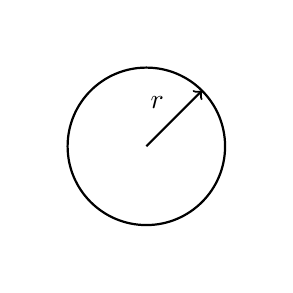
\begin{tikzpicture}
		\draw[white] (-1.5, -1.5) grid (1.5, 1.5);
		\draw[black, thick] (0, 0) circle (1);
		\draw[black, thick, ->] (0, 0) -- node[above left] {$r$} ({cos(45)}, {sin(45)});
	\end{tikzpicture}
\end{minipage}\hfill
\begin{minipage}[c]{0.54\textwidth}
\textbf{Circle.} Radius $r$.
\end{minipage}

\vspace{1em}
\noindent
\begin{minipage}[c]{0.42\textwidth}
	\centering
	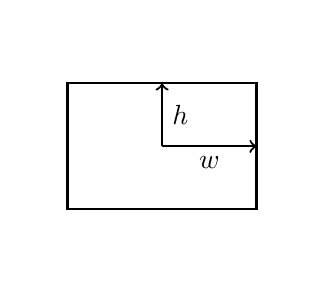
\begin{tikzpicture}
		\draw[white] (-1.7, -1.5) grid (1.7, 1.5);
		\draw[black, thick] (-1.2, -0.8) rectangle (1.2, 0.8);
		\draw[black, thick, ->] (0, 0) -- node[below] {$w$} (1.2, 0);
		\draw[black, thick, ->] (0, 0) -- node[right] {$h$} (0, 0.8);
	\end{tikzpicture}
\end{minipage}\hfill
\begin{minipage}[c]{0.54\textwidth}
\textbf{Rectangle.} Half-width $w$ and half-height $h$.
\end{minipage}

\vspace{1em}
\noindent
\begin{minipage}[c]{0.42\textwidth}
	\centering
	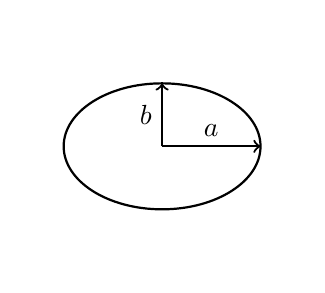
\begin{tikzpicture}
		\draw[white] (-1.7, -1.5) grid (1.7, 1.5);
		\draw[black, thick] (0, 0) ellipse (1.25 and 0.8);
		\draw[black, thick, ->] (0, 0) -- node[above] {$a$} (1.25, 0);
		\draw[black, thick, ->] (0, 0) -- node[left] {$b$} (0, 0.8);
	\end{tikzpicture}
\end{minipage}\hfill
\begin{minipage}[c]{0.54\textwidth}
\textbf{Ellipse.} Half-major axis $a$ and half-minor axis $b$.
\end{minipage}

\vspace{1em}
\noindent
\begin{minipage}[c]{0.42\textwidth}
	\centering
	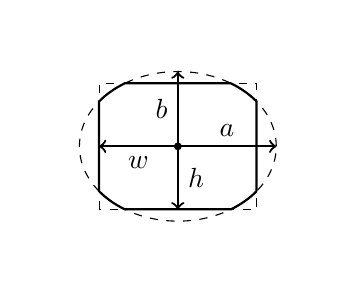
\begin{tikzpicture}
		\pgfmathsetmacro{\rw}{1.0}
		\pgfmathsetmacro{\rh}{0.8}
		\pgfmathsetmacro{\ea}{1.25}
		\pgfmathsetmacro{\eb}{0.95}
		\pgfmathsetmacro{\angA}{acos(\rw/\ea)}
		\pgfmathsetmacro{\angB}{asin(\rh/\eb)}
		\pgfmathsetmacro{\ix}{\ea*cos(\angB)}
		\pgfmathsetmacro{\iy}{\eb*sin(\angA)}
		\draw[white] (-1.9, -1.5) grid (1.9, 1.5);
		\draw[black, dashed] (-\rw, -\rh) rectangle (\rw, \rh);
		\draw[black, thick]
			(\rw, -\iy) -- (\rw, \iy)
			arc[start angle=\angA, end angle=\angB, x radius=\ea, y radius=\eb]
			-- (-\ix, \rh)
			arc[start angle=180-\angB, end angle=180-\angA, x radius=\ea, y radius=\eb]
			-- (-\rw, -\iy)
			arc[start angle=180+\angA, end angle=180+\angB, x radius=\ea, y radius=\eb]
			-- (\ix, -\rh)
			arc[start angle=360-\angB, end angle=360-\angA, x radius=\ea, y radius=\eb];
		\draw[black, dashed] (0, 0) ellipse [x radius=\ea, y radius=\eb];
		\fill[black] (0, 0) circle (0.05);
		\draw[black, thick, ->] (0, 0) -- node[below] {$w$} (-\rw, 0);
		\draw[black, thick, ->] (0, 0) -- node[right] {$h$} (0, -\rh);
		\draw[black, thick, ->] (0, 0) -- node[above] {$a$} (\ea, 0);
		\draw[black, thick, ->] (0, 0) -- node[left] {$b$} (0, \eb);
	\end{tikzpicture}
\end{minipage}\hfill
\begin{minipage}[c]{0.54\textwidth}
\textbf{Rectellipse.} Half-width $w$, half-height $h$, half-major axis $a$, and half-minor axis $b$.
\end{minipage}

\vspace{1em}
\noindent
\begin{minipage}[c]{0.42\textwidth}
	\centering
	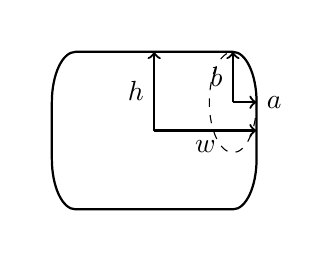
\begin{tikzpicture}
		\draw[white] (-1.6, -1.3) grid (1.6, 1.3);
		\draw[black, thick] \racetrack{0}{0}{1.3}{1}{0.3}{0.64};
		\draw[black, dashed] (1.0, 0.36) ellipse [x radius=0.3, y radius=0.64];
		\draw[black, thick, ->] (0, 0) -- node[below] {$w$} (1.3, 0);
		\draw[black, thick, ->] (0, 0) -- node[left] {$h$} (0, 1.0);
		\draw[black, thick, ->] (1.0, 0.36) -- (1.3, 0.36) node[right] {$a$};
		\draw[black, thick, ->] (1.0, 0.36) -- node[left] {$b$} (1.0, 1.0);
	\end{tikzpicture}
\end{minipage}\hfill
\begin{minipage}[c]{0.54\textwidth}
\textbf{Racetrack.} Half-width $w$, half-height $h$, and ellipse-corner half-axes $a$, $b$.
\end{minipage}

\vspace{1em}
\noindent
\begin{minipage}[c]{0.42\textwidth}
	\centering
	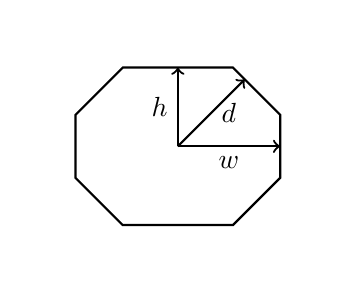
\begin{tikzpicture}
		\pgfmathsetmacro{\ow}{1.3}
		\pgfmathsetmacro{\oh}{1.0}
		\pgfmathsetmacro{\od}{1.7/sqrt(2)}
		\pgfmathsetmacro{\ox}{\od*sqrt(2)-\oh}
		\pgfmathsetmacro{\oy}{\od*sqrt(2)-\ow}
		\pgfmathsetmacro{\of}{\od/sqrt(2)}
		\draw[white] (-1.9, -1.5) grid (1.9, 1.5);
		\draw[black, thick]
			(-\ox, -\oh) -- (\ox, -\oh) -- (\ow, -\oy) -- (\ow, \oy) --
			(\ox, \oh) -- (-\ox, \oh) -- (-\ow, \oy) -- (-\ow, -\oy) -- cycle;
		\draw[black, thick, ->] (0, 0) -- node[below] {$w$} (\ow, 0);
		\draw[black, thick, ->] (0, 0) -- node[left] {$h$} (0, \oh);
		\draw[black, thick, ->] (0, 0) -- node[right] {$d$} (\of, \of);
	\end{tikzpicture}
\end{minipage}\hfill
\begin{minipage}[c]{0.54\textwidth}
\textbf{Octagon.} Half-width $w$, half-height $h$, and half-diagonal gap $d$.
\end{minipage}

\vspace{1em}
\noindent
\begin{minipage}[c]{0.42\textwidth}
	\centering
	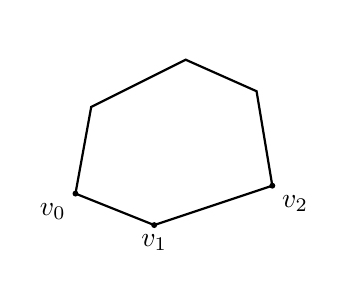
\begin{tikzpicture}
		\draw[white] (-1.9, -1.5) grid (1.9, 1.5);
		\draw[black, thick]
			(-1.3, -0.6) -- (-0.3, -1.0) -- (1.2, -0.5) -- (1.0, 0.7) --
			(0.1, 1.1) -- (-1.1, 0.5) -- cycle;
		\filldraw[black] (-1.3, -0.6) circle (0.03) node[below left] {$v_0$};
		\filldraw[black] (-0.3, -1.0) circle (0.03) node[below] {$v_1$};
		\filldraw[black] (1.2, -0.5) circle (0.03) node[below right] {$v_2$};
	\end{tikzpicture}
\end{minipage}\hfill
\begin{minipage}[c]{0.54\textwidth}
\textbf{Polygon.} Arbitrary polygon given by an ordered list of vertices $(v_0, v_1, \ldots) = ((x_0, y_0), (x_1, y_1), \ldots)$.
\end{minipage}

\subsection{Profiles}

A \emph{profile} comprises of any of the above-mentioned logical shapes.
Tolerances can be specified on a profile installed in a pipe (a \emph{profile position})
and on an installed pipe (a \emph{pipe position}).
At each position, three tolerances can be specified:
\begin{itemize}
    \item \lstinline|tol_r|: radial tolerance,
    \item \lstinline|tol_x|: horizontal tolerance,
    \item \lstinline|tol_y|: vertical tolerance.
\end{itemize}
For each installed aperture, the tolerances of its profile position and pipe position are
added component by component to give the total \lstinline|tol_r|, \lstinline|tol_x|,
and \lstinline|tol_y|.
These totals effectively form a tolerance racetrack with half-width of
$\text{\lstinline|tol_x|} + \text{\lstinline|tol_r|}$, half-height
$\text{\lstinline|tol_y|} + \text{\lstinline|tol_r|}$, and a circular radius of
$\text{\lstinline|tol_r|}$.

%	\begin{tikzpicture}
%		\draw[white] (-2, 2) grid (2, 2);
%		\draw[black, thick]
%			(1.5, -0.5)
%			arc[start angle=0, end angle=-90, radius=0.5]
%			-- (-1.0, -1.0)
%			arc[start angle=-90, end angle=-180, radius=0.5]
%			-- (-1.5, 0.5)
%			arc[start angle=180, end angle=90, radius=0.5]
%			-- (1.0, 1.0)
%			arc[start angle=90, end angle=0, radius=0.5]
%			-- cycle;
%
%		\draw[black, dashed] (1, 0.5) -- (1, -0.5) -- (-1, -0.5) -- (-1, 0.5) -- cycle;
%
%		\draw[black, thick, ->] (0, 0) -- node[below] {$w$} (1.0, 0);
%		\draw[black, thick, ->] (0, 0) -- node[left] {$h$} (0, 0.5);
%		\draw[black, thick, ->] (1.0, 0.5) -- (1.5, 0.5) node[right] {$a$};
%		\draw[black, thick, ->] (1.0, 0.5) -- node[left] {$b$} (1.0, 1.0);
%	\end{tikzpicture}

\subsection{Beam envelope}\label{subsec:apertures-beam-envelope}

The beam-envelope calculation uses:
\begin{itemize}
    \item local optics and closed orbit values,
    \item beam and tolerance parameters specified by the user,
    \item summed aperture tolerances of the local profile position and pipe position.
\end{itemize}
In particular, \lstinline{halo_params} define the following beam parameters:
\begin{itemize}
    \item \lstinline{nemitt_x} ($\varepsilon_{x,\mathrm{n}}$) and
    \lstinline{nemitt_y} ($\varepsilon_{y,\mathrm{n}}$) -- normalised emittances (in metres),
    \item \lstinline{delta_rms} ($\delta_\mathrm{rms}$) -- root-mean-square relative momentum spread (unitless),
    \item \lstinline{tol_co} ($r_\mathrm{co}$) -- closed orbit error (in metres),
    \item \lstinline{tol_disp} ($f_D$) -- dispersion tolerance scaling factor (unitless),
    \item \lstinline{tol_disp_ref} ($D_\mathrm{ref}$) -- reference dispersion error (in metres),
    \item \lstinline{tol_disp_ref_beta} ($\beta_{D,\mathrm{ref}}$) -- reference beta for dispersion scaling (in metres),
    \item \lstinline{tol_beta_beating} ($f_\beta$) -- beta beating tolerance scaling factor (unitless),
    \item $h_x := \frac{\text{\lstinline{halo_x}}}{\text{\lstinline{halo_primary}}}$, $h_y := \frac{\text{\lstinline{halo_y}}}{\text{\lstinline{halo_primary}}}$, and $h_r := \frac{\text{\lstinline{halo_r}}}{\text{\lstinline{halo_primary}}}$ -- reference horizontal, vertical, and radial size of the beam in units of betatron sigma.
\end{itemize}
The optical beam sizes for a one-betatron sigma beam are given by
\[
\sigma_x = \sqrt{\frac{\varepsilon_{x,\mathrm{n}}}{\gamma_r\beta_r}\beta_x} \cdot f_\beta,
\qquad
\sigma_y = \sqrt{\frac{\varepsilon_{y,\mathrm{n}}}{\gamma_r\beta_r}\beta_y} \cdot f_\beta.
\]
We model the beam as a racetrack of shape determined by the parameters $h_x$, $h_y$, and $h_r$.
To obtain the modelled $n$-sigma beam envelope in metres, the racetrack defined by the above parameters is scaled by $(n\sigma_x, n\sigma_y)$:
\[
	n \cdot \text{\lstinline{beam_racetrack}} :=
	n
	\begin{bmatrix}
	  \sigma_x \\
	  \sigma_y 
	\end{bmatrix}
	\cdot
	\begin{tikzpicture}[baseline={(0, -1mm)}]
		\draw[white] (-1.6, -1.2) grid (1.6, 1.2);
		\draw[black, thick] \racetrack{0}{0}{1.5}{1}{0.5}{0.5};

		%\draw[black, dashed] (1, 0.5) circle (0.5);
		\draw[black, dashed] (1, 0.5) -- (1, -0.5) -- (-1, -0.5) -- (-1, 0.5) -- cycle;

		\draw[black, thick, ->] (0, 0) -- node[below] {$h_x$} (1.5, 0);
		\draw[black, thick, ->] (0, 0) -- node[left] {$h_y$} (0, 1);

		\draw[black, thick, ->] (0, 0) -- node[above] {$h_r$} ($(1.0, 0.5) + (26.6:0.5)$);
	\end{tikzpicture}
\]
Separately, we can build a tolerance racetrack which includes:
\begin{itemize}
    \item the summed aperture tolerances \lstinline|tol_x|, \lstinline|tol_y|,
    \lstinline|tol_r|,
    \item uncorrelated (also referred to as \emph{spurious}) dispersion orbit shift:
    \[
		\Delta x_{D,\beta} := f_\beta \cdot f_D \cdot D_\mathrm{ref} \cdot \sqrt{\frac{\beta_x}{\beta_{D,\mathrm{ref}}}} \cdot \delta_\mathrm{rms},
		\qquad
		\Delta y_{D,\beta} := f_\beta \cdot f_D \cdot D_\mathrm{ref} \cdot \sqrt{\frac{\beta_y}{\beta_{D,\mathrm{ref}}}} \cdot \delta_\mathrm{rms},
	\]
    \item and the closed-orbit tolerance $r_\mathrm{co}$.
\end{itemize}
This racetrack can be visualised as (where $+$ denotes convolution/Minkowski sum):
\[
	\text{\lstinline{halo_racetrack}} :=
	\begin{tikzpicture}[baseline={(0, -1mm)}]
		\draw[black, thick] \racetrack{0}{0}{1.2}{1}{0.5}{0.5};

		%\draw[black, dashed] (1, 0.5) circle (0.5);
		\draw[black, dashed] (0.7, 0.5) -- (0.7, -0.5) -- (-0.7, -0.5) -- (-0.7, 0.5) -- cycle;

		\draw[black, thick, ->] (0, 0) -- node[below] {\ttlabel{tol_x}} (0.7, 0);
		\draw[black, thick, ->] (0, 0) -- node[left] {\ttlabel{tol_y}} (0, 0.5);

		\draw[black, thick, ->] (0.7, 0.5) -- node[left] {\ttlabel{tol_r}} ($(0.7, 0.5) + (45:0.5)$);
	\end{tikzpicture}
	\;+\;
	\begin{tikzpicture}[baseline={(0, -1mm)}]
		\draw[black, thick] (0, 0) ellipse (1.25 and 0.8);
		\draw[black, thick, ->] (0, 0) -- node[below left = 0 and -4mm] {$\Delta x_{D,\beta}$} (1.25, 0);
		\draw[black, thick, ->] (0, 0) -- node[below left = -2mm and -1mm] {$\Delta y_{D,\beta}$} (0, 0.8);
	\end{tikzpicture}
	\;+\;
		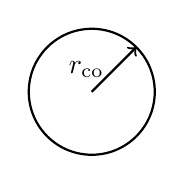
\begin{tikzpicture}[baseline={(0, -1mm)}]
		\draw[black, thick] (0, 0) circle (0.8);
		\draw[black, thick, ->] (0, 0) -- node[left] {$r_\mathrm{co}$} (45:0.8);
	\end{tikzpicture}
\]
Since racetracks are closed under convolution, we can represent our beam envelope at $n$-sigmas (without including correlated dispersion orbit shift yet) as:
\[
	\text{\lstinline{envelope}}(n) := \text{\lstinline{halo_racetrack}} + n \cdot \text{\lstinline{beam_racetrack}}.
\]
Depending on the algorithm this representation will be converted to a polygon (beam envelope generation functions, bisection method for computing the max aperture sigma) or will be used directly for analytic calculations.

In aperture calculations we must further include the orbit shift error induced by correlated dispersion, also referred to as \emph{model} dispersion.
In the case of converting to a polygon, we can further include this orbit shift in the resulting shape by `stretching' it.
We can convolve $\text{\lstinline{envelope}}(n)$ with the line segment $[-\mathbf{v}_{D,\mathrm{model}}, \mathbf{v}_{D,\mathrm{model}}]$, where
\[
	\mathbf{v}_{D,\mathrm{model}} := \begin{bmatrix}
	  D_x \delta_\mathrm{rms} \\
	  D_y \delta_\mathrm{rms}
	\end{bmatrix},
\]
to obtain an $n$-sigma beam envelope including the error related to correlated dispersion, as well as uncorrelated dispersion error, aperture tolerance, and closed-orbit tolerance errors.
In the case of analytic methods, we will usually separately consider two envelopes shifted by $\pm\mathbf{v}_{D,\mathrm{model}}$ instead.

\section{Algorithms}

\subsection{Aperture bounds}

For any installed profile let (where by pose we mean the position and orientation)
\begin{itemize}
	\item $M_S$ be the pose of the pipe's survey reference point in the survey frame,
	\item $M_T$ be the pose of the pipe's origin $(x, y, s) = (0, 0, 0)$ relative to the survey reference point,
	\item $M_P$ be the pose representing the installed profile's position within the pipe frame.
\end{itemize}
Then, $M_{P,\mathrm{world}} = M_S \, M_T \, M_P$ represents the position and orientation of the installed profile in world coordinates (survey frame).
In order to calculate the locations of the installed profiles in the survey frame, we perform the intersection of the profile plane (local $s = 0$ in the $M_{P,\mathrm{world}}$ frame) with the survey curve.
Each segment of the survey is defined as either a line segment or an arc segment, and we work our way outwards from the survey reference point testing for intersection, until a valid $s$ is found.
The bounds $s_\mathrm{start}$ and $s_\mathrm{end}$ are computed by projecting each 3D polygon point of a given installed profile onto the survey curve and taking the minimum and maximum values.

As mentioned in this chapter's introduction, aperture bounds are used for checking the validity of the model as well as for aperture interpolation.
Validation checks that each installed pipe's survey reference is consistent and that
the longitudinal intervals covered by different pipes' profile-centre positions do not
overlap by more than \lstinline{s_tol}.
These intervals are distinct from the projected profile footprints, which can overlap.
For rings, the validation accounts for pipes crossing the end of the survey.

\subsection{Cross section interpolation}

The module is capable of computing the aperture polygons in the plane orthogonal to an arbitrary $s$-position along the survey.
Aperture bounds are used to find the correct installed apertures that need to be interpolated.
If the $s$ position for interpolation sits outside of any bounds, we interpolate the profiles on either side of $s$.
However, if the $s$ position sits within a bound of some aperture $i$, we need to partly interpolate $i - 1$ with $i$, and partly interpolate $i$ with $i + 1$.
This is illustrated in Figures~\ref{fig:aperture-interpolation-simple} and~\ref{fig:aperture-interpolation-both-sides}.
Profile-position tolerances are interpolated linearly in $s$ between neighbouring
profile centres within the same installed pipe, and the active pipe-position tolerances
are added to the result.
Across a pipe boundary, tolerances retain the active installed profile's summed values;
they are not interpolated between pipes, although the aperture geometry is.

\begin{figure}
	\centering
	\begin{tikzpicture}
		\draw[black, thick, ->] (-3, 0) -- (3.5, 0) node[below right] {$\hat{s}$};

		\draw[black, thick] (-1.3, -1.2) -- (-0.7, 1.2);
		\draw[black, dashed] (-1.3, -1.2) -- (-1.3, 0);
		\draw[black, dashed] (-0.7, 1.2) -- (-0.7, 0);

		\draw[black, thick] (1.9, -1.5) -- (1.3, 1.5);		
		\draw[black, dashed] (1.9, -1.5) -- (1.9, 0);
		\draw[black, dashed] (1.3, 1.5) -- (1.3, 0);
		
		\draw[red, thick] (0.3, 1.35) -- (0.3, -1.35);
		
		\fill[black] (0.3, 0) circle (0.05) node[below right] {$s_q$};
		\draw[black, dashed] (0.3, -2) -- (0.3, 2);
		\draw[black]  (0.3, 0.2) -- (0.5, 0.2) -- (0.5, 0);

		\draw[black, dotted] (-0.7, 1.2) -- (1.3, 1.5);
		\fill[black] (0.3, 1.35) circle (0.05) node[above left] {$P$};

		\draw[black, dotted] (-1.3, -1.2) -- (1.9, -1.5);
		\fill[black] (0.3, -1.35) circle (0.05) node [below left] {$Q$};
	\end{tikzpicture}
	\caption{Visualisation of aperture interpolation at some $s_q$ outside of any aperture bounds. The points $P$ and $Q$ are obtained by interpolating corresponding vertices of profiles on either side of $s_q$.}\label{fig:aperture-interpolation-simple}
\end{figure}

\begin{figure}
	\centering
	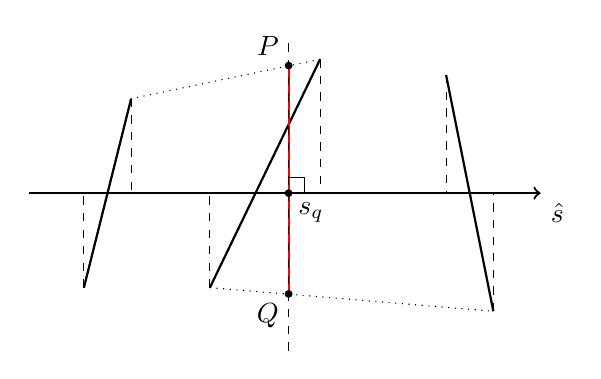
\begin{tikzpicture}
		\draw[black, thick, ->] (-3, 0) -- (3.5, 0) node[below right] {$\hat{s}$};

		\draw[black, thick] (-0.7, -1.2) -- (0.7, 1.7);
		\draw[black, dashed] (-0.7, -1.2) -- (-0.7, 0);
		\draw[black, dashed] (0.7, 1.7) -- (0.7, 0);
		%\fill[black] (-0.12, 0) circle (0.05);
		
		\draw[black, thick] (-2.3, -1.2) -- (-1.7, 1.2);
		\draw[black, dashed] (-2.3, -1.2) -- (-2.3, 0);
		\draw[black, dashed] (-1.7, 1.2) -- (-1.7, 0);
		
		\draw[black, thick] (2.9, -1.5) -- (2.3, 1.5);
		\draw[black, dashed] (2.9, -1.5) -- (2.9, 0);
		\draw[black, dashed] (2.3, 1.5) -- (2.3, 0);
		
		\draw[red, thick] (0.3, 1.62) -- (0.3, -1.28);
		
		\fill[black] (0.3, 0) circle (0.05) node[below right] {$s_q$};
		\draw[black, dashed] (0.3, -2) -- (0.3, 2);
		\draw[black]  (0.3, 0.2) -- (0.5, 0.2) -- (0.5, 0);
		
		\draw[black, dotted] (0.7, 1.7) -- (-1.7, 1.2);
		\fill[black] (0.3, 1.62) circle (0.05) node[above left] {$P$};
		
		\draw[black, dotted] (-0.7, -1.2) -- (2.9, -1.5);
		\fill[black] (0.3, -1.28) circle (0.05) node[below left] {$Q$};
	\end{tikzpicture}
	\caption{If $s_q$ falls within bounds of an installed aperture, some of the vertices of the new cross section need to be interpolated with the aperture to the left, such as point $P$, while other ones with the aperture to the right, such as point $Q$.}\label{fig:aperture-interpolation-both-sides}
\end{figure}

For a query at longitudinal position $s$, interpolation is performed in the cross-section
plane defined by the resampled survey pose at that $s$.
The active profile is selected from the bound containing $s$, or the immediately preceding
bound when $s$ lies between bounds.
The target plane and neighbouring installed profiles are brought into the active profile's
pipe frame.
This is done to limit numerical noise that might otherwise be present when mixing small local quantities with world coordinates.

The profiles are uniformly discretised into the same number of points and the first step before actual interpolation is determining point correspondence between the profiles.
This is done after projecting the neighbouring polygons into the target cross-section plane.
The vertex order is reversed if the projected orientations differ, and a cyclic shift is
chosen to minimise the sum of squared distances between corresponding vertices.
Interpolation then proceeds by connecting corresponding 3D vertices from the two neighbouring installed profiles and intersecting those line segments with the target plane.

Between profiles of different installed pipes, interpolation uses straight segments.
Within a curved pipe, the following approximation is employed.
Note that, for a curved pipe, $M_P$ already includes the motion along the curved reference axis, i.e. the profile is first advanced by the pipe curvature to its local $s$-location and then given its local offsets/rotations.
During interpolation, the segment-plane intersection is handled after `straightening' the curvilinear frame.
Given a Cartesian frame and a curvilinear frame with curvature $h$ (or equivalently radius $R = h^{-1}$) whose origins coincide, a Cartesian point can be transformed into a curvilinear point as follows:
\[
	\begin{bmatrix} x \\ y \\ s \end{bmatrix} =
	\begin{bmatrix}
		\mathrm{sgn}(h) \sqrt{(X+R)^2+Z^2}-R \\
		Y \\
		R \cdot \mathrm{atan}_2\left(\mathrm{sgn}(h) Z,\, \mathrm{sgn}(h)(X + R)\right)
	\end{bmatrix}.
\]
We can transform a plane, which is represented as a (Cartesian) normal $(v_X, v_Y, v_Z)$ attached to a (curvilinear) point $(x, y, s)$, like so:
\[
	\begin{bmatrix} v_x \\ v_y \\ v_s \end{bmatrix} =
	\begin{bmatrix}
		\cos(hs) & 0 & \sin(hs) \\
		0 & 1 & 0 \\
		-\frac{\sin(hs)}{1+h x} & 0 & \frac{\cos(hs)}{1+h x}
	\end{bmatrix}
	\begin{bmatrix} v_X \\ v_Y \\ v_Z \end{bmatrix}.
\]
Once the two polygon points together with the plane's point and normal are transformed, we can perform the intersection in the `straightened' frame with the usual algorithm.
The resulting point can be converted back to the Cartesian plane with:
\[
	\begin{bmatrix} X \\ Y \\ Z \end{bmatrix} =
	\begin{bmatrix}
        (R + x) \cos(h s) - R \\
        y \\
        (R + x) \sin(h s)
    \end{bmatrix}.
\]

\subsection{Maximum beam sigma}

There are three methods currently implemented for computing the maximum number of sigmas for which the beam fits in a given cross section; this quantity is often referred to as $n_1$:
\begin{equation}\label{eq:apertures-n1}
	n_1 := \sup \left\{ n \;|\; \text{\lstinline{total_envelope}}(n) \subset \text{\lstinline{cross_section}} \right\}.
\end{equation}
The \lstinline{total_envelope} corresponds to \lstinline{envelope} with the correlated dispersion error applied; the precise method of the application of this error, and the computation of $n_1$ is what distinguishes the three different algorithms implemented in Xtrack.
These algorithms are described below.

\subsubsection{`Bisection' method}

The \emph{bisection} method computes $n_1$ as the largest beam scale factor for which the full beam envelope polygon still fits inside the interpolated aperture polygon.
In particular, the beam envelope is discretised to a polygon which includes the dispersive orbit error as a `stretch' described in Section~\ref{subsec:apertures-beam-envelope}, and visualised in Fig.~\ref{fig:aperture-bisection}.
At each $s$ a trial envelope is repeatedly built, the algorithm checks polygon containment, and bisects until the limiting value is found.
It is the most direct geometric implementation of Eq.~\ref{eq:apertures-n1}, but also the most expensive at  $O(EAK)$, where $E$ is the number of envelope points,
              $A$ is the number of aperture points, and $K = \log_2(\frac{\text{search space}}{\text{search tolerance}})$ is the number of bisection steps, currently $K \leq 25$.

\begin{figure}
	\centering
	\begin{tikzpicture}
		\draw[white] (-4, -3) grid (4, 3);
		
		\draw[black, dashed] \racetrack{0}{0}{1.5}{1}{0.5}{0.5};
		\draw[black, dashed] \racetrack{1.35}{0.85}{0.8}{1.2}{0.8}{1.2};
		\draw[black, dashed] \racetrack{0}{0}{2.3}{2.2}{1.3}{1.7};
		
		\draw[black] (-0.07, -0.07) -- (0.07, 0.07); \draw[black] (0.07, -0.07) -- (-0.07, 0.07);
		\draw[black, ->] ($(-1, 0.5) + (-220:1.3 and 1.7)$) -- ++(-0.5, 0.5) node[left] {\footnotesize$\mathbf{v}_{D,\text{model}}$};
		\draw[black, ->] ($(1, -0.5) - (-220:1.3 and 1.7)$) -- ++(0.5, -0.5) node[right] {\footnotesize$-\mathbf{v}_{D,\text{model}}$};
		
		\draw[black, thick] ({0 + 2.3 + 0.5}, {0 - 2.2 + 1.7 - 0.5})
		    arc[start angle=0, end angle=-90, x radius=1.3, y radius=1.7]
		    -- ({0 - 2.3 + 1.3 + 0.5}, {0 - 2.2 - 0.5})
		    arc[start angle=-90, end angle=-130, x radius=1.3, y radius=1.7]
		    -- ++(-1, 1)
		    arc[start angle=-130, end angle=-180, x radius=1.3, y radius=1.7]
		    -- ({0 - 2.3 - 0.5}, {0 + 2.2 - 1.7 + 0.5})
		    arc[start angle=180, end angle=90, x radius=1.3, y radius=1.7]
		    -- ({0 + 2.3 - 1.3 - 0.5}, {0 + 2.2 + 0.5})
		    arc[start angle=90, end angle=50, x radius=1.3, y radius=1.7]
		    -- ++(1, -1)
		    arc[start angle=50, end angle=0, x radius=1.3, y radius=1.7]
		    -- cycle;
		
		\draw (0, -1) node[below] {\footnotesize\lstinline{halo_rt}};
		\fill[black] (1.35, 0.85) circle (0.05);
		\draw (1.35, {0.85 - 1.2}) node[below] {\footnotesize$n \, \text{\lstinline{beam_rt}}$};
		\draw (0, -2.7) node[below] {\footnotesize$\text{\lstinline{total_envelope}}(n) := \text{\lstinline{halo_rt}} + n \cdot \text{\lstinline{beam_rt}} + [-\mathbf{v}_{D,\text{model}}, \mathbf{v}_{D,\text{model}}]$};
	\end{tikzpicture}
	\caption{The construction of the \lstinline{total_envelope} used in the \emph{bisection} method. The $\times$ symbol marks the closed orbit. The envelope is repeatedly converted to a polygon for different $n$, until a limiting value for containment within the aperture is found through bisection.}\label{fig:aperture-bisection}
\end{figure}

\subsubsection{`Rays' method}

The \emph{rays} method approximates the same limit by sampling a finite set of angles $\theta$.
For each ray direction $\theta$, it computes the distances $d_\mathrm{halo}$, $d_\mathrm{envelope}$, and $d_\mathrm{aper}$ from the closed orbit to the \verb|halo_racetrack|, $\text{\lstinline{envelope}}(1)$, and \verb|aperture|, respectively, as visualised in Fig.~\ref{fig:aperture-rays}.
This calculation is analytical using a ray-at-$\theta$--racetrack intersection formula.
These are used to obtain a linear approximation of $n_1 \approx \frac{d_\mathrm{aper} - d_\mathrm{halo}}{d_\mathrm{envelope} - d_\mathrm{halo}}$, which is then used to refine the result using Newton's method.
The dispersion-related orbit shift is included in the method by picking the more pessimistic of the two centroid options when calculating the distances.
The \emph{rays} method is much faster than bisection at $O(\text{number of rays})$, but its accuracy depends on the angular sampling density and can be inaccurate for very flat beams, due to the fact that the sampling is done along a single uniform direction $\theta$.

\begin{figure}
	\centering
	\begin{tikzpicture}
		\draw[white] (-4, -3) grid (4, 3);
		
		\draw[black] \racetrack{0}{0}{1.5}{1}{0.5}{0.5};
		\draw[black] \racetrack{0}{0}{2.3}{2.2}{1.3}{1.7};
		
		\draw[black] ($(0.9, -0.5) + (-0.07, -0.07)$) -- ($(0.9, -0.5) + (0.07, 0.07)$); \draw[black] ($(0.9, -0.5) + (0.07, -0.07)$) -- ($(0.9, -0.5) + (-0.07, 0.07)$);
		\draw[black, ->] (0.9, -0.5) -- (0, 0) node[left] {\footnotesize$\pm\mathbf{v}_{D,\text{model}}$};
		
		\draw (0, -1) node[below] {\footnotesize\lstinline{halo_rt}};
		\draw (0, -2.2) node[below] {\footnotesize$\text{\lstinline{halo_rt}} + 1 \cdot \text{\lstinline{beam_rt}}$};
		
		\draw (5, -3) node[above right] {\footnotesize\lstinline{cross_section}} -- (5, 3) -- (3, 5) -- (-3, 5);
		
		\draw[black, dashed] (0, 0) -- (0.8, 0);
		\draw[black] (0.5, 0) node[above right] {\footnotesize$\theta$} arc (0:70:0.3);
		\draw[black, dashed] (0, 0) -- ($(7 * 0.766, 7 * 0.643)$);
		
		\fill ($(1.52 * 0.766, 1.52 * 0.643)$) circle (0.05) node[above left] {\footnotesize$d_\text{halo}$};
		\fill ($(2.56 * 0.766, 2.56 * 0.643)$) circle (0.05) node[right=2mm] {\footnotesize$d_\text{envelope}$};
		\fill ($(5.68 * 0.766, 5.68 * 0.643)$) circle (0.05) node[left=2mm] {\footnotesize$d_\text{aper}$};
	\end{tikzpicture}
	\caption{Let $t(\theta, n)$ be the length of the ray at angle $\theta$ intersecting $\text{\lstinline{envelope}}(n)$. The \emph{rays} method finds the value of $n_1$ such that $t(\theta, n_1) - d_\text{aper} = 0$ for each $\theta$. Solving this is a nonlinear problem (and in fact quartic), so we employ Newton's method with an initial linearly approximated guess $n_1 \approx \frac{d_\mathrm{aper} - d_\mathrm{halo}}{d_\mathrm{envelope} - d_\mathrm{halo}}$. For each $\theta$, two centroids are considered for each of the $-\mathbf{v}_{D,\text{model}}$ and $\mathbf{v}_{D,\text{model}}$ (the $\times$ symbol marks the closed orbit), and the smaller of the two values is taken, to include the dispersion-related orbit shift error.}\label{fig:aperture-rays}
\end{figure}

\subsubsection{`Exact' method}

The \emph{exact} method is similar to \emph{rays} in that it evaluates $n_1$ using analytically obtained distances.
Instead of scanning a single set of rays, the search is performed along two sets of rays, as visualised in Fig.~\ref{fig:aperture-exact}.
First, the beam centroids are computed along one set of rays, using the \verb|halo_racetrack| and including the dispersion-related orbit shift.
Then, for each centroid position, another set of rays is emitted to calculate
$d_\text{aper}$, the distance to the aperture from that point, and $d_\text{envelope}$,
the distance to the boundary of the one-sigma \lstinline{beam_racetrack} centred there.
The halo tolerances are already included in the centroid position.
Once the most pessimistic case is found, $n_1 := \frac{d_\text{aper}}{d_\text{envelope}}$.
This method is slower than \emph{rays}, as the complexity is $O((\text{number of rays})^2)$; it is nevertheless more performant than bisection.

\begin{figure}
	\centering
	\begin{tikzpicture}
		\draw[white] (-4, -3) grid (4, 3);
		
		\draw[black, dashed] \racetrack{0}{0}{1.5}{1}{0.5}{0.5};
		\draw[black] \racetrack{1.35}{0.85}{0.8}{1.2}{0.8}{1.2};
		
		\draw[black] ($(0.9, -0.5) + (-0.07, -0.07)$) -- ($(0.9, -0.5) + (0.07, 0.07)$); \draw[black] ($(0.9, -0.5) + (0.07, -0.07)$) -- ($(0.9, -0.5) + (-0.07, 0.07)$);
		\draw[black, ->] (0.9, -0.5) -- (0, 0) node[below left=1mm and -5mm] {\footnotesize$\pm\mathbf{v}_{D,\text{model}}$};
		
		\draw (0, -1) node[below] {\footnotesize\lstinline{halo_rt}};
		\draw (5, -2) node[above right] {\footnotesize\lstinline{cross_section}} -- (5, 3) -- (3, 5) -- (-2, 5);
		
		\fill[black] (1.35, 0.85) circle (0.05);
		\draw (1.35, {0.85 + 1.2}) node[above] {\footnotesize$1 \cdot \text{\lstinline{beam_rt}}$};

		\draw[black, dashed] (0, 0) -- ++(0.8, 0);
		\draw[black] (0.5, 0) arc (0:48:0.3) node[above left=-1mm and -1mm] {\footnotesize$\theta_1$};
		\draw[black, dashed] (0, 0) -- (1.35, 0.85);

		\draw[black, dashed] (1.35, 0.85) -- ++(0.8, 0);
		\draw[black] (1.85, 0.85) arc (0:70:0.3) node[above left=-1mm and -1mm] {\footnotesize$\theta_2$};
		\draw[black, dashed] (1.35, 0.85) -- ($(1.35, 0.85) + (6 * 0.766, 6 * 0.643)$);
	
		\fill ($(1.35, 0.85) + (0.91 * 0.766, 0.91 * 0.643)$) circle (0.05) node[right=2mm] {\footnotesize$d_\text{envelope}$};
		\fill ($(1.35, 0.85) + (4.12 * 0.766, 4.12 * 0.643)$) circle (0.05) node[left=2mm] {\footnotesize$d_\text{aper}$};
	\end{tikzpicture}
	\caption{The \emph{exact} method finds $n_1$ as the minimum value of $\frac{d_\text{aper}}{d_\text{envelope}}$ across all $\theta_1$, $\theta_2$, and considering both $-\mathbf{v}_{D,\text{model}}$ and $\mathbf{v}_{D,\text{model}}$ closed orbit shifts (the $\times$ symbol marks the closed orbit).}\label{fig:aperture-exact}
\end{figure}

